\documentclass[12pt,twoside]{mitthesis}

%%%%%%%%%%%%%%%%%%%%%%%%%%%%%%%%%%%%%%%%%%%%%%%%%%%%%%%%%%%%%%%%%%%%%%%%%%%%%%%%
% PREAMBLE

\usepackage[bitstream-charter]{mathdesign} % Use BT Charter font
\usepackage[T1]{fontenc}                   % Use T1 encoding instead of OT1
\usepackage[utf8]{inputenc}                % Use UTF8 input encoding
\usepackage{microtype}                     % Improve typography
\usepackage{amsmath}                       % AMS Math extensions
\usepackage{booktabs}                      % Improve table spacing
\usepackage{graphicx}                      % Extended graphics capabilities
\usepackage{tocbibind}                     % Include listings in TOC

\usepackage{listings}                      % Source code listings
\usepackage{caption}
\usepackage{subcaption}
\usepackage{color}
\usepackage{url}
\usepackage{array}

\usepackage[breaklinks=true]{hyperref}
\hypersetup{colorlinks=true, linkcolor=black, citecolor=black, urlcolor=black,
  pdftitle={Parallel Algorithms for Monte Carlo Particle Transport Simulation on
    Exascale Computing Architectures},
  pdfauthor={Paul K. Romano}
}
\pagestyle{plain}

\usepackage{floatrow}
\floatsetup[table]{style=plaintop}
\floatsetup[widefigure]{margins=hangleft}

% Algorithm constructs
\usepackage[chapter]{algorithm} % Provides algorithm environment
\usepackage{algorithmicx}       % Provides algorithmic block
\usepackage{algpseudocode}      % Option of algorithmicx package
\renewcommand{\thealgorithm}{\thechapter-\arabic{algorithm}}

% Configure captions
\captionsetup{labelfont=bf, labelsep=colon}
\captionsetup[algorithm]{labelfont=bf, labelsep=colon}

% Use Latin Modern for typewriter fonts
\renewcommand{\ttdefault}{lmtt}

% Add \unit macro
\newcommand{\unit}[1]{\ensuremath{\, \mathrm{#1}}}

\definecolor{gray}{rgb}{0.4,0.4,0.4}
\definecolor{darkblue}{rgb}{0.0,0.0,0.6}
\definecolor{cyan}{rgb}{0.0,0.6,0.6}
\lstset{
  basicstyle=\footnotesize\ttfamily,
  columns=fullflexible,
  showstringspaces=false,
  commentstyle=\color{gray}\upshape,
  frame=single,
  xleftmargin=0.55in
}

\lstdefinelanguage{XML}
{
  morestring=[b]",
  morestring=[s]{>}{<},
  morecomment=[s]{<?}{?>},
  morecomment=[s]{<!--}{-->},
  stringstyle=\color{black},
  identifierstyle=\color{darkblue},
  keywordstyle=\color{cyan},
  morekeywords={}
}

\setcounter{secnumdepth}{4}
\setcounter{tocdepth}{3}

\graphicspath{{figures/ch4/}}
\renewcommand{\contentsname}{Table of Contents}
\renewcommand{\bibname}{References}

\begin{document}

%%%%%%%%%%%%%%%%%%%%%%%%%%%%%%%%%%%%%%%%%%%%%%%%%%%%%%%%%%%%%%%%%%%%%%%%%%%%%%%%
% TITLE PAGE

\title{Parallel Algorithms for Monte Carlo Particle Transport Simulation on
  Exascale Computing Architectures}

\author{Paul Kollath Romano}
\prevdegrees{B.S., Rensselaer Polytechnic Institute (2007) \\
             M.S., Massachusetts Institute of Technology (2009)}
\department{Department of Nuclear Science and Engineering}
\degree{Doctor of Philosophy in Nuclear Science and Engineering}

\degreemonth{February}
\degreeyear{2013}
\thesisdate{January 11, 2013}

\supervisor{Benoit Forget}{Assistant Professor of Nuclear Science and
  Engineering}
\reader{Kord S. Smith}{Professor of the Practice of Nuclear Science and
  Engineering}
\chairman{Mujid S. Kazimi}{Chairman, Department Committee on Graduate Students}

\maketitle

%%%%%%%%%%%%%%%%%%%%%%%%%%%%%%%%%%%%%%%%%%%%%%%%%%%%%%%%%%%%%%%%%%%%%%%%%%%%%%%
% ABSTRACT

\cleardoublepage
\setcounter{savepage}{\thepage}

\begin{abstractpage}
Monte Carlo particle transport methods are being considered as a viable option
for high-fidelity simulation of nuclear reactors. While Monte Carlo methods
offer several potential advantages over deterministic methods, there are a
number of algorithmic shortcomings that would prevent their immediate adoption
for full-core analyses. In this thesis, algorithms are proposed both to
ameliorate the degradation in parallal efficiency typically observed for large
numbers of processors and to offer a means of decomposing large tally data that
will be needed for reactor analysis.

A nearest-neighbor fission bank algorithm was proposed and subsequently
implemented in the OpenMC Monte Carlo code. A theoretical analysis of the
communication pattern shows that the expected cost is $O(\sqrt{N})$ whereas
traditional fission bank algorithms are $O(N)$ at best. The algorithm was tested
on two supercomputers, the Intrepid Blue Gene/P and the Titan Cray XK7, and
demonstrated nearly linear parallel scaling up to 163,840 processor cores on a
full-core benchmark problem.

An algorithm for reducing network communication arising from tally reduction was
analyzed and implemented in OpenMC. The proposed algorithm groups only particle
histories on a single processor into batches for tally purposes --- in doing so
it prevents all network communication for tallies until the very end of the
simulation. The algorithm was tested, again on a full-core benchmark, and shown
to reduce network communication substantially.

A model was developed to predict the impact of load imbalances on the
performance of domain decomposed simulations. The analysis demonstrated that
load imbalances in domain decomposed simulations arise from two distinct
phenomena: non-uniform particle densities and non-uniform spatial leakage. The
dominant performance penalty for domain decomposition was shown to come from
these physical effects rather than insufficient network bandwidth or high
latency. The model predictions were verified with measured data from simulations
in OpenMC on a full-core benchmark problem.

Finally, a novel algorithm for decomposing large tally data was proposed,
analyzed, and implemented/tested in OpenMC. The algorithm relies on disjoint
sets of compute processes and tally servers. The analysis showed that for a
range of parameters relevant to LWR analysis, the tally server algorithm should
perform with minimal overhead. Tests were performed on Intrepid and Titan and
demonstrated that the algorithm did indeed perform well over a wide range of
parameters.
\end{abstractpage}


\cleardoublepage

%%%%%%%%%%%%%%%%%%%%%%%%%%%%%%%%%%%%%%%%%%%%%%%%%%%%%%%%%%%%%%%%%%%%%%%%%%%%%%%
% ACKNOWLEDGMENTS

\section*{Acknowledgments}

This research was performed under appointment to the Rickover Fellowship Program
in Nuclear Engineering sponsored by Naval Reactors Division of the
U.S. Department of Energy. This work was also supported in part by the Office of
Advanced Scientific Computing Research, Office of Science, US Department of
Energy, under Contract DE-AC02-06CH11357 and by the Consortium for Advanced
Simulation of Light Water Reactors, an Energy Innovation Hub for Modeling and
Simulation of Nuclear Reactors under US Department of Energy Contract
No. DE-AC05-00OR22725.

I would like to express my most sincere gratitude to my advisor, Ben Forget, for
his unconditional support over the years, for granting me pretty much complete
autonomy in pursuing my research, and yet still providing the vision and
necessary guidance to work towards a tangible goal. I could not have asked for a
better advisor, mentor, or friend to have during my years as a graduate student.

I have been most fortunate to also have Kord Smith serve in an advisory capacity
in my work. Kord has helped us tremendously with keeping a focus on realistic
problems and one day bringing OpenMC to a point where it could be used for real
analysis. I am certainly indebted to him, not only for his advice, lectures, and
inspiration, but also for the many drinks that he has subsidized.

It has truly been an honor working closely with Andrew Siegel on the development
of parallel algorithms. His guidance was instrumental in the successful analysis
and implementation of our tally server methodology. I also thank him for his
mentorship on various issues, and look forward to future collaborations
together.

Also deserving acknowledgment are Tom Sutton, Tim Trumbull, and Forrest Brown
for their patience and willingness to answer my many questions on Monte Carlo
methods. My growth as a competant methods developer would not have been possible
without their counsel. I would also like to thank Tim Donovan for his help in
navigating the public utterance process.

Feedback from the nascent OpenMC user and developer community has significantly
improved the usability and performance of the code --- a big thanks to Andrew
Siegel, Bryan Herman, Katie Biegel, Jed Phillips, Steven Fine, Nick Horelik, and
Adam Nelson for all that they've done in this respect.

The five and a half years that I've spent in graduate school have been
incredible thanks to my friends and family all over the country who have
provided constant encouragement in all my pursuits. Finally, I want to thank my
wife and best friend, Audrey, without whose love, understanding, and support,
this would have not been possible. She has pushed me out of my zone of comfort
and opened my eyes to the world, quite literally.

\pagestyle{plain}

%%%%%%%%%%%%%%%%%%%%%%%%%%%%%%%%%%%%%%%%%%%%%%%%%%%%%%%%%%%%%%%%%%%%%%%%%%%%%%%
% TABLE OF CONTENTS, FIGURES, TABLES

\begin{singlespace}
\tableofcontents
\newpage
\listoffigures
\newpage
\listoftables
\end{singlespace}

%%%%%%%%%%%%%%%%%%%%%%%%%%%%%%%%%%%%%%%%%%%%%%%%%%%%%%%%%%%%%%%%%%%%%%%%%%%%%%%
% CHAPTERS

\chapter{Introduction}
\label{chap:intro}

\section{The Monte Carlo Method}

At the heart of nuclear engineering and many associated fields is the study of
the behavior of subatomic particles interacting with matter. Reactor engineers
are interested in the distribution of power and other reaction rates at each
point in a nuclear reactor; medical physicists are interested in energy
deposition in the human body due to radiation treatments; nuclear
astrophysicists are interested in how nuclear reactions can produce elements
heavier than hydrogen in stars; and so on. In order to determine such
quantities, one generally needs knowledge of two things:
\begin{enumerate}
\item An understanding of how individual particles interact with the matter
  through which they're traveling; and
\item A mathematical description for how a distribution of particles evolves in
  time.
\end{enumerate}
The study of particle interactions is of primary concern to nuclear
physicists. The advent of quantum mechanics in the early 20th century greatly
advanced the state of understanding of particle interactions, especially with
respect to the scattering of particles, a subject which can not be understood
well without considering quantum effects. The latter subject, i.e. the theory of
particle transport, came to maturity in the middle and later parts of the 20th
century, with many advances coming from the nuclear reactor engineering
community which was focused on studying the behavior of fissionable systems.

The physical transport of particles is stochastic and non-deterministic; a free
particle moving through a medium, after being born from some nuclear, chemical,
or other process, will have a trajectory consisting of a number of successive
random steps (a random walk). At the end of this random walk, the particle is
absorbed, transmuted, or otherwise ``killed''.  To cast the problem into a
strictly mathematical form, it is necessary to make a continuum hypothesis. This
hypothesis implies that the particle density is high enough such that over the
length scales (be it in space, energy, or time) one is interested in, the
average behavior of particles will be observed. In certain situations, e.g. a
reactor operating at very low power, the continuum hypothesis may not be valid,
and the actual behavior of particles at any given point in phase space may
deviate significantly from its average. However, for most practical cases of
interest in nuclear engineering, the particle densities are indeed high enough
to justify the continuum hypothesis. The equation that results from this
hypothesis is known as the Boltzmann transport equation.

There are two fundamentally different approaches for determining the
distribution of particles in a system:
\begin{enumerate}
\item \emph{Monte Carlo methods} model particle transport\footnote{It is to be
  understood that while the term \emph{Monte Carlo} applies to a very wide class
  of statistical simulation techniques, we will be focusing solely on Monte
  Carlo methods as applied to particle transport.} by mimicking the actual
  physical transport of particles using fictitious ``particles'' --- variables
  stored in computer memory representative of a position, direction, and
  energy. At each stage in an actual particle's life, there is a known
  probability distribution for the distance it travels between collisions, the
  probability of undergoing a certain reaction, and the energy and angle
  following a collision/reaction. By successively sampling these known
  probability distributions, the life of a particle can be simulated from birth
  to death. This process is repeated until enough particles have been simulated
  to obtain the average behavior with sufficiently low statistical uncertainty.
\item \emph{Deterministic methods} determine the average behavior of particles
  in a system by numerically solving the Boltzmann transport equation. This
  requires discretizations of each of the phase space variables: space, angle,
  and energy.
\end{enumerate}
While these two approaches can be shown to be equivalent to one another, there
are various trade-offs and incentives for using one method or the other. It
should also be noted that deterministic methods encompass a wide variety of
solution and discretization techniques, e.g. discrete ordinates
\cite{carlson-1965}, spherical harmonics \cite{bell-1970}, and the method of
characteristics \cite{physor-smith-2002}.

In this thesis, we will focus specifically on the transport of neutrons through
a multiplying (fissionable) medium --- a topic that is central to the study of
energy production in nuclear reactors. When a fissionable medium is present, a
source of neutrons is introduced that is itself proportional to the neutron
population. As a result, the steady-state neutron transport equation is
generally solved as an eigenvalue equation where the eigenvalue represents a
scaling factor on the fission source that forces the equation to balance. More
specifically, the solution of the neutron transport equation via Monte Carlo
methods will be studied in the context of massively parallel simulations on
supercomputers. Neutron transport has a few desirable characteristics. Neutrons,
being neutral particles, are generally not subject to external forces when
traveling between collisions. Moreover, it is not necessary to consider
collisions between neutrons since the density of the host medium is generally
much greater than the density of neutrons\footnote{Another way of thinking about
  this is that the particles and the host medium can be considered mutually
  exclusive.}. This property enables the simulation of neutrons via Monte Carlo
methods to be parallelized quite easily since the trajectory of each particle is
completely independent of all others.

\section{History of Parallel Algorithms}

The ability to simulate complex transport phenomena using stochastic methods was
recognized early on in the development of multiplying fission systems. Also
recognized was the fact that while providing an elegant means of computing
functionals, such methods would require a great amount of computation as
well. The development of Monte Carlo methods has thus gone hand-in-hand with the
development of computers over the course of the last half century.

Due to the computationally-intensive nature of Monte Carlo methods, there has
been an ever-present interest in parallelizing such simulations. Even in the
first paper on the Monte Carlo method \cite{jama-metropolis-1949}, John
Metropolis and Stanislaw Ulam recognized that solving the Boltzmann equation
with the Monte Carlo method could be done in parallel very easily whereas the
deterministic counterparts for solving the Boltzmann equation did not offer such
a natural means of parallelism. With the introduction of vector computers in the
early 1970s, general-purpose parallel computing became a reality. In 1972,
Troubetzkoy et al. designed a Monte Carlo code to be run on the first vector
computer, the ILLIAC-IV \cite{trans-troubetzkoy-1973}. The general principles
from that work were later refined and extended greatly through the work of
Forrest Brown in the 1980s \cite{pne-brown-1984}. However, as Brown's work
shows, the single-instruction multiple-data (SIMD) parallel model inherent to
vector processing does not lend itself to the parallelism on particles in Monte
Carlo simulations. Troubetzkoy et al. recognized this, remarking that ``the
order and the nature of these physical events have little, if any, correlation
from history to history,'' and thus following independent particle histories
simultaneously using a SIMD model is difficult.

The difficulties with vector processing of Monte Carlo codes led to the adoption
of the single program, multiple data (SPMD) technique for parallelization, first
proposed in general form in 1984 at IBM \cite{pvmmpi-darema-2001}. In this
model, multiple processors simultaneously execute a program independently of one
another. As applied to Monte Carlo particle transport, this means that each
different process tracks a particle independently of other processes. However,
it is still necessary to exchange some data between processes. For example,
tally results from each process need to be added together to obtain a final
result. This and other data can be exchanged between processes through a
\emph{message-passing} interface.

The SPMD technique became widespread once message-passing standards were
introduced in the late 1980s and early 1990s such as PVM
\cite{ornl-beguelin-1991} and MPI \cite{gropp-1999}. Over time, the SPMD model
has proved much easier to use than vectorization methods in practice and takes
advantage of the inherent parallelism on particles rather than instruction-level
parallelism. As a result, it has since become ubiquitous for Monte Carlo
simulations of transport phenomena. The SPMD parallel model has enabled high
parallel efficiencies in Monte Carlo codes using small clusters.

\section{Motivation}

At the present time, Monte Carlo neutron transport simulations are primarily
used for benchmarking and validation purposes. In some cases, research or test
reactors can also reasonably be simulated directly using Monte Carlo
\cite{anfm-romano-2009}. For these types of applications, simulation on a small
cluster (via SPMD parallelism) is usually sufficient to obtain a solution with
acceptably low statical uncertainties within a short amount of time. However,
the use of Monte Carlo methods to directly simulate large commercial nuclear
reactors has been viewed as impractical due to the excessive computational
burden. Instead, reactor core analysis codes have traditionally been based on
deterministic methods. Furthermore, at the level of full-core simulation, nodal
diffusion methods are typically employed.

The use of diffusion theory introduces approximations that are sometimes not
very accurate, particularly with respect to leakage and the presence of strong
absorbers. To overcome these approximations, one solution is to simply avoid the
diffusion approximation and use deterministic transport methods such as discrete
ordinates or method of characteristics. However, these methods are, in practice,
quite difficult to use at the level of full-core simulation. Again, these
methods rely on discretization --- this means that the discretized mesh over
which the problem must be solved will grow in proportion to the physical size of
the problem. Ergo, the solution time and memory requirements will also grow with
increases in the physical size of the problem. Seen this way, accurate solution
of full-core reactor problems using transport theory, regardless of whether it
is by Monte Carlo or deterministic methods, will require large-scale
high-performance computing (HPC) resources coupled with parallel algorithms that
will scale to thousands or possibly millions of processors.

Monte Carlo methods offer several potential advantages over deterministic
methods, particularly in areas that tend to encumber the practical adoption of
transport tools to new classes of problems: the avoidance of complex meshing for
complicated geometries, the simplification of the cumbersome multi-group cross
section generation process, and, perhaps most importantly, the potentially
easier adaptability to the extreme levels of concurrency that are likely to
characterize beyond-petascale HPC architectures. Notwithstanding these
advantages, there are a number of algorithmic shortcomings that would prevent
the immediate adoption of Monte Carlo methods for full-core analyses. Before
discussing explicitly the algorithmic shortcomings related to full-core reactor
simulation using Monte Carlo and potential solutions, it helps first to set the
stage by introducing contemporary ``challenge problems''. With these problems as
a reference point, the limitations of present parallel methods should then
become evident.

\section{Challenge Problems}

\subsection{NEA Monte Carlo Performance Benchmark}

In 2003, Kord Smith issued a challenge by predicting that the solution to a
full-core reactor problem using Monte Carlo methods would not be possible on a
single CPU in under an hour until the year 2030 \cite{mc-smith-2003}. In his
lecture, Smith specified that the local power in each pin subdivided into 100
axial and 10 radial zones be calculated to within 1\% statistical uncertainty.
Smith's 2030 estimate was later refined by Martin in an invited talk at the M\&C
2007 conference \cite{mc-martin-2007}, who estimated that it would take until
year 2019. Hoogenboom and Martin then proposed a full-core benchmark problem
\cite{mc-hoogenboom-2009} at the M\&C 2009 conference called the Monte Carlo
performance benchmark that would serve as a reference for monitoring progress
towards reaching the Kord Smith challenge. The benchmark model consists of a
pressurized water reactor with 241 assemblies, each containing a 17 by 17 square
rod array. The original version of the benchmark also included five fuel pins
with Gadolinium within each assembly as well as two different assembly types
having asymmetric positions. However, a later specification of the benchmark
\cite{mc-hoogenboom-2011} removed the five Gadolinium pins in each assembly
(instead, every pin has Gd) and the asymmetries by having only one assembly
type. The later specification also included 25 control rod guide tubes in each
assembly. \autoref{fig:mcperformance} shows the general geometric layout of the
revised benchmark.
\begin{figure}
  \centering
  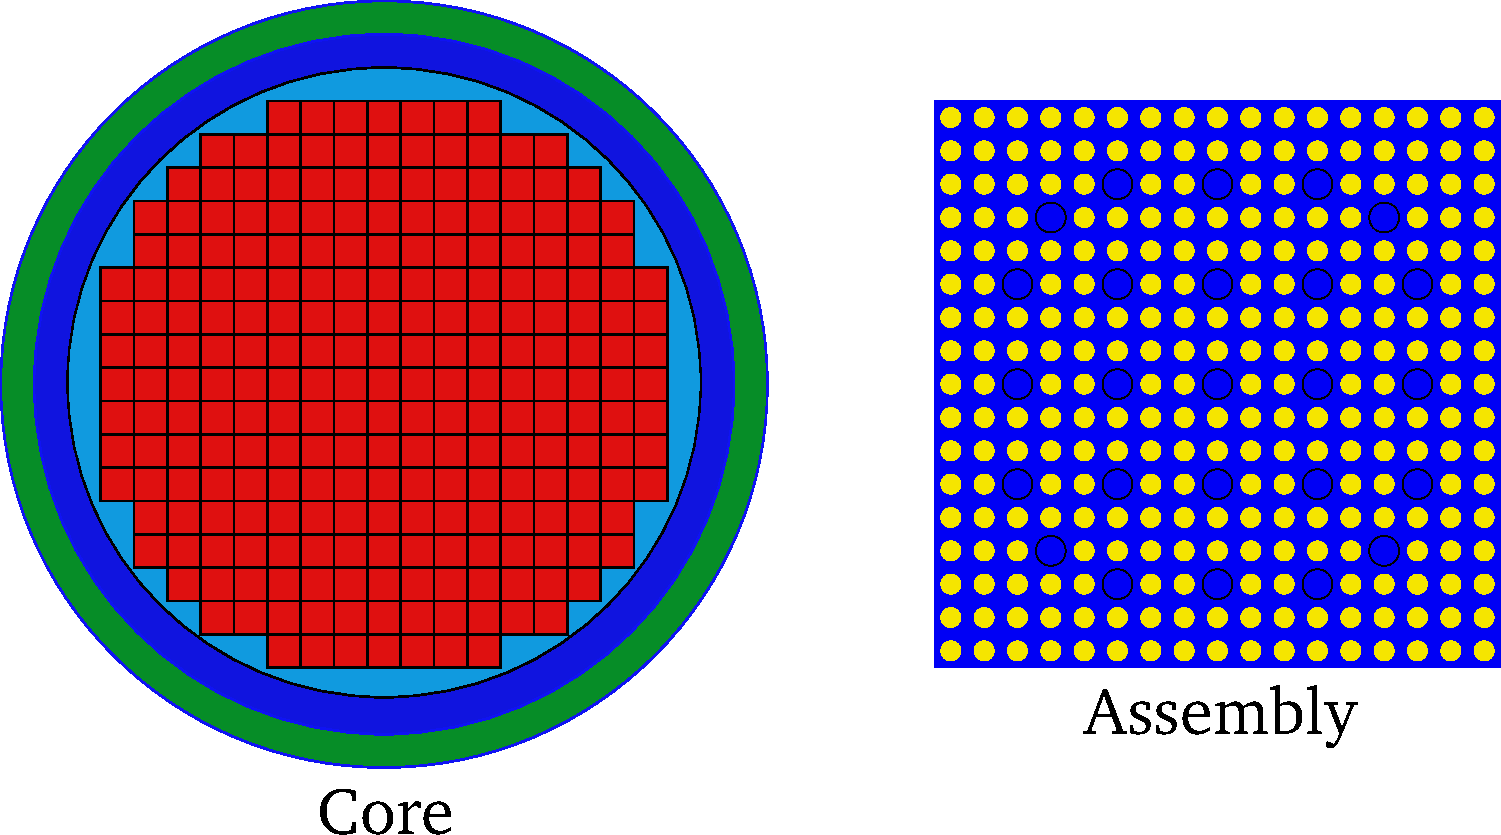
\includegraphics[width=5.0in]{figures/ch1/mcperformance.pdf}
  \caption{Geometry layout of the NEA Monte Carlo performance benchmark.}
  \label{fig:mcperformance}
\end{figure}

There are a number of simplifications in the Monte Carlo performance benchmark
model that make it quite unrealistic as far as light-water reactor (LWR) design
is concerned. There are no control rods, no core baffle, no grid spacers, and
very limited ex-core detail. Furthermore, the fact that all fuel pins are the
same enrichment and composition results in a roughly cosine distribution in the
axial direction and a Bessel distribution in the radial direction. All materials
in the problem are also specified to use cross sections at a single
temperature. Nevertheless, even this simplified problem is computationally
challenging due to the number of unknowns to be solved for. In this benchmark,
the aim is to compute the power distribution for every fuel pin subdivided into
100 evenly spaced axial nodes (note that the 10 radial rings per pin originally
specified by Smith were not included). With 264 fuel pins in each assembly and
241 assemblies, this means there are 6,362,400 unique regions that need to be
tallied over.

At the PHYSOR 2010 conference, Kelly et al. presented the first credible
solution to the Monte Carlo Performance benchmark \cite{physor-kelly-2010} using
the MC21 Monte Carlo code \cite{mc-sutton-2007} developed by the Knolls and
Bettis Atomic Power Laboratories. To solve for the local power distribution, a
simulation was run with 40 billion active neutron histories and the flux, total
absorption rate, and total fission rate were tallied over a pin cell mesh with
100 axial mesh cells. They faced a number of challenges and problems in their
solution:
\begin{itemize}
\item Even with 40 billion neutrons, virtually none of the local tallies had
  95\% confidence intervals with half-widths of less than 1\% of the mean as
  required by the Kord Smith Challenge.
\item Due to the highly non-uniform nature of the power distribution, regions of
  the problem with low fission rate density had correspondingly large variances.
\item Although the tallies in their simulation required about 0.5 GB of memory,
  the problem overall took over 6 GB. Since the SPMD method implies that all
  memory is replicated across different processes, the memory requirements could
  easily exceed that available on a single node. In their case, they had at
  least 24 GB of memory shared among four cores.
\item Since the benchmark model has a dominance ratio close to unity, Kelly et
  al. had to use 300 inactive batches before tallies even began to accumulate.
\end{itemize}
Their simulation ran for 18 hours on 400 processors, implying that on a single
processor it would have taken about 300 days.

Leppänen analyzed the Monte Carlo performance benchmark using the Serpent Monte
Carlo code \cite{vtt-leppanen-2007} and presented results at the SNA + MC2010
conference \cite{sna-leppanen-2010}. In his simulation, 100 billion active
neutron histories were used. Thanks to use of delta tracking and various methods
that enable a faster simulation at the expense of more memory in Serpent, the
simulation took about 21 days on 7 processor cores, a rate twice as fast as that
obtained in Kelly et al.'s 2010 analysis. No mention was made of the exact
memory requirements for the simulation.

At the PHYSOR 2012 conference, Kelly et al. gave an updated solution to the
Monte Carlo performance benchmark, again using MC21 but incorporating a few new
methods \cite{physor-kelly-2012}. The first modification was that they used
multiple fission generations per batch to eliminate the systematic
underprediction of confidence intervals. In addition, they introduced a new
methodology for weighting the fission source sites at each batch to achieve a
flatter variance distribution. With these two methods, they ran a simulation
with 200 billion active neutron histories and succeeded in reaching the
criterion of having 95\% of tallies with 95\% confidence intervals with half
widths of less than 1\% of their respective means. This simulation took 75.6
hours on 750 processor cores.

\subsection{MIT PWR Benchmark}

The introduction of the NEA Monte Carlo performance benchmark was an important
first step in encouraging the Monte Carlo community to start addressing problems
related to the ability to perform full-core simulations. The analyses by Kelly
et al. and Leppänen have shown that obtaining a solution is indeed possible
given the availability of large computing resources. However, as previously
mentioned, the benchmark model contains many model simplifications that make the
problem unrealistic.

To move towards simulation of actual reactor models, MIT is currently developing
a PWR full-core benchmark that includes details and dimensions from an actual
operating PWR plant. Many of the simplifications that were present in the NEA
Monte Carlo performance benchmark are not part of the MIT benchmark; features
that are explicitly modeled include radial enrichment zoning, guide tubes and
instrument tubes, burnable absorbers and control rods, grid spacers, core
support, core baffle, core barrel, thermal shield pads, and the reactor pressure
vessel. A geometry plot of the benchmark model is shown in
\autoref{fig:mit-pwr-benchmark}.
\begin{figure}[htb]
  \centering
  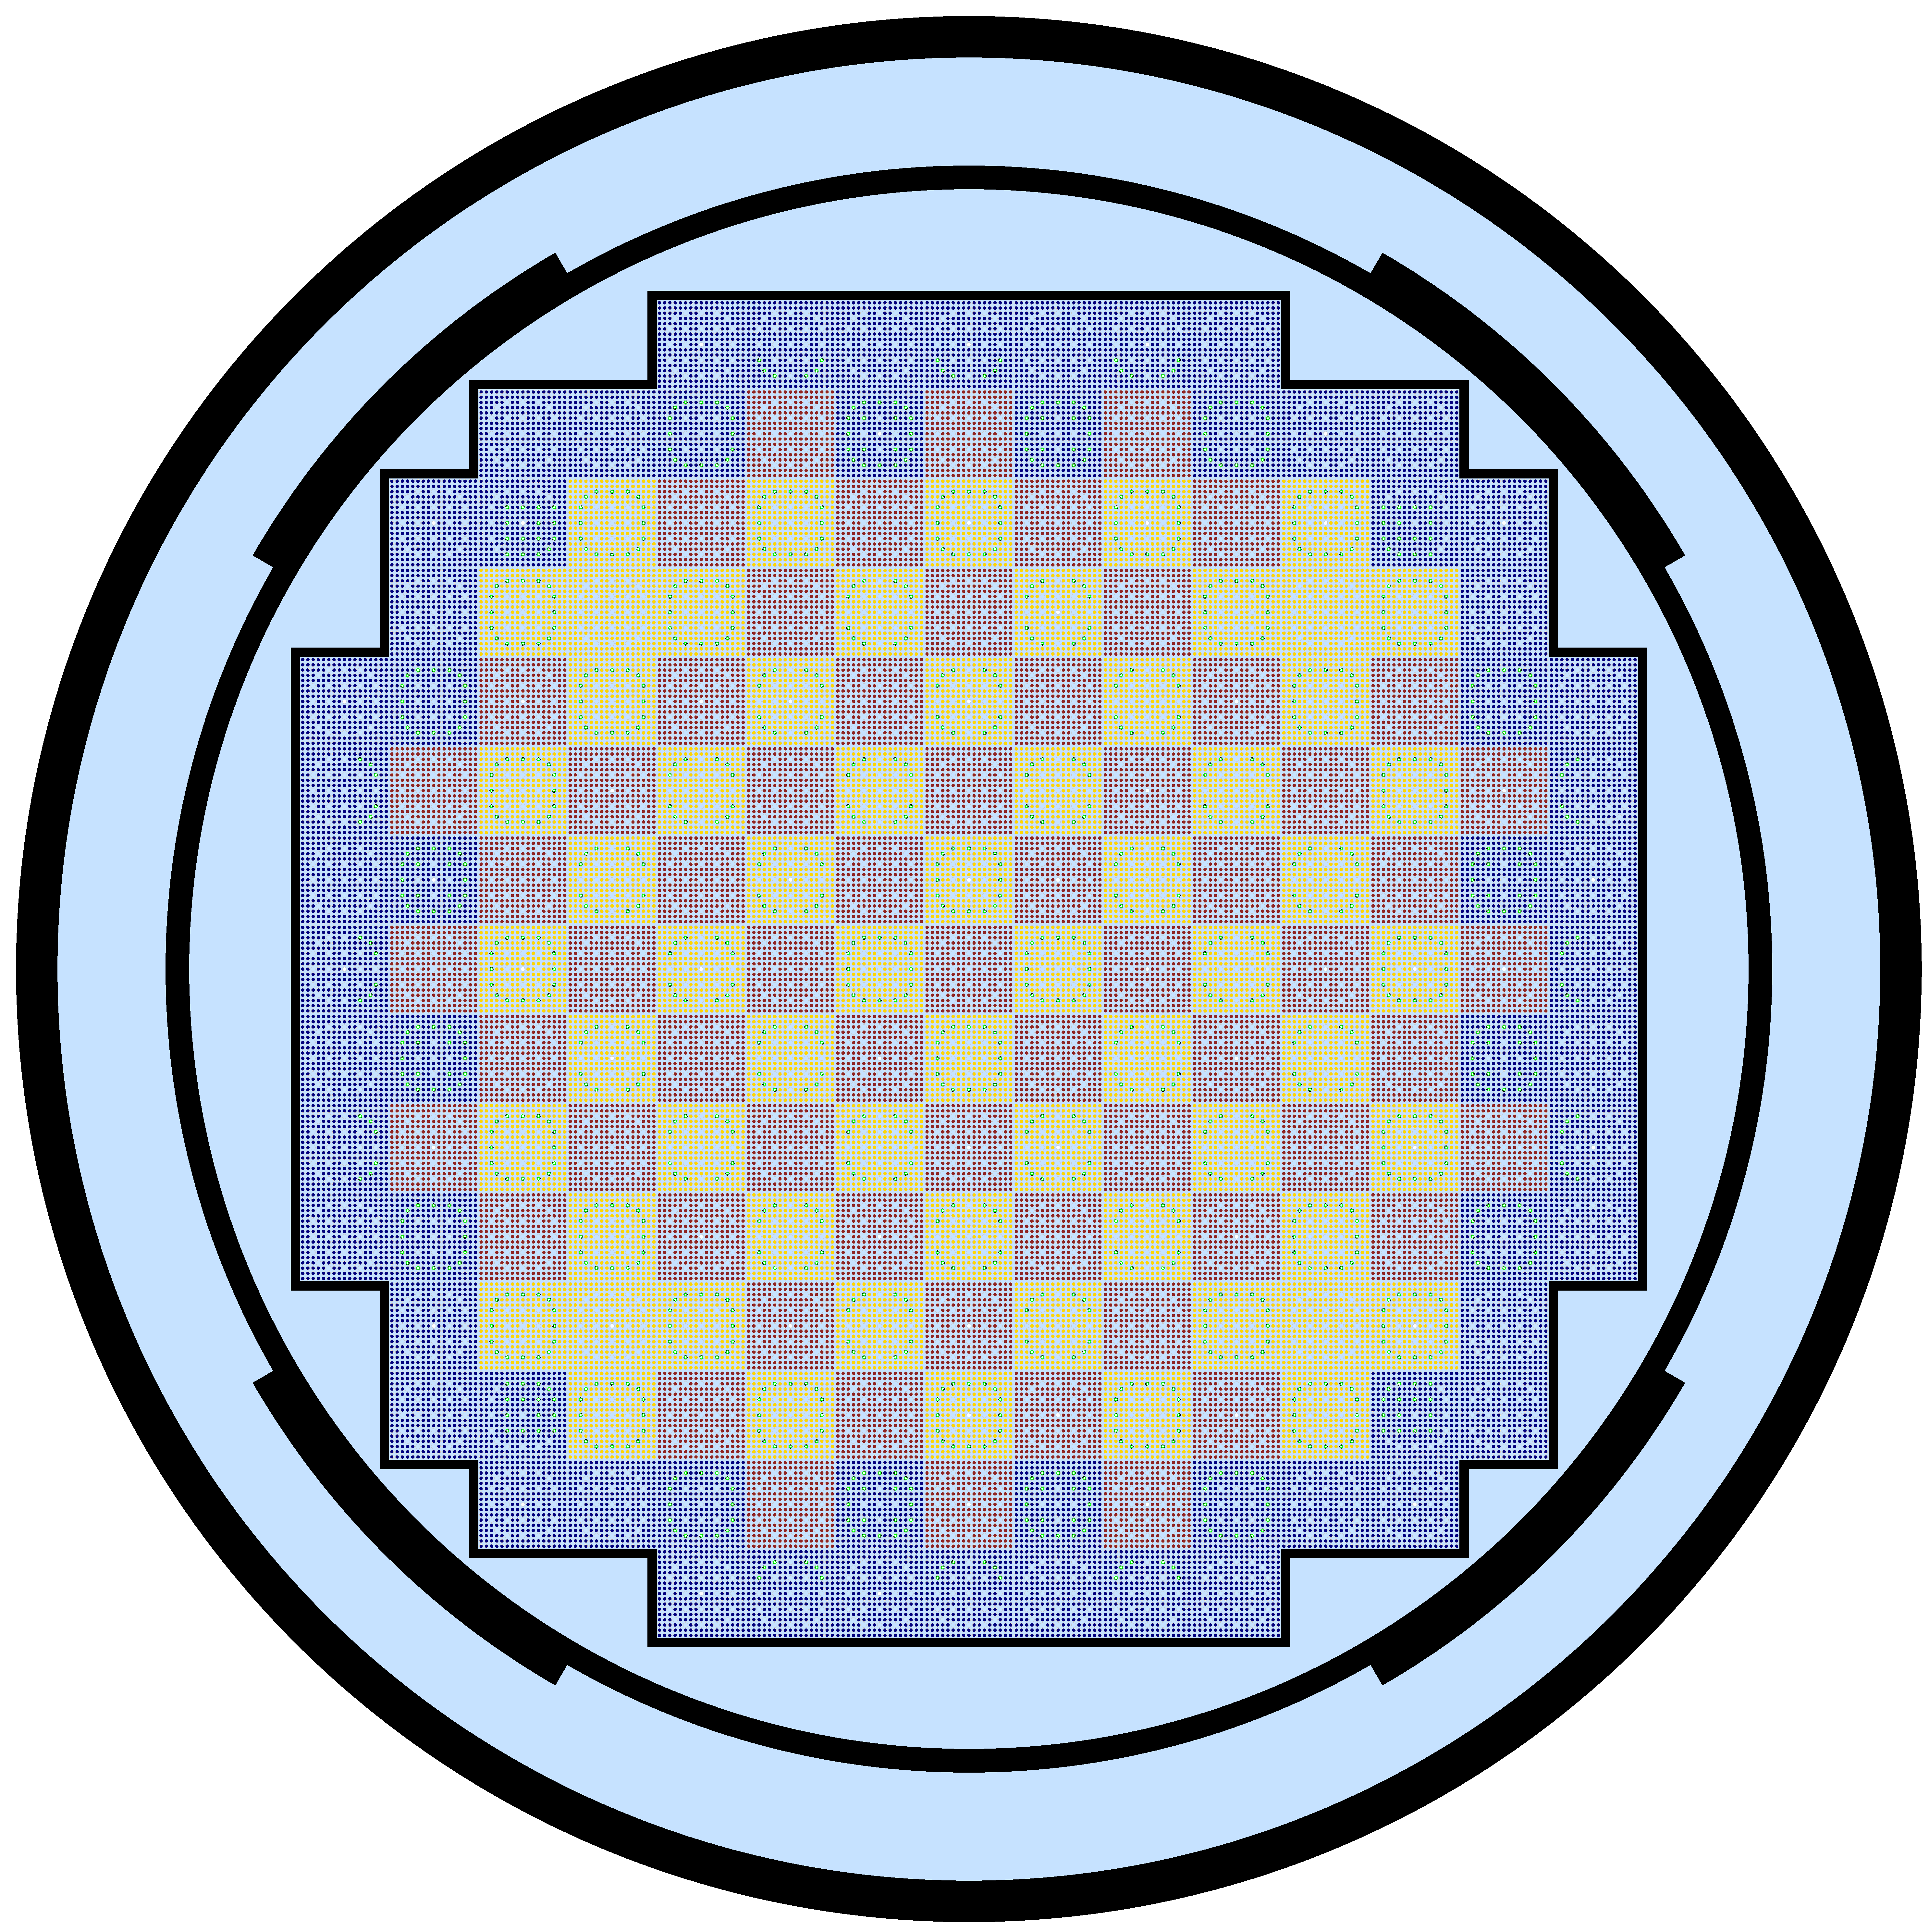
\includegraphics[width=4.0in]{figures/ch1/mit-pwr-benchmark.png}
  \caption{Geometry plot of a preliminary model of the MIT PWR Benchmark
    generated with the OpenMC Monte Carlo code.}
  \label{fig:mit-pwr-benchmark}
\end{figure}
The level of detail and complexity in the MIT benchmark will only exacerbate the
challenges encountered when simulating the Monte Carlo performance benchmark
including high memory requirements, poor source convergence, and the requirement
to run possibly trillions of particles to reach convergence of local tallies.

\section{Summary of Issues}

As we see from the preceding considerations, there are a number of formidable
challenges to simulating full-core reactor problems directly using Monte
Carlo. Perhaps the most important point to recognize (as it indirectly or
directly causes all other problems), is that to obtained a converged solution
for the spatial distribution of power in a full-core model will likely require
an unprecedented number of particle histories. The study of Kelly et
al. \cite{physor-kelly-2012} showed that even for the simplified NEA Monte Carlo
performance benchmark, 200 billion active neutron histories were required to
converge the local tallies. To accurately model changes in material compositions
due to depletion, it is likely that as many as 500 axial nodes will be required
instead of 100; on top of that, 10 radial rings per pin may be necessary. Thus,
assuming the number of particles needed to reach the desired uncertainty
criterion scales with the number of tally regions, we would need $200 \cdot 10^9
\times 5 \times 10 = 10 \cdot 10^{12}$, or ten trillion, neutrons to fully
converge all tallies.

Barring a huge increase in the efficiency of single processor cores, the
expedient solution of a full-core reactor problem will in turn require millions
of processors running simultaneously. To-date, only a few studies in the
literature have demonstrated the use of even thousands of processors in parallel
in a Monte Carlo neutron transport simulation \cite{lanl-brown-2005,
  ane-romano-2013}.

Let us now discuss each algorithmic issue in further detail to assess 1) whether
solutions to these problems already exist, 2) the status of current work towards
their resolution, and 3) what areas need further work. It is the last point that
motivates the objective of this thesis. 

\subsection{Source Convergence}

In a Monte Carlo $k$-eigenvalue calculation, we start with some assumed guess of
the actual fission source distribution. Before tallies can begin accumulating,
it is necessary to first iterate on the fission source to obtain a converged
distribution. The rate at which the fission source distribution will converge
depends on a quantity known as the \emph{dominance ratio}, the ratio of the
first higher harmonic eigenvalue to the fundamental mode eigenvalue. The closer
the dominance ratio is to one, the more difficult it is to converge the fission
source distribution.

In a typical commercial light-water reactor, the width and height of the reactor
core are very large relative to the mean free path of neutrons. As a result,
full-core reactor models typically have dominance ratios close to
unity. Converging on the fission source distribution can consequently require
hundreds of iterations if using standard power iteration. With a small batch
size, this might not be much of a concern. However, in a simulation with
possibly millions of processor cores, each one must be occupied with sufficient
work. As a result, batch sizes with many billions of particles would be needed
in practice. If we are to discard hundreds of batches, each composed of billions
of particles, at the beginning of every simulation, a great amount of processor
time may be wasted.

A number of solutions have been proposed to obtain faster fission source
convergence in Monte Carlo $k$-eigenvalue calculations. These include the
fission matrix method \cite{ane-dufek-2007, lanl-carney-2012}, Wielandt's method
\cite{jnst-yamamoto-2004, mc-brown-2007}, extrapolation methods
\cite{mc-toth-2007-1, mc-toth-2007-2}, and acceleration via low-order operators
(e.g. coarse mesh finite difference \cite{physor-lee-2010, sna-lee-2010,
  physor-lee-2012}), to name a few. Lee et al. \cite{physor-lee-2012} have
demonstrated that the CMFD formulation can reduce the number of inactive batches
in an eigenvalue calculation to less than 20 with effectively no overhead from
solving the low-order CMFD system. With this and other viable solutions at hand,
source convergence is now considered by many in the Monte Carlo community to be
a solved problem. Methods to accelerate fission source convergence have been or
are currently being implemented in a number of Monte Carlo codes including MCNP
\cite{lanl-young-2011}, MC21, and OpenMC \cite{mc-romano-2013}.

While source convergence may now be of less concern than it was years ago thanks
to effective acceleration methods, the diagnosis and suppression of tally bias
due to undersampling \cite{nse-ueki-2005, nse-ueki-2008, jnst-ueki-2011} is
still an outstanding problem. However, this is primarily a physics problem that
will not impede the successful implementation of scalable parallel
algorithms. As such, it is not explored in this thesis.

\subsection{Cross Section Memory Requirements}
\label{sec:cross-section-memory}

One of the simplifications in the NEA Monte Carlo performance benchmark is that
all materials are to be treated at the same temperature. This was done for
practical purposes as it allows someone simulating the benchmark to use cross
section data processed at a single temperature (in this case room
temperature). However, for problems containing nuclides at many temperatures
(e.g. a reactor at full power), or with time-varying temperatures, it is
necessary to store cross sections at many temperatures.

The next natural question is then --- how many temperatures are necessary? This
question was studied in some depth by Trumbull \cite{nt-trumbull-2006}. He
concluded that for many nuclides, cross sections would need to be stored at
increments of less than 28 K. Assuming that even a 28 K interval were
sufficient, this means that over the range of temperatures found in a
light-water reactor (typically 293 K up to at least 1300 K for steady state
calculations and 2500 K for transients), cross sections would be needed at over
75 different temperatures. Thus, potentially hundreds of GB of memory are needed
to accommodate cross sections for a truly temperature-dependent model. The
reader should once again recall that, in the standard SPMD parallel model, this
memory requirement is to be multiplied by the number of processes used in the
simulation. It is thus anticipated that special techniques will need to be
employed in order to perform massively-parallel full-core LWR simulations given
that the memory requirements will almost certainly exceed the available node
memory.

Two solutions for reducing cross section memory requirements have thus far been
proposed. The first method is known as on-the-fly Doppler broadening
\cite{nse-yesilyurt-2012, trans-brown-2012}. The basic idea is that the cross
section at any temperature can be represented as a series expansion. As a
result, only the 0 K cross sections and a series of expansion coefficients need
be stored in memory. While this method does show some promise, it may not
ultimately be an adequate solution for LWR simulation since the range of
temperatures and required accuracy could necessitate that the series expansion
contain at least 13 terms and possibly more for certain nuclides
\cite{net-martin-2012}. Thus, the problem is merely shifted from storing cross
sections at a multitude of temperatures to storing a multitude of series
expansion coefficients.

Another method that may potentially solve the cross section memory requirements
is the work of Viitanen on explicit temperature treatment
\cite{nse-viitanen-2012, physor-viitanen-2012}. This method would enable
simulation using 0 K cross sections via a rejection technique based on Woodcock
delta tracking. The downside is that the method may incur a performance
penalty. However, from the perspective of massively parallel simulations, the
trade-off of a slower calculational rate in return for drastically reduced
memory requirement is quite tolerable. It is often said that ``flops are free''
\cite{sc-panel-2009}; on the other hand, memory is an increasingly scarce
resource for high fidelity simulations. Given that excellent progress has been
made towards reducing cross section memory requirements, it is a topic that will
not be further explored as part of the current work.

\subsection{Tally Memory Requirements}
\label{sec:tally-memory}

Kelly et al. \cite{physor-kelly-2012} found that the memory required in their
simulation of the Monte Carlo performance benchmark was so large that they were
unable to use all processors on a single node. For that problem, the tallies
consumed about 0.5 GB on each process --- a number that actually may not, at
first glance, seem that prohibitive. However, we must keep in mind the following
facts: 1) they were only solving for a few (three) physical quantities for each
tally region, and 2) the number of regions they used may be 50 times smaller
than that needed for a realistic reactor simulation.

If we were really only interested in a steady-state problem, it would suffice to
calculate just the total energy deposition in each tally region and perhaps a
few more quantities. However, the fuel composition will slowly change over time
due to irradiation and depletion of the fuel. Furthermore, while fresh fuel in a
reactor may be composed of only a few nuclides, over time hundreds of actinides
and fission product nuclides will appear in the fuel due to nuclear
transmutation. This process is governed by a set of equations called the Bateman
equations \cite{ane-cetnar-2006}. In order to solve the Bateman equations, one
needs to know various reaction rates in each nuclide in the fuel: the fission
reaction rate, the $(n,\gamma)$ reaction rate, the $(n,2n)$ reaction rate, the
$(n,3n)$ reaction rate, the $(n,\alpha)$ reaction rate, and the $(n,p)$ reaction
rate.

To get an idea for just how large the memory requirements for tallies might be,
let us consider a depletion simulation of the MIT PWR benchmark. This benchmark
has 193 assemblies, each having 264 pins. With 500 axial and 10 radial zones
within each fuel pin for depletion purposes, the total number of depletable
materials would be 254,760,000. With approximately 300 nuclides and six reaction
rates needed for each nuclide, the total memory for tallies would be
$254,760,000 \times 300 \times 6 \times 24 \text{ bytes} = 11,005,632,000,000$
bytes\footnote{We have chosen the last multiplier as 24 bytes for the following
  reason; for each tally bin we need to store the accumulated sum, the
  accumulated sum of squares, and also a temporary variable that is used for a
  single batch. Thus there are three 8-byte floating point numbers.} or
\textbf{11 terabytes}. Again, in the SPMD parallel model, this amount of memory
would be required for each process. This is clearly a major problem and one that
has no easy resolution.

One of the primary objectives of this thesis is to study algorithms for
decomposing tally memory and provide guidance on the best path going forward for
realistic LWR analysis. Two classes of strategies have been proposed to address
this problem --- what we loosely refer to as \emph{data decomposition} and
\emph{domain decomposition}. Data decomposition could take many forms, but the
basic approach would involve the same naturally parallel by-particle
parallelization strategy as is currently employed together with a set of
dedicated \emph{tally servers} that continuously receive tally updates from the
tracking processors (e.g. with one-side operations or by running a continuous
receive loop). The spatial decomposition of the tallies is in general arbitrary
and the data sent from the tracking processors could be carried out with
non-blocking MPI send operations to maximize overlap in
communication/computation.

Domain decomposition on the other hand associates a contiguous region of
physical space with each processing element (or node). Each processor then owns
the subset of tallies for the corresponding region of physical space. This
approach is potentially made efficient with a more complex parallelization
strategy where each processor only tracks the particles that are passing through
its own portion of the domain.  However, new complexities emerge --- fast
neutrons travel long distances before absorption, and thus the local leakage
rates (probability of a neutron leaving a partition before being absorbed) are
relatively large. This requires intermediate data exchange \emph{stages} where
particles are moved to adjacent processors, potentially leading to significant
communication costs and non-trivial load imbalances.

\subsection{Degradation of Parallel Efficiency}

Thus far, we have discussed algorithmic problems that arise when simulating
full-core reactor models, regardless of how many processors are utilized. The
full-core LWR simulations that have been performed to date
\cite{sna-leppanen-2010, physor-kelly-2012} have generally used under 1000
processors. With this many processors, overhead from network communication is
generally small compared to the overall computation time, especially when using
a high-speed network interconnect. However, more realistic reactor simulations
will require trillions of particles and hence orders of magnitude greater
processor core counts. That being the case, the network communication from
message-passing can quickly become prohibitive if scalable algorithms are not
utilized. Until recently, Monte Carlo particle transport simulations using this
many processors had not been attempted --- in fact, the first attempts at such
large runs are presented in this thesis.

It has been fairly well-documented that current production Monte Carlo codes,
such as MCNP \cite{nt-goorley-2012}, do not scale well to large numbers of
processors. So bad is the problem that a prominent researcher has recently
questioned whether Monte Carlo truly ``is ... embarrassingly parallel''
\cite{physor-hoogenboom-2012}. The inability to achieve scaling can be traced to
one fundamental design flaw. Most parallel algorithms in Monte Carlo codes are
commonly implemented in the form of a \emph{master-slave} algorithms. This means
that one process acts as the \emph{master}, assigning and coordinating work
between all other \emph{slave} processes. While master-slave algorithms can be
beneficial from the perspective of maintaining good load balancing, they can
also unfortunately create a bottleneck at the master process. In practice, poor
scaling can result from two distinct algorithms:
\begin{enumerate}
\item \emph{Fission source synchronization} --- in an eigenvalue calculation, it
  is necessary to iterate over the fission source to obtain a converged
  distribution. During each fission source iteration, source sites are generated
  as fission occurs and are stored in an array called the \emph{fission
    bank}. As the generation of these sites is stochastic, we may end up with
  fewer or more sites than particles requested per source iteration. Thus the
  specified number of sites must be sampled from the fission bank. Common
  implementations rely on a single master processor to
  sort/re-order\footnote{This is done for the sake of maintaining
    reproducibility, which is discussed at length in
    \autoref{chap:fission-bank}.}, sample, and redistribute all source sites.
\item \emph{Tally reduction} --- in many Monte Carlo codes, each process
  responsible for tracking particles accumulates its own estimates of the tally
  random variables. At the end of every realization, these estimates are added
  together to obtain a single estimate (with lower variance). In terms of
  network communication, this requires that the tallies be \emph{reduced} from
  all processors to one, a process which can take $O(p \log_2 p)$ steps where
  $p$ is the number of processes. This generally affects both fixed source and
  eigenvalue calculations, but is only a problem when many tally bins are
  used. We saw earlier that for realistic reactor calculations, terabytes of
  memory corresponding to many billions of tally bins would be necessary.
\end{enumerate}
For the time being, we will defer further discussion regarding these algorithms
to the chapters where they are analyzed thoroughly. However, we remark that not
only are these problems unsolved, they are not even widely recognized by many in
the community. A major objective of this thesis will be to propose, analyze, and
demonstrate scalable algorithms for tally reduction and fission source
synchronization.

\section{Objectives}

The preceding summary identified a number of challenges that must be overcome
before Monte Carlo simulation of full-core light-water reactors is
possible. While some of these challenges have either been solved or are
currently being researched substantially elsewhere, other areas have received
very little attention. The major objectives of this thesis are threefold:
\begin{enumerate}
\item To demonstrate a method for collecting tally results without massive
  network communication that erodes scalability for large tallies and processor
  counts;
\item To analyze and implement a nearest-neighbor algorithm for sampling and
  distributing source sites in $k$-eigenvalue calculations; and
\item To study algorithms for decomposing tally memory in light-water reactor
  simulations, namely domain decomposition and data decomposition, and evaluate
  the inherent trade-offs.
\end{enumerate}

The studies and results being presented here would not have been possible
without a substantial level of code development within a production Monte Carlo
code that employs realistic geometry and physics models. Unfortunately, many
production Monte Carlo codes that are widely used in the community, such as MCNP
and KENO \cite{ornl-petrie-1990}, have a long legacy attached to them and are
not written using modern programming paradigms. This, combined with the
complexity of these codes, often makes them ill-suited for research purposes. As
part of the present work, a modern, high-performance, extensible, open source
Monte Carlo code called OpenMC has been developed and released to the
public. The development and methodology of the OpenMC Monte Carlo code is
discussed thoroughly in \autoref{chap:openmc}.

In \autoref{chap:fission-bank}, we present a theoretical analysis of both the
traditional parallel fission bank algorithm used in Monte Carlo eigenvalue
calculations as well as a novel algorithm based on nearest-neighbor exchanges of
source sites. The novel algorithm is implemented in the OpenMC Monte Carlo code
and tested to validate the theoretical analysis. Finally, possible concerns
including load balancing, ordering of the fission bank, and fault tolerance are
discussed.

In \autoref{chap:tally-reduction}, we begin by demonstrating why reducing
tallies at every realization during a Monte Carlo simulation may incur
significant network communication. A means of reducing communication by using
the concept of \emph{batching} is proposed and compared to techniques used to
eliminate correlation between successive realizations in eigenvalue
calculations. The method is implemented in OpenMC, tested on a problem with
large tallies, and demonstrated to reduce communication substantially.

In \autoref{chap:domain-decomp}, a model is developed to predict the impact of
particle load imbalances on the performance of domain decomposition algorithms
for Monte Carlo neutron transport, specifically as applied to LWR
analysis. Expressions for upper bound performance ``penalties'' are derived in
terms of simple machine characteristics, material characterizations, and initial
particle distributions. Important limitations for domain decomposed simulations
are identified and discussed based on the upper bound penalties.

In \autoref{chap:data-decomp}, an algorithm for decomposing large tally data in
Monte Carlo particle simulations is developed, analyzed and implemented in
OpenMC. The algorithm is based on a non-overlapping decomposition of compute
nodes into tracking processors and tally servers. The former are used to
simulate the movement of particles through the domain while the latter
continuously receive and update tally data. A performance model for this
approach is developed, showing that, for a range of parameters relevant to LWR
analysis, the tally server algorithm should perform with minimal overhead on
contemporary supercomputers. An implementation of the algorithm in OpenMC is
then tested on the Intrepid and Titan supercomputers, supporting the key
predictions of the model over a wide range of parameters.

\chapter{The OpenMC Monte Carlo Code}
\label{chap:openmc}

\section{Background}

As part of the present work, a general Monte Carlo neutron transport code was
written from scratch with an emphasis on high performance algorithms, accurate
physics capabilities, and modern software design practices. The development of
the code started as a simplistic platform, first mentioned in
\cite{lanl-romano-2009}, within which algorithms could be easily tested. At that
stage, the geometry was limited to a simple structured mesh and all physics were
based on predefined fictitious multigroup cross-sections. However, as further
studies of domain and data decomposition schemes, described in
\autoref{chap:domain-decomp} and \autoref{chap:data-decomp}, demanded that
realistic geometry and physics be present, a decision was made to greatly expand
the capabilities of the code.

In early 2011, the geometry and physics from the original structured-mesh,
multigroup code was gutted and replaced with constructive solid geometry
routines and physics based on continuous-energy cross sections. In Fall 2011,
the input file format was changed to an XML format and a basic outline of the
current tally system was introduced. Since then, improvements have been made in
physics methods, geometry capabilities, and input/output options.

OpenMC has been described in a recent paper in \emph{Annals of Nuclear Energy}
\cite{ane-romano-2013}. Further developments will be reported in a paper at the
M\&C 2013 conference \cite{mc-romano-2013}.

\section{Overview of Program Flow}

OpenMC performs a Monte Carlo simulation one particle at a time --- at no point
is more than one particle being tracked on a single program instance. Before any
particles are tracked, the problem must be initialized. This involves the
following steps:
\begin{itemize}
\item Read input files and build data structures for the geometry, materials,
  tallies, and other associated variables.
\item Initialize the pseudorandom number generator.
\item Read ACE format cross-sections specified in the problem.
\item If using a special energy grid treatment such as a union energy grid with
  pointers, that must be initialized as well.
\item In a fixed source problem, source sites are sampled from the specified
  source. In an eigenvalue problem, source sites are sampled from some initial
  source distribution or from a source file. The source sites consist of
  coordinates, a direction, and an energy.
\end{itemize}
Once initialization is complete, the actual transport simulation can
proceed. The life of a single particle will proceed as follows:
\begin{enumerate}
\item The particle's properties are initialized from a source site previously
  sampled.
\item Based on the particle's coordinates, the current cell in which the
  particle resides is determined.
\item The energy-dependent cross-sections for the material that the particle is
  currently in are determined. Note that this includes the total cross-section,
  which is not pre-calculated.
\item The distance to the nearest boundary of the particle's cell is determined
  based on the bounding surfaces to the cell.
\item The distance to the next collision is sampled. If the total material
  cross-section is $\Sigma_t$, this can be shown to be
  \begin{equation}
    d = -\frac{\ln \xi}{\Sigma_t}
  \end{equation}
  where $\xi$ is a pseudorandom number sampled from a uniform distribution on
  $[0,1)$.
\item If the distance to the nearest boundary is less than the distance to the
  next collision, the particle is moved forward to this boundary. Then, the
  process is repeated from step 2. If the distance to collision is closer than
  the distance to the nearest boundary, then the particle will undergo a
  collision.
\item The material at the collision site may consist of multiple
  nuclides. First, the nuclide with which the collision will happen is sampled
  based on the total cross-sections. If the total cross section of material $i$
  is $\Sigma_{t,i}$, then the probability that any nuclide is sampled is
  \begin{equation}
    P(i) = \frac{\Sigma_{t,i}}{\Sigma_t}.
  \end{equation}
\item Once the specific nuclide is sampled, the random samples a reaction for
  that nuclide based on the microscopic cross sections. If the microscopic
  cross-section for some reaction $x$ is $\sigma_x$ and the total microscopic
  cross section for the nuclide is $\sigma_t$, then the probability that
  reaction $x$ will occur is
  \begin{equation}
    P(x) = \frac{\sigma_x}{\sigma_t}.
  \end{equation}
\item If the sampled reaction is elastic or inelastic scattering, the outgoing
  energy and angle is sampled from the appropriate distribution.  If the
  reaction is $(n,xn)$, it's also treated as scattering and the weight of the
  particle is increased by the multiplicity of the reaction. The particle then
  continues from step 3. If the reaction is absorption or fission, the particle
  dies and if necessary, fission sites are created and stored in the fission
  bank.
\end{enumerate}
After all particles have been simulated, there are a few final tasks that must
be performed before the run is finished. This include the following:
\begin{itemize}
\item With the accumulated sum and sum of squares for each tally, the sample
  mean and its variance is calculated.
\item All tallies and other results are written to disk.
\item If requested, a source file is written to disk
\item All allocatable arrays are deallocated.
\end{itemize}

\section{Geometry}

\subsection{Constructive Solid Geometry}

OpenMC uses a technique known as constructive solid geometry (CSG) to build
arbitrarily complex three-dimensional models in Euclidean space. In a CSG model,
every unique object is described as the union, intersection, or difference of
\emph{half-spaces} created by bounding surfaces. Every surface divides all of
space into exactly two half-spaces. We can mathematically define a surface as a
collection of points that satisfy an equation of the form $f(x,y,z) = 0$ where
$f(x,y,z)$ is a given function. All coordinates for which $f(x,y,z) < 0$ are
referred to as the negative half-space (or simply the \emph{negative side}) and
coordinates for which $f(x,y,z) > 0$ are referred to as the positive half-space.

Let us take the example of a sphere centered at the point $(x_0,y_0,z_0)$
with radius $R$. One would normally write the equation of the sphere as
\begin{equation}
  \label{eq:sphere-equation}
  (x - x_0)^2 + (y - y_0)^2 + (z - z_0)^2 = R^2.
\end{equation}
By subtracting the right-hand term from both sides of
\eqref{eq:sphere-equation}, we can then write the surface equation for the
sphere:
\begin{equation}
  \label{eq:surface-equation-sphere}
  f(x,y,z) = (x - x_0)^2 + (y - y_0)^2 + (z - z_0)^2 - R^2 = 0
\end{equation}
One can confirm that any point inside this sphere will correspond to
$f(x,y,z) < 0$ and any point outside the sphere will correspond to
$f(x,y,z) > 0$.

In OpenMC, every surface defined by the user is assigned an integer to uniquely
identify it. We can then refer to either of the two half-spaces created by a
surface by a combination of the unique ID of the surface and a positive/negative
sign. For example, to refer to the negative half-space of a sphere (the volume
inside the sphere) with unique ID 35, the reference would be
-35. \autoref{fig:halfspace} shows an example of an ellipse with unique ID 1
dividing space into two half-spaces.
\begin{figure}[htb]
  \centering
  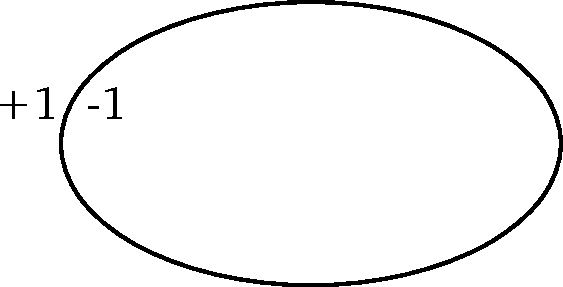
\includegraphics[width=3.0in]{figures/ch2/halfspace.pdf}
  \caption{Example of an ellipse and its associated half-spaces.}
  \label{fig:halfspace}
\end{figure}

References to half-spaces created by surfaces are used to define regions of
space of uniform composition, known as \emph{cells}. While some codes allow
regions to be defined by intersections, unions, and differences or half-spaces,
OpenMC is currently limited to cells defined only as intersections of
half-spaces. Thus, the specification of the cell must include a list of
half-space references whose intersection defines the region. The region is then
assigned a material defined elsewhere. \autoref{fig:union} shows an example of a
cell defined as the intersection of an ellipse and two planes.
\begin{figure}[htb]
  \centering
  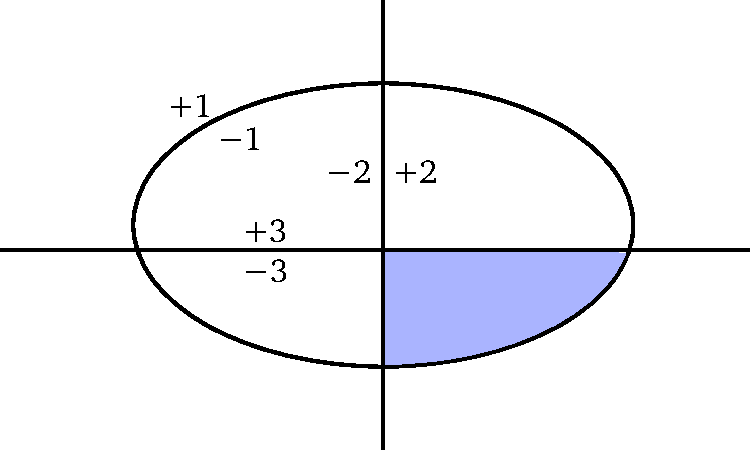
\includegraphics[width=4.0in]{figures/ch2/union.pdf}
  \caption{The shaded region represents a cell bounded by three surfaces.}
  \label{fig:union}
\end{figure}

The ability to form regions based on bounding quadratic surfaces enables OpenMC
to model arbitrarily complex three-dimensional objects. In practice, one is
limited only by the different surface types available in
OpenMC. \autoref{tab:surfaces} lists the available surface types, the identifier
used to specify them in input files, the corresponding surface equation, and the
input parameters needed to fully define the surface.
\begin{table}[htb]
  \caption{Surface types available in OpenMC.}
  \label{tab:surfaces}
  \footnotesize{
  \begin{tabular}{c c c c}
    \toprule
    Surface & Identifier & Equation & Parameters \\
    \midrule
    Plane perpendicular to $x$-axis & x-plane & $x - x_0 = 0$ & $x_0$ \\

    Plane perpendicular to $y$-axis & y-plane & $y - y_0 = 0$ & $y_0$ \\

    Plane perpendicular to $z$-axis & z-plane & $z - z_0 = 0$ & $z_0$ \\

    Arbitrary plane & plane & $Ax + By + Cy = D$ & $A \; B \; C \; D$ \\

    Infinite cylinder parallel to $x$-axis & x-cylinder & $(y - y_0)^2 + (z -
    z_0)^2 = R^2$ & $y_0 \; z_0 \; R$ \\

    Infinite cylinder parallel to $y$-axis & y-cylinder & $(x - x_0)^2 + (z -
    z_0)^2 = R^2$ & $x_0 \; z_0 \; R$ \\

    Infinite cylinder parallel to $z$-axis & z-cylinder & $(x - x_0)^2 + (y -
    y_0)^2 = R^2$ & $x_0 \; y_0 \; R$ \\

    Sphere & sphere & $(x - x_0)^2 + (y - y_0)^2 + (z - z_0)^2 = R^2$ & $x_0 \;
    y_0 \; z_0 \; R$ \\

    Cone parallel to the $x$-axis & x-cone & $(y - y_0)^2 + (z - z_0)^2 = R^2(x
    - x_0)^2 $ & $x_0 \; y_0 \; z_0 \; R^2$ \\

    Cone parallel to the $y$-axis & y-cone & $(x - x_0)^2 + (z - z_0)^2 = R^2(y
    - y_0)^2 $ & $x_0 \; y_0 \; z_0 \; R^2$ \\

    Cone parallel to the $z$-axis & z-cone & $(x - x_0)^2 + (y - y_0)^2 = R^2(z
    - z_0)^2 $ & $x_0 \; y_0 \; z_0 \; R^2$ \\

    \bottomrule
  \end{tabular}
  }
\end{table}

\subsubsection{Universes}

OpenMC supports universe-based geometry similar to the likes of MCNP
\cite{lanl-x5-2008} and Serpent \cite{vtt-leppanen-2007}. This capability
enables users to model any identical repeated structures once and then fill them
in various spots in the geometry. A prototypical example of a repeated structure
would be a fuel pin within a fuel assembly or a fuel assembly within a core.

Each cell in OpenMC can either be filled with a normal material or with a
universe. If the cell is filled with a universe, only the region of the universe
that is within the defined boundaries of the parent cell will be present in the
geometry. That is to say, even though a collection of cells in a universe may
extend to infinity, not all of the universe will be ``visible'' in the geometry
since it will be truncated by the boundaries of the cell that contains it.

When a cell is filled with a universe, it is possible to specify that the
universe filling the cell should be rotated and translated. This is done through
the \texttt{rotation} and \texttt{translation} attributes on a cell (note though
that these can only be specified on a cell that is filled with another universe,
not a material).

It is not necessary to use or assign universes in a geometry if there are no
repeated structures. Any cell in the geometry that is not assigned to a
specified universe is automatically part of the \emph{base universe} whose
coordinates are just the normal coordinates in Euclidean space.

\subsubsection{Lattices}

Often times, repeated structures in a geometry occur in a regular pattern such
as a rectangular or hexagonal lattice. In such a case, it would be cumbersome
for a user to have to define the boundaries of each of the cells to be filled
with a universe. Thus, OpenMC provides a lattice capability similar to that used
in MCNP and Serpent.

The implementation of lattices is similar in principle to universes --- instead
of a cell being filled with a universe, the user can specify that it is filled
with a finite lattice. The lattice is then defined by a two-dimensional array of
universes that are to fill each position in the lattice. A good example of the
use of lattices and universes can be seen in the OpenMC model for the Monte
Carlo Performance benchmark \cite{romano-2012}.

\subsection{Computing the Distance to Nearest Boundary}

One of the most basic algorithms in any Monte Carlo code is determining the
distance to the nearest surface within a cell. Since each cell is defined by
the surfaces that bound it, if we compute the distance to all surfaces bounding
a cell, we can determine the nearest one.

With the possibility of a particle having coordinates on multiple levels
(universes) in a geometry, we must exercise care when calculating the distance
to the nearest surface. Each different level of geometry has a set of boundaries
with which the particle's direction of travel may intersect. Thus, it is
necessary to check the distance to the surfaces bounding the cell in each
level. This should be done starting the highest (most global) level going down
to the lowest (most local) level. That ensures that if two surfaces on different
levels are coincident, by default the one on the higher level will be selected
as the nearest surface. Although they are not explicitly defined, it is also
necessary to check the distance to surfaces representing lattice boundaries if a
lattice exists on a given level.

The following procedure is used to calculate the distance to each bounding
surface. Suppose we have a particle at $(x_0,y_0,z_0)$ traveling in the
direction $u_0,v_0,w_0$. To find the distance $d$ to a surface $f(x,y,z) = 0$,
we need to solve the equation:
\begin{equation}
  \label{eq:dist-to-boundary-1}
  f(x_0 + du_0, y + dv_0, z + dw_0) = 0.
\end{equation}
Since $f(x,y,z)$ in general is quadratic in $x$, $y$, and $z$, this implies that
$f(x_0 + du_0, y + dv_0, z + dw_0)$ is quadratic in $d$. Thus we expect at most
two real solutions to \eqref{eq:dist-to-boundary-1}. If no solutions to
\eqref{eq:dist-to-boundary-1} exist or the only solutions are complex, then the
particle's direction of travel will not intersect the surface. If the solution
to \eqref{eq:dist-to-boundary-1} is negative, this means that the surface is
``behind'' the particle, i.e. if the particle continues traveling in its current
direction, it will not hit the surface.

Once a distance has been computed to a surface, we need to check if it is closer
than previously-computed distances to surfaces. Unfortunately, we cannot just
use the minimum function because some of the calculated distances, which should
be the same in theory (e.g. coincident surfaces), may be slightly different due
to the use of floating-point arithmetic. Consequently, we should first check for
floating-point equality of the current distance calculated and the minimum found
thus far. This is done by checking if
\begin{equation}
  \label{eq:fp-distance}
  \frac{| d - d_{min} |}{d_{min}} < \epsilon
\end{equation}
where $d$ is the distance to a surface just calculated, $d_{min}$ is
the minimum distance found thus far, and $\epsilon$ is a small number. In
OpenMC, this parameter is set to $\epsilon = 10^{-14}$ since all floating
calculations are done on 8-byte floating point numbers.

\subsection{Finding a Cell Given a Point}
\label{sec:find-cell}

Another basic algorithm is to determine which cell contains a given point in the
global coordinate system, i.e. if the particle's position is $(x,y,z)$, what
cell is it currently in. This is done in the following manner in OpenMC. With
the possibility of multiple levels of coordinates, we must perform a recursive
search for the cell. First, we start in the highest (most global) universe,
which we call the base universe, and loop over each cell within that
universe. For each cell, we check whether the specified point is inside the cell
using the algorithm described in \autoref{sec:cell-contains}. If the cell is
filled with a normal material, the search is done and we have identified the
cell containing the point. If the cell is filled with another universe, we then
search all cells within that universe to see if any of them contain the
specified point. If the cell is filled with a lattice, the position within the
lattice is determined, and then whatever universe fills that lattice position is
recursively searched. The search ends once a cell containing a normal material
is found that contains the specified point.

\subsection{Determining if a Coordinate is in a Cell}
\label{sec:cell-contains}

To determine which cell a particle is in given it's coordinates, we need to be
able to check whether a given cell contains a point. The algorithm for
determining if a cell contains a point is as follows. For each surface that
bounds a cell, we determine the particle's sense with respect to the surface. As
explained earlier, if we have a point $(x_0,y_0,z_0)$ and a surface $f(x,y,z) =
0$, the point is said to have negative sense if $f(x_0,y_0,z_0) < 0$ and
positive sense if $f(x_0,y_0,z_0) > 0$. If for all surfaces, the sense of the
particle with respect to the surface matches the specified sense that defines
the half-space within the cell, then the point is inside the cell. Note that
this algorithm works only for \emph{simple cells} defined as intersections of
half-spaces.

It may help to illustrate this algorithm using a simple example. Let's say we
have a cell defined as\footnote{The input file syntax is defined in detail in
  the OpenMC User's Guide \cite{romano-2012-doc}.}
\begin{lstlisting}[language=xml,frame=none]
<surface id="1" type="sphere"  coeffs="0 0 0 10" />
<surface id="2" type="x-plane" coeffs="-3" />
<surface id="3" type="y-plane" coeffs="2" />
<cell id="1" surfaces="-1 2 -3" />
\end{lstlisting}
This means that the cell is defined as the intersection of the negative half
space of a sphere, the positive half-space of an x-plane, and the negative
half-space of a y-plane. Said another way, any point inside this cell must
satisfy the following equations
\begin{equation}
  \label{eq:cell-contains-example}
  \begin{split}
    x^2 + y^2 + z^2 - 10^2 &< 0 \\
    x - (-3) &> 0 \\
    x - 2 &< 0
  \end{split}
\end{equation}
In order to determine if a point is inside the cell, we would substitute its
coordinates into \eqref{eq:cell-contains-example}. If the resulting inequalities
are satisfied, than the point is indeed inside the cell.

\subsection{Handling Surface Crossings}

A particle will cross a surface if the distance to the nearest surface is closer
than the distance sampled to the next collision. A number of things happen when
a particle hits a surface. First, we need to check if a non-transmissive
boundary condition has been applied to the surface. If a vacuum boundary
condition has been applied, the particle is killed and any surface current
tallies are scored to as needed. If a reflective boundary condition has been
applied to the surface, surface current tallies are scored to and then the
particle's direction is changed according to the procedure in
\autoref{sec:reflection}.

Next, we need to determine what cell is beyond the surface in the direction of
travel of the particle so that we can evaluate cross sections based on its
material properties. At initialization, a list of neighboring cells is created
for each surface in the problem as described in
\autoref{sec:neighbor-lists}. The algorithm outlined in \autoref{sec:find-cell}
is used to find a cell containing the particle except rather than searching all
cells in the base universe, only the list of neighboring cells is searched. If
this search is unsuccessful, then a search is done over every cell in the base
universe.

\subsection{Building Neighbor Lists}
\label{sec:neighbor-lists}

After the geometry has been loaded and stored in memory from an input file,
OpenMC builds a list for each surface containing any cells that are bounded by
that surface in order to speed up processing of surface crossings. The algorithm
to build these lists is as follows. First, we loop over all cells in the
geometry and count up how many times each surface appears in a specification as
bounding a negative half-space and bounding a positive half-space. Two arrays
are then allocated for each surface, one that lists each cell that contains the
negative half-space of the surface and one that lists each cell that contains
the positive half-space of the surface. Another loop is performed over all cells
and the neighbor lists are populated for each surface.

\subsection{Reflective Boundary Conditions}
\label{sec:reflection}

If the velocity of a particle is $\mathbf{v}$ and it crosses a surface of
the form $f(x,y,z) = 0$ with a reflective boundary condition, it can be
shown based on geometric arguments that the velocity vector will then become
\begin{equation}
  \label{eq:reflection-v}
  \mathbf{v'} = \mathbf{v} - 2 (\mathbf{v} \cdot \hat{\mathbf{n}})
  \hat{\mathbf{n}}
\end{equation}
where $\hat{\mathbf{n}}$ is a unit vector normal to the surface at the point of
the surface crossing. The rationale for this can be understood by noting that
$(\mathbf{v} \cdot \hat{\mathbf{n}}) \hat{\mathbf{n}}$ is the projection of the
velocity vector onto the normal vector. By subtracting two times this
projection, the velocity is reflected with respect to the surface normal. Since
the magnitude of the velocity will not change as it undergoes reflection, we can
work with the direction of the particle instead, simplifying
\eqref{eq:reflection-v} to
\begin{equation}
  \label{eq:reflection-omega}
  \mathbf{\Omega'} = \mathbf{\Omega} - 2 (\mathbf{\Omega} \cdot
  \hat{\mathbf{n}}) \hat{\mathbf{n}}
\end{equation}
where $\mathbf{v} = || \mathbf{v} || \mathbf{\Omega}$. The direction of the
surface normal will be the gradient of the surface at the point of crossing,
i.e. $\mathbf{n} = \nabla f(x,y,z)$. Substituting this into
\eqref{eq:reflection-omega}, we get
\begin{equation}
  \label{eq:reflection-omega-2}
  \mathbf{\Omega'} = \mathbf{\Omega} - \frac{2 ( \mathbf{\Omega} \cdot \nabla
    f )}{|| \nabla f ||^2} \nabla f
\end{equation}
If we write the initial and final directions in terms of their vector
components, $\mathbf{\Omega} = (u,v,w)$ and $\mathbf{\Omega'} = (u', v', w')$,
this allows us to represent \eqref{eq:reflection-omega-2} as a series of
equations:
\begin{equation}
  \label{eq:reflection-system}
  \begin{split}
    u' &= u - \frac{2 ( \mathbf{\Omega} \cdot \nabla f )}{|| \nabla f ||^2}
    \frac{\partial f}{\partial x} \\
    v' &= v - \frac{2 ( \mathbf{\Omega} \cdot \nabla f )}{|| \nabla f ||^2}
    \frac{\partial f}{\partial y} \\
    w' &= w - \frac{2 ( \mathbf{\Omega} \cdot \nabla f )}{|| \nabla f ||^2}
    \frac{\partial f}{\partial z}.
  \end{split}
\end{equation}
One can then use \eqref{eq:reflection-system} to develop equations for
transforming a particle's direction given the equation of the surface.

\section{Cross Section Representation}

The data governing the interaction of neutrons with various nuclei are
represented using the ACE format \cite{lanl-x5-2008-ace} which is used by MCNP
\cite{lanl-x5-2008} and Serpent \cite{vtt-leppanen-2007}. ACE-format data can be
generated with the NJOY nuclear data processing system
\cite{nds-macfarlane-2010} which converts raw ENDF/B data
\cite{nds-chadwick-2011} into linearly-interpolable data as required by most
Monte Carlo codes. The use of a standard cross section format allows for a
direct comparison of OpenMC with other codes since the same cross section
libraries can be used.

The ACE-format contains continuous-energy cross sections for the following types
of reactions: elastic scattering, fission (or first-chance fission,
second-chance fission, etc.), inelastic scattering, $(n,xn)$, $(n,\gamma)$, and
various other absorption reactions. For those reactions with one or more
neutrons in the exit channel, secondary angle and energy distributions may be
provided. In addition, fissionable nuclides have total, prompt, and/or delayed
$\nu$ as a function of energy and neutron precursor distributions. Many nuclides
also have probability tables to be used for accurate treatment of self-shielding
in the unresolved resonance range. For bound scatterers, separate tables with
$S(\alpha,\beta,T)$ scattering law data can be used.

\subsection{Energy Grid Methods}

The method by which continuous energy cross sections for each nuclide in a
problem are stored as a function of energy can have a substantial effect on the
performance of a Monte Carlo simulation. Since the ACE format is based on
linearly-interpolable cross sections, each nuclide has cross sections tabulated
over a wide range of energies. Some nuclides may only have a few points
tabulated (e.g. $^1$H) whereas other nuclides may have hundreds or thousands of
points tabulated (e.g. $^{238}$U).

At each collision, it is necessary to sample the probability of having a
particular type of interaction whether it be elastic scattering, $(n,2n)$, level
inelastic scattering, etc. This requires looking up the microscopic cross
sections for these reactions for each nuclide within the target material. Since
each nuclide has a unique energy grid, it would be necessary to search for the
appropriate index for each nuclide at every collision. This can become a very
time-consuming process, especially if there are many nuclides in a problem as
there would be for burnup calculations. Thus, there is a strong motive to
implement a method of reducing the number of energy grid searches in order to
speed up the calculation.

\subsubsection{Unionized Energy Grid}

The most naïve method to reduce the number of energy grid searches is to
construct a new energy grid that consists of the union of the energy points of
each nuclide and use this energy grid for all nuclides. This method is
computationally very efficient as it only requires one energy grid search at
each collision as well as one interpolation between cross section values since
the interpolation factor can be used for all nuclides. However, it requires
redundant storage of cross section values at points which were added to each
nuclide grid. This additional burden on memory storage can become quite
prohibitive. To lessen that burden, the unionized energy grid can be thinned
with cross sections reconstructed on the thinned energy grid. This method is
currently employed in the Serpent Monte Carlo code \cite{vtt-leppanen-2007}.

\subsubsection{Unionized Energy Grid with Nuclide Pointers}

While having a unionized grid that is used for all nuclides allows for very fast
lookup of cross sections, the burden on memory is in many circumstances
unacceptable. The OpenMC Monte Carlo code utilizes a method that allows for a
single energy grid search to be performed at every collision while avoiding the
redundant storage of cross section values. Instead of using the unionized grid
for every nuclide, the original energy grid of each nuclide is kept and a list
of pointers (of the same length as the unionized energy grid) is constructed for
each nuclide that gives the corresponding grid index on the nuclide grid for a
given grid index on the unionized grid. One must still interpolate on cross
section values for each nuclide since the interpolation factors will generally
be different. \autoref{fig:uniongrid} illustrates this method. All values within
the dashed box would need to be stored on a per-nuclide basis, and the union
grid would need to be stored once.
\begin{figure}[htb]
  \centering
  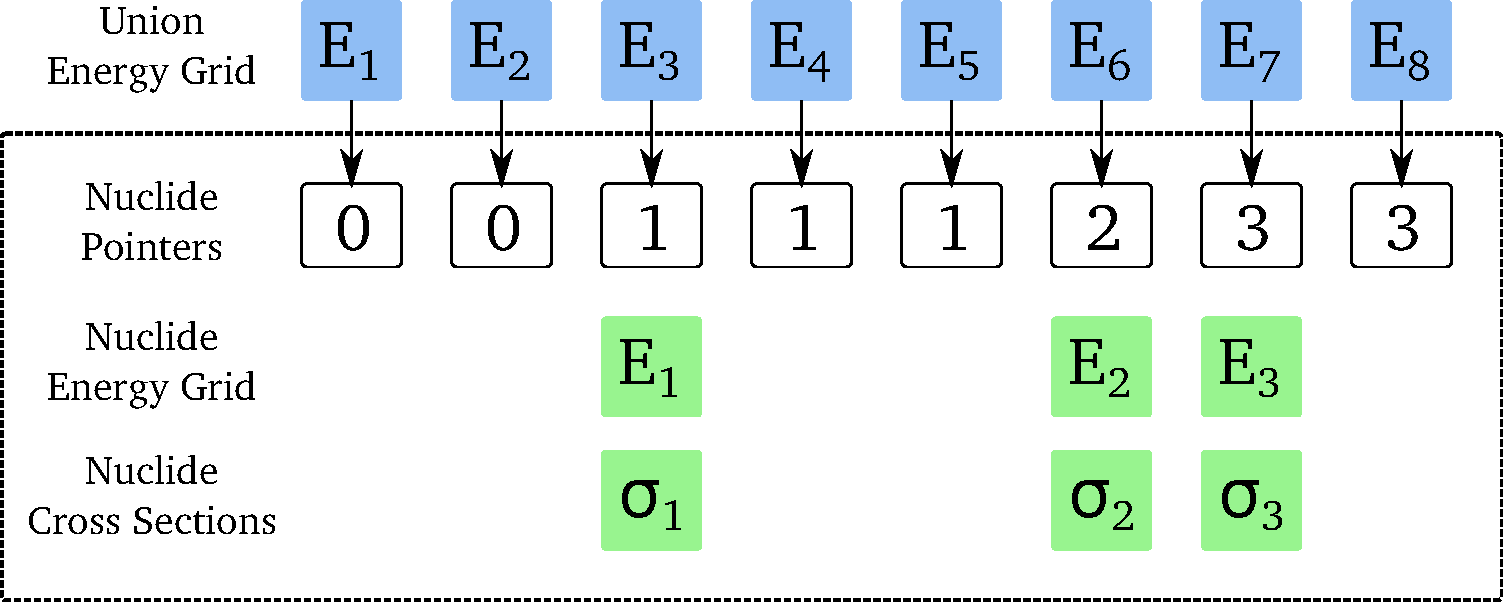
\includegraphics[width=6.0in]{figures/ch2/uniongrid.pdf}
  \caption{Mapping of union energy grid to nuclide energy grid through
    pointers.}
  \label{fig:uniongrid}
\end{figure}

\section{Random Number Generation}

In order to sample probability distributions, one must be able to produce random
numbers. The standard technique to do this is to generate numbers on the
interval $[0,1)$ from a deterministic sequence that has properties that make it
  appear to be random, e.g. being uniformly distributed and not exhibiting
  correlation between successive terms. Since the numbers produced this way are
  not truly ``random'' in a strict sense, they are typically referred to as
  pseudorandom numbers, and the techniques used to generate them are
  pseudorandom number generators (PRNGs). Numbers sampled on the unit interval
  can then be transformed for the purpose of sampling other continuous or
  discrete probability distributions.

There are a great number of algorithms for generating random numbers. One of the
simplest and commonly used algorithms is called a linear congruential generator
(LCG). We start with a random number \emph{seed} $\xi_0$ and a sequence of
random numbers can then be generated using the following recurrence relation:
\begin{equation}
  \label{eq:lcg}
  \xi_{i+1} = g \xi_i + c \mod M
\end{equation}
where $g$, $c$, and $M$ are constants. The choice of these constants will have a
profound effect on the quality and performance of the generator, so they should
not be chosen arbitrarily. As Donald Knuth stated in his seminal work \emph{The
  Art of Computer Programming} \cite{knuth-2006}, ``random numbers should not be
generated with a method chosen at random. Some theory should be used.''
Typically, $M$ is chosen to be a power of two as this enables $x \mod M$ to be
performed using the bitwise AND operator with a bit mask. The constants for the
linear congruential generator used by default in OpenMC are $g =
2806196910506780709$, $c = 1$, and $M = 2^{63}$ \cite{mathcomp-lecuyer-1999}.

One of the important capabilities for a random number generator is to be able to
skip ahead in the sequence of random numbers. Without this capability, it would
be very difficult to maintain reproducibility in a parallel calculation. If we
want to skip ahead $N$ random numbers and $N$ is large, the cost of sampling $N$
random numbers to get to that position may be prohibitively
expensive. Fortunately, algorithms have been developed that allow us to skip
ahead in $O(\log N)$ operations instead of $O(N)$. One algorithm to do so is
described in a paper by Brown \cite{trans-brown-1994}. This algorithm relies on
the following relationship:
\begin{equation}
  \label{eq:lcg-skipahead}
  \xi_{i+k} = g^k \xi_i + c \frac{g^k - 1}{g - 1} \mod M
\end{equation}
Note that \eqref{eq:lcg-skipahead} has the same general form as \eqref{eq:lcg},
so the idea is to determine the new multiplicative and additive constants in
$O(\log N)$ operations.

\section{Physics}

\subsection{Sampling Distance to Next Collision}

As a particle travels through a homogeneous material, the probability
distribution function for the distance to its next collision $\ell$ is
\begin{equation}
  \label{eq:distance-pdf}
  p(\ell) d\ell = \Sigma_t e^{-\Sigma_t \ell} d\ell
\end{equation}
where $\Sigma_t$ is the total macroscopic cross section of the
material. Equation \eqref{eq:distance-pdf} tells us that the further the
distance is to the next collision, the less likely the particle will travel that
distance. In order to sample the probability distribution function, we first
need to convert it to a cumulative distribution function
\begin{equation}
  \label{eq:distance-cdf}
  \int_0^{\ell} d\ell' p(\ell') = \int_0^{\ell} d\ell' \Sigma_t e^{-\Sigma_t
    \ell'} = 1 - e^{-\Sigma_t \ell}.
\end{equation}
By setting the cumulative distribution function equal to $\xi$, a random number
on the unit interval, and solving for the distance $\ell$, we obtain a formula
for sampling the distance to next collision:
\begin{equation}
  \label{eq:sample-distance-1}
  \ell = -\frac{\ln (1 - \xi)}{\Sigma_t}
\end{equation}
Since $\xi$ is uniformly distributed on $[0,1)$, this implies that $1 - \xi$ is
  also uniformly distributed on $[0,1)$ as well. Thus, the formula used to
    calculate the distance to next collision in OpenMC is
\begin{equation}
  \label{eq:sample-distance-2}
  \ell = -\frac{\ln \xi}{\Sigma_t}.
\end{equation}

\subsection{\texorpdfstring{$(n,\gamma)$}{(n,gamma)} and Other Disappearance Reactions}

All absorption reactions other than fission do not produce any secondary
neutrons. As a result, these are the easiest type of reactions to handle. When a
collision occurs, the first step is to sample a nuclide within a material. Once
the nuclide has been sampled, then a specific reaction for that nuclide is
sampled. Since the total absorption cross section is pre-calculated at the
beginning of a simulation, the first step in sampling a reaction is to determine
whether a ``disappearance'' reaction occurs where no secondary neutrons are
produced. This is done by sampling a random number $\xi$ on the interval $[0,1)$
  and checking whether
\begin{equation}
  \label{eq:disappearance}
  \xi \sigma_t (E) < \sigma_a (E) - \sigma_f (E)
\end{equation}
where $\sigma_t$ is the total cross section, $\sigma_a$ is the absorption cross
section (this includes fission), and $\sigma_f$ is the total fission cross
section. If this condition is met, then the neutron is killed and we proceed to
simulate the next neutron from the source bank.

No secondary particles from disappearance reactions such as photons or
alpha-particles are produced or tracked in OpenMC. To truly capture the affects
of gamma heating, it would be necessary to explicitly track photons originating
from $(n,\gamma)$ and other reactions.

\subsection{Elastic Scattering}

Elastic scattering refers to the process by which a neutron scatters off a
nucleus and does not leave it in an excited. It is referred to as ``elastic''
because in the center-of-mass system, the neutron does not actually lose
energy. However, in lab coordinates, the neutron does indeed lose
energy. Elastic scattering can be treated exactly in a Monte Carlo code thanks
to its simplicity.

Let us discuss how OpenMC handles two-body elastic scattering kinematics. The
first step is to determine whether the target nucleus has any associated
motion. Above a certain energy threshold (400 kT by default), all scattering is
assumed to take place with the target at rest. Below this threshold though, we
must account for the thermal motion of the target nucleus. Methods to sample the
velocity of the target nucleus are described later in section
\autoref{sec:freegas}. For the time being, let us assume that we have sampled
the target velocity $\mathbf{v}_t$. The velocity of the center-of-mass system is
calculated as
\begin{equation}
  \label{eq:velocity-com}
  \mathbf{v}_{cm} = \frac{\mathbf{v}_n + A \mathbf{v}_t}{A + 1}
\end{equation}
where $\mathbf{v}_n$ is the velocity of the neutron and $A$ is the atomic mass
of the target nucleus measured in neutron masses (commonly referred to as the
\emph{atomic weight ratio}). With the velocity of the center-of-mass calculated,
we can then determine the neutron's velocity in the center-of-mass system:
\begin{equation}
  \label{eq:velocity-neutron-com}
  \mathbf{V}_n = \mathbf{v}_n - \mathbf{v}_{cm}
\end{equation}
where we have used uppercase $\mathbf{V}$ to denote the center-of-mass
system. The direction of the neutron in the center-of-mass system is
\begin{equation}
  \label{eq:angle-neutron-com}
  \mathbf{\Omega}_n = \frac{\mathbf{V}_n}{|| \mathbf{V}_n ||}.
\end{equation}
At low energies, elastic scattering will be isotropic in the center-of-mass
system, but for higher energies, there may be p-wave and higher order scattering
that leads to anisotropic scattering. Thus, in general, we need to sample a
cosine of the scattering angle which we will refer to as $\mu$. For elastic
scattering, the secondary angle distribution is always given in the
center-of-mass system and is sampled according to the procedure outlined in
\autoref{sec:sample-angle}. After the cosine of the angle of scattering has been
sampled, we need to determine the neutron's new direction $\mathbf{\Omega}'_n$
in the center-of-mass system. This is done with the procedure in
\autoref{sec:transform-coordinates}. The new direction is multiplied by the
speed of the neutron in the center-of-mass system to obtain the new velocity
vector in the center-of-mass:
\begin{equation}
  \label{eq:velocity-neutron-com-2}
  \mathbf{V}'_n = || \mathbf{V}_n || \mathbf{\Omega}'_n.
\end{equation}
Finally, we transform the velocity in the center-of-mass system back to lab
coordinates:
\begin{equation}
  \label{eq:velocity-neutron-lab}
  \mathbf{v}'_n = \mathbf{V}'_n + \mathbf{v}_{cm}.
\end{equation}
In OpenMC, the angle and energy of the neutron are stored rather than the
velocity vector itself, so the post-collision angle and energy can be inferred
from the post-collision velocity of the neutron in the lab system.

For tallies that require the scattering cosine, it is important to store the
scattering cosine in the lab system. If we know the scattering cosine in the
center-of-mass, the scattering cosine in the lab system can be calculated as
\begin{equation}
  \label{eq:cosine-lab}
  \mu_{lab} = \frac{1 + A\mu}{\sqrt{A^2 + 2A\mu + 1}}.
\end{equation}
However, \eqref{eq:cosine-lab} is only valid if the target was at rest. When the
target nucleus does have thermal motion, the cosine of the scattering angle can
be determined by simply taking the dot product of the neutron's initial and
final direction in the lab system.

\subsection{Inelastic Scattering}
\label{sec:inelastic-scatter}

The major algorithms for inelastic scattering were described in previous
sections. First, a scattering cosine is sampled using the algorithms in
\autoref{sec:sample-angle}. Then an outgoing energy is sampled using the
algorithms in \autoref{sec:sample-energy}. If the outgoing energy and scattering
cosine were given in the center-of-mass system, they are transformed to
laboratory coordinates using the algorithm described in
\autoref{sec:transform-coordinates}. Finally, the direction of the particle is
changed also using the procedure in \autoref{sec:transform-coordinates}.

Although inelastic scattering leaves the target nucleus in an excited state, no
secondary photons from nuclear de-excitation are tracked in OpenMC.

\subsection{$(n,xn)$ Reactions}

These types of reactions are just treated as inelastic scattering and as such
are subject to the same procedure as described in
\autoref{sec:inelastic-scatter}. Rather than tracking multiple secondary
neutrons, the weight of the outgoing neutron is multiplied by the number of
secondary neutrons, e.g. for $(n,2n)$, only one outgoing neutron is tracked but
its weight is doubled.

\subsection{Fission}
\label{sec:fission}

While fission is normally considered an absorption reaction, from the
perspective of a Monte Carlo simulation it actually bears more similarities to
inelastic scattering since fission results in secondary neutrons in the exit
channel. Other absorption reactions like $(n,\gamma)$ or $(n,\alpha)$, on the
contrary, produce no neutrons. There are a few other idiosyncrasies in treating
fission. In a criticality calculation, secondary neutrons from fission are only
``banked'' for use in the next generation rather than being tracked as secondary
neutrons from elastic and inelastic scattering would be. On top of this, fission
is sometimes broken into first-chance fission, second-chance fission, etc. An
ACE table either lists the partial fission reactions with secondary energy
distributions for each one, or a total fission reaction with a single secondary
energy distribution.

When a fission reaction is sampled in OpenMC (either total fission or, if data
exists, first- or second-chance fission), the following algorithm is used to
create and store fission sites for the following generation. First, the average
number of prompt and delayed neutrons must be determined to decide whether the
secondary neutrons will be prompt or delayed. This is important because delayed
neutrons have a markedly different spectrum from prompt neutrons, one that has a
lower average energy of emission. The total number of neutrons emitted $\nu_t$
is given as a function of incident energy in the ACE format. Two representations
exist for $\nu_t$. The first is a polynomial of order $N$ with coefficients
$c_0,c_1,\dots,c_N$. If $\nu_t$ has this format, we can evaluate it at incoming
energy $E$ by using the equation
\begin{equation}
  \label{eq:nu-polynomial}
  \nu_t (E) = \sum_{i = 0}^N c_i E^i.
\end{equation}
The other representation is just a tabulated function with a specified
interpolation law. The number of prompt neutrons released per fission event
$\nu_p$ is also given as a function of incident energy and can be specified in a
polynomial or tabular format. The number of delayed neutrons released per
fission event $\nu_d$ can only be specified in a tabular format. In practice, we
only need to determine $nu_t$ and $nu_d$. Once these have been determined, we
can calculate the delayed neutron fraction
\begin{equation}
  \label{eq:beta}
  \beta = \frac{\nu_d}{\nu_t}.
\end{equation}
We then need to determine how many total neutrons should be emitted from
fission. If survival biasing is not being used, then the number of neutrons
emitted is
\begin{equation}
  \label{eq:fission-neutrons}
  \nu = \frac{w \nu_t}{k_{eff}}
\end{equation}
where $w$ is the statistical weight and $k_{eff}$ is the effective
multiplication factor from the previous generation. The number of neutrons
produced is biased in this manner so that the expected number of fission
neutrons produced is the number of source particles that we started with in the
generation. Since $\nu$ is not an integer, we use the following procedure to
obtain an integral number of fission neutrons to produce. If $\xi > \nu -
\lfloor \nu \rfloor$, then we produce $\lfloor \nu \rfloor$ neutrons. Otherwise,
we produce $\lfloor \nu \rfloor + 1$ neutrons. Then, for each fission site
produced, we sample the outgoing angle and energy according to the algorithms
given in \autoref{sec:sample-angle} and \autoref{sec:sample-energy}
respectively. If the neutron is to be born delayed, then there is an extra step
of sampling a delayed neutron precursor group since they each have an associated
secondary energy distribution.

The sampled outgoing angle and energy of fission neutrons along with the
position of the collision site are stored in an array called the fission
bank. In a subsequent generation, these fission bank sites are used as starting
source sites.

\subsection{Sampling Secondary Angle Distributions}
\label{sec:sample-angle}

For any reactions with secondary neutrons, it is necessary to sample secondary
angle and energy distributions. This includes elastic and inelastic scattering,
fission, and $(n,xn)$ reactions. In some cases, the angle and energy
distributions may be specified separately, and in other cases, they may be
specified as a correlated angle-energy distribution. In the following sections,
we will outline the methods used to sample secondary distributions as well as
how they are used to modify the state of a particle.

For elastic scattering, it is only necessary to specific a secondary angle
distribution since the outgoing energy can be determined analytically. Other
reactions may also have separate secondary angle and secondary energy
distributions that are uncorrelated. In these cases, the secondary angle
distribution is represented as either
\begin{itemize}
\item An Isotropic angular distribution,
\item An equiprobable distribution with 32 bins, or
\item A tabular distribution.
\end{itemize}

\subsubsection{Isotropic Angular Distribution}

In the first case, no data needs to be stored on the ACE table, and the cosine
of the scattering angle is simply calculated as
\begin{equation}
  \label{eq:isotropic-angle}
  \mu = 2\xi - 1
\end{equation}
where $\mu$ is the cosine of the scattering angle and $\xi$ is a random number
sampled uniformly on $[0,1)$.

\subsubsection{Equiprobable Angle Bin Distribution}

For a 32 equiprobable bin distribution, we select a random number $\xi$ to
sample a cosine bin $i$ such that
\begin{equation}
  \label{eq:equiprobable-bin}
  i = 1 + \lfloor 32\xi \rfloor.
\end{equation}
The same random number can then also be used to interpolate between neighboring
$\mu$ values to get the final scattering cosine:
\begin{equation}
  \label{eq:equiprobable-cosine}
  \mu = \mu_i + (32\xi - i) (\mu_{i+1} - \mu_i)
\end{equation}
where $\mu_i$ is the $i$th scattering cosine.

\subsubsection{Tabular Angular Distribution}
\label{sec:angle-tabular}

As the MCNP Manual points out \cite{lanl-x5-2008}, using an equiprobable bin
distribution works well for high-probability regions of the scattering cosine,
but for low-probability regions it is not very accurate. Thus, a more accurate
method is to represent the scattering cosine with a tabular distribution. In
this case, we have a table of cosines and their corresponding values for a
probability distribution function and cumulative distribution function. For each
incoming neutron energy $E_i$, let us call $p_{i,j}$ the $j$th value in the
probability distribution function and $c_{i,j}$ the $j$th value in the
cumulative distribution function. We first find the interpolation factor on the
incoming energy grid:
\begin{equation}
  \label{eq:interpolation-factor}
  f = \frac{E - E_i}{E_{i+1} - E_i}
\end{equation}
where $E$ is the incoming energy of the particle. Then, statistical
interpolation is performed to choose between using the cosines and distribution
functions corresponding to energy $E_i$ and $E_{i+1}$. Let $\ell$ be the chosen
table where $\ell = i$ if $\xi_1 > f$ and $\ell = i + 1$ otherwise, and $\xi_1$
is a random number. Another random number $\xi_2$ is used to sample a scattering
cosine bin $j$ using the cumulative distribution function:
\begin{equation}
  \label{eq:sample-cdf}
  c_{\ell,j} < \xi_2 < c_{\ell,j+1}.
\end{equation}
The final scattering cosine will depend on whether histogram or linear-linear
interpolation is used. In general, we can write the cumulative distribution
function as
\begin{equation}
  \label{eq:cdf}
  c(\mu) = \int_{-1}^\mu p(\mu') d\mu'
\end{equation}
where $c(\mu)$ is the cumulative distribution function and $p(\mu)$
is the probability distribution function. Since we know that
$c(\mu_{\ell,j}) = c_{\ell,j}$, this implies that for $\mu >
\mu_{\ell,j}$,
\begin{equation}
  \label{eq:cdf-2}
  c(\mu) = c_{\ell,j} + \int_{\mu_{\ell,j}}^{\mu} p(\mu') d\mu'
\end{equation}

For histogram interpolation, we have that $p(\mu') = p_{\ell,j}$ for
$\mu_{\ell,j} \le \mu' < \mu_{\ell,j+1}$. Thus, after integrating
\eqref{eq:cdf-2} we have that
\begin{equation}
  \label{eq:cumulative-dist-histogram}
  c(\mu) = c_{\ell,j} + (\mu - \mu_{\ell,j}) p_{\ell,j} = \xi_2.
\end{equation}
Solving for the scattering cosine, we obtain the final form for histogram
interpolation:
\begin{equation}
  \label{eq:cosine-histogram}
  \mu = \mu_{\ell,j} + \frac{\xi_2 - c_{\ell,j}}{p_{\ell,j}}.
\end{equation}

For linear-linear interpolation, we represent the function $p(\mu')$ as a
first-order polynomial in $\mu'$. If we interpolate between successive values on
the probability distribution function, we have that
\begin{equation}
  \label{eq:pdf-interpolation}
    p(\mu') - p_{\ell,j} = \frac{p_{\ell,j+1} - p_{\ell,j}}{\mu_{\ell,j+1} -
    \mu_{\ell,j}} (\mu' - \mu_{\ell,j}).
\end{equation}
Solving for $p(\mu')$ in \eqref{eq:pdf-interpolation} and inserting it into
\eqref{eq:cdf-2}, we obtain
\begin{equation}
  \label{eq:cdf-linlin}
    c(\mu) = c_{\ell,j} + \int_{\mu_{\ell,j}}^{\mu} \left [ \frac{p_{\ell,j+1} -
    p_{\ell,j}}{\mu_{\ell,j+1} - \mu_{\ell,j}} (\mu' - \mu_{\ell,j}) +
    p_{\ell,j} \right ] d\mu'.
\end{equation}
Let us now make a change of variables using
\begin{equation}
  \label{eq:introduce-eta}
    \eta = \frac{p_{\ell,j+1} - p_{\ell,j}}{\mu_{\ell,j+1} - \mu_{\ell,j}}
    (\mu' - \mu_{\ell,j}) + p_{\ell,j}.
\end{equation}
Equation \eqref{eq:cdf-linlin} then becomes
\begin{equation}
  \label{eq:cdf-linlin-eta}
    c(\mu) = c_{\ell,j} + \frac{1}{m} \int_{p_{\ell,j}}^{m(\mu - \mu_{\ell,j}) +
    p_{\ell,j}} \eta \, d\eta
\end{equation}
where we have used
\begin{equation}
  \label{eq:slope}
    m = \frac{p_{\ell,j+1} - p_{\ell,j}}{\mu_{\ell,j+1} - \mu_{\ell,j}}.
\end{equation}
Integrating \eqref{eq:cdf-linlin-eta}, we have
\begin{equation}
  \label{eq:cdf-linlin-integrated}
    c(\mu) = c_{\ell,j} + \frac{1}{2m} \left ( \left [ m (\mu - \mu_{\ell,j} ) +
    p_{\ell,j} \right ]^2 - p_{\ell,j}^2 \right ) = \xi_2.
\end{equation}
Solving for $\mu$, we have the final form for the scattering cosine using a
tabular distribution and linear-linear interpolation:
\begin{equation}
  \label{eq:cosine-linlin}
    \mu = \mu_{\ell,j} + \frac{1}{m} \left ( \sqrt{p_{\ell,j}^2 + 2 m (\xi_2 -
    c_{\ell,j} )} - p_{\ell,j} \right ).
\end{equation}

\subsection{Sampling Secondary Energy and Correlated Angle/Energy Distributions}
\label{sec:sample-energy}

For a reaction with secondary neutrons, it is necessary to determine the
outgoing energy of the neutrons. For any reaction other than elastic scattering,
the outgoing energy must be determined based on tabulated or parameterized
data. The ENDF-6 Format \cite{bnl-herman-2009} specifies a variety of ways that
the secondary energy distribution can be represented. ENDF File 5 contains
uncorrelated energy distribution whereas ENDF File 6 contains correlated
energy-angle distributions. The ACE format specifies its own representations
based loosely on the formats given in ENDF-6. In this section, we will describe
how the outgoing energy of secondary particles is determined based on each ACE
law.

One of the subtleties in the ACE format is the fact that a single reaction can
have multiple secondary energy distributions. This is mainly useful for
reactions with multiple neutrons in the exit channel such as $(n,2n)$ or
$(n,3n)$. In these types of reactions, each neutron is emitted corresponding to
a different excitation level of the compound nucleus, and thus in general the
neutrons will originate from different energy distributions. The first step in
sampling a secondary energy is to sample between multiple energy distributions
if more than one is present.

Once a secondary energy distribution has been sampled, the procedure for
determining the outgoing energy will depend on which ACE law has been specified
for the data.

\subsubsection{ACE Law 1 - Tabular Equiprobable Energy Bins}
\label{sec:ace-law-1}

In the tabular equiprobable bin representation, an array of equiprobable
outgoing energy bins is given for a number of incident energies. While the
representation itself is simple, the complexity lies in how one interpolates
between incident as well as outgoing energies on such a table. If one performs
simple interpolation between tables for neighboring incident energies, it is
possible that the resulting energies would violate laws governing the
kinematics, i.e. the outgoing energy may be outside the range of available
energy in the reaction.

To avoid this situation, the accepted practice is to use a process known as
scaled interpolation \cite{nse-doyas-1972}. First, we find the tabulated
incident energies which bound the actual incoming energy of the particle,
i.e. find $i$ such that $E_i < E < E_{i+1}$ and calculate the interpolation
factor $f$ via \eqref{eq:interpolation-factor}. Then, we interpolate between the
minimum and maximum energies of the outgoing energy distributions corresponding
to $E_i$ and $E_{i+1}$:
\begin{equation}
  \label{eq:ace-law-1-minmax}
  \begin{split}
    E_{min} &= E_{i,1} + f ( E_{i+1,1} - E_i ) \\
    E_{max} &= E_{i,M} + f ( E_{i+1,M} - E_M )
  \end{split}
\end{equation}
where $E_{min}$ and $E_{max}$ are the minimum and maximum outgoing energies of a
scaled distribution, $E_{i,j}$ is the $j$th outgoing energy corresponding to the
incoming energy $E_i$, and $M$ is the number of outgoing energy bins. Next,
statistical interpolation is performed to choose between using the outgoing
energy distributions corresponding to energy $E_i$ and $E_{i+1}$. Let $\ell$ be
the chosen table where $\ell = i$ if $\xi_1 > f$ and $\ell = i + 1$ otherwise,
and $\xi_1$ is a random number. Now, we randomly sample an equiprobable outgoing
energy bin $j$ and interpolate between successive values on the outgoing energy
distribution:
\begin{equation}
  \label{eq:ace-law-1-intermediate}
  \hat{E} = E_{\ell,j} + \xi_2 (E_{\ell,j+1} - E_{\ell,j})
\end{equation}
where $\xi_2$ is a random number sampled uniformly on $[0,1)$. Since
this outgoing energy may violate reaction kinematics, we then scale it to the
minimum and maximum energies we calculated earlier to get the final outgoing
energy:
\begin{equation}
  \label{eq:ace-law-1-energy}
  E' = E_{min} + \frac{\hat{E} - E_{\ell,1}}{E_{\ell,M} - E_{\ell,1}}
  (E_{max} - E_{min}).
\end{equation}

\subsubsection{ACE Law 3 - Inelastic Level Scattering}

It can be shown \cite{foderaro-1971} that in inelastic level scattering, the
outgoing energy of the neutron $E'$ can be related to the Q-value of the
reaction and the incoming energy:
\begin{equation}
  \label{eq:level-scattering}
  E' = \left ( \frac{A}{A+1} \right )^2 \left ( E - \frac{A + 1}{A} Q \right )
\end{equation}
where $A$ is the mass of the target nucleus measured in neutron masses.

\subsubsection{ACE Law 4 - Continuous Tabular Distribution}
\label{sec:ace-law-4}

This representation is very similar that in \autoref{sec:ace-law-1} except that
instead of equiprobable outgoing energy bins, the outgoing energy distribution
for each incoming energy is represented with a probability distribution
function. For each incoming neutron energy $E_i$, let us call $p_{i,j}$ the
$j$th value in the probability distribution function, $c_{i,j}$ the $j$th value
in the cumulative distribution function, and $E_{i,j}$ the $j$th outgoing
energy.

We proceed first as we did for ACE Law 1, determining the bounding energies of
the particle's incoming energy such that $E_i < E < E_{i+1}$ and calculating an
interpolation factor $f$ with \eqref{eq:interpolation-factor}. Next, statistical
interpolation is performed to choose between using the outgoing energy
distributions corresponding to energy $E_i$ and $E_{i+1}$. Let $\ell$ be the
chosen table where $\ell = i$ if $\xi_1 > f$ and $\ell = i + 1$ otherwise, and
$\xi_1$ is a random number. Then, we sample an outgoing energy bin $j$ using the
cumulative distribution function:
\begin{equation}
  \label{eq:ace-law-4-sample-cdf}
  c_{\ell,j} < \xi_2 < c_{\ell,j+1}
\end{equation}
where $\xi_2$ is a random number sampled uniformly on $[0,1)$. At this point, we
  need to interpolate between the successive values on the outgoing energy
  distribution using either histogram or linear-linear interpolation. The
  formulas for these can be derived along the same lines as those found in
  \autoref{sec:angle-tabular}. For histogram interpolation, the interpolated
  outgoing energy on the $\ell$th distribution is
\begin{equation}
  \label{eq:energy-histogram}
  \hat{E} = E_{\ell,j} + \frac{\xi_2 - c_{\ell,j}}{p_{\ell,j}}
\end{equation}
If linear-linear interpolation is to be used, the outgoing energy on the
$\ell$th distribution is
\begin{equation}
  \label{eq:energy-linlin}
  \hat{E} = E_{\ell,j} + \frac{E_{\ell,j+1} - E_{\ell,j}}{p_{\ell,j+1} -
    p_{\ell,j}} \left ( \sqrt{p_{\ell,j}^2 + 2 \frac{p_{\ell,j+1} -
      p_{\ell,j}}{E_{\ell,j+1} - E_{\ell,j}} ( \xi_2 - c_{\ell,j} )} -
  p_{\ell,j} \right )
\end{equation}
Since this outgoing energy may violate reaction kinematics, we then scale it to
minimum and maximum energies interpolated between the neighboring outgoing
energy distributions to get the final outgoing energy:
\begin{equation}
  \label{eq:ace-law-4-energy}
  E' = E_{min} + \frac{\hat{E} - E_{\ell,1}}{E_{\ell,M} - E_{\ell,1}}
  (E_{max} - E_{min})
\end{equation}
where $E_{min}$ and $E_{max}$ are defined the same as in
\eqref{eq:ace-law-1-minmax}.

\subsubsection{ACE Law 7 - Maxwell Fission Spectrum}
\label{sec:maxwell}

One representation of the secondary energies for neutrons from fission is the
so-called Maxwell spectrum. A probability distribution for the Maxwell spectrum
can be written in the form
\begin{equation}
  \label{eq:maxwell-spectrum}
  p(E') dE' = c E'^{1/2} e^{-E'/T(E)} dE'
\end{equation}
where $E$ is the incoming energy of the neutron and $T$ is the so-called nuclear
temperature, which is a function of the incoming energy of the neutron. The ACE
format contains a list of nuclear temperatures versus incoming energies. The
nuclear temperature is interpolated between neighboring incoming energies using
a specified interpolation law. Once the temperature $T$ is determined, we then
calculate a candidate outgoing energy based on rule C64 in the Monte Carlo
Sampler \cite{lanl-everett-1983}:
\begin{equation}
  \label{eq:maxwell-E-candidate}
  E' = -T \left [ \log (\xi_1) + \log (\xi_2) \cos^2 \left ( \frac{\pi
      \xi_3}{2} \right ) \right ]
\end{equation}
where $\xi_1, \xi_2, \xi_3$ are random numbers sampled on the unit
interval. The outgoing energy is only accepted if
\begin{equation}
  \label{eq:maxwell-restriction}
  0 \le E' \le E - U
\end{equation}
where $U$ is called the restriction energy and is specified on the ACE table. If
the outgoing energy is rejected, it is resampled using
\eqref{eq:maxwell-E-candidate}.

\subsubsection{ACE Law 9 - Evaporation Spectrum}

Evaporation spectra are primarily used in compound nucleus processes where a
secondary particle can ``evaporate'' from the compound nucleus if it has
sufficient energy. The probability distribution for an evaporation spectrum can
be written in the form
\begin{equation}
  \label{eq:evaporation-spectrum}
  p(E') dE' = c E' e^{-E'/T(E)} dE'
\end{equation}
where $E$ is the incoming energy of the neutron and $T$ is the nuclear
temperature, which is a function of the incoming energy of the neutron. The ACE
format contains a list of nuclear temperatures versus incoming energies. The
nuclear temperature is interpolated between neighboring incoming energies using
a specified interpolation law. Once the temperature $T$ is determined, we then
calculate a candidate outgoing energy based on rule C45 in the Monte Carlo
Sampler \cite{lanl-everett-1983}:
\begin{equation}
  \label{eq:evaporation-E}
  E' = -T \log (\xi_1 \xi_2)
\end{equation}
where $\xi_1, \xi_2$ are random numbers sampled on the unit interval. The
outgoing energy is only accepted according to a specified restriction energy as
in \eqref{eq:maxwell-restriction}.

\subsubsection{ACE Law 11 - Energy-Dependent Watt Spectrum}

The probability distribution for a Watt fission spectrum
\cite{physrev-watt-1952} can be written in the form
\begin{equation}
  \label{eq:watt-spectrum}
  p(E') dE' = c e^{-E'/a(E)} \sinh \sqrt{b(E) \, E'} dE'
\end{equation}
where $a$ and $b$ are parameters for the distribution and are given as tabulated
functions of the incoming energy of the neutron. These two parameters are
interpolated on the incoming energy grid using a specified interpolation
law. Once the parameters have been determined, we sample a Maxwellian spectrum
with nuclear temperature $a$ using the algorithm described in
\autoref{sec:maxwell} to get an energy $W$. Then, the outgoing energy is
calculated as
\begin{equation}
  \label{eq:watt-E}
  E' = W + \frac{a^2 b}{4} + (2\xi - 1) \sqrt{a^2 b W}
\end{equation}
where $\xi$ is a random number sampled on the interval $[0,1)$. The outgoing
  energy is only accepted according to a specified restriction energy $U$ as
  defined in \eqref{eq:maxwell-restriction}.

This algorithm can be found in Forrest Brown's lectures on Monte Carlo methods
\cite{lanl-brown-2005} and is an unpublished sampling scheme based on the
original Watt spectrum derivation.

\subsubsection{ACE Law 44 - Kalbach-Mann Correlated Scattering}

This law is very similar to ACE Law 4 except now the outgoing angle of the
neutron is correlated to the outgoing energy and is not sampled from a separate
distribution. For each incident neutron energy $E_i$ tabulated, there is
an array of precompound factors $R_{i,j}$ and angular distribution slopes
$A_{i,j}$ corresponding to each outgoing energy bin $j$ in addition
to the outgoing energies and distribution functions as in ACE Law 4.

The calculation of the outgoing energy of the neutron proceeds exactly the same
as in the algorithm described in \autoref{sec:ace-law-4}. In that algorithm, we
found an interpolation factor $f$, statistically sampled an incoming energy bin
$\ell$, and sampled an outgoing energy bin $j$ based on the tabulated cumulative
distribution function. Once the outgoing energy has been determined with
\eqref{eq:ace-law-4-energy}, we then need to calculate the outgoing angle based
on the tabulated Kalbach-Mann parameters. These parameters themselves are
subject to either histogram or linear-linear interpolation on the outgoing
energy grid. For histogram interpolation, the parameters are
\begin{equation}
  \label{eq:KM-parameters-histogram}
  \begin{split}
    R &= R_{\ell,j} \\ 
    A &= A_{\ell,j}
  \end{split}
\end{equation}
If linear-linear interpolation is specified, the parameters are
\begin{equation}
  \label{eq:KM-parameters-linlin}
  \begin{split}
    R &= R_{\ell,j} + \frac{\hat{E} - E_{\ell,j}}{E_{\ell,j+1} - E_{\ell,j}} (
    R_{\ell,j+1} - R_{\ell,j} ) \\
    A &= A_{\ell,j} + \frac{\hat{E} - E_{\ell,j}}{E_{\ell,j+1} - E_{\ell,j}} (
    A_{\ell,j+1} - A_{\ell,j} )
  \end{split}
\end{equation}
where $\hat{E}$ is defined in \eqref{eq:energy-linlin}. With the parameters
determined, the probability distribution function for the cosine of the
scattering angle is
\begin{equation}
  \label{eq:KM-pdf-angle}
  p(\mu) d\mu = \frac{A}{2 \sinh (A)} \left [ \cosh (A\mu) + R \sinh (A\mu)
    \right ] d\mu
\end{equation}
The rules for sampling this probability distribution function can be derived
based on rules C39 and C40 in the Monte Carlo Sampler
\cite{lanl-everett-1983}. First, we sample two random numbers $\xi_3, \xi_4$ on
the unit interval. If $\xi_3 > R$ then the outgoing angle is
\begin{equation}
  \label{eq:KM-angle-1}
  \mu = \frac{1}{A} \ln \left ( T + \sqrt{T^2 + 1} \right )
\end{equation}
where $T = (2 \xi_4 - 1) \sinh (A)$. If $\xi_3 \le R$, then the
outgoing angle is
\begin{equation}
  \label{eq:KM-angle-2}
  \mu = \frac{1}{A} \ln \left ( \xi_4 e^A + (1 - \xi_4) e^{-A} \right )
\end{equation}

\subsubsection{ACE Law 61 - Correlated Energy and Angle Distribution}

This law is very similar to ACE Law 44 in the sense that the outgoing angle of
the neutron is correlated to the outgoing energy and is not sampled from a
separate distribution. In this case though, rather than being determined from an
analytical distribution function, the cosine of the scattering angle is
determined from a tabulated distribution. For each incident energy $i$ and
outgoing energy $j$, there is a tabulated angular distribution.

The calculation of the outgoing energy of the neutron proceeds exactly the same
as in the algorithm described in \autoref{sec:ace-law-4}. In that algorithm, we
found an interpolation factor $f$, statistically sampled an incoming energy bin
$\ell$, and sampled an outgoing energy bin $j$ based on the tabulated cumulative
distribution function. Once the outgoing energy has been determined with
\eqref{eq:ace-law-4-energy}, we then need to decide which angular distribution
to use. If histogram interpolation was used on the outgoing energy bins, then we
use the angular distribution corresponding to incoming energy bin $\ell$ and
outgoing energy bin $j$. If linear-linear interpolation was used on the outgoing
energy bins, then we use whichever angular distribution was closer to the
sampled value of the cumulative distribution function for the outgoing
energy. The actual algorithm used to sample the chosen tabular angular
distribution has been previously described in \autoref{sec:angle-tabular}.

\subsubsection{ACE Law 66 - N-Body Phase Space Distribution}

Reactions in which there are more than two products of similar masses are
sometimes best treated by using what's known as an N-body phase
distribution. This distribution has the following probability density function
for outgoing energy of the $i$th particle in the center-of-mass system:
\begin{equation}
  \label{eq:n-body-pdf}
  p_i(E') dE' = C_n \sqrt{E'} (E_i^{max} - E')^{(3n/2) - 4} dE'
\end{equation}
where $n$ is the number of outgoing particles, $C_n$ is a normalization
constant, $E_i^{max}$ is the maximum center-of-mass energy for particle $i$, and
$E'$ is the outgoing energy. The algorithm for sampling the outgoing energy is
based on algorithms R28, C45, and C64 in the Monte Carlo Sampler
\cite{lanl-everett-1983}. First we calculate the maximum energy in the
center-of-mass using the following equation:
\begin{equation}
  \label{eq:n-body-emax}
  E_i^{max} = \frac{A_p - 1}{A_p} \left ( \frac{A}{A+1} E + Q \right )
\end{equation}
where $A_p$ is the total mass of the outgoing particles in neutron masses, $A$
is the mass of the original target nucleus in neutron masses, and $Q$ is the
Q-value of the reaction. Next we sample a value $x$ from a Maxwell distribution
with a nuclear temperature of one using the algorithm outlined in
\autoref{sec:maxwell}. We then need to determine a value $y$ that will depend on
how many outgoing particles there are. For $n = 3$, we simply sample another
Maxwell distribution with unity nuclear temperature. For $n = 4$, we use the
equation
\begin{equation}
  \label{eq:n-body-y4}
  y = -\ln ( \xi_1 \xi_2 \xi_3 )
\end{equation}
where $\xi_i$ are random numbers sampled on the interval
$[0,1)$. For $n = 5$, we use the equation
\begin{equation}
  \label{eq:n-body-y5}
  y = -\ln ( \xi_1 \xi_2 \xi_3 \xi_4 ) - \ln ( \xi_5 ) \cos^2 \left (
  \frac{\pi}{2} \xi_6 \right )
\end{equation}
After $x$ and $y$ have been determined, the outgoing energy is then
calculated as
\begin{equation}
  \label{eq:n-body-energy}
  E' = \frac{x}{x + y} E_i^{max}
\end{equation}
There are two important notes to make regarding the N-body phase space
distribution. First, the documentation (and code) for MCNP5 has a mistake in the
algorithm for $n = 4$. That being said, there are no existing nuclear data
evaluations which use an N-body phase space distribution with $n = 4$, so the
error would not affect any calculations. In the ENDF/B-VII.0 nuclear data
evaluation, only one reaction uses an N-body phase space distribution at all,
the $(n,2n)$ reaction with $^2$H.

\subsection{Transforming a Particle's Coordinates}
\label{sec:transform-coordinates}

Once the cosine of the scattering angle $\mu$ has been sampled either from an
angle distribution or a correlated angle-energy distribution, we are still left
with the task of transforming the particle's coordinates. If the outgoing energy
and scattering cosine were given in the center-of-mass system, then we first
need to transform these into the laboratory system. The relationship between the
outgoing energy in center-of-mass and laboratory is
\begin{equation}
  \label{eq:energy-com-to-lab}
  E' = E'_{cm} + \frac{E + 2\mu_{cm} (A + 1) \sqrt{EE'_{cm}}}{(A+1)^2}
\end{equation}
where $E'_{cm}$ is the outgoing energy in the center-of-mass system,
$\mu_{cm}$ is the scattering cosine in the center-of-mass system,
$E'$ is the outgoing energy in the laboratory system, and $E$ is the
incident neutron energy. The relationship between the scattering cosine in
center-of-mass and laboratory is
\begin{equation}
  \label{eq:angle-com-to-lab}
  \mu = \mu_{cm} \sqrt{\frac{E'_{cm}}{E'}} + \frac{1}{A + 1}
  \sqrt{\frac{E}{E'}}
\end{equation}
where $\mu$ is the scattering cosine in the laboratory system. The
scattering cosine still only tells us the cosine of the angle between the
original direction of the particle and the new direction of the particle. If we
express the pre-collision direction of the particle as $\mathbf{\Omega} =
(u,v,w)$ and the post-collision direction of the particle as
$\mathbf{\Omega}' = (u',v',w')$, it is possible to relate the pre- and
post-collision components. We first need to uniformly sample an azimuthal angle
$\phi$ in $[0, 2\pi)$. After the azimuthal angle has been sampled,
the post-collision direction is calculated as
\begin{equation}
  \label{eq:post-collision-angle}
  \begin{split}
    u' &= \mu u + \frac{\sqrt{1 - \mu^2} ( uw \cos\phi - v \sin\phi )}{\sqrt{1 -
        w^2}} \\
    v' &= \mu v + \frac{\sqrt{1 - \mu^2} ( vw \cos\phi + u \sin\phi )}{\sqrt{1 -
        w^2}} \\
    w' &= \mu w - \sqrt{1 - \mu^2} \sqrt{1 - w^2} \cos\phi.
  \end{split}
\end{equation}

\subsection{Effect of Thermal Motion on Cross-Sections}
\label{sec:freegas}

When a neutron scatters off of a nucleus, it may often be assumed that the
target nucleus is at rest. However, if the material is at a temperature greater
than 0 K, it will have motion associated with the thermal vibration. Thus, the
velocity of the neutron relative to the target nucleus is in general not the
same as the velocity of the neutron entering the collision.

The effect of the thermal motion on the interaction probability can be written
as
\begin{equation}
  \label{eq:doppler-broaden}
  v_n \bar{\sigma} (v_n, T) = \int d\mathbf{v}_T v_r \sigma(v_r)
  M (\mathbf{v}_T)
\end{equation}
where $v_n$ is the magnitude of the velocity of the neutron, $\bar{\sigma}$ is
an effective cross section, $T$ is the temperature of the target material,
$\mathbf{v}_T$ is the velocity of the target nucleus, $v_r = || \mathbf{v}_n -
\mathbf{v}_T ||$ is the magnitude of the relative velocity, $\sigma$ is the
cross section at 0 K, and $M (\mathbf{v}_T)$ is the probability distribution for
the target nucleus velocity at temperature $T$ (a Maxwellian). In a Monte Carlo
code, one must account for the effect of the thermal motion on both the
integrated cross-section as well as secondary angle and energy
distributions. For integrated cross-sections, it is possible to calculate
thermally-averaged cross-sections by applying a kernel Doppler broadening
algorithm to data at 0 K (or some temperature lower than the desired
temperature). The most ubiquitous algorithm for this purpose is the SIGMA1
method \cite{nse-cullen-1976} developed by Red Cullen and subsequently refined
by others. This method is used in the NJOY \cite{nds-macfarlane-2010} and PREPRO
\cite{iaea-cullen-2012} data processing codes.

The effect of thermal motion on secondary angle and energy distributions can be
accounted for on-the-fly in a Monte Carlo simulation. We must first qualify
where it is actually used however. All threshold reactions are treated as being
independent of temperature, and therefore they are not Doppler broadened in NJOY
and no special procedure is used to adjust the secondary angle and energy
distributions. The only non-threshold reactions with secondary neutrons are
elastic scattering and fission. For fission, it is assumed that the neutrons are
emitted isotropically (this is not strictly true, but is nevertheless a good
approximation). This leaves only elastic scattering that needs a special thermal
treatment for secondary distributions.

Fortunately, it is possible to directly sample the velocity of the target
nuclide and use it in the kinematic calculations. However, this calculation is a
bit more nuanced than it might seem at first glance. One might be tempted to
simply sample a Maxwellian distribution for the velocity of the target nuclide.
Careful inspection of \eqref{eq:doppler-broaden} however tells us that target
velocities that produce relative velocities which correspond to high cross
sections will have a greater contribution to the effective reaction rate. This
is most important when the velocity of the incoming neutron is close to a
resonance. For example, if the neutron's velocity corresponds to a trough in a
resonance elastic scattering cross-section, a very small target velocity can
cause the relative velocity to correspond to the peak of the resonance, thus
making a disproportionate contribution to the reaction rate. The conclusion is
that if we are to sample a target velocity in the Monte Carlo code, it must be
done in such a way that preserves the thermally-averaged reaction rate as per
\eqref{eq:doppler-broaden}.

The method by which most Monte Carlo codes sample the target velocity for use in
elastic scattering kinematics is outlined in detail by Gelbard
\cite{anl-gelbard-1979}. The derivation here largely follows that of
Gelbard. Let us first write the reaction rate as a function of the velocity of
the target nucleus:
\begin{equation}
  \label{eq:reaction-rate}
  R(\mathbf{v}_T) = || \mathbf{v}_n - \mathbf{v}_T || \sigma ( ||
  \mathbf{v}_n - \mathbf{v}_T || ) M ( \mathbf{v}_T )
\end{equation}
where $R$ is the reaction rate. Note that this is just the right-hand side of
\eqref{eq:doppler-broaden}. Based on the discussion above, we want to construct
a probability distribution function for sampling the target velocity to preserve
the reaction rate --- this is different from the overall probability
distribution function for the target velocity, $M ( \mathbf{v}_T )$. This
probability distribution function can be found by integrating
\eqref{eq:reaction-rate} to obtain a normalization factor:
\begin{equation}
  \label{eq:target-pdf-1}
  p( \mathbf{v}_T ) d\mathbf{v}_T = \frac{R(\mathbf{v}_T) d\mathbf{v}_T}{\int
    d\mathbf{v}_T \, R(\mathbf{v}_T)}
\end{equation}
Let us call the normalization factor in the denominator of
\eqref{eq:target-pdf-1} $C$.

It is normally assumed that $\sigma (v_r)$ is constant over the range of
relative velocities of interest. This is a good assumption for almost all cases
since the elastic scattering cross section varies slowly with velocity for light
nuclei, and for heavy nuclei where large variations can occur due to resonance
scattering, the moderating effect is rather small. Nonetheless, this assumption
may cause incorrect answers in systems with $^{238}$U where the low-lying
resonances can cause a significant amount of up-scatter that would be ignored by
this assumption. Nevertheless, with this assumption, we write $\sigma (v_r) =
\sigma_s$ which simplifies \eqref{eq:target-pdf-1} to
\begin{equation}
  \label{eq:target-pdf-2}
  p( \mathbf{v}_T ) d\mathbf{v}_T = \frac{\sigma_s}{C} || \mathbf{v}_n -
  \mathbf{v}_T || M ( \mathbf{v}_T ) d\mathbf{v}_T.
\end{equation}
The Maxwellian distribution in velocity is
\begin{equation}
  \label{eq:maxwellian-velocity}
  M (\mathbf{v}_T) = \left ( \frac{m}{2\pi kT} \right )^{3/2} \exp \left (
  \frac{-m || \mathbf{v}_T ||^2}{2kT} \right )
\end{equation}
where $m$ is the mass of the target nucleus and $k$ is Boltzmann's
constant. Notice here that the term in the exponential is dependent only on the
speed of the target, not on the actual direction. Thus, we can change the
Maxwellian into a distribution for speed rather than velocity. The differential
element of velocity is
\begin{equation}
  \label{eq:differential-velocity}
  d\mathbf{v}_T = v_T^2 dv_T d\mu d\phi.
\end{equation}
Let us define the Maxwellian distribution in speed as
\begin{equation}
  \label{eq:maxwellian-speed}
  M (v_T) dv_T = \int_{-1}^1 d\mu \int_{0}^{2\pi} d\phi \, dv_T \, v_T^2
  M(\mathbf{v}_T) = \sqrt{ \frac{2}{\pi} \left ( \frac{m}{kT} \right )^3}
  v_T^2 \exp \left ( \frac{-m v_T}{2kT} \right ) dv_T.
\end{equation}
To simplify things a bit, we'll define a parameter
\begin{equation}
  \label{eq:maxwellian-beta}
  \beta = \sqrt{\frac{m}{2kT}}.
\end{equation}
Substituting \eqref{eq:maxwellian-beta} into \eqref{eq:maxwellian-speed}, we
obtain
\begin{equation}
  \label{eq:maxwellian-speed2}
  M (v_T) dv_T = \frac{4}{\sqrt{\pi}} \beta^3 v_T^2 \exp \left ( -\beta^2
  v_T^2 \right ) dv_T.
\end{equation}
Now, changing variables in \eqref{eq:target-pdf-2} by using the result from
\eqref{eq:maxwellian-speed2}, our new probability distribution function is
\begin{equation}
  \label{eq:target-pdf-3}
  p( v_T, \mu ) dv_T d\mu = \frac{4\sigma_s}{\sqrt{\pi}C'} || \mathbf{v}_n -
  \mathbf{v}_T || \beta^3 v_T^2 \exp \left ( -\beta^2 v_T^2 \right ) dv_T d\mu.
\end{equation}
Again, the Maxwellian distribution for the speed of the target nucleus has no
dependence on the angle between the neutron and target velocity vectors. Thus,
only the term $|| \mathbf{v}_n - \mathbf{v}_T ||$ imposes any constraint
on the allowed angle. Our last task is to take that term and write it in terms
of magnitudes of the velocity vectors and the angle rather than the vectors
themselves. We can establish this relation based on the law of cosines which
tells us that
\begin{equation}
  \label{eq:lawcosine}
  2 v_n v_T \mu = v_n^2 + v_T^2 - v_r^2.
\end{equation}
Thus, we can infer that
\begin{equation}
  \label{eq:change-terms}
  || \mathbf{v}_n - \mathbf{v}_T || = || \mathbf{v}_r || = v_r = \sqrt{v_n^2 +
    v_T^2 - 2v_n v_T \mu}
\end{equation}
Inserting \eqref{eq:change-terms} into \eqref{eq:target-pdf-3}, we obtain
\begin{equation}
  \label{eq:target-pdf-4}
  p( v_T, \mu ) dv_T d\mu = \frac{4\sigma_s}{\sqrt{\pi}C'} \sqrt{v_n^2 +
    v_T^2 - 2v_n v_T \mu} \beta^3 v_T^2 \exp \left ( -\beta^2 v_T^2 \right )
  dv_T d\mu
\end{equation}
This expression is still quite formidable and does not lend itself to any
natural sampling scheme. We can divide this probability distribution into two
parts as such:
\begin{align}
  \label{eq:divide-pdf-p}
  p(v_T, \mu) &= f_1(v_T, \mu) f_2(v_T) \\
  \label{eq:divide-pdf-f1}
  f_1(v_T, \mu) &= \frac{4\sigma_s}{\sqrt{\pi} C'} \frac{ \sqrt{v_n^2 + v_T^2 -
      2v_n v_T \mu}}{v_n + v_T} \\
  \label{eq:divide-pdf-f2}
  f_2(v_T) &= (v_n + v_T) \beta^3 v_T^2 \exp \left ( -\beta^2 v_T^2 \right )
\end{align}
In general, any probability distribution function of the form $p(x) =
f_1(x) f_2(x)$ with $f_1(x)$ bounded can be sampled by sampling
$x'$ from the distribution
\begin{equation}
  \label{eq:freegas-f2}
  q(x) dx = \frac{f_2(x) dx}{\int f_2(x) dx}
\end{equation}
and accepting it with probability
\begin{equation}
  \label{eq:freegas-accept}
  p_{accept} = \frac{f_1(x')}{\max f_1(x)}
\end{equation}
The reason for dividing and multiplying the terms by $v_n + v_T$ is to ensure
that the first term is bounded. In general, $|| \mathbf{v}_n - \mathbf{v}_T ||$
can take on arbitrarily large values, but if we divide it by its maximum value
$v_n + v_T$, then it ensures that the function will be bounded. We now must come
up with a sampling scheme for \eqref{eq:freegas-f2}. To determine $q(v_T)$, we
need to integrate $f_2$ in \eqref{eq:divide-pdf-f2}. Doing so we find that
\begin{equation}
  \label{eq:integrate-f2}
  \int_0^{\infty} dv_T (v_n + v_T) \beta^3 v_T^2 \exp \left ( -\beta^2 v_T^2
  \right ) = \frac{1}{4\beta} \left ( \sqrt{\pi} \beta v_n + 2 \right ).
\end{equation}
Thus, we need to sample the probability distribution function
\begin{equation}
  \label{eq:freegas-f2-2}
  q(v_T) dv_T = \left ( \frac{4\beta^2 v_n v_T^2}{\sqrt{\pi} \beta v_n + 2} +
  \frac{4\beta^4 v_T^3}{\sqrt{\pi} \beta v_n + 2} \right ) exp \left (
  -\beta^2 v_T^2 \right )
\end{equation}
Now, let us do a change of variables with the following definitions
\begin{equation}
  \label{eq:beta-to-x}
  \begin{split}
    x &= \beta v_T \\
    y &= \beta v_n.
  \end{split}
\end{equation}
Substituting \eqref{eq:beta-to-x} into \eqref{eq:freegas-f2-2} along with $dx =
\beta dv_T$ and doing some crafty rearranging of terms yields
\begin{equation}
  \label{eq:freegas-f2-3}
  q(x) dx = \left [ \left ( \frac{\sqrt{\pi} y}{\sqrt{\pi} y + 2} \right )
    \frac{4}{\sqrt{\pi}} x^2 e^{-x^2} + \left ( \frac{2}{\sqrt{\pi} y + 2}
    \right ) 2x^3 e^{-x^2} \right ] dx.
\end{equation}
It's important to make note of the following two facts. First, the terms outside
the parentheses are properly normalized probability distribution functions that
can be sampled directly. Secondly, the terms inside the parentheses are always
less than unity. Thus, the sampling scheme for $q(x)$ is as follows. We
sample a random number $\xi_1$ on the interval $[0,1)$ and if
\begin{equation}
  \label{eq:freegas-alpha}
  \xi_1 < \frac{2}{\sqrt{\pi} y + 2}
\end{equation}
then we sample the probability distribution $2x^3 e^{-x^2}$ for $x$ using rule
C49 in the Monte Carlo Sampler \cite{lanl-everett-1983} which we can then use to
determine the speed of the target nucleus $v_T$ from
\eqref{eq:beta-to-x}. Otherwise, we sample the probability distribution
$\frac{4}{\sqrt{\pi}} x^2 e^{-x^2}$ for $x$ using rule C61 in the Monte Carlo
Sampler.

With a target speed sampled, we must then decide whether to accept it based on
the probability in \eqref{eq:freegas-accept}. The cosine can be sampled
isotropically as $\mu = 2\xi_2 - 1$ where $\xi_2$ is a random number on the unit
interval. Since the maximum value of $f_1(v_T, \mu)$ is $4\sigma_s / \sqrt{\pi}
C'$, we then sample another random number $\xi_3$ and accept the sampled target
speed and cosine if
\begin{equation}
  \label{eq:freegas-accept-2}
  \xi_3 < \frac{\sqrt{v_n^2 + v_T^2 - 2 v_n v_T \mu}}{v_n + v_T}
\end{equation}
If is not accepted, then we repeat the process and resample a target speed and
cosine until a combination is found that satisfies \eqref{eq:freegas-accept-2}.

\subsection{\texorpdfstring{$S(\alpha,\beta,T)$}{S(a,b,T)} Tables}

For neutrons with thermal energies, generally less than 4 eV, the kinematics of
scattering can be affected by chemical binding and crystalline effects of the
target molecule. If these effects are not accounted for in a simulation, the
reported results may be highly inaccurate. There is no general analytic
treatment for the scattering kinematics at low energies, and thus when nuclear
data is processed for use in a Monte Carlo code, special tables are created that
give cross-sections and secondary angle/energy distributions for thermal
scattering that account for thermal binding effects. These tables are mainly
used for moderating materials such as light or heavy water, graphite, hydrogen
in ZrH, beryllium, etc.

The theory behind $S(\alpha,\beta,T)$ is rooted in quantum mechanics and is
quite complex. Those interested in first principles derivations for formulae
relating to $S(\alpha,\beta,T)$ tables should be referred to the excellent books
by Williams \cite{Williams-1966} and Squires \cite{squires-1978}. For our
purposes here, we will focus only on the use of already processed data as it
appears in the ACE format.

Each $S(\alpha,\beta,T)$ table can contain the following:
\begin{itemize}
\item Thermal inelastic scattering cross section;
\item Thermal elastic scattering cross section; and
\item Correlated energy-angle distributions for thermal inelastic and elastic
  scattering.
\end{itemize}
Note that when we refer to ``inelastic'' and ``elastic'' scattering now, we are
actually using these terms with respect to the \emph{scattering system}. Thermal
inelastic scattering means that the scattering system is left in an excited
state, not a particular nucleus as would be the case for inelastic level
scattering. In a crystalline material, the excitation could correspond to the
production of phonons. In a molecule, it could correspond to the excitation of
rotational or vibrational modes.

Both thermal elastic and thermal inelastic scattering are generally divided into
incoherent and coherent parts. Coherent elastic scattering refers to scattering
in crystalline solids like graphite or beryllium. These cross-sections are
characterized by the presence of \emph{Bragg edges} that relate to the crystal
structure of the scattering material. Incoherent elastic scattering refers to
scattering in hydrogenous solids such as polyethylene. As it occurs in ACE data,
thermal inelastic scattering includes both coherent and incoherent effects and
is dominant for most other materials including hydrogen in water.

\subsubsection{Calculating Integrated Cross Sections}

The first aspect of using $S(\alpha,\beta,T)$ tables is calculating
cross-sections to replace the data that would normally appear on the incident
neutron tables, which do not account for thermal binding effects. For incoherent
elastic and inelastic scattering, the cross-sections are stored as linearly
interpolable functions on a specified energy grid. For coherent elastic data,
the cross section can be expressed as
\begin{equation}
  \label{eq:coherent-elastic-xs}
  \sigma(E) = \frac{\sigma_c}{E} \sum_{E_i < E} f_i e^{-4WE_i}.
\end{equation}
where $\sigma_c$ is the effective bound coherent scattering cross section, $W$
is the effective Debye-Waller coefficient, $E_i$ are the energies of the Bragg
edges, and $f_i$ are related to crystallographic structure factors. Since the
functional form of the cross-section is just 1/E and the proportionality
constant changes only at Bragg edges, the proportionality constants are stored
and then the cross-section can be calculated analytically based on
\eqref{eq:coherent-elastic-xs}.

\subsubsection{Outgoing Angle for Coherent Elastic Scattering}

Another aspect of using $S(\alpha,\beta,T)$ tables is determining the outgoing
energy and angle of the neutron after scattering. For incoherent and coherent
elastic scattering, the energy of the neutron does not actually change, but the
angle does change. For coherent elastic scattering, the angle will depend on
which Bragg edge scattered the neutron. The probability that edge $i$ will
scatter then neutron is given by
\begin{equation}
  \label{eq:coherent-elastic-probability}
  \frac{f_i e^{-4WE_i}}{\sum_j f_j e^{-4WE_j}}.
\end{equation}
After a Bragg edge has been sampled, the cosine of the angle of scattering is
given analytically by
\begin{equation}
  \label{eq:coherent-elastic-angle}
  \mu = 1 - \frac{E_i}{E}
\end{equation}
where $E_i$ is the energy of the Bragg edge that scattered the neutron. 

\subsubsection{Outgoing Angle for Incoherent Elastic Scattering}

For incoherent elastic scattering, the probability distribution for the cosine
of the angle of scattering is represented as a series of equally-likely discrete
cosines $\mu_{i,j}$ for each incoming energy $E_i$ on the thermal elastic energy
grid. First the outgoing angle bin $j$ is sampled. Then, if the incoming energy
of the neutron satisfies $E_i < E < E_{i+1}$ the final cosine is
\begin{equation}
  \label{eq:incoherent-elastic-angle}
  \mu = \mu_{i,j} + f (\mu_{i+1,j} - \mu_{i,j})
\end{equation}
where the interpolation factor is defined as
\begin{equation}
  \label{eq:sab-interpolation-factor}
  f = \frac{E - E_i}{E_{i+1} - E_i}.
\end{equation}

\subsubsection{Outgoing Energy and Angle for Inelastic Scattering}

On each $S(\alpha,\beta,T)$ table, there is a correlated angle-energy secondary
distribution for neutron thermal inelastic scattering. While the documentation
for the ACE format \cite{lanl-x5-2008-ace} implies that there are a series of
equiprobable outgoing energies, the outgoing energies may have non-uniform
probability distribution. In particular, if the thermal data were processed with
$iwt = 0$ in NJOY, then the first and last outgoing energies have a relative
probability of 1, the second and second to last energies have a relative
probability of 4, and all other energies have a relative probability of 10. The
procedure to determine the outgoing energy and angle is as such. First, the
interpolation factor is determined from
\eqref{eq:sab-interpolation-factor}. Then, an outgoing energy bin is sampled
either from a uniform distribution or from the aforementioned skewed
distribution. The outgoing energy is then interpolated between values
corresponding to neighboring incoming energies:
\begin{equation}
  \label{eq:inelastic-energy}
  E = E_{i,j} + f (E_{i+1,j} - E_{i,j})
\end{equation}
where $E_{i,j}$ is the $j$th outgoing energy corresponding to the $i$th incoming
energy. For each combination of incoming and outgoing energies, there is a
series of equiprobable outgoing cosines. An outgoing cosine bin is sampled
uniformly and then the final cosine is interpolated on the incoming energy grid:
\begin{equation}
  \label{eq:inelastic-angle}
  \mu = \mu_{i,j,k} + f (\mu_{i+1,j,k} - \mu_{i,j,k})
\end{equation}
where $\mu_{i,j,k}$ is the $k$th outgoing cosine corresponding to the $j$th
outgoing energy and the $i$th incoming energy.

\subsection{Unresolved Resonance Region Probability Tables}

In the unresolved resonance energy range, resonances may be so closely spaced
that it is not possible for experimental measurements to resolve all
resonances. To properly account for self-shielding in this energy range, OpenMC
uses the probability table method \cite{nse-levitt-1972}. For most thermal
reactors, the use of probability tables will not significantly affect problem
results. However, for some fast reactors and other problems with an appreciable
flux spectrum in the unresolved resonance range, lack of probability tables may
lead to incorrect results.

Probability tables in the ACE format are generated from the UNRESR module in
NJOY \cite{lanl-macfarlane-1994} following the method of Levitt
\cite{nse-levitt-1972}. A similar method employed for the RACER and MC21 Monte
Carlo codes is described in a paper by Sutton and Brown
\cite{physor-sutton-1998}. For the discussion here, we will focus only on use of
the probability table as it appears in the ACE format.

Each probability table for a nuclide contains the following information at a
number of incoming energies within the unresolved resonance range:
\begin{itemize}
\item Cumulative probabilities for cross section bands;
\item Total cross section (or factor) in each band;
\item Elastic scattering cross section (or factor) in each band;
\item Fission cross section (or factor) in each band;
\item $(n,\gamma)$ cross section (or factor) in each band; and
\item Neutron heating number (or factor) in each band.
\end{itemize}
It should be noted that unresolved resonance probability tables affect only
integrated cross sections and no extra data need be given for secondary
angle/energy distributions. Secondary distributions for elastic and inelastic
scattering would be specified whether or not probability tables were present.

The procedure for determining cross sections in the unresolved range using
probability tables is as follows. First, the bounding incoming energies are
determined, i.e. find $i$ such that $E_i < E < E_{i+1}$. We then sample a cross
section band $j$ using the cumulative probabilities for table $i$. This allows
us to then calculate the elastic, fission, and capture cross-sections from the
probability tables interpolating between neighboring incoming energies. If
linear interpolation is specified, then the cross sections are calculated as
\begin{equation}
  \label{eq:ptables-linlin}
  \sigma = \sigma_{i,j} + f (\sigma_{i+1,j} - \sigma_{i,j})
\end{equation}
where $\sigma_{i,j}$ is the $j$th-band cross section corresponding to the $i$th
incoming neutron energy and $f$ is the interpolation factor defined in the same
manner as \eqref{eq:sab-interpolation-factor}. If logarithmic interpolation is
specified, the cross sections are calculated as
\begin{equation}
  \label{eq:ptables-loglog}
  \sigma = \exp \left ( \log \sigma_{i,j} + f \log
  \frac{\sigma_{i+1,j}}{\sigma_{i,j}} \right )
\end{equation}
where the interpolation factor is now defined as
\begin{equation}
  \label{eq:log-interpolation-factor}
  f = \frac{\log \frac{E}{E_i}}{\log \frac{E_{i+1}}{E_i}}.
\end{equation}
A flag is also present in the probability table that specifies whether an
inelastic cross section should be calculated. If so, this is done from a normal
reaction cross section (either MT=51 or a special MT). Finally, if the cross
sections defined above are specified to be factors and not true cross sections,
they are multiplied by the underlying smooth cross section in the unresolved
range to get the actual cross sections. Lastly, the total cross section is
calculated as the sum of the elastic, fission, capture, and inelastic cross
sections.

\subsection{Variance Reduction Techniques}

\subsubsection{Survival Biasing}

In problems with highly absorbing materials, a large fraction of neutrons may be
killed through absorption reactions, thus leading to tallies with very few
scoring events. To remedy this situation, an algorithm known as \emph{survival
  biasing} or \emph{implicit absorption} (or sometimes \emph{implicit capture},
even though this is a misnomer) is commonly used.

In survival biasing, absorption reactions are prohibited from occurring and
instead, at every collision, the weight of neutron is reduced by the probability
of absorption occurring, i.e.
\begin{equation}
  \label{eq:survival-biasing-weight}
  w' = w \left ( 1 - \frac{\sigma_a (E)}{\sigma_t (E)} \right )
\end{equation}
where $w'$ is the weight of the neutron after adjustment and $w$ is the weight
of the neutron before adjustment. A few other things need to be handled
differently if survival biasing is turned on. Although fission reactions never
actually occur with survival biasing, we still need to create fission sites to
serve as source sites for the next generation in the method of successive
generations. The algorithm for sampling fission sites is the same as that
described in \autoref{sec:fission}. The only difference is in
\eqref{eq:fission-neutrons}. We now need to produce
\begin{equation}
  \label{eq:fission-neutrons-survival}
  \nu = \frac{w}{k} \frac{\nu_t \sigma_f(E)}{\sigma_t (E)}
\end{equation}
fission sites, where $w$ is the weight of the neutron before being adjusted. One
should note this is just the expected number of neutrons produced \emph{per
  collision} rather than the expected number of neutrons produced given that
fission has already occurred.

Additionally, since survival biasing can reduce the weight of the neutron to
very low values, it is always used in conjunction with a weight cutoff and
Russian rouletting. Two user adjustable parameters $w_c$ and $w_s$ are given,
which are the weight below which neutrons should undergo Russian roulette and
the weight assigned if they survive Russian roulette, respectively. The
algorithm for Russian rouletting is as follows. After a collision if $w < w_c$,
then the neutron is killed with probability $1 - w/w_s$. If it survives, the
weight is set equal to $w_s$. One can confirm that the average weight following
Russian roulette is simply $w$, so the game can be considered ``fair''. By
default, the cutoff weight in OpenMC is $w_c = 0.25$ and the survival weight is
$w_s = 1.0$. These parameters vary from one Monte Carlo code to another.

\section{Tallies}
\label{sec:tallies}

\subsection{Filters and Scores}
\label{sec:filters}

The tally capability in OpenMC takes a similar philosophy as that employed in
the MC21 Monte Carlo code \cite{mc-sutton-2007} to give maximum flexibility in
specifying tallies while still maintaining scalability. Any tally in a Monte
Carlo simulation can be written in the following form:
\begin{equation}
  \label{eq:tally-integral}
  X = \underbrace{\int d\mathbf{r} \int d\mathbf{\Omega} \int
    dE}_{\text{filters}} \underbrace{f(\mathbf{r}, \mathbf{\Omega},
    E)}_{\text{scores}} \psi (\mathbf{r}, \mathbf{\Omega}, E)
\end{equation}
A user can specify one or more filters which identify which regions of phase
space should score to a given tally (the limits of integration as shown in
\eqref{eq:tally-integral}) as well as the scoring function ($f$ in
\eqref{eq:tally-integral}). For example, if the desired tally was the
$(n,\gamma)$ reaction rate in a fuel pin, the filter would specify the cell
which contains the fuel pin and the scoring function would be the radiative
capture macroscopic cross section. The following quantities can be scored in
OpenMC: flux, total reaction rate, scattering reaction rate, neutron production
from scattering, higher scattering moments, $(n,xn)$ reaction rates, absorption
reaction rate, fission reaction rate, neutron production rate from fission, and
surface currents. The following variables can be used as filters: universe,
material, cell, birth cell, surface, mesh, pre-collision energy, and
post-collision energy.

With filters for pre- and post-collision energy and scoring functions for
scattering and fission production, it is possible to use OpenMC to generate
cross sections with user-defined group structures. These multigroup cross
sections can subsequently be used in deterministic solvers such as coarse mesh
finite difference (CMFD) diffusion \cite{physor-lee-2010}.

\subsection{Using Maps for Filter-Matching}

Some Monte Carlo codes suffer severe performance penalties when tallying a large
number of quantities. Care must be taken to ensure that a tally system scales
well with the total number of tally bins. In OpenMC, a mapping technique is used
that allows for a fast determination of what tally/bin combinations need to be
scored to a given particle's phase space coordinates. For each discrete filter
variable, a list is stored that contains the tally/bin combinations that could
be scored to for each value of the filter variable. If a particle is in cell
$n$, the mapping would identify what tally/bin combinations specify cell
$n$ for the cell filter variable. In this manner, it is not necessary to
check the phase space variables against each tally. Note that this technique
only applies to discrete filter variables and cannot be applied to energy
bins. For energy filters, it is necessary to perform a binary search on the
specified energy grid.

\subsection{Volume-Integrated Flux and Reaction Rates}

One quantity we may wish to compute during the course of a Monte Carlo
simulation is the flux or a reaction rate integrated over a finite volume. The
volume may be a particular cell, a collection of cells, or the entire
geometry. There are various methods by which we can estimate reaction rates

\subsubsection{Analog Estimator}

The analog estimator is the simplest type of estimator for reaction rates. The
basic idea is that we simply count the number of actual reactions that take
place and use that as our estimate for the reaction rate. This can be written
mathematically as
\begin{equation}
  \label{eq:analog-estimator}
  R_x = \frac{1}{W} \sum_{i \in A} w_i
\end{equation}
where $R_x$ is the reaction rate for reaction $x$, $i$ denotes an index for each
event, $A$ is the set of all events resulting in reaction $x$, and $W$ is the
total starting weight of the particles, and $w_i$ is the pre-collision weight of
the particle as it enters event $i$. One should note that
\eqref{eq:analog-estimator} is volume-integrated so if we want a volume-averaged
quantity, we need to divide it by the volume of the region of integration.

\subsubsection{Collision Estimator}

While the analog estimator is conceptually very simple and easy to implement, it
can suffer higher variance due to the fact low probability events will not occur
often enough to get good statistics if they are being tallied. Thus, it is
desirable to use a different estimator that allows us to score to the tally more
often. One such estimator is the collision estimator. Instead of tallying a
reaction only when it happens, the idea is to make a contribution to the tally
at every collision.

We can start by writing a formula for the collision estimate of the flux. Since
$R = \Sigma_t \phi$ where $R$ is the total reaction rate,
$\Sigma_t$ is the total macroscopic cross section, and $\phi$ is the
scalar flux, it stands to reason that we can estimate the flux by taking an
estimate of the total reaction rate and dividing it by the total macroscopic
cross section. This gives us the following formula:
\begin{equation}
  \label{eq:collision-estimator-flux}
  \phi = \frac{1}{W} \sum_{i \in C} \frac{w_i}{\Sigma_t (E_i)}
\end{equation}
where $W$ is again the total starting weight of the particles, $C$
is the set of all events resulting in a collision with a nucleus, and
$\Sigma_t (E)$ is the total macroscopic cross section of the target
material at the incoming energy of the particle $E_i$.

If we multiply both sides of \eqref{eq:collision-estimator-flux} by the
macroscopic cross section for some reaction $x$, then we get the collision
estimate for the reaction rate for that reaction:
\begin{equation}
  \label{eq:collision-estimator}
  R_x = \frac{1}{W} \sum_{i \in C} \frac{w_i \Sigma_x (E_i)}{\Sigma_t (E_i)}
\end{equation}
where $\Sigma_x (E_i)$ is the macroscopic cross section for reaction $x$ at the
incoming energy of the particle $E_i$. In comparison to
\eqref{eq:analog-estimator}, we see that the collision estimate will result in a
tally with a larger number of events that score to it with smaller contributions
(since we have multiplied it by $\Sigma_x / \Sigma_t$).

\subsubsection{Track-length Estimator}

One other method we can use to increase the number of events that score to
tallies is to use an estimator that contributes to a tally at every track for
the particle rather than every collision. This is known as a track-length
estimator, sometimes also called a path-length estimator. We first start with an
expression for the volume integrated flux, which can be written as
\begin{equation}
  \label{eq:flux-integrated}
  V \phi = \int d\mathbf{r} \int dE \int d\mathbf{\Omega} \int dt \,
  \psi(\mathbf{r}, \mathbf{\hat{\Omega}}, E, t)
\end{equation}
where $V$ is the volume, $\psi$ is the angular flux, $\mathbf{r}$ is the
position of the particle, $\mathbf{\hat{\Omega}}$ is the direction of the
particle, $E$ is the energy of the particle, and $t$ is the time. By noting that
$\psi(\mathbf{r}, \mathbf{\hat{\Omega}}, E, t) = v n(\mathbf{r},
\mathbf{\hat{\Omega}}, E, t)$ where $n$ is the angular neutron density, we can
rewrite \eqref{eq:flux-integrated} as
\begin{equation}
  \label{eq:flux-integrated-2}
  V \phi = \int d\mathbf{r} \int dE \int dt v \int d\mathbf{\Omega} \, n(\mathbf{r},
  \mathbf{\hat{\Omega}}, E, t).
\end{equation}
Using the relations $N(\mathbf{r}, E, t) = \int d\mathbf{\Omega} n(\mathbf{r},
\mathbf{\hat{\Omega}}, E, t)$ and $d\ell = v \, dt$ where $d\ell$ is the
differential unit of track length, we then obtain
\begin{equation}
  \label{eq:track-length-integral}
  V \phi = \int d\mathbf{r} \int dE \int d\ell N(\mathbf{r}, E, t).
\end{equation}
Equation \eqref{eq:track-length-integral} indicates that we can use the length
of a particle's trajectory as an estimate for the flux, i.e. the track-length
estimator of the flux would be
\begin{equation}
  \label{eq:track-length-flux}
  \phi = \frac{1}{W} \sum_{i \in T} w_i \ell_i
\end{equation}
where $T$ is the set of all the particle's trajectories within the desired
volume and $\ell_i$ is the length of the $i$th trajectory. In the same vein as
\eqref{eq:collision-estimator}, the track-length estimate of a reaction rate is
found by multiplying \eqref{eq:track-length-flux} by a macroscopic reaction
cross section:
\begin{equation}
  \label{eq:track-length-estimator}
  R_x = \frac{1}{W} \sum_{i \in T} w_i \ell_i \Sigma_x (E_i).
\end{equation}
One important fact to take into consideration is that the use of a track-length
estimator precludes us from using any filter that requires knowledge of the
particle's state following a collision because by definition, it will not have
had a collision at every event. Thus, for tallies with outgoing-energy filters
(which require the post-collision energy) or for tallies of scattering moments
(which require the scattering cosine), we must use an analog estimator.

\subsection{Statistics}

Any given tally result from a Monte Carlo calculation represents an estimate of
the mean of some random variable of interest. This random variable typically
corresponds to some physical quantity like a reaction rate, a net current across
some surface, or the neutron flux in a region. Given that all tallies are
produced by a stochastic process, there is an associated uncertainty with each
value reported. It is important to understand how the uncertainty is calculated
and what it tells us about our results. To that end, we will introduce a number
of theorems and results from statistics that should shed some light on the
interpretation of uncertainties.

\subsubsection{Law of Large Numbers}

The law of large numbers is an important statistical result that tells us that
the average value of the result a large number of repeated experiments should be
close to the expected value. Let $X_1, X_2, \dots, X_n$ be an infinite sequence
of independent, identically-distributed random variables with expected values
$E(X_1) = E(X_2) = \mu$. One form of the law of large numbers states that the
sample mean $\bar{X_n} = \frac{X_1 + \dots + X_n}{n}$ converges in probability
to the true mean, i.e. for all $\epsilon > 0$
\begin{equation}
    \lim\limits_{n\rightarrow\infty} P \left ( \left | \bar{X}_n - \mu \right |
    \ge \epsilon \right ) = 0.
\end{equation}

\subsubsection{Central Limit Theorem}
\label{sec:central-limit-theorem}

The central limit theorem (CLT) is perhaps the most well-known and ubiquitous
statistical theorem that has far-reaching implications across many
disciplines. The CLT is similar to the law of large numbers in that it tells us
the limiting behavior of the sample mean. Whereas the law of large numbers tells
us only that the value of the sample mean will converge to the expected value of
the distribution, the CLT says that the distribution of the sample mean will
converge to a normal distribution. As before, let us define $X_1, X_2, \dots,
X_n$ to be an infinite sequence of independent, identically-distributed random
variables with expected values $E(X_i) = \mu$ and variances $\text{Var} (X_i) =
\sigma^2 < \infty$. Note that we don't require that these random variables take
on any particular distribution --- they can be normal, log-normal, Weibull,
etc. The central limit theorem states that as $n \rightarrow \infty$, the random
variable $\sqrt{n} (\bar{X}_n - \mu)$ converges in distribution to the standard
normal distribution:
\begin{equation}
  \label{eq:central-limit-theorem}
  \sqrt{n} \left ( \frac{1}{n} \sum_{i=1}^n X_i - \mu \right ) \xrightarrow{d}
  \mathcal{N} (0, \sigma^2).
\end{equation}

\subsubsection{Estimating Statistics of a Random Variable}

\paragraph{Mean}

Given independent samples drawn from a random variable, the sample mean is
simply an estimate of the average value of the random variable. In a Monte Carlo
simulation, the random variable represents physical quantities that we want
tallied. If $X$ is the random variable with $N$ observations
$x_1, x_2, \dots, x_N$, then an unbiased estimator for the population mean
is the sample mean, defined as
\begin{equation}
  \label{eq:sample-mean}
  \bar{x} = \frac{1}{N} \sum_{i=1}^N x_i.
\end{equation}

\paragraph{Variance}

The variance of a population indicates how spread out different members of the
population are. For a Monte Carlo simulation, the variance of a tally is a
measure of how precisely we know the tally value, with a lower variance
indicating a higher precision. There are a few different estimators for the
population variance. One of these is the second central moment of the
distribution also known as the biased sample variance:
\begin{equation}
  \label{eq:biased-variance}
  s_N^2 = \frac{1}{N} \sum_{i=1}^N \left ( x_i - \bar{x} \right )^2 = \left (
  \frac{1}{N} \sum_{i=1}^N x_i^2 \right ) - \bar{x}^2.
\end{equation}
This estimator is biased because its expected value is actually not equal to the
population variance:
\begin{equation}
  \label{eq:biased-variance-expectation}
  E[s_N^2] = \frac{N - 1}{N} \sigma^2
\end{equation}
where $\sigma^2$ is the actual population variance. As a result, this estimator
should not be used in practice. Instead, one can use Bessel's correction to come
up with an unbiased sample variance estimator:
\begin{equation}
  \label{eq:unbiased-variance}
  s^2 = \frac{1}{N - 1} \sum_{i=1}^N \left ( x_i - \bar{x} \right )^2 =
  \frac{1}{N - 1} \left ( \sum_{i=1}^N x_i^2 - N\bar{x}^2 \right ).
\end{equation}
This is the estimator normally used to calculate sample variance. The final form
in \eqref{eq:unbiased-variance} is especially suitable for computation since we
do not need to store the values at every realization of the random variable as
the simulation proceeds. Instead, we can simply keep a running sum and sum of
squares of the values at each realization of the random variable and use that to
calculate the variance.

\paragraph{Variance of the Mean}

The previous sections discussed how to estimate the mean and variance of a
random variable using statistics on a finite sample. However, we are generally
not interested in the \emph{variance of the random variable} itself; we are more
interested in the \emph{variance of the estimated mean}. The sample mean is the
result of our simulation, and the variance of the sample mean will tell us how
confident we should be in that result.

Fortunately, it is quite easy to estimate the variance of the mean if we are
able to estimate the variance of the random variable. We start with the
observation that if we have a series of uncorrelated random variables, we can
write the variance of their sum as the sum of their variances:
\begin{equation}
  \label{eq:bienayme-formula}
  \text{Var} \left ( \sum_{i=1}^N X_i \right ) = \sum_{i=1}^N \text{Var} \left
  ( X_i \right ).
\end{equation}
This result is known as the Bienaymé formula. We can use this result to
determine a formula for the variance of the sample mean. Assuming that the
realizations of our random variable are again identical,
independently-distributed samples, then we have that
\begin{equation}
  \label{eq:sample-variance-mean}
  \text{Var} \left ( \bar{X} \right ) = \text{Var} \left ( \frac{1}{N}
  \sum_{i=1}^N X_i \right ) = \frac{1}{N^2} \sum_{i=1}^N \text{Var} \left (
  X_i \right ) = \frac{1}{N^2} \left ( N\sigma^2 \right ) =
  \frac{\sigma^2}{N}.
\end{equation}
We can combine this result with \eqref{eq:unbiased-variance} to come up with an
unbiased estimator for the variance of the sample mean:
\begin{equation}
  \label{eq:sample-variance-mean-formula}
  s_{\bar{X}}^2 = \frac{1}{N - 1} \left ( \frac{1}{N} \sum_{i=1}^N x_i^2 -
  \bar{x}^2 \right ).
\end{equation}
At this point, an important distinction should be made between the estimator for
the variance of the population and the estimator for the variance of the
mean. As the number of realizations increases, the estimated variance of the
population based on \eqref{eq:unbiased-variance} will tend to the true
population variance. On the other hand, the estimated variance of the mean will
tend to zero as the number of realizations increases. A practical interpretation
of this is that the longer you run a simulation, the better you know your
results. Therefore, by running a simulation long enough, it is possible to
reduce the stochastic uncertainty to arbitrarily low levels.

\paragraph{Confidence Intervals}

While the sample variance and standard deviation give us some idea about the
variability of the estimate of the mean of whatever quantities we've tallied, it
does not help us interpret how confident we should be in the results. To
quantify the reliability of our estimates, we can use confidence intervals based
on the calculated sample variance.

A $1-\alpha$ confidence interval for a population parameter is defined as
such: if we repeat the same experiment many times and calculate the confidence
interval for each experiment, then $1 - \alpha$ percent of the calculated
intervals would encompass the true population parameter. Let $x_1, x_2,
\dots, x_N$ be samples from a set of independent, identically-distributed random
variables each with population mean $\mu$ and variance
$\sigma^2$. The $t$-statistic is defined as
\begin{equation}
  \label{eq:t-statistic}
  t = \frac{\bar{x} - \mu}{s/\sqrt{N}}
\end{equation}
where $\bar{x}$ is the sample mean from \eqref{eq:sample-mean} and $s$ is the
standard deviation based on \eqref{eq:unbiased-variance}. If the random
variables $X_i$ are normally-distributed, then the $t$-statistic has a Student's
$t$-distribution with $N-1$ degrees of freedom. This implies that
\begin{equation}
  \label{eq:t-probability}
  Pr \left ( -t_{1 - \alpha/2, N - 1} \le \frac{\bar{x} - \mu}{s/\sqrt{N}} \le
  t_{1 - \alpha/2, N - 1} \right ) = 1 - \alpha
\end{equation}
where $t_{1-\alpha/2, N-1}$ is the $1 - \alpha/2$ percentile of a
$t$-distribution with $N-1$ degrees of freedom. Thus, the $1 - \alpha$ two sided
confidence interval for the sample mean is
\begin{equation}
  \label{eq:two-sided-ci}
  \bar{x} \pm t_{1 - \alpha/2, N-1} \frac{s}{\sqrt{N}}.
\end{equation}
One should be cautioned that \eqref{eq:two-sided-ci} only applies if the
\emph{underlying random variables} are normally-distributed. In general, this
may not be true for a tally random variable --- the central limit theorem
guarantees only that the sample mean is normally distributed, not the underlying
random variable. If batching is used, then the underlying random variable, which
would then be the averages from each batch, will be normally distributed as long
as the conditions of the central limit theorem are met.

Let us now outline the method used in OpenMC to calculate the percentile of the
Student's $t$-distribution. For one or two degrees of freedom, the percentile
can be written analytically. For one degree of freedom, the $t$-distribution
becomes a standard Cauchy distribution whose cumulative distribution function is
\begin{equation}
  \label{eq:cauchy-cdf}
  c(x) = \frac{1}{\pi} \arctan x + \frac{1}{2}. 
\end{equation}
Thus, inverting the cumulative distribution function, we find the $x$
percentile of the standard Cauchy distribution to be
\begin{equation}
  \label{eq:percentile-1}
  t_{x,1} = \tan \left ( \pi \left ( x - \frac{1}{2} \right ) \right ).
\end{equation}
For two degrees of freedom, the cumulative distribution function is the
second-degree polynomial
\begin{equation}
  \label{eq:t-2-polynomial}
  c(x) = \frac{1}{2} + \frac{x}{2\sqrt{x^2 + 2}}.
\end{equation}
Solving for $x$, we find the $x$ percentile to be
\begin{equation}
  \label{eq:percentile-2}
  t_{x,2} = \frac{2\sqrt{2} (x - 1/2)}{\sqrt{1 - 4 (x - 1/2)^2}}
\end{equation}
For degrees of freedom greater than two, it is not possible to obtain an
analytical formula for the inverse of the cumulative distribution function. We
must either solve for the inverse numerically or resort to an
approximation. Approximations for percentiles of the $t$-distribution have been
found with high levels of accuracy. OpenMC uses the following approximation
\cite{cis-george-1987}:
\begin{equation}
  \label{eq:percentile-n}
  \begin{split}
    t_{x,n} = \sqrt{\frac{n}{n-2}} \left( z_x + \frac{1}{4} \frac{z_x^3 -
      3z_x}{n-2} + \frac{1}{96} \frac{5z_x^5 - 56z_x^3 + 75z_x}{(n-2)^2}
    \right. \\ + \left. \frac{1}{384} \frac{3z_x^7 - 81z_x^5 + 417z_x^3 -
      315z_x}{(n-2)^3} \right)
  \end{split}
\end{equation}
where $z_x$ is the $x$ percentile of the standard normal distribution. In order
to determine an arbitrary percentile of the standard normal distribution, we use
an unpublished rational approximation \cite{acklam-2010}. After using the
rational approximation, one iteration of Newton's method is applied to improve
the estimate of the percentile.

\section{Eigenvalue Calculations}

An eigenvalue calculation, also referred to as a criticality calculation, is a
transport simulation wherein the source of neutrons includes fission
neutrons. Unlike a fixed source calculation where the source of neutrons is
known \emph{a priori}, the neutron source distribution in an eigenvalue
calculation has to be determined on-the-fly during the calculation.

\subsection{Method of Successive Generations}
\label{sec:successive-generations}

The method used to converge on the fission source distribution in a criticality
calculation, known as the method of successive generations, was first introduced
by Lieberoth \cite{nukleonik-lieberoth-1968}. In this method, a finite number of
neutron histories, $N$, are tracked through their lifetime iteratively. If
fission occurs, rather than tracking the resulting fission neutrons, the spatial
coordinates of the fission site, the sampled outgoing energy and direction of
the fission neutron, and the weight of the neutron are stored for use in the
subsequent generation. As we discussed briefly in \autoref{chap:intro}, the
array used for storing the fission site information is called the fission
bank. At the end of each fission generation, $N$ source sites for the next
generation must be randomly sampled from the $M$ fission sites that were stored
to ensure that the neutron population does not grow exponentially. The sampled
source sites are stored in a separate array called the \emph{source bank} and
can be retrieved during the subsequent generation.

Since the neutron source distribution is not known at the start of the
calculation, the user must supply an assumption regarding how the fission source
sites are distributed. This assumption could be a uniform distribution over some
region of the geometry or simply a point source. Regardless of the choice of
initial source distribution, the method is guaranteed to converge to the true
source distribution. Until the source distribution converges, tallies should not
be scored to since they will otherwise include contributions from an unconverged
source distribution. It is important to have a means for determining when the
source distribution has converged in order to know when to start accumulating
tallies

\subsection{Shannon Entropy}
\label{sec:shannon-entropy}

It can be shown that the convergence rate of the source distribution is in
general slower than that of global eigenvalue, $k$ \cite{lanl-brown-2005}. One
should thus examine not only the convergence of $k$ but also the convergence of
the source distribution in order to make decisions on when to start active
batches.

That being said, the representation of the source distribution makes it a bit
more difficult to analyze its convergence. Since $k$ is a scalar quantity, one
can simply look at a line plot of $k$ versus the number of batches and ascertain
whether it has converged. On the other hand, the source distribution at any
given batch is a finite set of coordinates in Euclidean space. In order to
analyze the convergence, we would either need to use a method for assessing
convergence of an $N$-dimensional quantity or transform our set of coordinates
into a scalar metric. The latter approach has been developed considerably over
the last decade and a method now commonly used in Monte Carlo criticality
calculations is to use a metric called the Shannon entropy
\cite{physor-brown-2006}, a concept borrowed from information theory.

To compute the Shannon entropy of the source distribution, we first need to
discretize the source distribution rather than having a set of coordinates in
Euclidean space. This can be done by superimposing a structured mesh over the
geometry (containing at least all fissionable materials). Then, the fraction of
source sites that are present in each mesh element is counted:
\begin{equation}
  \label{eq:fraction-source}
  S_i = \frac{\text{Source sites in $i$th mesh element}}{\text{Total number of
      source sites}}
\end{equation}
The Shannon entropy is then computed as
\begin{equation}
  \label{eq:shannon-entropy}
  H = - \sum_{i=1}^N S_i \log_2 S_i
\end{equation}
where $N$ is the number of mesh elements. With \eqref{eq:shannon-entropy}, we
now have a scalar metric that we can use to assess the convergence of the source
distribution by observing line plots of the Shannon entropy versus the number of
batches.

In recent years, researchers have started looking at ways of automatically
assessing source convergence to relieve the burden on the user of having to look
at plots of $k$ and the Shannon entropy. A number of methods have been proposed
(see e.g. \cite{mc-romano-2009, trans-ueki-2008}), but each of these is not
without problems.

\chapter{Fission Bank Algorithms}
\label{chap:fission-bank}

\section{Introduction}

We began discussing in \autoref{chap:intro} several aspects of Monte Carlo
simulations that may inhibit them from scaling to large numbers of
processors. One of these aspects is the parallelization of the fission source
iterations that are necessary in an eigenvalue calculation. Traditional parallel
implementations of the fission source iterations have been shown to degrade
parallel efficiency with just tens or hundreds of processors
\cite{physor-hoogenboom-2012}. Thus, in order to scale Monte Carlo eigenvalue
calculations to thousands or millions of processors, a new approach is needed
for parallelizing fission source iterations.

Within each fission source iteration, $N$ source neutrons are simulated and
create $M$ fission sites\footnote{The production of fission sites is weighted
  such that expected value of $M$ is $N$. However, in any given generation, it
  is unlikely that $M=N$ exactly.} that are stored in the fission bank. To
ensure that the neutron population does not grow or shrink exponentially, $N$
source sites for the next generation are randomly sampled from the $M$ fission
bank sites that were stored.

A common requirement in Monte Carlo particle transport codes is that a parallel
calculation should reproduce the same answers as a serial calculation ---
without reproducibility, it would be difficult to debug or otherwise verify that
modifications to the code do not cause errors. Thus, the process by which the
$N$ source sites are sampled from the $M$ fission bank sites has to be done in a
reproducible manner. Similarly the order of the source bank sites from one
generation to the next should be the same as in a serial calculation. When an
eigenvalue calculation is run in parallel, each process has its own source bank
and fission bank and thus coordination is required between processes. The use of
work scheduling algorithms wherein the mapping of source sites to processes is
non-deterministic make maintaining reproducibility in a parallel calculation
even more challenging.

In \autoref{sec:master-slave}, we present an analysis of a master-slave parallel
algorithm for fission source site sampling and redistribution and elucidate its
limitations. In \autoref{sec:nearest-neighbor}, we introduce a novel algorithm
with a nearest-neighbor communication pattern and present a theoretical analysis
that confirms our intuition that it should scale better than the master-slave
algorithm. Measurements taken within OpenMC to validate the theoretical analysis
are reported in \autoref{sec:fission-bank-validation}. Both algorithms were
implemented in OpenMC to compare their performance and demonstrate scalability
of the nearest-neighbor algorithm on contemporary supercomputers, the results of
which are discussed in \autoref{sec:fission-bank-results}. Finally,
miscellaneous considerations such as load balancing and fault tolerance are
briefly discussed in \autoref{sec:fission-bank-other}.

The material in this chapter largely follows from a paper published in
\emph{Nuclear Science and Engineering} \cite{nse-romano-2012}.

\section{Master-Slave Algorithm}
\label{sec:master-slave}

Monte Carlo particle transport codes commonly implement an SPMD model by having
one master process that controls the scheduling of work while the remaining
processes wait to receive work from the master, process the work, and then send
their results to the master at the end of the simulation. This idea is
illustrated in \autoref{fig:master-slave}.
\begin{figure}[ht!]
  \centering
  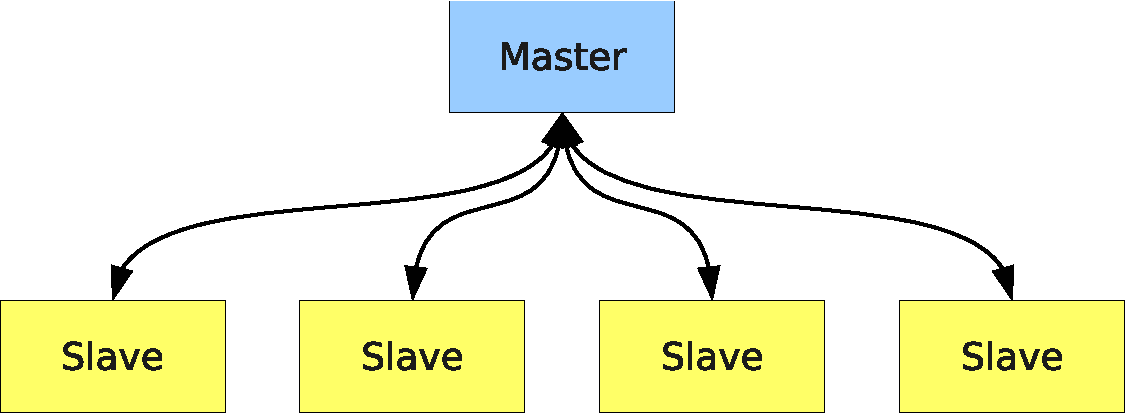
\includegraphics[width=0.8\textwidth]{figures/ch3/master-slave/master-slave.pdf}
  \caption{Typical master-slave algorithm.}
  \label{fig:master-slave}
\end{figure}
The most common parallel algorithm for fission source site sampling and
redistribution also relies on the master process for coordination --- doing so
makes it is easier to achieve reproducibility. In order to guarantee that the
process by which fission sites are randomly sampled does not depend on the
number of processors, the master-slave algorithm is typically implemented in the
following manner \cite{lanl-x5-2008}:
\begin{enumerate}
\item Each slave process \emph{sends} its fission bank sites to the master
  process. With $M$ fission sites in total distributed across the slave
  processes, this step can be completed in $O(M)$ time. Since $E[M] = N$, this
  implies that this step is $O(N)$.
\item The master process sorts or orders the fission sites based on a unique
  identifier. While a naïve sort would require $O(N \log N)$ steps on average,
  Brown outlines a reordering algorithm in \cite{trans-brown-1992} that can
  reduce this to $O(N)$.
\item The master process samples $N$ fission sites from the ordered array of $M$
  sites. This requires a loop over all fission sites and thus, by the same logic
  as before, is $O(N)$.
\item The master process \emph{broadcasts} all the fission sites to the slave
  processes. Since each slave process does not need to keep every source site in
  memory, one could modify the algorithm from a broadcast to a
  \emph{scatter}. However, for practical reasons (e.g. work self-scheduling
  \cite{lanl-brown-2005}), this is normally not done in production Monte Carlo
  codes. This step is also, at best, $O(N)$ as we will see later.
\end{enumerate}
The first and last steps of this algorithm involve communication between the
master and slave processes, whereas the second and third steps require
computation only on the master process. However, each of these steps is $O(N)$
at best. In practice, it is the network communication that becomes prohibitive
and prevents scalability, so we will thus focus our efforts on analyzing the
communication cost.

To estimate the communication cost of the master-slave algorithm, we will
introduce a simple latency-bandwidth model. In this model, we assume that the
time that it takes to send a message between two processes is given by $\alpha +
(dN)\beta$, where $\alpha$ is the time it takes to initiate the communication
(latency), $\beta$ is the transfer time per unit of data (inverse bandwidth),
$N$ is the number of fission sites, and $d$ is the size in bytes of each fission
site.

The first step of the master-slave algorithm is to send $p$ messages to the
master process, each of size $dN/p$ on average. Thus, the total time to send
these messages is
\begin{equation}
  \label{eq:t-send}
  t_{\text{send}} = p\alpha + dN\beta.
\end{equation}
Estimating the time of the broadcast is complicated by the fact that different
MPI implementations may use different algorithms to perform collective
communications. Worse yet, a single implementation may use a different algorithm
depending on how many processes are communicating and the size of the
message. Using multiple algorithms allows one to minimize latency for small
messages and minimize bandwidth for long messages.

We will focus here on the implementation of broadcast in the MPICH2
implementation \cite{ijhpca-mpich-2005}. For short messages, MPICH2 uses a
binomial tree algorithm. In this algorithm, the root process sends the data to
one process in the first step, and then in the subsequent step, both the root
and the other process can send the data to other processes. Thus, it takes a
total of $\lceil \log_2 p \rceil$ steps to complete the communication where
$\lceil x \rceil$ is the smallest integer not less than $x$. The time to
complete the communication is
\begin{equation}
  t_{\text{short}} = \lceil \log_2 p \rceil \left ( \alpha + dN\beta \right ).
\end{equation}
This algorithm works well for short messages since the latency term scales
logarithmically with the number of processes. However, for long messages, an
algorithm that has lower bandwidth has been proposed by Barnett et
al. \cite{sc-barnett-1994} and implemented in MPICH2. Rather than using a
binomial tree, the broadcast is divided into a scatter and an
\emph{allgather}. The time to complete the scatter is $ \log_2 p \: \alpha +
\frac{p-1}{p} N\beta$ using a binomial tree algorithm. The allgather is
performed using a ring algorithm that completes in $(p-1) \alpha + \frac{p-1}{p}
N\beta$. Thus, together the time to complete the broadcast is
\begin{equation}
  \label{eq:t-broadcast}
  t_{\text{long}} = \left ( \log_2 p + p - 1 \right ) \alpha + 2 \frac{p-1}{p}
  dN\beta.
\end{equation}
The fission bank data will generally exceed the threshold for switching from
short to long messages (typically 8 kilobytes), and thus we will use the
equation for long messages. Adding \eqref{eq:t-send} and \eqref{eq:t-broadcast},
we find the total cost of communication for the master-slave algorithm to be
\begin{equation}
  \label{eq:t-master-slave}
  t_{\text{master-slave}} = \left ( \log_2 p + 2p - 1 \right ) \alpha +
  \frac{3p-2}{p} dN\beta.
\end{equation}
For large $N$, it stands to reason that the communication will be
bandwidth-dominated. Based on the bandwidth term in \eqref{eq:t-master-slave},
we see that the combined communication requires $O(N)$ time.

\section{Nearest-Neighbor Algorithm}
\label{sec:nearest-neighbor}

To reduce the amount of communication required in a fission bank synchronization
algorithm, it is desirable to move away from the master-slave algorithm to a
nearest-neighbor algorithm whereby each process communicates only with other
processes that are logically adjacent in the network topology. This concept is
illustrated in \autoref{fig:nearest-neighbor}.
\begin{figure}[ht!]
  \centering
  
\includegraphics[width=0.9\textwidth]{figures/ch3/master-slave/nearest-neighbor.pdf}
  \caption{Nearest-neighbor communication pattern.}
  \label{fig:nearest-neighbor}
\end{figure}

Since the source sites for each fission generation are sampled from the fission
sites banked from the previous generation, it is common in the master-slave
algorithm for a fission site to be banked on one process, sent back to the
master, and finally sent back to the same process as a source site. As a result,
much of the communication inherent in the master-slave algorithm is entirely
unnecessary. By allowing each process to store and sample fission sites locally
and sending sites between processes only as needed, one can cut down on most of
the communication. The proposed algorithm to achieve this works as follows:
\begin{enumerate}
\item An exclusive scan is performed on the number of sites banked, and the
  total number of fission bank sites is broadcasted to all processes. By
  picturing the fission bank as one large array distributed across multiple
  processes, one can see that this step enables each process to determine the
  starting index of fission bank sites in this array. Let us call the starting
  and ending indices on the $i$th process $a_i$ and $b_i$, respectively;
\item Each process samples sites at random from the fission bank using the same
  starting seed. A separate array on each process is created that consists of
  sites that were sampled local to that process, i.e. if the index of the
  sampled site is between $a_i$ and $b_i$, it is set aside;
\item If $a_i$ is less than $iN/p$ where $N$ is the total number of particles
  per generation and $p$ is the number of processors, then send $iN/p - a_i$
  sites to the left adjacent process. Similarly, if $a_i$ is greater than
  $iN/p$, then receive $a_i - iN/p$ from the left adjacent process. This idea is
  applied to the fission bank sites at the end of each process' array as
  well. If $b_i$ is less than $(i+1)N/p$, then receive $(i+1)N/p - b_i$ sites
  from the right adjacent process. If $b_i$ is greater than $(i+1)N/p$, then
  send $b_i - (i+1)N/p$ sites to the right adjacent process. Thus, each process
  sends/receives only two messages under normal circumstances.
\end{enumerate}

The following example illustrates how this algorithm works. Let us suppose we
are simulating $N = 1,000$ particles distributed over four processes. For this
example, it is instructive to look at the state of the fission bank and source
bank at several points in the algorithm:
\begin{enumerate}
\item The beginning of a fission generation where each process has $N/p$ source
  sites;
\item The end of a fission generation where each process has accumulated fission
  sites;
\item After sampling, where each process has some amount of source sites usually
  not equal to $N/p$;
\item After redistribution, where each process again has $N/p$ source sites for
  the next cycle.
\end{enumerate}
At the end of each fission generation, each process needs $N/p = 250$ fission
bank sites to continue on the next generation. Suppose that process $p_0$
produces 270 fission banks sites, $p_1$ produces 230, $p_2$ produces 290, and
$p_3$ produces 250. After each process samples from its fission bank sites,
let's assume that $p_0$ has 260 source sites, $p_1$ has 215, $p_2$ has 280, and
$p_3$ has 245. For each process to have the same number of source sites, $p_0$
needs to send its right-most 10 sites to $p_1$, and $p_2$ needs to send its
left-most 25 sites to $p_1$ and its right-most 5 sites to $p_3$. A schematic of
this example is shown in \autoref{fig:nearest-neighbor-example}. The data local
to each process is given a different hatching, and the cross-hatched regions
represent source sites that are communicated between logically adjacent process.
\begin{figure}[ht!]
  \centering
  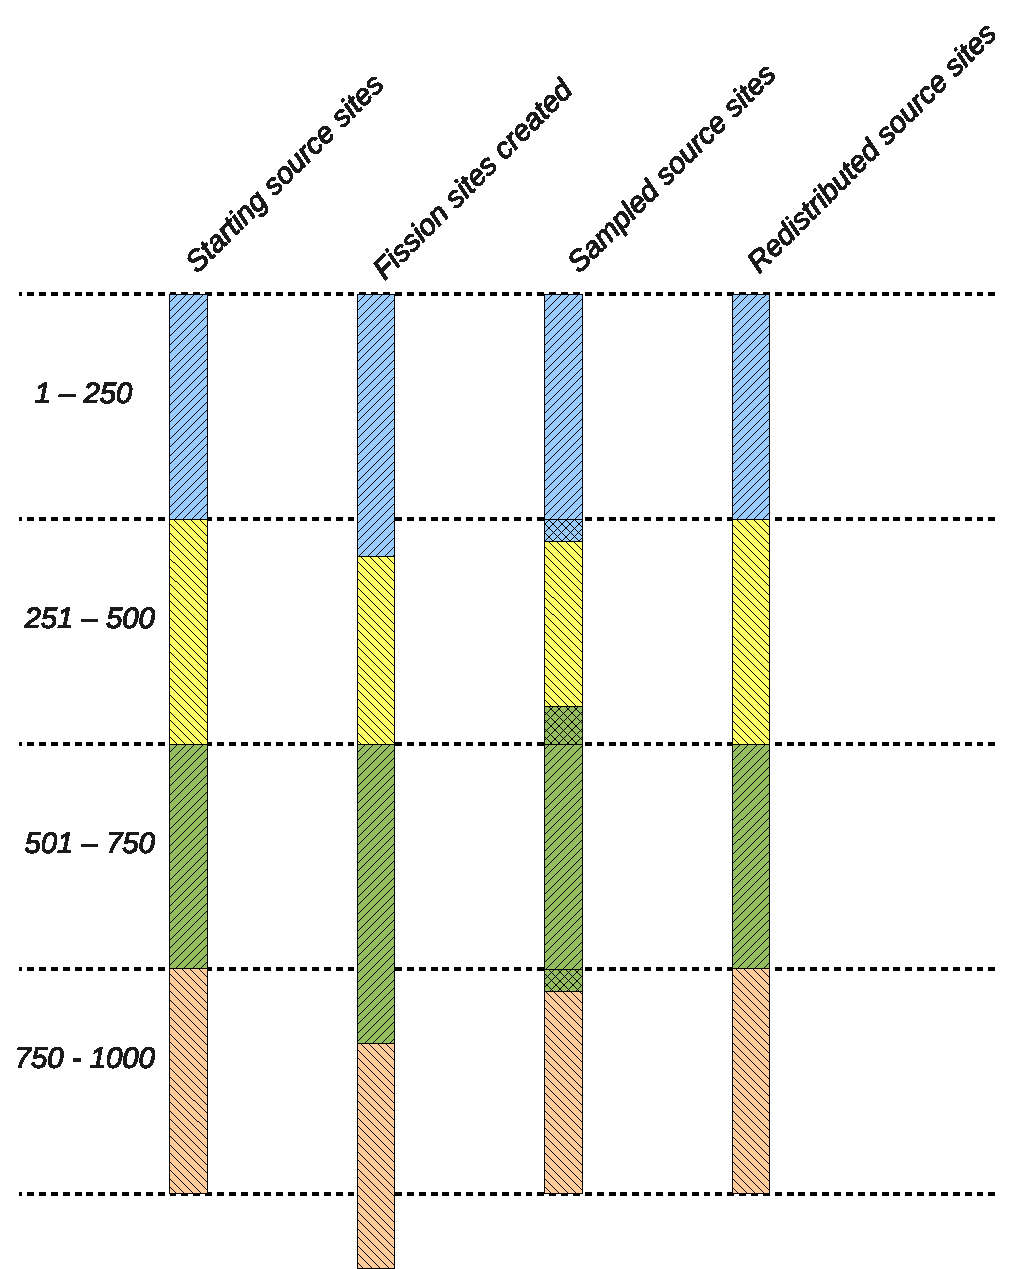
\includegraphics[width=0.9\textwidth]{figures/ch3/algorithm_schematic/nearest-neighbor-example.pdf}
  \caption{Example illustrating nearest-neighbor fission bank algorithm.}
  \label{fig:nearest-neighbor-example}
\end{figure}

Determining the expected communication cost of the nearest-neighbor algorithm is
not trivial due to the fact that the cost will be a function of how many fission
sites are sampled on each process. If each process samples exactly $N/p$ sites,
it would not be necessary to communicate any fission bank sites. However, if any
one process samples more or less than $N/p$ sites, the deviation will result in
communication between logically adjacent processes. To determine the expected
deviation, let us analyze the algorithm based on the fundamentals of the Monte
Carlo process.

The steady-state neutron transport equation for a multiplying medium can be
written in the form of an eigenvalue problem \cite{nukleonik-lieberoth-1968},
\begin{equation}
  \label{eq:NTE}
  S(\mathbf{r})= \frac{1}{k} \int F(\mathbf{r}' \rightarrow
  \mathbf{r})S(\mathbf{r}')\: d\mathbf{r},
\end{equation}
where $\mathbf{r}$ is the spatial coordinates of phase space, $S(\mathbf{r})$ is
the source distribution defined as the expected number of neutrons born from
fission per unit phase-space volume at $\mathbf{r}$, $F( \mathbf{r}' \rightarrow
\mathbf{r})$ is the expected number of neutrons born from fission per unit phase
space volume at $\mathbf{r}$ caused by a neutron at $\mathbf{r}'$, and $k$ is
the fundamental mode eigenvalue.

In a Monte Carlo eigenvalue calculation, the power iteration method is applied
iteratively to obtain stochastic realizations of the source distribution and
estimates of the $k$-eigenvalue. Let us define $\hat{S}^{(m)}$ to be the
realization of the source distribution at fission generation $m$ and
$\hat{\epsilon}^{(m)}$ to be the deviation from the deterministic solution
arising from the stochastic nature of the tracking process. We can write the
stochastic realization in terms of the fundamental source distribution and the
fluctuating component as \cite{ane-brissenden-1986}
\begin{equation}
  \label{eq:source}
  \hat{S}^{(m)}(\mathbf{r})= N S(\mathbf{r}) + \sqrt{N}
  \hat{\epsilon}^{(m)}(\mathbf{r}),
\end{equation}
where $N$ is the number of particle histories per generation. Without loss of
generality, we shall drop the superscript notation indicating the generation as
it is understood that the stochastic realization is at a particular
generation. The expected value of the stochastic source distribution is simply
\begin{equation}
  E \left[ \hat{S}(\mathbf{r})\right] = N S (\mathbf{r})
\end{equation}
since $E \left[ \hat{\epsilon}(\mathbf{r})\right] = 0$. The noise in the source
distribution is due only to $\hat{\epsilon}(\mathbf{r})$ and thus the variance
of the source distribution will be
\begin{equation}
  \text{Var} \left[ \hat{S}(\mathbf{r})\right] = N \text{Var} \left[
    \hat{\epsilon}(\mathbf{r}) \right].
\end{equation}
Lastly, the stochastic and true eigenvalues can be written as integrals over all
phase space of the stochastic and true source distributions, respectively, as
\begin{equation}
  \label{eq:k_to_source}
  \hat{k} = \frac{1}{N} \int \hat{S}(\mathbf{r}) \: d\mathbf{r} \quad \text{and}
  \quad k = \int S(\mathbf{r}) \: d\mathbf{r},
\end{equation}
noting that $S(\mathbf{r})$ is $O(1)$ since the true source distribution is not
a function of $N$ (see Nease et al. \cite{mc-nease-2009} for a thorough
discussion). One should note that the expected value $k$ calculated by Monte
Carlo power iteration (i.e. the method of successive generations) will be biased
from the true fundamental eigenvalue of \eqref{eq:NTE} by $O(1/N)$
\cite{ane-brissenden-1986}, but we will assume henceforth that the number of
particle histories per cycle is sufficiently large to neglect this bias.

With this formalism, we now have a framework within which we can determine the
properties of the distribution of expected number of fission sites. The explicit
form of the source distribution can be written as
\begin{equation}
  \hat{S}(\mathbf{r}) = \sum_{i=1}^{M} w_i \delta( \mathbf{r} - \mathbf{r}_i )
\end{equation}
where $\mathbf{r}_i$ is the spatial location of the $i$th fission site, $w_i$
is the statistical weight of the fission site at $\mathbf{r}_i$ (i.e. the weight
of the neutron entering into a fission reaction), and $M$ is the total number of
fission sites. It is clear that the total weight of the fission sites is simply
the integral of the source distribution. Integrating \eqref{eq:source} over all
space, we obtain
\begin{equation}
  \int \hat{S}(\mathbf{r}) \: d\mathbf{r} = N \int S(\mathbf{r}) \: d\mathbf{r}
  + \sqrt{N} \int \hat{\epsilon}(\mathbf{r}) \: d\mathbf{r} .
\end{equation}
Substituting the expressions for the stochastic and true eigenvalues from
\eqref{eq:k_to_source}, we can relate the stochastic eigenvalue to the integral
of the noise component of the source distribution as
\begin{equation}
  N\hat{k} = Nk + \sqrt{N} \int \hat{\epsilon}(\mathbf{r}) \: d\mathbf{r}.
\end{equation}
Since the expected value of $\hat{\epsilon}$ is zero, the expected value of its
integral will also be zero. We thus see that the variance of the integral of the
source distribution, i.e. the variance of the total weight of fission sites
produced, is directly proportional to the variance of the integral of the noise
component. Let us call this term $\sigma^2$ for simplicity:
\begin{equation}
  \text{Var} \left[ \int \hat{S}(\mathbf{r}) \: d\mathbf{r} \right ] = N
  \sigma^2.
\end{equation}
The actual value of $\sigma^2$ will depend on the physical nature of the
problem, whether variance reduction techniques are employed, etc. For instance,
one could surmise that for a highly scattering problem, $\sigma^2$ would be
smaller than for a highly absorbing problem since more collisions will lead to a
more precise estimate of the source distribution. Similarly, using survival
biasing should in theory reduce the value of $\sigma^2$.

Let us now consider the case where the $N$ total histories are divided up evenly
across $p$ processes. Since each process simulates $N/p$ histories, we can write
the source distribution as
\begin{equation}
  \hat{S}_i(\mathbf{r})= \frac{N}{p} S(\mathbf{r}) + \sqrt{\frac{N}{p}}
  \hat{\epsilon}_i(\mathbf{r}) \quad \text{for} \quad i = 1, \dots, p
\end{equation}
Integrating over all space and simplifying, we can obtain an expression for the
eigenvalue on the $i$th process:
\begin{equation}
  \hat{k}_i = k + \sqrt{\frac{p}{N}} \int \hat{\epsilon}_i(\mathbf{r}) \:
  d\mathbf{r}.
\end{equation}
It is easy to show from this expression that the stochastic realization of the
global eigenvalue is merely the average of these local eigenvalues:
\begin{equation}
  \label{eq:average_k_as_sum}
  \hat{k} = \frac{1}{p} \sum_{i=1}^p \hat{k}_i.
\end{equation}
As was mentioned earlier, at the end of each generation one must sample $N$
sites from the $M$ sites that were created. Thus, the source for the next
generation can be seen as the fission source from the current generation divided
by the stochastic realization of the eigenvalue since it is clear from
\eqref{eq:k_to_source} that $\hat{k} = M/N$. Similarly, the number of sites
sampled on each process that will be used for the next generation is
\begin{equation}
  \label{eq:sites_per_node}
  M_i = \frac{1}{\hat{k}} \int \hat{S}_i(\mathbf{r}) \: d\mathbf{r} =
  \frac{N}{p} \frac{\hat{k}_i}{\hat{k}}.
\end{equation}

While we know conceptually that each process will under normal circumstances
send two messages, many of these messages will overlap. Rather than trying to
determine the actual communication cost, we will instead attempt to determine
the maximum amount of data being communicated from one process to another. At
any given generation, the number of fission sites that the $j$th process will
send or receive, $\Lambda_j$, is
\begin{equation}
  \label{eq:Lambda}
  \Lambda_j = \left | \sum_{i=1}^j M_i - \frac{jN}{p} \right |.
\end{equation}
Noting that $jN/p$ is the expected value of the summation, we can write the
expected value of $\Lambda_j$ as the mean absolute deviation of the summation:
\begin{equation}
  E \left [ \Lambda_j \right ] = E \left [ \left | \sum_{i=1}^j M_i -
    \frac{jN}{p} \right | \right ] = \text{MD} \left [ \sum_{i=1}^j M_i \right ]
\end{equation}
where $\text{MD}$ indicates the mean absolute deviation of a random
variable. The mean absolute deviation is an alternative measure of variability.

In order to ascertain any information about the mean deviation of $M_i$, we need
to know the nature of its distribution. Thus far, we have said nothing of the
distributions of the random variables in question. The total number of fission
sites resulting from the tracking of $N$ neutrons can be shown to be normally
distributed via the Central Limit Theorem (provided that $N$ is sufficiently
large) since the fission sites resulting from each neutron are ``sampled'' from
independent, identically-distributed random variables. Thus, $\hat{k}$ and $\int
\hat{S} (\mathbf{r}) \: d\mathbf{r}$ will be normally distributed as will the
individual estimates of these on each process.

Next, we need to know what the distribution of $M_i$ in
\eqref{eq:sites_per_node} is or, equivalently, how $\hat{k}_i / \hat{k}$ is
distributed. The distribution of a ratio of random variables is not easy to
calculate analytically, and it is not guaranteed that the ratio distribution is
normal if the numerator and denominator are normally distributed. For example,
if $X$ is a standard normal distribution and $Y$ is also standard normal
distribution, then the ratio $X/Y$ has the standard Cauchy distribution. The
reader should be reminded that the Cauchy distribution has no defined mean or
variance. That being said, Geary \cite{jrss-geary-1930} has shown that, for the
case of two normal distributions, if the denominator is unlikely to assume
values less than zero, then the ratio distribution is indeed approximately
normal. In our case, $\hat{k}$ absolutely cannot assume a value less than zero,
so we can be reasonably assured that the distribution of $M_i$ will be normal.

For a normal distribution with mean $\mu$ and distribution function $f(x)$, it
can be shown that
\begin{equation}
  \int_{-\infty}^{\infty} f(x) \left | x - \mu \right | \: dx =
  \sqrt{\frac{2}{\pi} \int_{-\infty}^{\infty} f(x) \left ( x - \mu \right )^2 \:
    dx}
\end{equation}
by substituting the probability distribution function of a normal distribution
for $f(x)$, making a change of variables, and integrating both sides. Thus the
mean absolute deviation is $\sqrt{2/\pi}$ times the standard
deviation. Therefore, to evaluate the mean absolute deviation of $M_i$, we need
to first determine its variance. Substituting \eqref{eq:average_k_as_sum} in
\eqref{eq:sites_per_node}, we can rewrite $M_i$ solely in terms of $\hat{k}_1,
\dots, \hat{k}_p$:
\begin{equation}
  M_i = \frac{N \hat{k}_i}{\sum\limits_{j=1}^p \hat{k}_j}.
\end{equation}
Since we know the variance of $\hat{k}_i$, we can use the error propagation law
to determine the variance of $M_i$:
\begin{equation}
  \text{Var} \left [ M_i \right ] = \sum_{j=1}^p \left ( \frac{\partial
    M_i}{\partial \hat{k}_j} \right )^2 \text{Var} \left [ \hat{k}_j \right ] +
  \sum\limits_{j \neq m} \sum\limits_{m=1}^p \left ( \frac{\partial
    M_i}{\partial \hat{k}_j} \right ) \left ( \frac{\partial M_i}{\partial
    \hat{k}_m} \right ) \text{Cov} \left [ \hat{k}_j, \hat{k}_m \right ]
\end{equation}
where the partial derivatives are evaluated at $\hat{k}_j = k$. Since
$\hat{k}_j$ and $\hat{k}_m$ are independent if $j \neq m$, their covariance is
zero and thus the second term cancels out. Evaluating the partial derivatives,
we obtain
\begin{equation}
  \text{Var} \left [ M_i \right ] = \left ( \frac{N(p-1)}{kp^2} \right )^2
  \frac{p\sigma^2}{N} + \sum_{j \neq i} \left ( \frac{-N}{kp^2} \right )^2
  \frac{p\sigma^2}{N} = \frac{N(p-1)}{k^2p^2} \sigma^2.
\end{equation}
Through a similar analysis, one can show that the variance of $\sum_{i=1}^j M_i$
is
\begin{equation}
  \text{Var} \left [ \sum_{i=1}^j M_i \right ] = \frac{Nj(p-j)}{k^2p^2} \sigma^2
\end{equation}
Thus, the expected amount of communication on process $j$, i.e. the mean
absolute deviation of $\sum_{i=1}^j M_i$, is proportional to
\begin{equation}
  \label{eq:comm-cost}
  E \left [ \Lambda_j \right ] = \sqrt{\frac{2Nj(p-j)\sigma^2}{\pi k^2p^2}}.
\end{equation}
Equation \eqref{eq:comm-cost} has all the properties that one would expect based
on intuition:
\begin{itemize}
\item As the number of particle histories increases, the communication cost on
  each process increases as well;
\item If $p=1$, i.e. if the problem is run on only one process, the variance
  will be zero. This reflects the fact that exactly $N$ sites will be sampled if
  there is only one process.
\item For $j=p$, the variance will be zero. Again, this says that when you sum
  the number of sites from each process, you will get exactly $N$ sites.
\end{itemize}
We can determine the process that has the highest communication cost by
differentiating \eqref{eq:comm-cost} with respect to $j$, setting it equal to
zero, and solving for $j$. Doing so yields $j_{\text{max}} =
p/2$. Interestingly, substituting $j = p/2$ in \eqref{eq:comm-cost} indicates
that the maximum communication cost is actually independent of the number of
processes:
\begin{equation}
  \label{eq:nn-cost-max}
  E \left [ \Lambda_{j_{\text{max}}} \right ] = \sqrt{ \frac{N\sigma^2}{2\pi
      k^2}}.
\end{equation}

We can now proceed as before and estimate the communication time using the
latency-bandwidth model. As discussed earlier, each process should send or
receive only two messages, one to each of its neighbors. Since the largest
message will occur on process $j_{\text{max}} = p/2$, we can use
\eqref{eq:nn-cost-max} and \eqref{eq:t-send} to estimate the communication time
for the nearest-neighbor algorithm as
\begin{equation}
  \label{eq:t-nearest-neighbor}
  t_{\text{nearest-neighbor}} = 2\alpha + d\sqrt{\frac{2N\sigma^2}{\pi k^2}} \beta
\end{equation}
To compare the communication time of the two algorithms, we can assume that the
message size is large enough that the communication will be bandwidth
dominated. Dividing \eqref{eq:t-master-slave} by \eqref{eq:t-nearest-neighbor},
we find that
\begin{equation}
  \frac{t_{\text{master-slave}}}{t_{\text{nearest-neighbor}}} = \frac{\left (
    \log_2 p + 2p - 1 \right ) \alpha + \frac{3p-2}{p} dN\beta}{2\alpha +
    d\sqrt{\frac{2N\sigma^2}{\pi k^2}} \beta} \approx \frac{ \left ( 3p - 2
    \right ) k \sqrt{N\pi/2}}{ p\sigma }.
\end{equation}
In the limit of large $p$, this ratio becomes
\begin{equation}
  \label{eq:t-ratio-limit}
  \lim_{p\rightarrow\infty}
  \frac{t_{\text{master-slave}}}{t_{\text{nearest-neighbor}}} =
  \sqrt{\frac{N\pi}{2}} \cdot \frac{3k}{\sigma}.
\end{equation}

We can see from \eqref{eq:t-nearest-neighbor} that the nearest-neighbor
algorithm requires $O(\sqrt{N})$ time instead of $O(N)$ as for the master-slave
algorithm. This should allow the the algorithm to scale to very large numbers of
total processes or particles per generation. In fact, we can show that
arbitrarily good scaling can be achieved. Let $t$ be the time to simulate $N$
particles on $p$ processors. Expressing the network communication time as a
fraction of the time to simulate the particles, we find that:
\begin{equation}
  \frac{t_{\text{nearest-neighbor}}}{t} \propto \frac{\sqrt{N}}{N/p} \propto
  \frac{p}{\sqrt{N}}
\end{equation}
Thus, if we keep $p$ constant and increase $N$, the relative time to complete
network communication will be reduced since the simulation time is proportional
to $N$ and the communication is proportional to $\sqrt{N}$.

\section{Validation of Theoretical Analysis}
\label{sec:fission-bank-validation}

To ensure that any assumptions made in the foregoing analysis are sound, several
test cases using an implementation of the nearest-neighbor fission bank
algorithm in OpenMC were run to provide results that can be compared with the
theoretical analysis. The number of processes and particle histories for each
case are shown in \autoref{tab:cases}.
\begin{table}[ht!]
  \centering
  \caption{Test cases for nearest-neighbor fission bank algorithm.}
  \label{tab:cases}
  \begin{tabular}{ c c c }
    \toprule
    Case & Processes ($p$) & Histories ($N$) \\ 
    \midrule
    1 & 8 & 80,000 \\
    2 & 8 & 160,000 \\
    3 & 16 & 80,000 \\
    4 & 16 & 160,000 \\
    \bottomrule
  \end{tabular}
\end{table}
Each case was run for 10,000 generations and at the end of each run, the
standard deviation of the number of fission bank sites sent to logically
adjacent processes was determined for each process as a proxy for the
communication cost. For Case 1, the data were fit to the following function
(with the same dependence on $j$ and $p$ as in \eqref{eq:comm-cost}) using a
least squares regression:
\begin{equation}
  \label{eq:regression}
  f(j,p,\beta) = \frac{\beta}{p} \sqrt{j(p-j)}.
\end{equation}
The fitting coefficient $\beta$ was then used to predict the expected amount of
communication for the other three cases. \autoref{fig:mean-deviance8} shows the
expected number of fission bank sites sent or received from neighboring
processes, $E \left [ \Lambda_j \right ]$, for Cases 1 and 2 along with the
least squares regression fit based on \eqref{eq:regression} for Case 1 and the
prediction for Case 2. \autoref{fig:mean-deviance16} shows the expected number
of fission bank sites sent or received from neighboring processes for Cases 3
and 4 along with the predicted fits.
\begin{figure}[ht!]
  \centering
  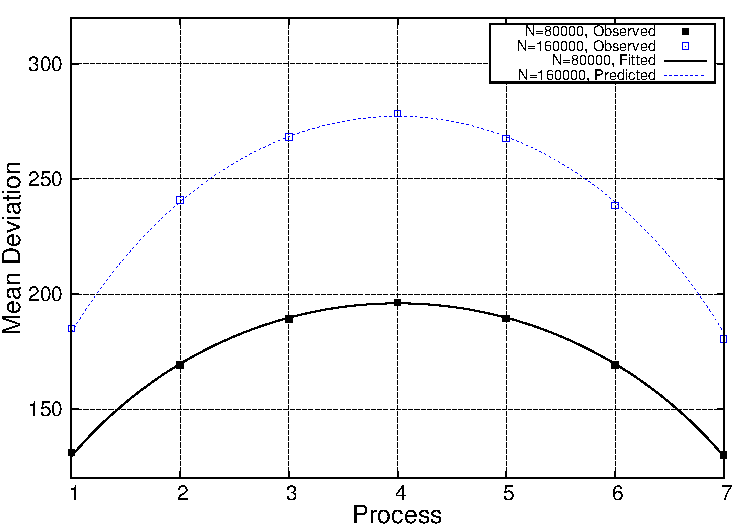
\includegraphics[width=0.75\textwidth]{figures/ch3/mean_deviance/plot8.pdf}
  \caption{Expected number of fission bank sites sent to neighboring processes
    using 8 processes.}
  \label{fig:mean-deviance8}
\end{figure}
\begin{figure}[ht!]
  \centering
  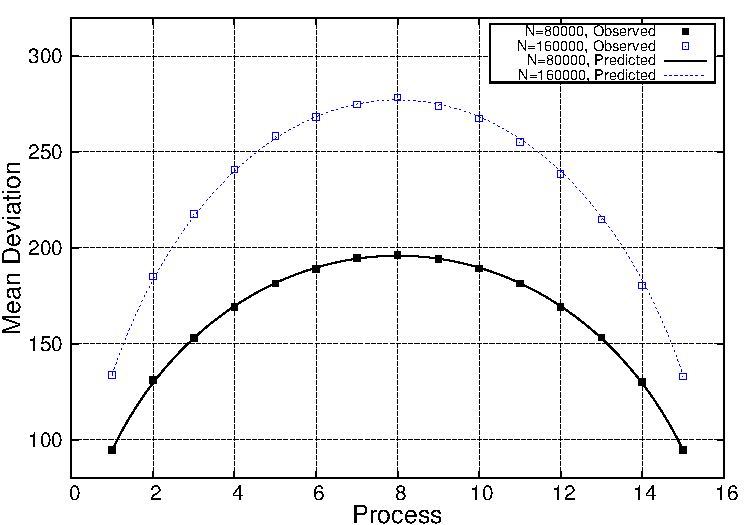
\includegraphics[width=0.75\textwidth]{figures/ch3/mean_deviance/plot16.pdf}
  \caption{Expected number of fission bank sites sent to neighboring processes
    using 16 processes.}
  \label{fig:mean-deviance16}
\end{figure}
A few observations can be made from these figures. Firstly, the data from the
four test cases demonstrates that the foregoing theoretical analysis is indeed
correct. Furthermore, one can observe from these two figures that the maximum
communication does occur for process $j_{\text{max}} = p/2$ and that this
maximum is independent of $p$ as predicted.

It is also instructive to check our assumption that $\sum_{i=1}^j M_i$ is
normally distributed. One way of doing this is through a quantile-quantile (Q-Q)
plot, comparing the observed quantiles of the data with the theoretical
quantiles of the normal distribution. If the data are normally distributed, the
points on the Q-Q plot should lie along a line. \autoref{fig:QQ-plot} shows a
Q-Q plot for the number of fission bank sites sent or received on the first
process for Case 1.
\begin{figure}[ht!]
  \centering
  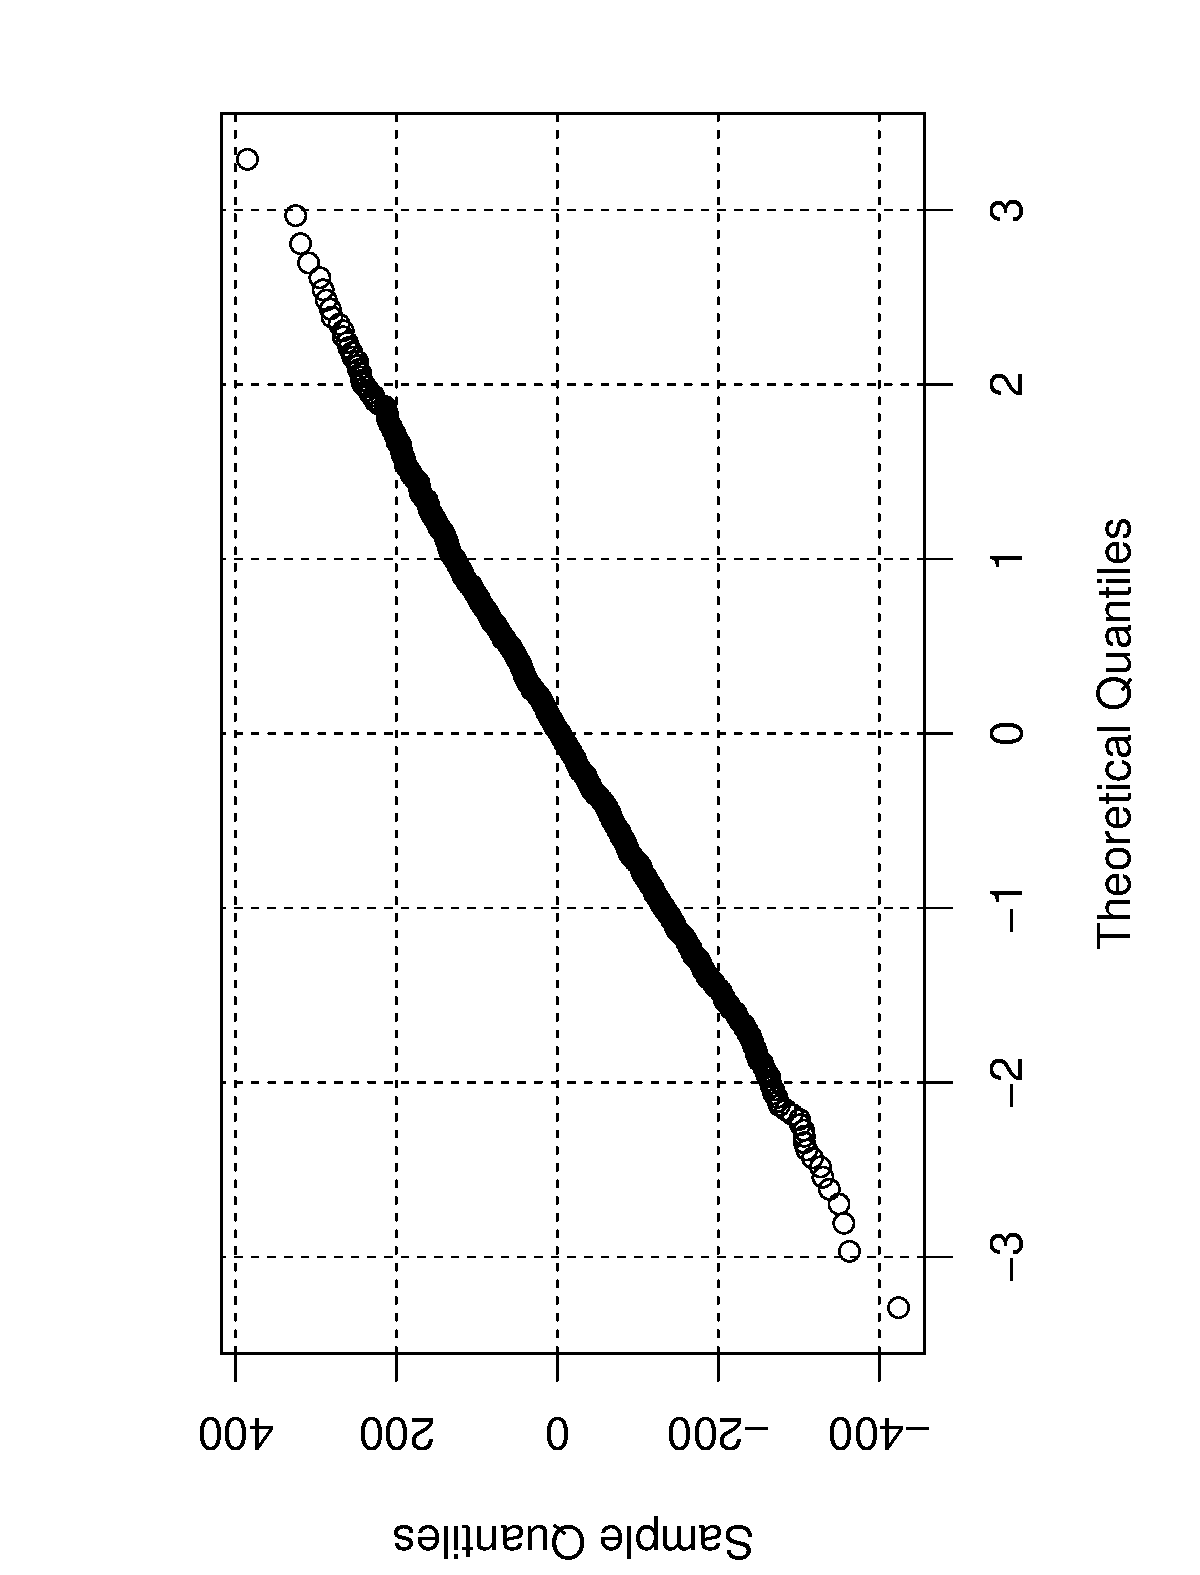
\includegraphics[width=0.75\textwidth,angle=-90]{figures/ch3/QQ_plot/QQplot.pdf}
  \caption{Q-Q plot of $M_1$ for Case 1}
  \label{fig:QQ-plot}
\end{figure}
The data clearly lie along a straight line and thus the data are normally
distributed. This conclusion was also confirmed using the Shapiro-Wilk test for
normality \cite{biometrika-shapiro-1965}.

\section{Results}
\label{sec:fission-bank-results}

\subsection{Communication Time}

In \autoref{sec:nearest-neighbor}, it was shown that the communication cost of
nearest neighbor algorithm will depend on a parameter $\sigma$ representing the
variance in the number of sites sent between adjacent processes. Thus, while we
can conclude from \eqref{eq:t-ratio-limit} that the nearest-neighbor algorithm
will certainly outperform the master-slave algorithm in the limit of large $p$
and $N$, it is more difficult to make inferences regarding the performance of
the two algorithms for smaller cases.

In order to compare the two algorithms, both were implemented in OpenMC. A
separate simulation using each of the algorithms was run from a single process
up to 88 processes in parallel on a small cluster with an Ethernet network
interconnect. In each case, the number of histories was 40,000 times the number
of processes so that each process simulates the same number of histories. Each
simulation was run for 20 fission generations. \autoref{fig:algorithm-time}
shows the total time spent on fission bank synchronization for the two
algorithms.
\begin{figure}[ht!]
  \centering
  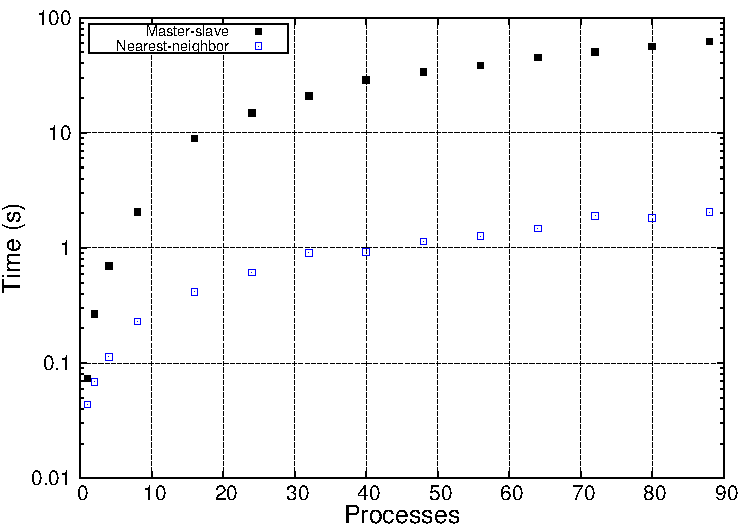
\includegraphics[width=0.75\textwidth]{figures/ch3/algorithm_results/time.pdf}
  \caption{Execution time for fission bank algorithms.}
  \label{fig:algorithm-time}
\end{figure}
We see that the the nearest-neighbor algorithm performs nearly two orders of
magnitude faster than the master-slave algorithm for large $p$ and large $N$. In
these simulations, we have ignored the time spent sampling fission sites and
copying data in memory which may become non-negligible for large $N$. Thus, to
truly demonstrate scalability, simulations with much larger $N$ and $p$ are
needed.

\subsection{Parallel Scaling}

To test parallel scaling, an OpenMC model of the Monte Carlo Performance
Benchmark was simulated on both the Blue Gene/P at the Argonne Leadership
Computing Facility (Intrepid) and the Cray XK6 at the Oak Ridge Leadership
Computing Facility (Jaguar) using the nearest-neighbor fission bank
algorithm. On the Blue Gene/P, up to 163,840 cores were used with 4000 particles
per processor core per generation. On the Cray XK6, up to 131,072 cores were
used with 20,000 particles per processor core per generation. For this study,
the total work per processor was kept constant (weak scaling) rather than the
total amount of work over all processors (strong scaling). \autoref{fig:scaling}
shows the effective number of particles simulated per second as a function of
the number of processors in comparison to the ideal calculation rate (assuming
no communication between fission source iterations). Excellent parallel
efficiency is achieved even above 100,000 processors.
\begin{figure}[ht]
  \centering
  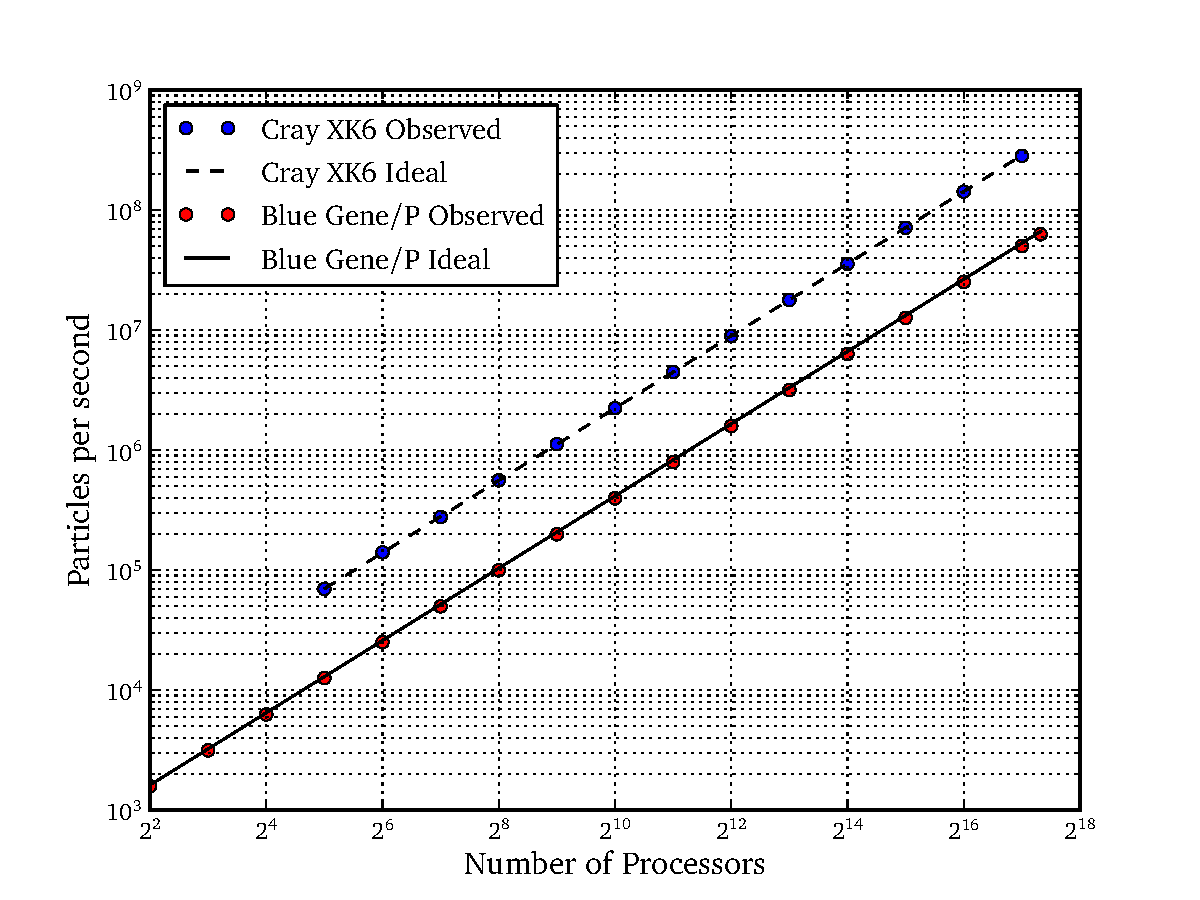
\includegraphics[width=0.9\textwidth]{figures/ch3/scaling/scaling_loglog.pdf}
  \caption{Parallel scaling for the Monte Carlo Performance Benchmark on the
    Cray XK6 (Jaguar) and Blue Gene/P (Intrepid) supercomputers.}
  \label{fig:scaling}
\end{figure}

A few notes should be made regarding the achieved scaling shown in
\autoref{fig:scaling}. First, it was necessary to use non-blocking communication
semantics rather than blocking communication; when blocking communication was
attempted, the scaling behavior was observed to be much worse. Additionally, it
was necessary to turn off the calculation of Shannon entropy during the
simulations. In OpenMC, the number of mesh cells used for the Shannon entropy
mesh grows linearly with the number of particles per generation. At the end of
the fission generation, the number of source sites in each mesh cell has to be
reduced from all processes before being used in \eqref{eq:shannon-entropy}. As
such, in a series of weak scaling runs, the communication associated with
calculating Shannon entropy would grow linearly with the number of processors
--- turning off the calculation of Shannon entropy circumvents this.

\section{Other Considerations}
\label{sec:fission-bank-other}

\subsection{Load Balancing}

One important requirement for a parallel Monte Carlo calculation is proper
load-balancing, i.e. it is undesirable to have a process sitting idle with no
work to do while other processes are still busy working. This is especially the
case when the hardware architecture is heterogeneous (having different types of
processors in a single cluster). In the master-slave algorithm, work
self-scheduling is achieved by having each slave process request small batches
of work from the master, and as each batch is completed, the slave may request
more work. By breaking up the problem into smaller batches, this ensures that in
a single source iteration, a processor that is twice as fast as another
processor will also be assigned twice as many histories to compute, and thus all
processors should finish their work at approximately the same time.

The nearest-neighbor algorithm unfortunately precludes the use of the
aforementioned self-scheduling algorithm since an important aspect of the
algorithm is to assign particle histories sequentially to the processes to
preserve their order. It should be noted that if one did not care to preserve
reproducibility in a calculation, the self-scheduling scheme could easily be
applied for load-balancing with the nearest-neighbor fission bank algorithm.

The results in \autoref{fig:scaling} demonstrate that the lack of a load
balancing mechanism does not degrade parallel efficiency when used on a
homogeneous cluster. Previous studies using MCNP on a homogeneous Linux cluster
have shown a 5-10\% loss in parallel efficiency when not using any sort of load
balancing \cite{lanl-brown-2005}.

It is also possible to employ a basic means of load balancing for heterogeneous
architectures using in the nearest-neighbor algorithm by ``tuning'' the
algorithm to the specific characteristics of the cluster. If one were to measure
the performance of each type of processor on the cluster in terms of particles
processed per second, the number of histories on each processor could be
adjusted accordingly instead of merely distributing particles uniformly ($N/p$
on each processor).

\subsection{Fault Tolerance}

For petascale and future exascale architectures, it is desirable to have some
means of fault tolerance to ensure that not all results are lost in the event of
a hardware failure. In current Monte Carlo codes, this can be achieved by having
all processes periodically rendezvous and collectively dump data to a file that
can be used to restart the run. While providing insurance against lost
simulation time, performing fault tolerance this way unfortunately degrades
parallel performance since it entails collective communication between all
processors. Notwithstanding, the algorithm we have presented here does not
inhibit the use of fault tolerance in this manner.

\section{Conclusions}
\label{sec:conclusions}

In this chapter, we presented a new algorithm for parallelizing the source
iterations in a Monte Carlo criticality calculation. This algorithm takes
advantage of the fact that many of the fission sites produced on one processor
can be used as source sites on that same processor --- in doing so, it avoids
unnecessary communication between processors.

Analysis of the algorithm shows that it should outperform existing algorithms
for fission bank synchronization and that furthermore, the performance gap
increases for an increasing number of histories or processors. Test results on
the OpenMC Monte Carlo code confirm this finding. The analysis also shows that
the maximum amount of communication in the algorithm is independent of the
number of processors and instead will depend on the number of histories per
cycle and the physical characteristics of the problem at hand. Again, testing
within OpenMC confirms this prediction. Finally, a scaling study was performed
on the Titan and Intrepid supercomputers and demonstrated perfect scaling with
over 100,000 processor cores using the nearest-neighbor algorithm.

The reader should keep in mind that while the algorithm presented here will
significantly improve the time necessary to sample and distribute fission sites
between cycles, it has no effect on the actual transport simulation of particles
moving through a material medium. Thus, it will not improve smaller simulations
that would typically run on a workstation. However, for large simulations that
necessitate the use of a large cluster or supercomputer to complete in a
reasonable amount of time, this novel algorithm will improve the parallel
efficiency and is an important step in achieving scalability up to thousands or
millions of processors.

One potential shortcoming of the present algorithm is that it precludes the use
of load balancing via existing algorithms for heterogeneous computer
architectures. A basic method to provide load balancing in such situations based
on ``tuning'' the algorithm was suggested, although it has not yet been tested.

\chapter{Tally Reduction Algorithms}
\label{chap:tally-reduction}

In \autoref{chap:fission-bank}, a nearest-neighbor fission bank algorithm was
proposed, implemented in OpenMC, and demonstrated to enable parallel scaling in
Monte Carlo $k$-eigenvalue calculations with over 100,000 processors. While this
algorithm is an important and necessary component in being able to perform
realistic LWR analysis with Monte Carlo methods, it is only one piece of the
puzzle. We had also identified in \autoref{chap:intro} that large tallies can
become problematic in large-scale parallel simulations due to excessive
communication requirements. In fact, in the scaling study in
\autoref{sec:fission-bank-results}, no tallies were included in the runs, and
hence the necessary network communication was greatly reduced.

In this chapter, we propose a method that would greatly reduce network
communication when performing parallel simulations with large tally data by
using statistical batching across fission generations. In
\autoref{sec:batch-statistics}, we first review batch statistics and their
current utility in Monte Carlo simulations. A modified batching algorithm is
then proposed and analyzed in \autoref{sec:tally-reduction}. The Monte Carlo
performance benchmark was simulated using an implementation of the algorithm in
OpenMC; the results of these tests are reported in
\autoref{sec:tally-reduction-results}.

The algorithm being presented in this chapter was published in an article in
\emph{Transactions of the American Nuclear Society} \cite{trans-romano-2012}.

%%%%%%%%%%%%%%%%%%%%%%%%%%%%%%%%%%%%%%%%%%%%%%%%%%%%%%%%%%%%%%%%%%%%%%%%%%%%%%%%
\section{Batch Statistics}
\label{sec:batch-statistics}

To construct an estimate for the sample mean and its variance for any tally in a
Monte Carlo simulation, the following formulas are generally used:
\begin{align}
  \bar{x} &= \frac{1}{N} \sum_{i=1}^N x_i \\ 
  \label{eq:variance-mean} s^2_{\bar{x}} &= \frac{1}{N-1}
  \left [ \frac{\sum_{i=1}^N x_i^2}{N} - \left ( \frac{\sum_{i=1}^N x_i}{N}
    \right )^2 \right ]
\end{align}
where $x_i$ is a single realization of the random variable, $\bar{x}$ is the
sample mean, $s^2_{\bar{x}}$ is the variance of the sample mean, and $N$ is the
number of realizations. A single realization may be the accumulated score from a
single particle history in a fixed-source calculation or from a single fission
generation in a criticality calculation. A few assumptions have been made in the
use of \eqref{eq:variance-mean}; it is assumed that $N$ is large enough for the
law of large numbers and the central limit theorem (CLT) to apply, and it is
assumed that the realizations were drawn from independent and identically
distributed random variables, again to satisfy conditions of the CLT.

In the method of successive generations used for Monte Carlo eigenvalue
calculations, the locations of source sites in one generation may be correlated
with the locations of source sites in a subsequent generation. This is
especially true in problems where the overall dimensions of the problem are
large relative to the mean free path of neutrons. The correlation between
fission sites also results in a correlation between realizations of tally random
variables. Unfortunately, this correlation is not accounted for in
\eqref{eq:variance-mean}. As a result, in problems where there is significant
correlation between successive generations (equivalently, in problems with high
dominance ratios), using \eqref{eq:variance-mean} to calculate the variance of
the sample mean can result in underprediction of the true variance, and hence
underprediction of confidence interval width for tallies.

Various solutions to the underprediction of true variance have been been studied
in the literature. One of the simpler solutions proposed is to simply treat the
accumulated scores from multiple fission generations, referred to as a
\emph{batch}\footnote{Many people use the terms ``batch'', ``generation'', and
  ``cycle'' interchangeably. In this paper, the term ``batch'' specifically
  refers to the grouping of multiple realizations and is generally not the same
  as a ``generation'' or ``cycle'' in a criticality calculation.}, as a single
realization of a tally random variable \cite{pne-gelbard-1990}. Mathematically,
grouping $M$ successive realizations, $x_i, i = 1,\dots,M$, of a random variable
yields a separate estimate of a new random variable:
\begin{equation}
  y_j = \sum_{i=(j-1)M + 1}^{jM} x_i.
\end{equation}
We note that $M$ must be sufficiently large for the central limit theorem to
apply to the distribution of $y_j$, i.e. the batch must be large enough to
sufficiently reduce correlation between successive batches. The sample mean and
its variance for the new random variable are then
\begin{align}
  \bar{y} &= \frac{1}{N'} \sum_{j=1}^{N'} y_j \\ s^2_{\bar{y}} &= \frac{1}{N'-1}
  \left [ \frac{\sum_{j=1}^{N'} y_j^2}{N'} - \left ( \frac{\sum_{j=1}^{N'} y_j}{N'}
    \right )^2 \right ]
\end{align}
where $N' = N/M$. It is obvious by inspection that the sample mean $\bar{x}$ and
$\bar{y}$ will have the same value regardless of the batching
strategy. Furthermore, while the variances will in general be different, it can
be shown that the expected value of the variances $s^2_{\bar{x}}$ and
$s^2_{\bar{y}}$ are the same. The use of batches provides two main benefits:
\begin{enumerate}
  \item If $M$ is large enough, the random variables that result from the
    batching process are guaranteed to be normally distributed as per the
    central limit theorem.
  \item With a large enough batch size, the correlation between successive
    realizations of the tally random variables becomes negligible, thus ensuring
    that the true variance is not underestimated.
\end{enumerate}
This method has been implemented and successfully utilized in the MC21 Monte
Carlo code \cite{physor-kelly-2012}.

\section{Reduction of Tally Scores}
\label{sec:tally-reduction}

Now let us focus our attention on a situation whereby we are performing a Monte
Carlo simulation on $p$ processors with the entire geometry of the problem
replicated on each processor. After each realization, every processor has its
own accumulated score for the tally variable $x_{i,k}$ where $k$ denotes the
$k$th processor. Traditionally, to obtain the same answer as would be obtained
in a serial calculation, we would need to take the summation of the tallies
across all processors at the end of the realization, i.e. $x_i = \sum_{k=1}^p
x_{i,k}$. This is depicted in \autoref{fig:history} where scores inside each box
are summed into a single realization.
\begin{figure}[ht]
  \centering
  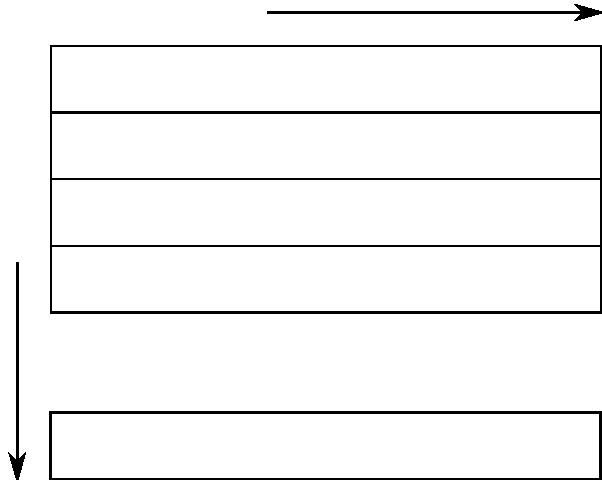
\includegraphics[width=3in]{figures/ch4/history.pdf}
  \caption{Summation of tally scores across processors when doing statistics
    based on a single particle history or single generation.}
  \label{fig:history}
\end{figure}
In terms of network communication, we will need to send at a minimum 8 bytes for
each of the $\ell$ tally bins on $p-1$ processors to the master
process\footnote{This is typically done with the Message Passing Interface by
  calling MPI\_REDUCE.}. Thus, the total amount of data that must be
communicated during the simulation is $8\ell N (p-1)$ bytes since the summation
must be done at every realization. For a simulation with large $\ell$ and/or
large $p$, the time to perform this communication can become prohibitive. An
example of such a scenario is the calculation of the global power distribution
in a large reactor model using a cluster or supercomputer, a calculation easily
requiring millions of tally bins, if not more.

Performing statistics over a batch consisting of multiple realizations somewhat
alleviates the communication requirements while providing other aforementioned
benefits. The summation of tally scores for this scenario is depicted in
\autoref{fig:batch}. Since the reduction now need only be performed at the end
of a batch, the data requirement is then $8\ell N' (p-1)$.
\begin{figure}[htb]
  \centering
  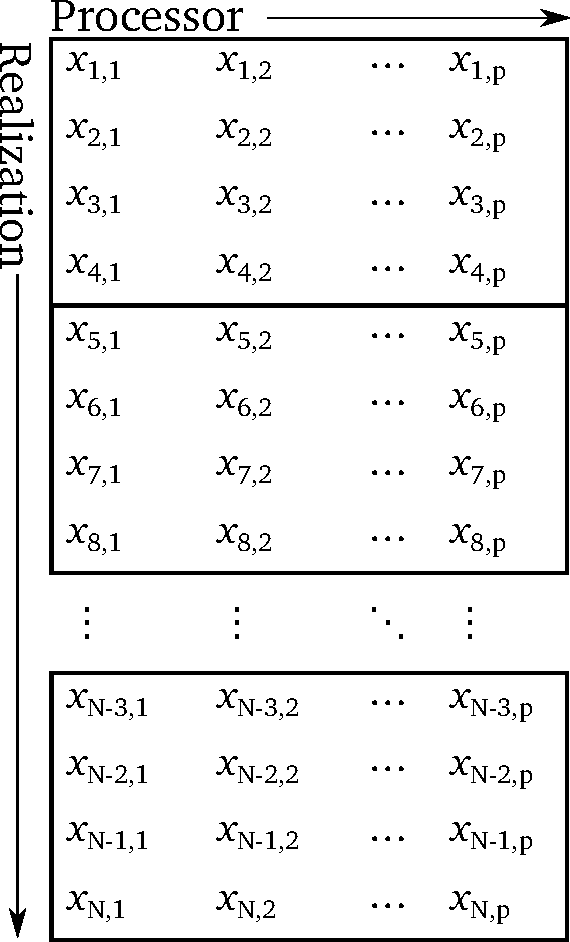
\includegraphics[width=3in]{figures/ch4/batch.pdf}
  \caption{Summation of tally scores across processors when doing statistics
    based on a single batch with $M=4$.}
  \label{fig:batch}
\end{figure}

\begin{figure}[htb]
  \centering
  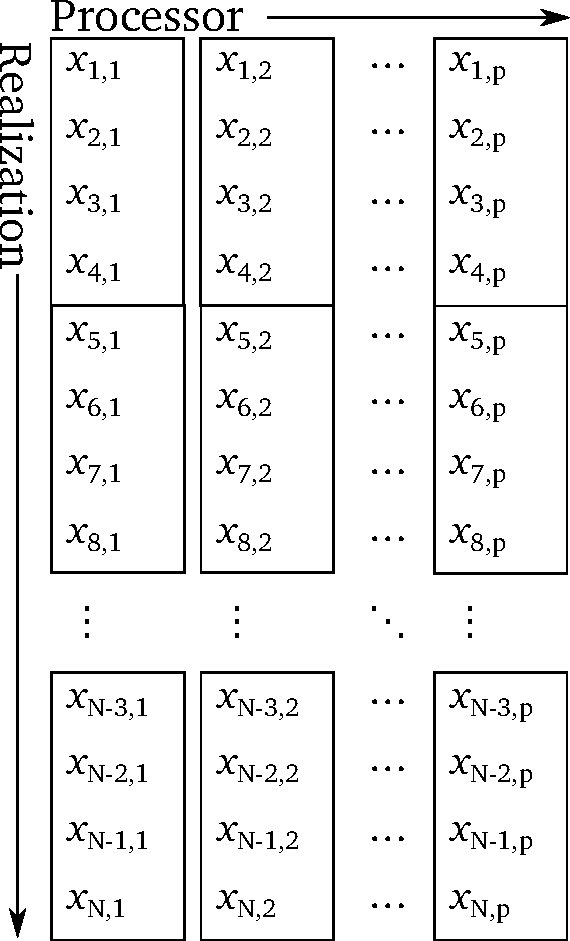
\includegraphics[width=3in]{figures/ch4/batch-parallel.pdf}
  \caption{Summation of tally scores across processors when doing statistics
    based on a batch combining realizations from a single processor with $M=4$.}
  \label{fig:batch-parallel}
\end{figure}
Rather than considering the batch to be the accumulation of scores from many
realizations across many processors, there is no reason that one cannot
reproduce the same sample mean, within floating point precision, by considering
a batch to be the accumulation of scores from many realizations on a single
processor. This idea is shown in \autoref{fig:batch-parallel}. Expressed
mathematically, our new random variable is
\begin{equation}
  z_{j,k} = \sum_{i=(j-1)M + 1}^{jM} x_{i,k}.
\end{equation}
The sample mean and its variance for this random variable would then be
\begin{align}
  \bar{z} &= \frac{1}{N'p} \sum_{j=1}^{N'} \sum_{k=1}^p z_{j,k} \\ s^2_{\bar{z}}
  &= \frac{1}{N'p-1} \left [ \frac{\sum_{j=1}^{N'} \sum_{k=1}^p z_{j,k}^2}{N'p}
    - \left ( \frac{\sum_{j=1}^{N'} \sum_{k=1}^p z_{j,k}}{N'p} \right )^2 \right
  ]
\end{align}
with $N'$ defined the same as before. In this scheme, only one reduction needs
to be performed at the very end of the simulation. The data requirement is then
$16\ell(p-1)$ bytes since we need to take the summation of the accumulated score
and accumulated squares of scores for each tally bin. Thus, the total data that
we need to communicate has been reduced by a factor of
\begin{equation}
  \frac{8\ell N(p-1)}{16\ell (p-1)} = \frac{N}{2}
\end{equation}
For large $N$, as is typical in a Monte Carlo calculation, the reduction in data
communication requirements may significantly improve the parallel efficiency.
  
%%%%%%%%%%%%%%%%%%%%%%%%%%%%%%%%%%%%%%%%%%%%%%%%%%%%%%%%%%%%%%%%%%%%%%%%%%%%%%%%
\section{Results}
\label{sec:tally-reduction-results}

To test the efficacy of the proposed method, the ability to perform statistics
based on batches, either across processors or on individual processors, was
implemented in the OpenMC Monte Carlo code. A model of the Monte Carlo
Performance Benchmark \cite{mc-hoogenboom-2011} was then simulated without (Case
1) and with (Case 2) the proposed method on a Linux cluster using eight nodes,
each with two quad-core Intel Xeon E5620 processors for a total of 64 cores. In
both cases, the neutron production rate was tallied over a 289 x 289 x 100 mesh
for a total of 8,352,100 tally bins. Each case was run with 640,000 particles
per generation with 150 inactive batches and 150 active batches\footnote{One
  generation per batch was used for both cases.}. For the neutron cross-sections
and $S(\alpha,\beta)$ tables, ENDF/B-VII.0 data was used. \autoref{tab:time}
shows the elapsed wall-clock times for these two cases.
\begin{table}[htb]
  \centering
  \caption{Elapsed wall-clock time for Monte Carlo Performance Benchmark with
    8,352,100 tally bins.}
  \label{tab:time}
  \begin{tabular}{lcc}
    \toprule
    Variable & Case 1 & Case 2 \\
    \midrule
    Total simulation time     & 1268.7 s & 953.8 s \\
    Time in inactive batches  &  425.3 s & 426.2 s \\
    Time in active batches    &  843.4 s & 527.6 s \\
    Time accumulating tallies &  348.8 s &  30.4 s \\
    \bottomrule
  \end{tabular}
\end{table}
We see that not taking the summation of the tallies across processors at every
generation results in a significant reduction in elapsed time. Most importantly,
the time spent accumulating tallies was reduced by over 90\%. The gross
reduction in simulation time will depend on many factors including simulation
parameters (e.g. how many particles are run per generation) as well as the
specific hardware for the system being used (e.g. network latency and
bandwidth).

\begin{figure}[ht]
  \centering
  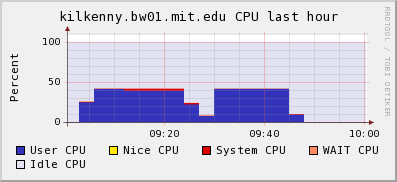
\includegraphics[width=3.5in]{figures/ch4/cpu_usage.png}
  \caption{Percentage CPU usage of entire cluster during two simulations of the
    Monte Carlo Performance Benchmark.}
  \label{fig:cpu-usage}
\end{figure}
\begin{figure}[ht]
  \centering
  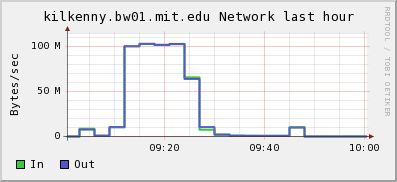
\includegraphics[width=3.5in]{figures/ch4/network.png}
  \caption{Network bandwidth during two simulations of the Monte Carlo
    Performance Benchmark.}
  \label{fig:network}
\end{figure}
\autoref{fig:cpu-usage} and \autoref{fig:network} show the CPU usage and network
communication, respectively, as reported by the Ganglia Monitoring System. On
\autoref{fig:cpu-usage}, no pause is observed between cases 1 and 2 as they were
run back-to-back. The case 2 run began at 9:29.

One can see from these figures that during the second simulation, where
reductions on tallies were not performed until the end of the simulation, the
network usage was drastically lower than when reductions were performed at every
generation. Lastly, we remark that all reported sample means of the tally
variables were identical and almost all variances were within two standard
deviations of one another.

%%%%%%%%%%%%%%%%%%%%%%%%%%%%%%%%%%%%%%%%%%%%%%%%%%%%%%%%%%%%%%%%%%%%%%%%%%%%%%%%
\section{Discussion}

A novel scheme for reducing data communication requirements in parallel Monte
Carlo calculations has been introduced here primarily aimed at criticality
calculations. In a large-scale simulation with thousands of processors, it is
natural to consider the batch to be the accumulation of scores from one
processor over the entire run ($M = N$). Provided each processor did a
sufficient amount of work to obtain reasonable statistics, the estimate of the
variance of the sample mean will be reliable since one would have $p$
realizations of the random variable.

One concern that might arise from the use of this technique is that the variance
of the sample mean will not be reproducible when running in parallel, i.e. the
variance of the sample mean will not be the same as if one had run the exact
same calculation in serial. However, the {\it expected value} of the sample
variance will be the same and the sample mean will be reproduced to within
floating point error. For users who are willing to sacrifice reproducibility of
tally variances, this detriment does not outweigh the overwhelming benefit of
drastically reduced network communication and improved parallel efficiency.

It should be noted that this method does require that the sum and sum of squares
over realizations for each tally bin be stored in memory on each
processor. Strictly speaking, the traditional methods only require storing a
temporary variable on each slave processor to accumulate scores that would be
sent to the master, i.e. the sum and sum of squares for each tally bin need to
be stored only on the master process. However, some, if not many, Monte Carlo
codes do not take advantage of this fact and simply replicate all tally data in
the memory of each process.

As a final note, even when this method is used, it may still be desirable to
perform a reduction over some global tallies such as the eigenvalue. Since the
eigenvalue is used in determining the average number of fission sites produced
at each collision, reproducibility of the sample means of local tallies can only
be preserved if the eigenvalue is the same as it would have been in a serial
run. The parallel communication necessary to perform a parallel reduction of
global tallies such as the eigenvalue will be very small since it is generally
limited to only a few quantities.

\chapter{Domain Decomposition}
\label{chap:domain-decomp}

\newcommand{\lave}{\langle \lambda \rangle}
\newcommand{\lmave}{\langle \overline{\lambda} \rangle}
\newcommand{\dpmax}{\delta{p_i^{max}}}
\newcommand{\pmax}{{p_i^{max}}}
\newcommand{\lmax}{{\lambda_i^{max}}}
\newcommand{\pbar}{\overline{P}}
\newcommand{\lbar}{\overline{\lambda}}

\section{Background}

To this point, we have described methods which will drastically improve
scalability for calculations utilizing thousands or millions of processors. With
these methods, it is possible to effectively utilize leadership class
supercomputers for Monte Carlo calculations --- but there is one caveat. The
simulations would still be forced to rely on parallelism over particles, meaning
that all problem data such as cross sections, tallies, and material compositions
must be replicated on every process. As we began discussing in
\autoref{chap:intro}, data for temperature-dependent cross sections in LWR
simulations may reach upwards of hundreds of gigabytes, and tallies can easily
exceed terabytes of memory. In order to reduce per-node memory requirements, two
strategies have been proposed: domain decomposition and data decomposition. In
this chapter, we will focus on the analysis of domain decomposition for LWR
analysis using Monte Carlo.

In many, if not most, areas of computational physics, spatial domain
decomposition is the most natural and desirable method for achieving
parallelism. Each subdomain is assigned to a different processor, and thus each
processor needs only to work on its subdomain. This makes sense when the work in
the problem is proportional to, and evenly distributed over, the size of the
problem. This is true of most mesh-based methods such as finite difference,
finite element, etc. Monte Carlo particle transport, on the other hand, does not
possess this characteristic. The computational effort in a Monte Carlo
simulation is in transporting the particles; as a result, the work is
unpredictable and not guaranteed to be evenly distributed across a
problem. Moreover, fast-streaming particles can cross the entire problem. Thus,
the use of spatial domain decomposition for Monte Carlo particle transport can
suffer from poor load balancing and overhead from network communication required
for transferring particles between subdomains.

\subsection{Review of Prior Work}

The use of domain decomposition to reduce per-node memory in Monte Carlo
particle transport simulations was first proposed by Alme et al. in 2001
\cite{js-alme-2001}. A slight variation on normal domain decomposition was also
suggested --- instead of just decomposing the geometry, subdomains could also be
replicated. The motivation for this is so that areas of the problem that have a
higher particle density, and hence more work, have proportionally more
processors dedicated to them.

Domain decomposition was subsequently implemented in a production Monte Carlo
code, Mercury, being developed by Lawrence Livermore National Laboratory
\cite{mc-procassini-2007}. A load balancing scheme similar to that proposed by
Alme et al. was also implemented in Mercury whereby the assignment of processors
to domains is periodically adjusted based on the actual work distribution
\cite{mc-procassini-2005}. The initial implementation worked only with
mesh-bashed geometries where the connectivity between regions could be readily
determined. This was later expanded to constructive solid geometries; the
algorithms used for this were described in \cite{mc-greenman-2009}.

Domain decomposition has also been applied to Monte Carlo simulation of thermal
radiation transport \cite{jcp-brunner-2006}. In that work, Brunner et
al. focused on message-passing semantics for domain decomposition schemes,
i.e. how to best communicate particles between processors. This work was later
expanded to include situations where the number of particles in a given
transport sweep was not known \emph{a priori} \cite{jcp-brunner-2009}. However,
in both of those papers, it is explicitly assumed that the problem is perfectly
load balanced, and no solutions are presented for problems that exhibit poor
load balancing.

Finally, domain decomposition is also being implemented in a new Monte Carlo
code, Shift, under development at Oak Ridge National Laboratory
\cite{physor-sly-2012}. The domain decomposition algorithm described by Brunner
\cite{jcp-brunner-2009} was chosen with the added ability to have overlapping
domains to reduce the incidence of particles crossing subdomain boundaries and
hence reduce the overall network communication.

\subsection{Recent Developments}

While the study and application of domain decomposition to Monte Carlo particle
transport simulations now has a ten year history, including the implementation
in two major Monte Carlo codes, there is surprisingly little theoretical
analysis of domain decomposition schemes. In all the papers we've reviewed thus
far \cite{js-alme-2001, mc-procassini-2005, mc-greenman-2009, jcp-brunner-2006,
  jcp-brunner-2009}, arguments about the efficacy of domain decomposition were
made based on measurements in either simple or actual codes. This is good from
the perspective that no assumptions are needed to draw conclusions; however, the
downside is that it is hard to gain an understanding of why or why not domain
decomposition would work in a given problem. In particular, the prior work does
not reveal whether domain decomposed Monte Carlo simulations could be
successfully employed for realistic LWR analysis because the test problems were
not LWR models.

Recognizing the lack of a theoretical foundation with which domain decomposition
algorithms could be analyzed, Siegel et al. published a study in 2012
\cite{jcp-siegel-2012-1} where they attempted to quantify the communication
costs in order to assess the feasibility of carrying out efficient domain
decomposition in a parameter regime relevant to LWR analysis. Key scaling
regimes were identified and performance estimates were carried out over a range
of characteristic parameters. The results demonstrated that for their chosen
model problem, good performance could be attained for reasonable effective
latency and bandwidth values with partition particle densities as low as $10^4$
per node\footnote{The testing platform in \cite{jcp-siegel-2012-1} was the Blue
  Gene/P supercomputer at Argonne National Laboratory.}. This analysis
represents an important step toward quantifying the key theoretical issues and
helped to establish the feasibility of carrying out robust LWR calculations with
Monte Carlo methods.

That being said, the analysis in \cite{jcp-siegel-2012-1} does not address the
impact of initial particle imbalances and small variations in local leakage
rates on evolving particle distributions. If particle communication costs are
potentially manageable in light of typical machine bandwidths and latencies, to
what extent will load imbalances negatively impact performance to the point
where such an approach is no longer a practical alternative? Establishing a
quantitative foundation for this performance penalty will greatly facilitate
weighing tradeoffs in deciding the best path forward among various approaches
for next-generation Monte Carlo codes. In this chapter, this issue is addressed
directly by attempting to quantify the effect of particle load imbalances on the
performance of domain decomposed Monte Carlo algorithms.

In \autoref{sec:domain-decomp-analysis}, an expression for the communication
penalty from load imbalances is derived from theoretical
considerations. However, the starting assumption is that leakage rates are
spatially constant and therefore the expression only accounts for load
imbalances due to the initial particle distribution. In a Monte Carlo
simulation, the stochastic nature of the solution will result in spatially
varying leakage rates. This is explicitly accounted for in
\autoref{sec:variable-leakage}; the resulting expression appears similar to that
derived in \autoref{sec:domain-decomp-analysis} but with an extra factor
accounting for the variable leakage rates. Finally, in
\autoref{sec:domain-decomp-evaluation}, measured data from simulations of the
Monte Carlo performance benchmark using OpenMC are used to evaluate the load
imbalance penalty for various domain sizes.

The analysis and results from this chapter are derived from a paper accepted for
publication in \emph{Journal of Computational Physics} \cite{jcp-siegel-2012-2}.

\section{Analysis}
\label{sec:domain-decomp-analysis}

\subsection{Problem definition}

To fully define the problem, let us begin with a domain $X$ segmented into $N$
non-overlapping partitions $X = \cup x_j, j=1,\dotsc,N$. In a light-water
reactor, these partitions might be chosen for convenience to be a full fuel
assembly or some part of an assembly. If we denote the initial number of
particles on partition $x_j$ as $p_{0,j}$, then the initial global particle
count $P_0$ is given by:
\begin{equation}
  \label{eq:globalP}
  P_0 = \sum_{j=1}^{N} p_{0,j}.
\end{equation}
For simplicity, assume that each partition is mapped to a single process in a
three-dimensional virtual Cartesian topology of $N$ processes. As in
\autoref{chap:fission-bank}, we are assuming a one-to-one mapping of processes
to processors, and thus we use the terms \emph{processor}, \emph{partition}, and
\emph{process} interchangeably.

On a given partition, particles local to that partition are advanced through a
sequence of interactions until they are either 1) absorbed\footnote{In a
  non-analog simulation, particles can also be killed from Russian roulette or
  other variance reduction techniques.} or 2) reach a processor boundary. For
optimal performance particles that reach the boundary are buffered locally until
all particle trajectories are computed, and are subsequently exchanged with
neighboring processors. We refer to the particle exchange phase of this process
as a \emph{stage}, and to a complete set of stages (i.e. until all particles are
absorbed) as a \emph{generation}. At the end of each generation, the fission
source is updated and the next generation begins.

Define the particle \textit{local leakage} $\lambda$ on each $x_j$ for a given
stage $i$ as
\begin{equation*}
  \lambda_{i,j} = \frac{\mbox{number of particles leaving $x_j$ at stage
      $i$}}{\mbox{number of particles starting in $x_j$ at stage $i$}}.
\end{equation*}
The goal of this analysis is to estimate the impact of initial particle load
imbalances and spatially varying local leakage values on previous performance
estimates of domain-decomposed LWR simulations.  We refer to the perfectly load
balanced, constant leakage scenario as the \emph{ideal} case. This was explored
in depth in \cite{jcp-siegel-2012-1}, where it was shown that communication
costs imposed a reasonable penalty on overall simulation time for a broad range
of relevant parameter values.

Following \cite{scott-2005} we first define the \emph{load balance} $\Gamma_i$
at each stage $i$ as
\begin{equation}
  \Gamma_i = \frac {\overline{P}_i}{p_i^{max}},
\end{equation}
where
\begin{equation*}
  \overline{P}_i = \frac{1}{N}\sum_{j=1}^{N} p_{i,j}
\end{equation*}
and $p_i^{max}$ denotes the maximum particle count on a partition at stage $i$.
The amount the load balance $\Gamma_i$ differs from the ideal case $\Gamma = 1$
measures the relative difference between the highest particle and average
particle counts:
\begin{equation}
  1- \Gamma_i = \frac{p_i^{max} - \overline{P}_i}{p_i^{max}}.
\end{equation}
Note that unlike \cite{scott-2005} we express the load imbalance in terms of
particle densities rather than execution time. Their equivalence will be argued
in the following section.

We seek to estimate a related but distinct quantity --- an upper bound for the
relative difference between the total simulation time per generation of the
non-ideal case and the ideal case. We define this relative difference as the
\textit{load imbalance penalty} $\Delta$:
\begin{equation}
  \label{eq:load-imbalance}
  \Delta = \frac{\tau' - \tau}{\tau} = \frac{\tau'}{\tau} - 1,
\end{equation}
where $\tau$ denotes the total simulation time per generation in the ideal case,
and $\tau'$ for the non-ideal case.  Note that an expression for $\Delta$ must
include both the particle tracking as well as the communication costs across all
stages of a given generation. While related to the per-stage particle load
balance, the load imbalance penalty is a distinct quantity.

\subsection{Basic properties}

Given this simple problem definition above, and assuming that leakage at the
problem boundary is negligible (a good approximation for power reactors), the
\emph{global} number of particles at any \emph{stage} is given by
\begin{equation}
  \label{eq:pg}
  P_{i+1} = \sum_{j=1}^N p_{i+1,j} = \sum_{j=1}^N \lambda_{i,j}
  p_{i,j} \hspace{.5in} i=0,1,\dotsc,M-1
\end{equation}
where $M$ denotes the final stage in the generation --- i.e. when all particles
are absorbed and none remain. We emphasize again that $P_i$ denotes the global
particle count at stage $i$ while $p_{i,j}$ denotes the local particle count on
partition $j$ at stage $i$.

To estimate $\tau'$, the per-generation simulation time in the non-ideal case,
we seek an expression for the \emph{local} particle distribution --- i.e. the
number of particles on each partition $x_j$ at stage $i$. Assuming the leakage
is equal on all surfaces, the neutron count on a partition is given by:
\begin{equation}
  \label{eq:pl}
  p_{i+1,j} = \frac{1}{6} \left( \lambda_{i,j1}p_{i,j1} + \lambda_{i,j2}p_{i,j2}
  + \dotsb + \lambda_{i,j6}p_{i,j6} \right)
\end{equation}
where $j1,j2,\dotsc,j6$ denote the six immediate neighbors of partition $j$ on a
Cartesian lattice. Equation \eqref{eq:pl} simply states that, in advancing
stages, a given partition receives 1/6th of the leaked particles from each of
its six neighbors on a Cartesian grid.

Equation \eqref{eq:pl} shows that the evolution of the local particle
distribution depends on the detailed alignment of the local particle counts and
the local leakage rates. To reduce it further requires additional
assumptions. We start by noting that, in an LWR, the neutron spectrum and
material heterogeneities are roughly constant from partition to partition (this
property is demonstrated using simulation data in
\autoref{sec:domain-decomp-evaluation}). This observation makes the case of
approximately spatially uniform local leakages of great practical interest in
the present context, and thus we initially consider the case of $\lambda_{i,j} =
\lambda_i$. Note that we still expect non-trivial per-stage variation in
leakages as neutron energies will shift toward the thermal range with increasing
stages. Important model corrections for small spatial variations in $\lambda$
will be considered in \autoref{sec:variable-leakage}.

For spatially constant $\lambda$, \eqref{eq:pg} then becomes
\begin{align}
  \label{eq:pg2}
  P_{i} &= \sum_{j=1}^N \lambda_{i-1} p_{i-1,j} = \lambda_{i-1}
  \sum_{j=1}^Np_{i-1,j} = \lambda_{i-1} P_{i-1} \nonumber \\
  &= \lambda_{i-1} \lambda_{i-2} \dotsm \lambda_{0} P_0 \nonumber \\
  &\approx {\lave}^{i} P_0 \hspace{2in} i=1,2,\dotsc,M
\end{align}
where $\lave$ is defined as the geometric mean of the leakage rate,
\begin{equation}
  \label{eq:cycle_mean}
  \lave = \sqrt[M]{\lambda_{M-1}\lambda_{M-2} \dotsm \lambda_{0} }.
\end{equation}
Equation \eqref{eq:pl} then simplifies to
\begin{equation}
  \label{eq:meanp}
  p_{i+i,j} = \frac{\lambda_i}{6} \left( p_{i,j1} + p_{i,j2} + \cdots + p_{i,j6}
  \right)
\end{equation}
Equation \eqref{eq:meanp} shows that, for spatially constant $\lambda$, at each
subsequent stage each partition has the average value of the total leaked
particles from the neighboring partitions in the previous stage.  Equation
\eqref{eq:pg2} shows that, in the case of constant $\lambda$, the particle load
imbalance does not affect the number of stages required to complete a
generation, which can be estimated by setting $P_i = 1$ in \eqref{eq:pg2}:
\begin{equation}
  \label{eq:kfinal}
  {\lave}^M P_0 = 1 \implies M \approx -\frac{\log P_0}{\log \lave}.
\end{equation}
Both properties are used in the analysis that follows.

\subsection{Expression for \texorpdfstring{$\tau$}{tau}}

Given these basic properties, we first seek an estimate of the total
per-generation cost in the idealized case of an initial even distribution of
particles and spatially constant $\lambda$.  This is accomplished by decomposing
$\tau$ into a local work $\tau_l$ and inter-process communication $\tau_c$
component as
\begin{equation}
  \tau = \tau_l + \tau_c.
\end{equation}
In the case of perfect load balancing and assuming a roughly equal distribution
of track length and neutron spectra across partitions (i.e. our earlier
assumption of constant $\lambda$), the local work $\tau_l$ should be roughly
proportional to the total number of particles tracked on a partition in a given
generation,
\begin{equation}
  \label{eq:loc_work}
  \tau_{l} \approx \mu \sum_{i=0}^{M} \overline{P}_{i},
\end{equation}
where the constant $\mu$ is a measure of the tracking time per particle, and
where it is understood that the particle count $p_{i,j}$ is the same on any
given partition, since all partitions are equivalent in the ideal case.

The communication time $\tau_c$ can be further decomposed into a latency and
bandwidth component \cite{jcp-siegel-2012-1}. For each generation, a total of
$M$ messages need to be sent to each processor's six neighbors, so in general
the total time per generation due to message latency can be modeled as
proportional to $6 \alpha M$, where $\alpha$ is some measure of the effective
application-level latency for a single send.

If we ignore the dependence of $\lambda$ on stage, by definition $\lambda
\overline{P}_i$ particles are sent from each processor at stage $i$, and the
total number of particles sent in a generation from any processor is $\lambda
\sum_i \overline{P}_i$. Thus, the bandwidth term can be roughly modeled as
$\beta \lambda \sum_i \overline{P}_i$, where $\beta$ denotes the effective
inverse bandwidth for nearest-neighbor exchanges (expressed in time per
particle).

When we account for stage dependence $\lambda$ is replaced by $||\lambda||$,
defined as the solution to the $M$th order polynomial:
\begin{equation}
  \label{eq:lmean}
  \sum_{i=1}^M ||\lambda||^i = \lambda_0 + \lambda_1\lambda_0 + \cdots +
  \lambda_{M-1}\lambda_{M-2}\dotsm\lambda_0.
\end{equation}
The bandwidth term can then be written as:
\begin{align}
  \beta \sum_{i=0}^{M-1} \lambda_i \overline{P}_i &= \beta(\lambda_0
  \overline{P}_0 + \lambda_1 \overline{P}_1 + \dotsb +
  \lambda_{M-1}\overline{P}_{M-1}) \nonumber \\
  &= \beta(\lambda_0 \pbar_0 + \lambda_1 \lambda_0 \pbar_0 + \dotsb +
  \lambda_{M-1}\lambda_{M-2}\dotsm\lambda_0 \pbar_0) \nonumber \\
  &=\beta\pbar_0(\lambda_0 + \lambda_1\lambda_0 + \dotsb +
  \lambda_{M-1}\lambda_{M-2}\dotsm\lambda_0) \nonumber \\
  &= \beta\pbar_0\sum_{i=1}^M ||\lambda||^i.
\end{align}
Using these relations together with \eqref{eq:kfinal} then yields the following
expression for the total communication time:
\begin{equation}
  \label{eq:tot_comm}
  \tau_c = -6 \alpha \frac{\log P_0}{\log \lave} + \beta\pbar_0\sum_{i=1}^M
  ||\lambda||^i.
\end{equation}
Using the same approach on \eqref{eq:loc_work} and combining with
\eqref{eq:tot_comm} gives the final expression for total simulation time in the
idealized case:
\begin{align}
  \label{eq:tau1}
  \tau &= -6 \alpha \frac{\log P_0}{\log \lave} + \mu \pbar_0 \sum_{i=0}^M
  ||\lambda||^i + \beta\pbar_0\sum_{i=1}^M ||\lambda||^i \nonumber \\
  &= -6 \alpha \frac{\log P_0}{\log \lave} + \left ( \mu \sum_{i=0}^M
  ||\lambda||^i + \beta\sum_{i=1}^M ||\lambda||^i \right ) \pbar_0.
\end{align}

\subsection{Expression for \texorpdfstring{$\tau'$}{tau'}}

We now seek an estimate for the total simulation time $\tau'$ in the presence of
an initial load imbalance. For convenience we first express $p_{i,j}$ as a
combination of partition mean and fluctuating parts. That is,
\begin{equation}
  \label{eq:mean}
  \delta p_{i,j} = p_{i,j} - \overline{P}_i.
\end{equation}
When a load imbalance is present the partition with the largest particle count
controls the total performance cost. If we denote the particle count on this
process as $p^{max}_i = \overline{P}_i + \dpmax$, then by the same logic as in
the previous section, the load-imbalanced performance is:
\begin{equation}
  \label{eq:tauprime-1}
  \tau' = -6 \alpha \frac{\log P_0}{\log \lave} + \mu \sum_{i=0}^M p_i^{max} +
  \beta \sum_{i=0}^{M-1} \lambda_i p_i^{max}.
\end{equation}
While we cannot directly evaluate the sum of $p_i^{max}$, a simple upper bound
can be derived by recognizing that, assuming roughly equal leakage to each
neighbor, the largest possible value of $p$ at stage $i+1$ occurs if all six
neighbors of a partition contain $p_i^{max}$ particles. Thus,
\begin{equation}
  \label{eq:pmax-ub1}
  p^{max}_{i+1} \le \lambda_i p^{max}_i.
\end{equation}
This implies that
\begin{align}
  \label{eq:pmax-expand1}
  \sum_{i=0}^M p_i^{max} &\le \mu \left ( p_0^{max} + \lambda_0 p_0^{max} +
  \lambda_1 \lambda_0 p_0^{max} + \dotsb + \lambda_{M-1} \lambda_{M-2} \dotsm
  \lambda_0 p_0^{max} \right ) \nonumber \\
  &= \mu p_0^{max} \left ( 1 + \lambda_0 + \lambda_1 \lambda_0 + \dotsb +
  \lambda_{M-1} \lambda_{M-2} \dotsm \lambda_0 \right ) \nonumber \\
  &= \mu p_0^{max} \sum_{i=0}^M ||\lambda||^i
\end{align}
and
\begin{align}
  \label{eq:pmax-expand2}
  \sum_{i=0}^{M-1} \lambda_i p_i^{max} &\le \mu \left ( \lambda_0 p_0^{max} +
  \lambda_1 p_1^{max} + \dotsb + \lambda_{M-1} p_{M-1}^{max} \right ) \nonumber \\
  &= \mu \left ( \lambda_0 p_0^{max} + \lambda_1 \lambda_0 p_0^{max} + \dotsb +
  \lambda_{M-1} \lambda_{M-2} \dotsm \lambda_0 p_0^{max} \right ) \nonumber \\
  &= \mu p_0^{max} \left ( \lambda_0 + \lambda_1 \lambda_0 + \dotsb +
  \lambda_{M-1} \lambda_{M-2} \dotsm \lambda_0 \right ) \nonumber \\
  &= \mu p_0^{max} \sum_{i=1}^M ||\lambda||^i.
\end{align}
Substituting \eqref{eq:pmax-expand1} and \eqref{eq:pmax-expand2} into
\eqref{eq:tauprime-1}, we obtain
\begin{align}
  \label{eq:tauprime-2}
  \tau' &= -6 \alpha \frac{\log P_0}{\log \lave} + \mu p_0^{max} \sum_{i=0}^M
  ||\lambda||^i + \beta p_0^{max} \sum_{i=1}^M ||\lambda||^i \nonumber \\
  &= -6 \alpha \frac{\log P_0}{\log \lave} + \left( \mu \sum_{i=0}^M
  ||\lambda||^i + \beta \sum_{i=1}^M ||\lambda||^i \right ) p_0^{max}.
\end{align}
With expressions for $\tau$ and $\tau'$, we can now proceed to estimate the load
imbalance penalty.

\subsection{Expression for \texorpdfstring{$\Delta$}{Delta}}

Using \eqref{eq:load-imbalance}, \eqref{eq:tau1}, and \eqref{eq:tauprime-2} and
noting that $p_0^{max} = \pbar_0 + \delta p_0^{max}$, we get the following
expression for $\Delta$:
\begin{equation}
  \label{eq:delta1}
  \Delta = \frac{\displaystyle \left( \mu \sum_{i=0}^M ||\lambda||^i + \beta
    \sum_{i=1}^M ||\lambda||^i \right ) \delta p_0^{max}}{\displaystyle -6
    \alpha \frac{\log P_0}{\log \lave} + \left ( \mu \sum_{i=0}^M ||\lambda||^i
    + \beta\sum_{i=1}^M ||\lambda||^i \right ) \pbar_0}.
\end{equation}
We can simplify \eqref{eq:delta1} slightly by dividing each term by the
expression in parentheses, i.e.
\begin{equation}
  \label{eq:delta2}
  \Delta = \frac{\delta p_0^{max}}{\displaystyle -6 \alpha \frac{\log P_0}{\log
        \lave} \left( \mu \sum_{i=0}^M ||\lambda||^i + \beta \sum_{i=1}^M
      ||\lambda||^i \right )^{-1} + \pbar_0}.
\end{equation}
The first term in the denominator of \eqref{eq:delta2} measures the importance
of latency relative to bandwidth and tracking timescales, which is presumed to
be small for typical problem sizes and parameter regimes (e.g. see
\cite{jcp-siegel-2012-1}) but which is retained here for the sake of generality.
Note that \eqref{eq:delta2} implies that
\begin{equation}
  \label{eq:delta3}
  \Delta \le \frac{\delta p_0^{max}}{\overline{P_0}} = \frac{1}{\Gamma_0} - 1,
\end{equation}
which should be a good approximation for applications where the latency term is
much smaller than the bandwidth and tracking terms. We see, then, that assuming
spatially constant $\lambda$ and given isotropic neutron local leakage and
constant mean tracking rates per partition, we can establish an upper bound for
$\Delta$ entirely in terms of the initial particle configuration.

\section{Variable leakage rates}
\label{sec:variable-leakage}

Equation \eqref{eq:delta2} should give a reasonable estimate for reactor
applications across a range of parameter values, where material inhomogeneities
are roughly equally distributed and thus local leakage rates show very little
variation. However, it fails to capture a critical effect that emerges as we
move to smaller partition sizes, and which sets an important limit on the
utility of the domain-decomposed approach. To see this we explicitly account for
spatially variant, non-constant leakage in the formulation of the model.

Consider a distribution of leakage rates across partitions at a given stage with
a maximum value defined as:
\begin{equation}
  \lambda^{max}_i = \max \left\{\lambda_{i,j} : 1 \le j \le N\right\}.
\end{equation}
In estimating the computation time for this scenario compared to the ideal case
(i.e. calculating $\Delta$), the question arises of what corresponding spatially
constant value of $\lambda$ should be used for the ideal case. Several options
are reasonable, but here we choose a mean value that preserves
stages. Specifically, if we define a particle-weighted mean leakage as:
\begin{equation}
  \label{eq:pmean}
  \lbar_i = \frac{\sum_{j=1}^{N} p_{i,j} \lambda_{i,j}}{P_i}
\end{equation}
then the ideal and non-ideal cases are guaranteed to have the same number of
global particles at successive stages:
\begin{equation*}
  \frac{P_{i+1}}{P_i} = \frac{1}{P_i}\sum_{j=1}^N \lambda_{i,j} p_{i,j} =
  \lbar_i.
\end{equation*}
Thus, the performance for the ideal case with variable leakage rates is now
\begin{align}
  \label{eq:tau2}
  \tau &= -6 \alpha \frac{\log P_0}{\log \lmave} + \mu \sum_{i=0}^M
  \overline{P}_i + \beta \sum_{i=0}^{M-1} \lbar_i \overline{P}_i
  \nonumber \\ &= -6 \alpha \frac{\log P_0}{\log \lmave} + \left ( \mu
  \sum_{i=0}^M ||\lbar||^i + \beta\sum_{i=1}^M
  ||\lbar||^i \right ) \pbar_0
\end{align}
where $\lmave$ is the geometric mean (over stages) of the particle-weighted mean
leakage at each stage, i.e.
\begin{equation*}
    \lmave = \sqrt[M]{\lbar_{M-1}\lbar_{M-2} \dotsm
      \lbar_{0}}.
\end{equation*}
and $||\lbar||$ is defined analogous to \eqref{eq:lmean}:
\begin{equation*}
  \sum_{i=1}^M ||\lbar||^i = \lbar_0 + \lbar_1 \lbar_0 + \dotsb + \lbar_{M-1}
  \lbar_{M-2} \dotsm \lbar_0.
\end{equation*}
Following \eqref{eq:pmax-ub1}, then, the largest possible particle count at
stage $i$ occurs on partition $x_j$ if on its six neighbors $\pmax$ coincides
with $\lmax$. That is,
\begin{equation}
  \label{eq:ub2}
  p_{i+1}^{max} \le \lmax p_i^{max}.
\end{equation}
This implies that
\begin{equation}
  \tau' \le -6\alpha\frac{\log P_0}{\log \lmave} + \mu \sum_{i=0}^M \pmax
  \nonumber + \beta \sum_{i=0}^{M} \lmax \pmax.
\end{equation}
Following the same logic as in \eqref{eq:pmax-expand1}, \eqref{eq:pmax-expand2},
and \eqref{eq:tauprime-2} we can derive an upper bound for $\tau'$ in the case
of variable $\lambda$:
\begin{equation}
  \label{eq:tauprime-3}
  \tau' \le -6 \alpha \frac{\log P_0}{\log \lmave} + \left( \mu \sum_{i=0}^M
  ||\lambda^{max}||^i + \beta \sum_{i=1}^M ||\lambda^{max}||^i \right )
  p_0^{max}
\end{equation}
where $||\lambda^{max}||$ is defined as
\begin{equation*}
  \sum_{i=1}^M ||\lambda^{max}||^i = \lambda^{max}_0 + \lambda^{max}_1
  \lambda^{max}_0 + \dotsb + \lambda^{max}_{M-1} \lambda^{max}_{M-2} \dotsm
  \lambda^{max}_0.
\end{equation*}
We can then use \eqref{eq:tau2} and \eqref{eq:tauprime-3} to obtain the
following upper bound for the load imbalance:
\begin{equation}
  \label{eq:delta4}
  \Delta \le \frac{\displaystyle -6 \alpha \frac{\log P_0}{\log \lmave} + \left(
    \mu \sum_{i=0}^M ||\lambda^{max}||^i + \beta \sum_{i=1}^M
    ||\lambda^{max}||^i \right ) p_0^{max}}{\displaystyle -6 \alpha \frac{\log
      P_0}{\log \lmave} + \left ( \mu \sum_{i=0}^M ||\lbar||^i +
    \beta\sum_{i=1}^M ||\lbar||^i \right ) \pbar_0} - 1.
\end{equation}
Again, taking the very reasonable assumption (see e.g. \cite{jcp-siegel-2012-1})
that the latency term is small relative to the sum of the bandwidth and tracking
terms, we can establish a more intuitive upper bound:
\begin{equation}
  \label{eq:delta5}
  \Delta \le \frac{C}{\Gamma_0} - 1.
\end{equation}
where we have defined the factor $C$ as
\begin{equation}
  \label{eq:correction1}
  C = \frac{\displaystyle \mu \sum_{i=0}^M ||\lambda^{max}||^i + \beta
    \sum_{i=1}^M ||\lambda^{max}||^i}{\displaystyle \mu \sum_{i=0}^M ||\lbar||^i
    + \beta\sum_{i=1}^M ||\lbar||^i}.
\end{equation}
One can interpret this as follows --- accounting for variable leakage rates has
introduced a ``correction factor'' relative to \eqref{eq:delta3}; clearly, when
$||\lbar|| = ||\lambda^{max}||$, \eqref{eq:delta5} reduces to
\eqref{eq:delta3}. Further simplification can be made to \eqref{eq:correction1}
by writing
\begin{equation}
  \label{eq:correction2}
  C = \frac{\displaystyle \mu + \beta \frac{\sum_{i=1}^M
      ||\lambda^{max}||^i}{\sum_{i=0}^M ||\lambda^{max}||^i}}{\displaystyle \mu
    + \beta \frac{\sum_{i=1}^M ||\lbar||^i}{\sum_{i=0}^M ||\lbar||^i}}
  \frac{\sum_{i=0}^M ||\lambda^{max}||^i}{\sum_{i=0}^M ||\lbar||^i}
\end{equation}
and subsequently using the approximation
\begin{equation}
  \label{eq:sum-approx}
  \sum_{i=1}^M x^i \approx x \sum_{i=0}^M x_i
\end{equation}
which should hold for large $M$. Applying \eqref{eq:sum-approx} to
$||\lambda^{max}||$ and $||\lbar||$ in \eqref{eq:correction2} yields
\begin{equation}
  \label{eq:correction3}
  C \approx \frac{\mu + \beta ||\lambda^{max}||}{\mu + \beta ||\lbar||}
  \frac{\sum_{i=0}^M ||\lambda^{max}||^i}{\sum_{i=0}^M ||\lbar||^i}.
\end{equation}
The greater the spatial variation in leakage rates the more the system bandwidth
and neutron tracking rates factor into the performance. The implications of
these formulas are explained in the simple tests below, where we aim to estimate
$C$ as a function of the main problem parameters.

\section{Evaluation of model}
\label{sec:domain-decomp-evaluation}

For a given initial particle configuration, evaluation of the model equation
\eqref{eq:delta4} requires estimates for the particle tracking rate $\mu$, the
application-level inverse bandwidth $\beta$ and latency $\alpha$, and the local
leakage rate estimates from which to compute $||\lambda^{max}||$ and
$||\lbar||$. These parameters vary widely by both machine and specific code
application. Here we evaluate these terms in a parameter regime relevant to LWR
physics on modern supercomputers. Other applications and machine architectures
can be evaluated with appropriate values of these parameters.

\subsection{Leakage rates}

While best-estimate application-level bandwidth and latency terms can be
estimated from standard benchmarks (e.g. \cite{cpe-wallcraft-2000}), the leakage
rate terms in \eqref{eq:delta4} are more difficult to approximate. Simplified
models, such as the Wigner rational approximation \cite{ae-pashkin-1970} provide
rough estimates of expected domain-dependent leakage rates, but do a poor job at
estimating stage dependence. Thus, to be as precise as possible we measure these
values directly using an existing Monte Carlo particle transport code --- OpenMC
\cite{ane-romano-2013}. Note that, though parallel, OpenMC does not employ
domain decomposition. To model partitions and stages, we overlay within OpenMC
an imaginary grid decomposition and effectively measure the behavior of
particles between fictional stages during a generation. The resulting particle
loads and number of stages should be identical to a truly domain decomposed code
using an identical computational grid.

The specific test executed was based on the Monte Carlo Performance benchmark
\cite{mc-hoogenboom-2011} using $0.5$ billion active particle histories.
Leakage rates at each stage and within each partition were measured for three
cases: a single assembly, quarter-assembly, and ninth-assembly partition overlay
using 20, 40, and 60 axial levels, respectively. In each case, the benchmark
model was simulated on a 19-node Intel Xeon dual core cluster with 1 million
neutrons per generation for 150 inactive and 500 active generations. For neutron
cross sections, data from ENDF/B-VII.0 was used.

\autoref{fig:leakage-maps} illustrates the scale and level of variation in local
leakage rates for the full, quarter, and one-ninth assembly cases.  The plots
shown are for the axial level nearest the middle of the core at stage zero. They
represent ``typical'' leakage rate distributions and are intended to graphically
illustrate their relative lack of spatial coherency and small range of
values. Also, it is evident from the figure that, as expected, leakage rates
increase non-trivially with decreasing partition size.
\begin{figure}[ht!]
  \centering
  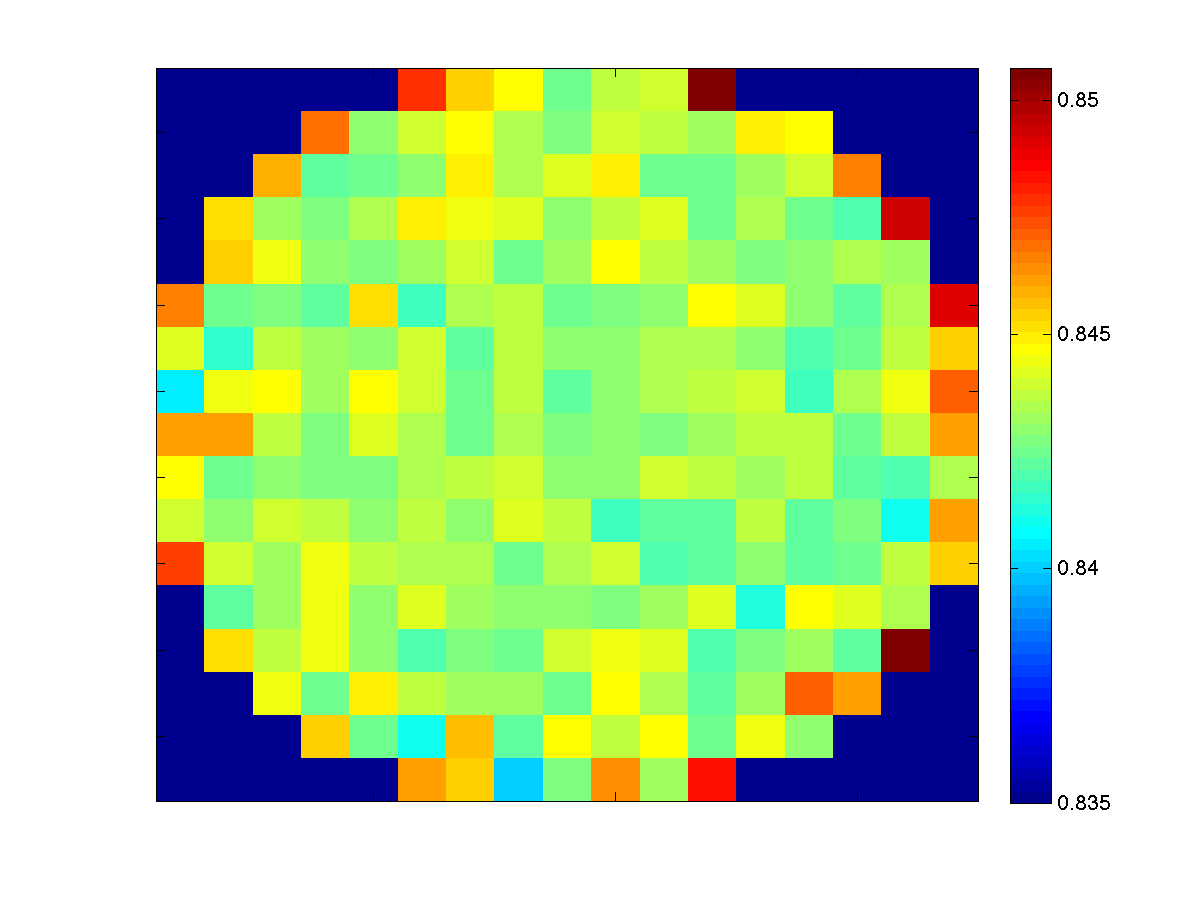
\includegraphics[width=2.5in]{figures/ch5/leakage_map1.png}
  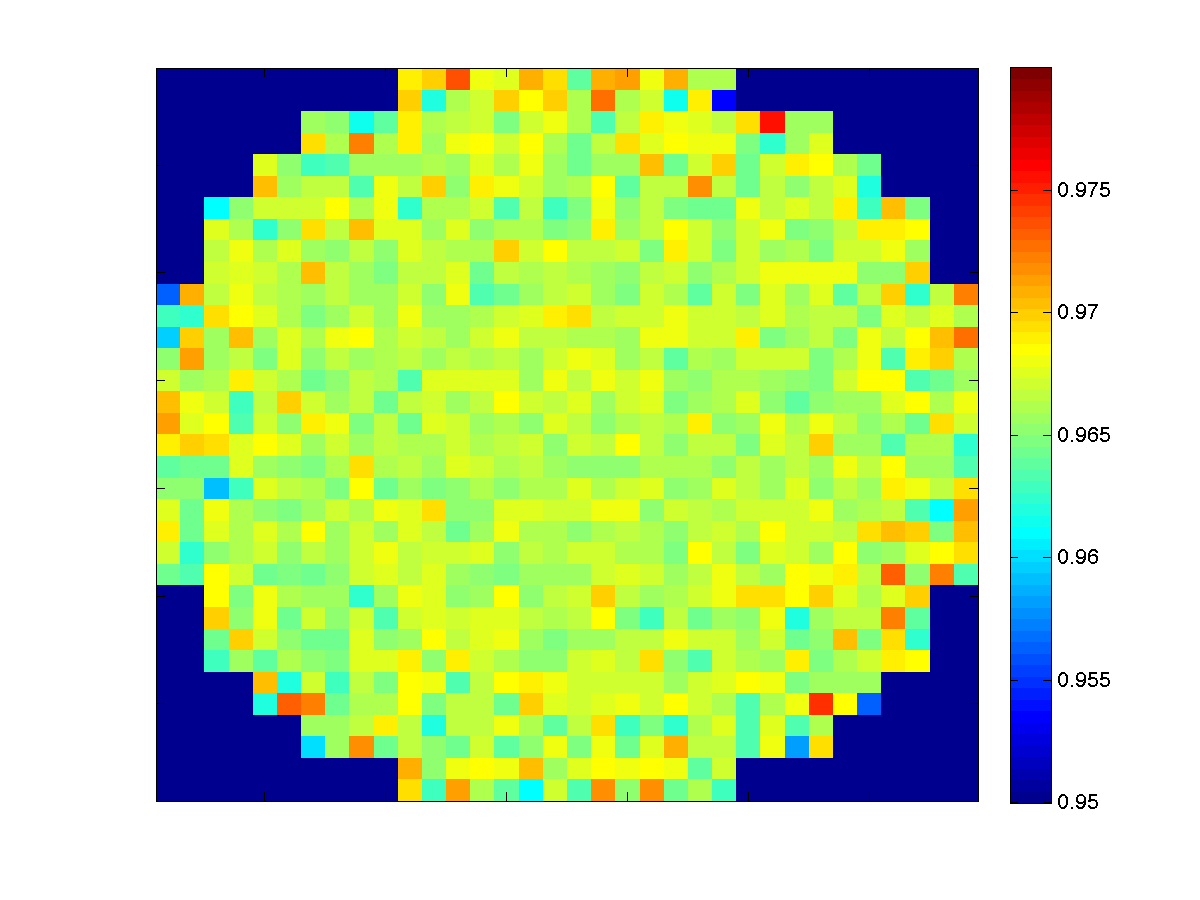
\includegraphics[width=2.5in]{figures/ch5/leakage_map1_4.png}
  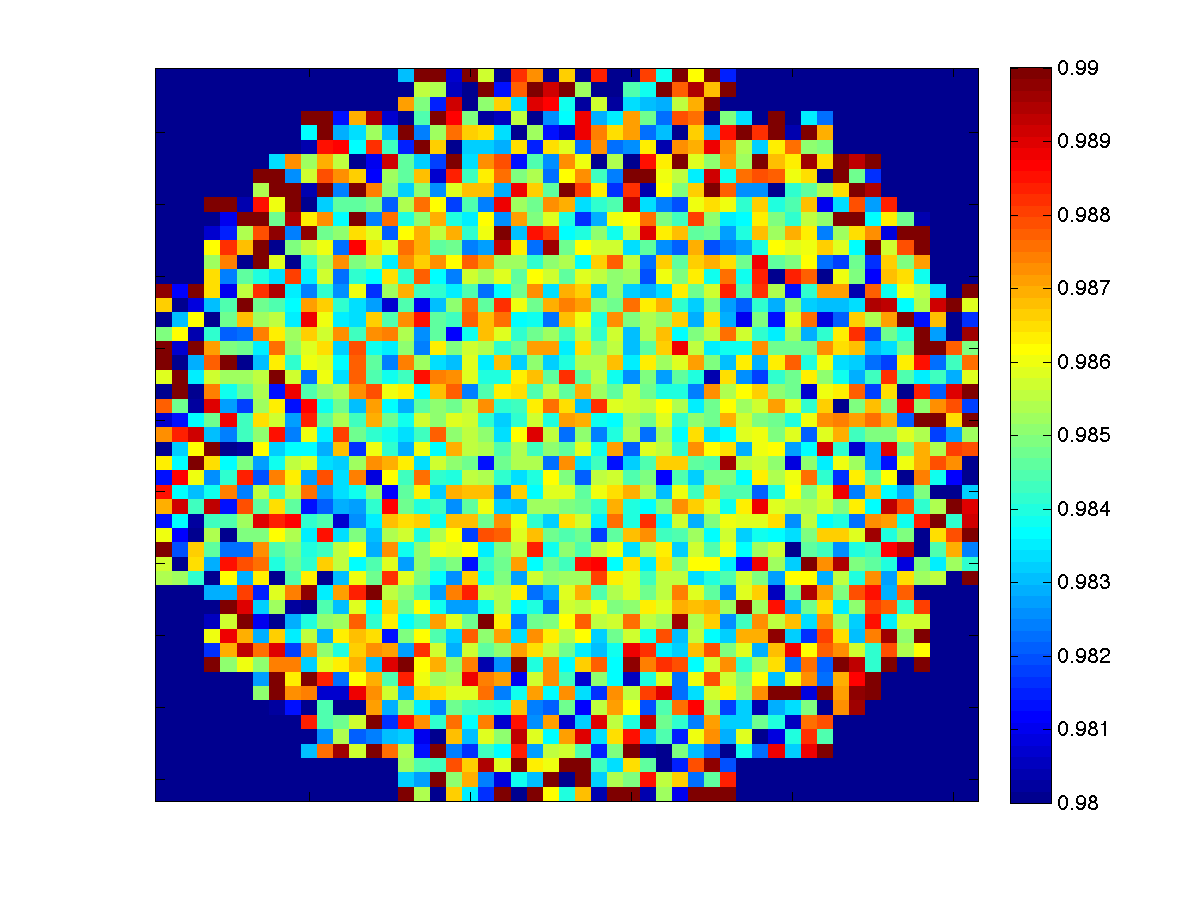
\includegraphics[width=2.5in]{figures/ch5/leakage_map1_9.png}
  \caption{Leakage rate distributions for the full, quarter, and ninth assembly
    experiments.}
  \label{fig:leakage-maps}
\end{figure}
To see this more clearly, \autoref{fig:avg-leakage} shows the stage-dependent
mean and standard deviation (error bar overlay) of $\lambda$ for each
simulation.  In each case, we see the clear trend that as neutrons thermalize
(undergo successive collisions), the leakage rates decrease corresponding to a
shorter mean free path. Furthermore, the superposed standard deviations indicate
extremely small spatial variation in the first several stages, which accounts
for the majority of data movement and performance cost. When particle counts are
small in later stages statistical variations result in larger standard deviation
values, but their impact on total performance is expected to be small. We note
that this very small spatial variation hints that the correction factor for
variable $\lambda$ in \eqref{eq:correction1} may be small. This is evaluated in
the next section.
\begin{figure}[ht!]
  \centering
  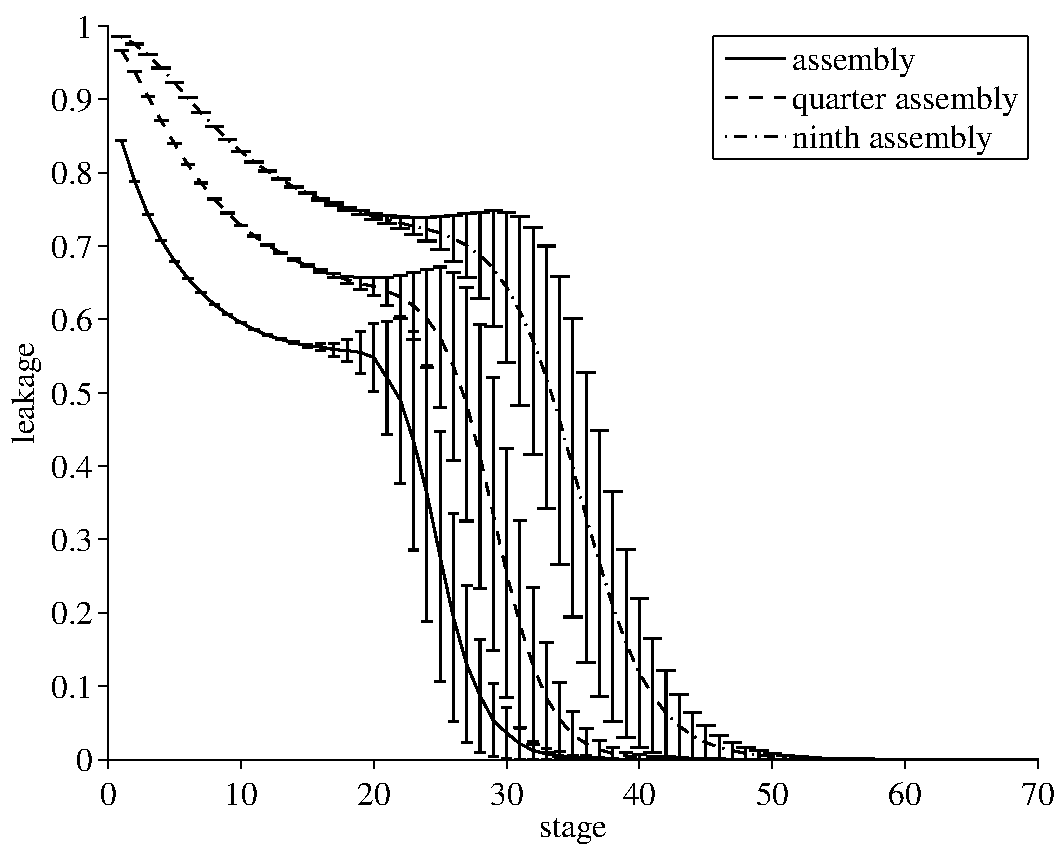
\includegraphics[width=4.0in]{figures/ch5/avg_leakage.pdf}
  \caption{Average values of leakage rate $\lambda$ at each stage for the full,
    quarter, and ninth assembly experiments.}
  \label{fig:avg-leakage}
\end{figure}

We next test the predictions for total number of stages $M$ per generation given
by \eqref{eq:kfinal}, i.e.
\begin{equation}
  \label{eq:totalstages}
  M = -\frac{\log P_0}{\log \lmave}.
\end{equation}
The values of the $\lmave$ were calculated for each of the three experiments and
inserted into \eqref{eq:totalstages}. \autoref{tab:num-stages} compares these
results with those obtained directly from the simulation. The model formula
behaves as expected, differing by only several percent from the measured
data. Exact correspondence is not expected --- statistical fluctuations, slight
anisotropies and other minor effects are likely to yield small variations. For
practical purposes though the current estimate is more than adequate.
\begin{table}[htb]
  \centering
  \begin{tabular}{c c c}
    \toprule
    Experiment & $M$ (data) & $M$ (model)  \\
    \midrule
    Full assembly & $41$ & $39$  \\
    Quarter assembly & $52$ & $51$ \\
    Ninth assembly & $71$ & $70$  \\
    \bottomrule
  \end{tabular}
  \caption{The number of stages $M$ for the three numerical experiments vs. the
    value predicted by \eqref{eq:totalstages}.}
  \label{tab:num-stages}
\end{table}

It is furthermore instructive to test the fidelity of \eqref{eq:ub2} to the true
measure maximum particle counts at each stage. While \eqref{eq:ub2} is a true
statement, in a practical sense it is of questionable value if it over-predicts
$p^{max}_i$ by too significant a margin. \autoref{fig:ub-source} shows the
computed value of $p^{max}_i$ for each stage versus the value predicted by
\eqref{eq:ub2}. Given that leakage rate variation is very small spatially, it is
not surprising to see that \eqref{eq:ub2} works extremely well as an upper
bound, over-predicting the measured value by less than $1.0\%$ for the initial
stages (which account for the bulk of the particle transfers).
\begin{figure}[ht!]
  \centering
  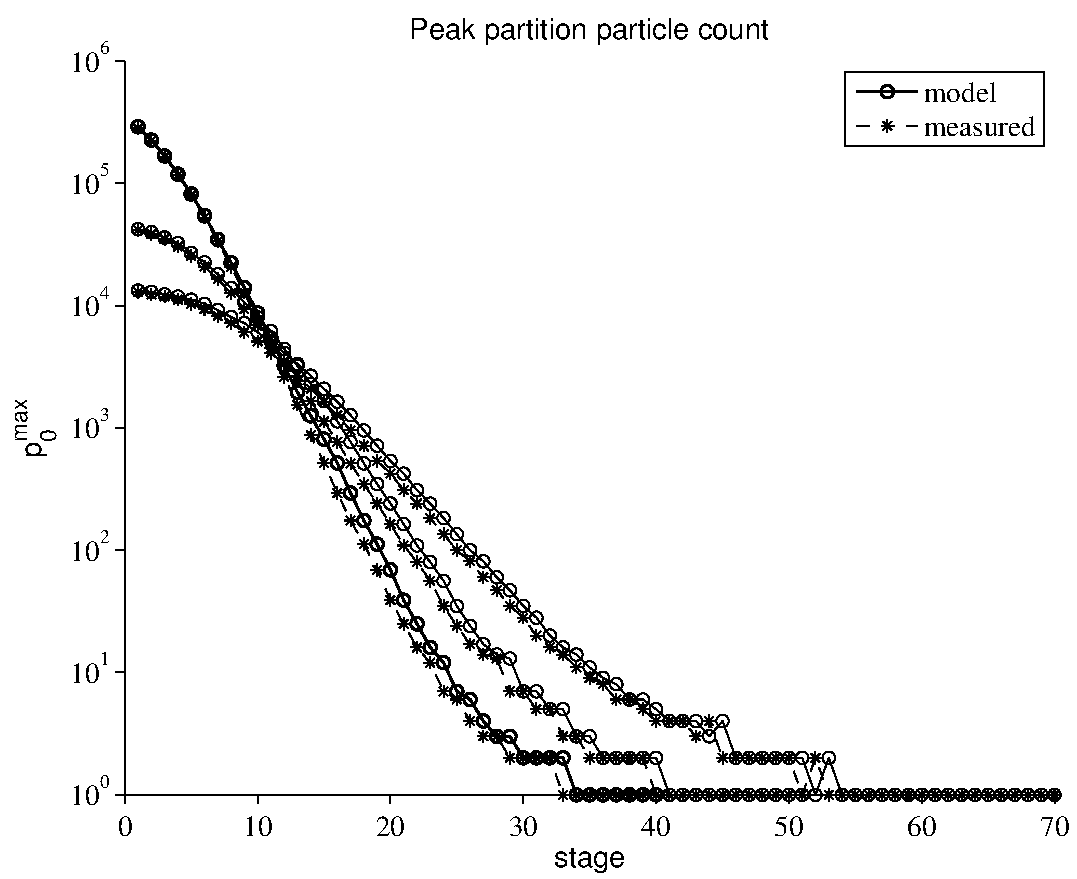
\includegraphics[width=4.0in]{figures/ch5/ub_source.pdf}
  \caption{Computed values of $p^{max}$ for each stage versus the value
    predicted by \eqref{eq:ub2}.}
  \label{fig:ub-source}
\end{figure}

\subsection{Evaluation of correction factor $C$ and penalty \texorpdfstring{$\Delta$}{Delta}}

Given an initial particle configuration and reasonable estimates for leakage, it
remains to evaluate $C$ in \eqref{eq:correction1}. To reiterate, under the
assumption of spatially constant leakage $C$ is unity and the load imbalance
penalty can be upper bounded by the initial particle configuration as
$\frac{p_0^{max}}{\overline{P_0}}$. When leakage rates vary spatially $C$
measures the amplification of the performance penalty. We estimate $C$ in two
steps, first evaluating the contribution of the bandwidth and tracking times,
given by the first term in \eqref{eq:correction3}:
\begin{equation}
  \label{eq:C-factor-ratio}
  \frac{\mu + \beta ||\lambda^{max}||}{\mu + \beta ||\lbar||} = \frac{1 +
    \frac{\beta}{\mu}||\lambda^{max}||}{1 + \frac{\beta}{\mu}||\lbar||}.
\end{equation}
Note that for any conventional machine $\beta \ll \mu$, reflecting that tracking
rates are much slower than inter-processor communication, and since $||\lbar||
\sim ||\lambda^{max}||$, \eqref{eq:C-factor-ratio} remains very close to unity
and contributes negligibly to the overall load imbalance. This demonstrates the
important fact that for all practical purposes the system bandwidth and latency
have very little effect on the load imbalance penalty, which is determined
almost entirely by the physics of neutron transport as expressed by the local
leakage rates.

The second contribution of $C$ is the second term in \eqref{eq:correction3}:
\begin{equation*}
  \frac{\sum_{i=0}^M ||{\lambda^{max}}||^i}{\sum_{i=0}^M
    ||\lbar||^i}.
\end{equation*}
Note that unlike \eqref{eq:C-factor-ratio} this term becomes problematic as the
processor grid is refined, since we intuitively expect maximum leakage rates of
unity for sufficiently small domains. Assuming that this is the case, the
numerator is upper bounded by $1+M$. If the average value does not approach
unity, the Taylor series approximation should be a good approximation and we can
rewrite this expression as:
\begin{equation*}
  \frac{\sum_{i=0}^M ||{\lambda^{max}}||^i}{\sum_{i=0}^M
    ||\lbar||^i} \le (1+M)(1-||\lbar||).
\end{equation*}
While this term is likely a modest fraction of the total number of stages, we
must recall that $M$, the number of stages itself, increases rapidly with
decreasing partition size, and even a small fraction could easily significantly
amplify the load imbalance.

To explore this in greater depth requires use of the OpenMC simulation
results. \autoref{tab:delta} shows the results, including the model predictions
for the load imbalance penalty for the full, quarter, and ninth assembly
experiments. In the evaluation of the various terms, we used the values $\beta =
10^{-8} \unit{s/particle}$ and tracking time $\mu = 5\times10^{-4}
\unit{s/particle}$. Note that, within the precision presented, the bandwidth
term (second column) is identical in all cases, a manifestation of the fact that
bandwidths are much higher than tracking rates. In all cases, the initial
particle configuration and thus $\frac{p_0^{max}}{\pbar_0}$ is shown to be
roughly independent of partition size as one would expect.
\begin{table}
  \centering
  \begin{tabular}{c c c c c c c}
    \toprule
    Experiment & $\frac{\mu + \beta ||\lambda^{max}||}{\mu + \beta ||\lbar||}$ &
    $\frac{\sum_{i=0}^M ||{\lambda^{max}}||^i}{\sum_{i=0}^M ||\lbar||^i}$ & $C$
    & $\frac{p_0^{max}}{\pbar_0}$ & $\Delta$ \\
    \midrule
    Full assembly & $1.00$ & $1.13$ & $1.13$ & $3.24$ & $3.67$\\
    Quarter assembly & $1.00$ & $2.58$ & $2.58$ & $3.28$ & $8.47$\\
    Ninth assembly & $1.00$ & $6.98$ & $6.98$ & $3.45$ & $24.15$\\
    \bottomrule
  \end{tabular}
  \caption{Values of $\Delta$ and the various terms which contribute to it for
    each of the three numerical experiments using the Monte Carlo performance
    benchmark.}
  \label{tab:delta}
\end{table}

Equation \eqref{eq:delta5} states that, with no load rebalancing, a simulation
with this initial particle distribution is expected to take at most
$C\frac{p_0^{max}}{\overline{P_0}}$ as long as a perfectly load balanced
simulation. For the full assembly simulation $C=1.13$ and the total penalty is
$3.67$, which could in many contexts be considered reasonable compared to, for
example, the cost and complexity of implementing repartitioning
algorithms. Moreover, this is expected to be increasingly true as we move toward
HPC architectures where off-chip data movement becomes much more expensive than
local operations. However, it is clear that the situation rapidly deteriorates
for decreasing partition size, with a value of $C=6.98$ for the ninth assembly
experiments. This corresponds to a load imbalance penalty of $24.15$, which for
most contexts is likely unacceptably high. It is clear what has happened both in
the model and the physics --- in the one-ninth assembly case the peak leakage is
unity for all but the final stage, and thus the summation in the numerator of
$C$ approaches $M$. Note that we expect the performance to degenerate even
further with decreasing partition size since $M$ is expected to increase
according to \eqref{eq:kfinal}.

\section{Conclusions}

We have developed simple relationships to quantitatively analyze the impact of
load imbalances on the performance of non-overlapping domain decomposed Monte
Carlo methods in the context of reactor analysis. These techniques provide a
quantitative framework to estimate the additional performance costs incurred by
typical load imbalances in reactor applications. While the methodologies
presented here are generalizable to a broader range of problems, many of the
conclusions are intended to apply specifically to the case of steady state
analysis of power reactors.

Our analyses showed that, perhaps contrary to initial intuition, over reasonable
parameter ranges the machine characteristics (bandwidth and latency) had very
little impact on resulting load imbalances. The dominant effect was expressed as
an amplification factor whose value grew rapidly with decreasing partition size,
and which we could roughly estimate using results from a non-domain-decomposed
code.

Preliminary results of these analyses were presented for a classic reactor
benchmark, indicating that load imbalances were modest for assembly-size
partitions, but increased dramatically as partition sizes were decreased beyond
that point. This indicates that domain decomposition is likely a reasonable
strategy for modest-size parallelism but that it is inherently limited when we
consider the massive levels of concurrency on the path to exascale computing (at
least without significant repartitioning, which is likely to be increasingly
expensive on future architectures).

For the reactor benchmark analyzed, the lack of enrichment zoning across the
core led to a factor of about three penalty due to non-uniform particle
densities. This penalty would be lower for an actual reactor configuration
wherein the natural power distribution (and hence the particle distribution) is
flatter. At any rate, the load imbalance due to non-uniform particle densities,
i.e. $\frac{p_0^{max}}{\overline{P_0}}$, can largely be eliminated by a method
that forces the particle distribution to be approximately uniform such as the
uniform fission site method \cite{physor-kelly-2012}. However, the load
imbalance due to non-uniform leakage cannot easily be circumvented; the use of
overlapping domains may reduce $C$ somewhat, but at the expense of further
algorithmic complexity in scoring tallies.

To get a sense of how large $C$ might be for an actual reactor simulation, we
must determine the minimum number of domains necessary based on memory
constraints. In \autoref{sec:tally-memory}, it was estimated that a
high-fidelity simulation of the MIT PWR benchmark would require 11 TB of
tallies. If we assume that on a large supercomputer, we have 2 GB of memory
available per core, then the tally memory must be divided over at least 5500
domains. This corresponds to a domain size somewhere between the full-assembly
and quarter-assembly cases discussed, and hence $C$ should be smaller than
2.5. Based on these considerations alone, domain-decomposed simulations of full
core reactor problems may be feasible with acceptable load imbalance penalties.

In addition to judging whether these penalties are large or small in an absolute
sense, the techniques presented allow one to weigh tradeoffs between domain
decomposition and more sophisticated data decomposition strategies for their
specific needs, or perhaps to estimate the cost of carrying out load
re-balancing or other re-tracking techniques within an operational production
code. When processing power is cheap and memory is at a premium, performance
penalties less than an order of magnitude are not necessarily large. Performance
models that go beyond the purely speculative are a critical component of
assessing the best path forward.

\chapter{Data Decomposition}
\label{chap:data-decomp}

\section{Background}

It has been mentioned several times already in this thesis, but it bears
reminding the reader once again --- one of the imminent challenges for Monte
Carlo, as well as deterministic, methods is coping with limited amounts of
memory. While the availability of great amounts of processing power might
otherwise enable us to perform simulations with remarkable fidelity, the memory
requirements for such simulations will often exceed that available. For a
realistic LWR simulation, tally data alone will likely require terabytes of
memory (see discussion in \autoref{sec:tally-memory}). This problem is
exacerbated by the fact that current parallel methods still generally rely on
each program instance storing the full geometry, interaction cross sections, and
tally data in memory.

There is of course good reason to use full memory replication --- each process
can simulate particles independently\footnote{This is strictly only true in a
  fixed source calculation. In an eigenvalue calculation, there is a dependency
  between fission source iterations.} of one another and the tally results can
be collected at the end of the simulations. However, it is clear that some
method for avoiding replication of cross section and tally data must be an
essential component in any strategy to simulate reactor models with Monte
Carlo. Two algorithms have been proposed in the literature that do offer the
potential to avoid replication and furthermore decompose tally data across many
processors: domain decomposition and data decomposition.

In \autoref{chap:domain-decomp}, we presented a theoretical analysis of domain
decomposed Monte Carlo particle transport simulations looking at the effect of
load imbalances on the total simulation time. The analysis demonstrated that
load imbalances in domain decomposed simulations arise from two different
phenomena: non-uniform particle densities and non-uniform spatial leakage. It's
important to draw attention to the fact that even if we assumed zero latency and
zero inverse bandwidth (i.e. an infinitely fast network), the load imbalance
penalty does not disappear --- it is a physical artifact. In this chapter, we
now draw our attention to an algorithm which avoids load balancing issues by
keeping individual particles local to a single process while explicitly
decomposing the tally data.

\subsection{Data decomposition}

While a considerable amount of work and analysis has been carried out on domain
decomposition, very little work has focused on data decomposition to-date. The
basic concept of data decomposition is that a disjoint subset of the processes
in a simulation act as \emph{servers}, sending and/or receiving data to
\emph{compute processes} as needed\footnote{It is not absolutely necessary to
  have the servers and compute processes be mutually exclusive, but for the sake
  of simplicity we will consider them to be disjoint in the current work.}. In
its most general form, the data could be geometry, cross sections, and/or
tallies. The compute processes handle the actual transport of particles from
birth to death and communicate with the servers as needed. Thus, we see that
data decomposition does have some similarities to domain decomposition in the
sense that the compute processes are still tracking particles independently of
one another. However, particles are never transferred from one process to
another.

The potential for data decomposition to alleviate per-node memory restrictions
had been identified by Brown and Martin as early as 2004
\cite{trans-brown-2004}, but to-date it has not been demonstrated or even
analyzed. Some early scoping work was done to investigate whether remote memory
access would be suitable for data decomposition algorithms
\cite{pnst-romano-2011}. However, these preliminary works focused more on
decomposing geometry and cross section data. In this paper, we take a first look
at an algorithm designed not to decompose geometry or cross section data but
rather to decompose large tally data.

We note that the data decomposition method can generally be considered to be a
partitioned global address space (PGAS) programming model. While PGAS models
have been discussed widely within the computer science community, there have not
yet been many practical applications using PGAS techniques or languages. A paper
being presented at the IEEE International Conference on High Performance
Computing, however, looks at the use of a partitioned global address space model
for quantum Monte Carlo simulations \cite{hipc-niu-2012}.

The analysis and results in this chapter are included in a paper submitted for
publication in \emph{Journal of Computational Physics} \cite{jcp-romano-2013}.

%%%%%%%%%%%%%%%%%%%%%%%%%%%%%%%%%%%%%%%%%%%%%%%%%%%%%%%%%%%%%%%%%%%%%%%%%%%%%%%%
\subsection{Tally Server Algorithm}
\label{sec:tally-server-algorithm}

During a Monte Carlo simulation, estimates of physical parameters are made by
keeping running sums of scores from events such as collisions or particle
tracks. These running sums are referred to as \emph{tallies}. The theory and
implementation of tallies was discussed at length in \autoref{sec:tallies}. The
simplicity of tally incrementing makes it amenable to an atomic fetch-and-add
operation (whether this be a CPU instruction or a remote direct memory access
operation). Normally, tallies are stored in local memory. Synchronization
between processors is typically performed only after simulating a predetermined
number of particles, referred to as a \emph{batch}. However, since tally data is
not needed for determining the random walk of a particle, it can be stored
remotely. For the sake of simplicity, we will look at an algorithm where the
tally data is stored in the address space of a process whose sole purpose is to
receive scores from other processes and increment the tallies accordingly. These
processes are called \emph{tally servers} by analog to a classic client-server
architecture.

In the tally server data decomposition algorithm, we start with a set of $p$
processes that are divided into $c$ compute processes and $s$ tally
servers. Each of the compute processes is assigned a set of particles that it
will track, one at a time. Within a single particle history, some events will
cause scores to be tallied. However, instead of determining a local memory
location to increment for each score, a list of scores of size $d$ bytes is sent
to a tally server. Since all tally accumulation is performed on the server, the
compute processes do not need to store the tallies in memory (other than
meta-data describing the tally).

To be more explicit on the data requirements, it helps to recall the notion of
\emph{filters} and \emph{scoring functions}, which were discussed in
\autoref{sec:filters}. To summarize, a filter refers to a criterion that limits
what events can score to a given tally. The filter criteria generally concern
the properties of a particle. For example, a filter criterion could be that a
particle has a collision within a defined mesh cell, or that a particle's energy
is within a defined range. The scoring functions are the actual physical
quantities to be tallied, such as flux, reaction rates, currents, etc. If an
event satisfies all filter criteria for a tally, a \emph{tally bin} for each
scoring function would be incremented by an estimate of the scoring
function. Thus, a single event can increment more than just a single location in
memory. As an example, a tally could specify that the reaction rate for each of
300 nuclides should be determined. In such a case, each scoring event would have
to increment 300 tally bins. We see that we will have $d$ bytes where $d \ge 8$
(the size of one double-precision float) since a single scoring event may need
to score to hundreds of scoring functions. The message sent to a server at a
scoring event consists of the scores for each scoring function.

Each process that has been designated as a server does not track any particles
but instead continuously receives data from the compute processes and increments
the appropriate tally bins. The server implementation could use one-sided
operations (remote memory access) or regular point-to-point communication by
running a continuous receive loop. The entire tally data can be divided in any
arbitrary manner. In practice, assigning sequential blocks of the tally data to
each server should be sufficient. This could be equivalent to dividing the
tallies by spatial region as in domain decomposition since the tally data itself
can be arranged by spatial region. Note again that in this algorithm, the tally
servers only need to store a subset of the tally data; they do not need to store
geometry or cross section data since it is only needed for particle tracking and
interactions.

%%%%%%%%%%%%%%%%%%%%%%%%%%%%%%%%%%%%%%%%%%%%%%%%%%%%%%%%%%%%%%%%%%%%%%%%%%%%%%%%
\section{Analysis}
\label{sec:tally-server-analysis}

\subsection{Derivation of performance model}

Let us now develop a model for estimating the performance of a simulation using
tally servers relative to a simulation where no tally servers are used. As
defined earlier, $p$ is the total number of processes, $c$ is the number of
compute processes, and $s$ is the number of servers. It is assumed that there is
a one-to-one correspondence between processes and processor cores, so we may
interchangeably refer to compute processes or compute processors. We shall also
define $t_0$ and $t$ as the expected amount of time to simulate $N$ particles on
$p$ processes without and with tally servers respectively. The goal of the
following analysis will be to relate $t$ to $t_0$ through a number of
representative parameters. We will treat two cases separately: using blocking
point-to-point communication and using non-blocking point-to-point
communication.

\subsubsection{Blocking Communication}

When sending data to tally servers using blocking communication, we can divide
$t$ into two components: the time to simulate particles, $t_c$, and the time to
send messages to servers, $t_s$. Note that for the purposes of this analysis, we
shall ignore all other communication including synchronization of global tallies
and the fission bank. The amount of communication associated with these aspects
of the algorithm will not differ appreciably whether or not tally servers are
used.

The actual time to simulate any given particle will vary widely based on the
random walk of each particle; some particles will have many more collisions and
tracks than others. We can assume that the time to simulate a particle is given
by a distribution with a known mean $\mu$. This parameter will be influenced by
hardware and software characteristics such as the processor, the cache and
memory hierarchy, compiler optimizations, etc. While it is generally difficult
to predict $\mu$ \emph{a priori}, it is straightforward to measure it with an
actual simulation. Once $\mu$ is known, the expected time to complete a batch of
$N$ particles is $N\mu$. Without tally servers, we can assume perfect parallel
scaling within a single batch \cite{ane-romano-2013} such that

\begin{equation}
  \label{eq:time-without}
  t_0 = \frac{N\mu}{p}.
\end{equation}

The time to simulate $N$ particles using the tally server algorithm is generally
expected to be larger than that without tally servers for two reasons: 1) there
are fewer processors available to simulate particles (i.e. $c < p$), and 2)
communicating tally data to the servers will incur overhead. The expected time
to simulate the $N$ particles over $c$ compute processes is

\begin{equation}
  \label{eq:compute-time}
  t_c = \frac{N\mu}{c}.
\end{equation}

\noindent The overhead of tally communication is strongly dependent on the
performance of the network interconnect. Let us assume that the time to send a
message with $d$ bytes of data between a compute process and a server is given
by $\alpha + d\beta$, where $\alpha$ is the communication latency and $\beta$ is
the inverse bandwidth. We are implicitly assuming that the latency and bandwidth
are uniform regardless of which compute process and server are
communicating. This is obviously not strictly true since the communication time
will depend on the relative distance between processors in the network topology
as well as network contention. However, for the sake of analysis we can assume
some gross average application-level latency and bandwidth to develop an
intuition for the performance of the tally server model. At the software level,
the effective application-level latency can in general depend on the message
size\footnote{For example, MPI implementations generally use different protocols
  for ``small'' messages and ``large'' messages.}. For our analysis, we assume
no such dependency as it would be both software and platform dependent. As we
will see later, the cases of most practical interest are naturally
bandwidth-dominated and thus the assumptions regarding latency are of minimal
consequence.

Having knowledge of the network latency and bandwidth allows us to determine the
tally server communication per scoring event.  We also need to know how many
scoring events occur per particle in order to determine the tally server
overhead. Let us call $f$ the expected number of scoring events per
particle. This parameter will depend mostly on what filter criteria are applied
to a tally. By definition, $f(\alpha + d\beta)$ is the expected tally server
communication time for one particle. If each compute process is simulating $N/c$
particles, then the expected communication time is

\begin{equation}
  \label{eq:send-time}
  t_s = \frac{fN}{c} \left ( \alpha + d\beta \right ).
\end{equation}

\noindent Combining \eqref{eq:compute-time} and \eqref{eq:send-time}, the
expected time to simulate $N$ particles using the tally server algorithm can be
expressed as

\begin{equation}
  \label{eq:time-blocking}
  t = t_c + t_s = \frac{N\mu}{c} + \frac{fN}{c} \left ( \alpha + d\beta \right
  ).
\end{equation}

\noindent We can now divide \eqref{eq:time-blocking} by \eqref{eq:time-without}
to obtain a relationship between $t$ and $t_0$:

\begin{equation}
  \label{eq:model}
  \frac{t}{t_0} = \frac{p}{c} + \frac{pf}{c\mu} \left ( \alpha + d\beta
    \right ).
\end{equation}

\noindent The first term on the right hand side of \eqref{eq:model} represents
the loss in efficiency due to the fact that not all $p$ processes are available
to simulate particles. The second term in \eqref{eq:model} represents the loss
in efficiency due to the need to send messages at every scoring event. One can
see that the performance of the tally server algorithm will depend on many
parameters. Three of these parameters are constant for a given computer
architecture: the number of particles simulated per second and the network
latency and bandwidth. The other two parameters, $d$ and $f$, are application
dependent. A detailed discussion of the choice of $d$ and $f$ is given below.

It is desirable to further develop equation \eqref{eq:model} to eliminate the
dependence on $p$ and $c$. Ideally, one would want as few servers as possible to
maximize the number of compute processes available. However, we need to have at
least enough servers to ensure that messages can be received continuously,
i.e. that no single server is inundated with messages. This can be stated
mathematically by saying that the amount of time each server spends receiving
messages is less than or equal to the expected time for the compute processes to
finishing simulating particles. Since the total time receiving messages is
$ct_s$, we have that

\begin{equation}
  \label{eq:constraint-blocking}
  \frac{ct_s}{s} \le t_c + t_s.
\end{equation}

\noindent Combining \eqref{eq:compute-time}, \eqref{eq:send-time}, and
\eqref{eq:constraint-blocking} and solving for $c/s$, we can obtain a rough
estimate for an upper bound on the number of compute processes that can be
supported by one server, which we call the \emph{support ratio}:

\begin{equation}
  \label{eq:support-ratio-blocking}
  \frac{c}{s} \le \frac{\mu}{f \left ( \alpha + d\beta \right )} + 1
\end{equation}

\noindent By substituting $s = p - c$ in \eqref{eq:support-ratio-blocking} and
rearranging terms, we obtain an estimate for the minimum value of $p/c$:

\begin{equation}
  \label{eq:ratio-blocking}
  \frac{p}{c} = \frac{1 + \frac{2f}{\mu} \left ( \alpha + d \beta \right )}{1 +
    \frac{f}{\mu} \left ( \alpha + d \beta \right )}.
\end{equation}

\noindent Substituting \eqref{eq:ratio-blocking} into \eqref{eq:model}, we see
that

\begin{equation}
  \label{eq:model-blocking}
  \frac{t}{t_0} = 1 + \frac{2f}{\mu} \left ( \alpha + d\beta
    \right ).
\end{equation}

\noindent Finally, we can define the overhead due to tally servers, $\Delta$ as
the difference in times relative to $t_0$.

\begin{equation}
  \label{eq:overhead-blocking}
  \Delta_{\text{blocking}} = \frac{t - t_0}{t_0} = \frac{2f}{\mu} \left ( \alpha + d\beta
    \right ).
\end{equation}

\subsubsection{Non-blocking communication}

The derivation of an expression similar to \eqref{eq:model-blocking} but for
non-blocking communication follows the same general procedure. The expressions
for $t_c$ and $t_s$ are the same as before but are applied slightly
differently. On the compute processes, there is no longer any overhead from
blocking communication. Thus, the time to complete a batch of $N$ neutrons is
the greater of the time to simulate the particles on the compute processes and
the time to receive the messages on the servers, i.e.

\begin{equation}
  \label{eq:time-nonblocking}
  t = \max \left ( t_c, \frac{ct_c}{s} \right ).
\end{equation}

\noindent As noted earlier, the support ratio would be determined in such a
manner that the time to receive messages on the servers does not exceed
$t_c$. Thus, the time to complete the batch is simply $t = t_c$. Dividing
\eqref{eq:compute-time} by \eqref{eq:time-without}, we can relate $t$ to the
expected time to complete a batch without tally servers using non-blocking
communication:

\begin{equation}
  \label{eq:model2}
  \frac{t}{t_0} = \frac{p}{c}.
\end{equation}

\noindent As opposed to blocking communication, the only loss of efficiency with
non-blocking communication is due to using fewer compute processes. To relate
\eqref{eq:model2} to the parameters in our model, we again impose the constraint
that the amount of time each server spends receiving messages is less than or
equal to the expected time for the compute processes to finishing simulating
particles. This implies that

\begin{equation}
  \label{eq:constraint-nonblocking}
  \frac{ct_s}{s} \le t_c
\end{equation}

\noindent Note the similarity of \eqref{eq:constraint-nonblocking} to
\eqref{eq:constraint-blocking}: the only difference is that the expected time to
finish simulating the $N$ particles does not include the time to send messages
since non-blocking communication is used. Again, combining
\eqref{eq:compute-time}, \eqref{eq:send-time}, and
\eqref{eq:constraint-nonblocking} and solving for $c/s$, we obtain an upper
bound on support ratio:

\begin{equation}
  \label{eq:support-ratio-nonblocking}
  \frac{c}{s} \le \frac{\mu}{f \left ( \alpha + d\beta \right )}
\end{equation}

\noindent By substituting $s = p - c$ in \eqref{eq:support-ratio-nonblocking}
and rearranging terms, we obtain an estimate for the minimum value of $p/c$:

\begin{equation}
  \label{eq:ratio-nonblocking}
  \frac{p}{c} = 1 + \frac{f}{\mu} \left ( \alpha + d \beta \right ).
\end{equation}

\noindent Since $t/t_0 = p/c$, we have that

\begin{equation}
  \label{eq:model-nonblocking}
  \frac{t}{t_0} = 1 + \frac{f}{\mu} \left ( \alpha + d\beta
    \right ).
\end{equation}

\noindent Thus, the expected overhead from tally servers when using non-blocking
communication is

\begin{equation}
  \label{eq:overhead-nonblocking}
  \Delta_{\text{non-blocking}} = \frac{t - t_0}{t_0} = \frac{f}{\mu} \left (
  \alpha + d\beta \right ).
\end{equation}

\noindent It is interesting to note that $\Delta_{\text{blocking}} =
2\Delta_{\text{non-blocking}}$. This implies that while non-blocking
communication is expected to reduce the overhead considerably, the behavior of
the overhead with changes in the model parameters will still follow the same
general trends whether blocking or non-blocking communication is used.

\subsection{Performance predictions}

In order to draw any further conclusions regarding the overhead based on
\eqref{eq:overhead-blocking} and \eqref{eq:overhead-nonblocking}, we must
develop realistic estimates for the speed of the network interconnect ($\alpha$
and $\beta$), the calculational rate ($\mu$), and the amount and frequency of
data being tallied ($d$ and $f$). For the network latency and bandwidth, our
systems of interest are two modern supercomputers: the Blue Gene/P supercomputer
(Intrepid) at Argonne National Laboratory (ANL) and the Cray XK7 supercomputer
(Titan) at Oak Ridge National Laboratory (ORNL). For the purposes of estimating
$d$ and $f$, we will look at solving for reaction rate distributions within fuel
pins in the Monte Carlo performance benchmark \cite{mc-hoogenboom-2011} using
simulations with OpenMC. The calculational rate will depend both on the computer
architecture as well as the specific model chosen.

The Intrepid supercomputer has 40 Blue Gene/P racks with 1024 nodes each. In
turn, each node has a quad-core PowerPC 450 processor and 2 GB of
memory. Results from the HPC Challenge benchmark have shown that the average
ping-pong message latency on Blue Gene/P is about 3.53 microseconds and the
average ping-pong bandwidth is 0.3852 GB/s \cite{sc-alam-2008}. Thus, we can
infer that $\alpha = 3.53 \cdot 10^{-6} \unit{s}$ and $\beta = 2.60 \cdot
10^{-9} \unit{s/byte}$ for the Intrepid Blue Gene/P supercomputer. For the Monte
Carlo Performance Benchmark modified to use 320 nuclides in the fuel, our tests
using OpenMC show that Blue Gene/P can simulate about 76 particles per second on
each processor, i.e. $\mu = 0.0132 \unit{s/particle}$. We have chosen to use 320
nuclides in the fuel as this is the maximum number of nuclides available in the
ENDF/B-VII.0 cross section library used in the simulation.

The Titan supercomputer has 18,688 Cray XK7 compute nodes, each of which has a
16-core AMD Opteron 6274 processor with 32 GB of memory and a nVidia Tesla K20
GPU. The Cray XK7 uses the Cray Gemini interconnect which has lower latency and
higher bandwidth than the interconnect on the Blue Gene/P. Unfortunately,
reliable performance measurements for the Cray Gemini interconnect are hard to
come by. Preliminary measurements indicate an MPI latency of about 1.5
microseconds and a peak user data injection bandwidth of about 6 GB/s
\cite{hlrs-workshop-2011}. We will conservatively estimate the latency as
$\alpha = 2.0 \cdot 10^{-6} \unit{s}$ and the inverse bandwidth as $\beta = 2.5
\cdot 10^{-10} \unit{s/byte}$. Performing a simulation of the Monte Carlo
performance benchmark on the Cray XK7 as described before gives us a particle
tracking rate of $1/\mu = 140$.

Let us briefly discuss what values are appropriate to use for $f$, the number of
events per particle. For the purpose of LWR core analysis, we are mostly
interested in integrated fluxes and reaction rates in the fuel and thus can
ignore all events in the cladding, water, and elsewhere. For the Monte Carlo
performance benchmark which has a fuel pin diameter of 0.82 cm, each particle
has on average 5.7 collisions in fuel and 21.3 tracks in fuel\footnote{If a fuel
  pin is subdivided into multiple regions for performing depletion analysis, the
  number of tracks would increase. We will assume no subdivision in the present
  work.}. As a point of reference, each particle has about 26 collisions and 132
tracks during its lifetime\footnote{These figures were obtained using no
  survival biasing techniques.}. Thus, the cases of most practical interest
would be using a collision estimator to accumulate scores only in the fuel ($f =
5.7$) and using a track-length estimator to accumulate scores only in the fuel
($f = 21.3$). To obtain an upper bound on $d$, a good reference point is a
depletion calculation where six reaction rates are needed for each of the 320
nuclides in the fuel. In this bounding case, a compute process would need to
send $6 \cdot 320 \cdot 8 \; \text{bytes} = 15.36 \; \text{kilobytes}$ at each
event.

To summarize the preceding considerations, \autoref{tab:parameters} shows the
parameter space for both the Intrepid and Titan supercomputers. Using these
parameters, we can evaluate the expected overhead incurred due to sending data
to the tally servers based on \eqref{eq:overhead-blocking} and
\eqref{eq:overhead-nonblocking}. \autoref{fig:model-intrepid} shows the
estimated tally server overhead as a function of $f$ and $d$ for the Intrepid
supercomputer. Based on our performance model, one can see that the
communication will be latency-dominated for small $d$ and bandwidth-dominated
for large $d$. Our upper bound of 15.36 kilobytes is clearly in the
bandwidth-dominated region. \autoref{fig:model-titan} shows the estimated
overhead as a function of $f$ and $d$ for the Titan supercomputer. For $f =
21.3$ and $d = 15360$, the model predicts an overhead of 14.0 and 3.5 percent of
the total running time for the Intrepid Blue Gene/P and Titan Cray XK7
supercomputers, respectively, when using blocking communication. If non-blocking
communication is used, the overhead is expected to be less than 10 percent on
Intrepid as well.

\begin{table}[htb]
  \ttabbox[\FBwidth]{
  \caption{Parameters used for tally server overhead models in
    \eqref{eq:overhead-blocking} and \eqref{eq:overhead-nonblocking}.}
  \label{tab:parameters}
  }{
  \begin{tabular}{ c l c c }
    \toprule
    Parameter & Description & Intrepid & Titan \\
    \midrule
    $\alpha$ & Network Latency (s) & $3.53 \cdot 10^{-6}$ & $1.5 \cdot 10^{-6}$ \\
    $\beta$ & Network Bandwidth (s/byte) & $2.60 \cdot 10^{-9}$ & $1.0 \cdot 10^{-9}$ \\
    $1/\mu$ & Particles/second & 76 & 140 \\
    $d$ & Data/event (bytes) & 0 -- 15,360 & 0 -- 15,360 \\
    $f$ & Events/particle & 0 -- 132 & 0 -- 132 \\
    \bottomrule
  \end{tabular}
  }
\end{table}

\begin{figure}[htb]
  \centering
  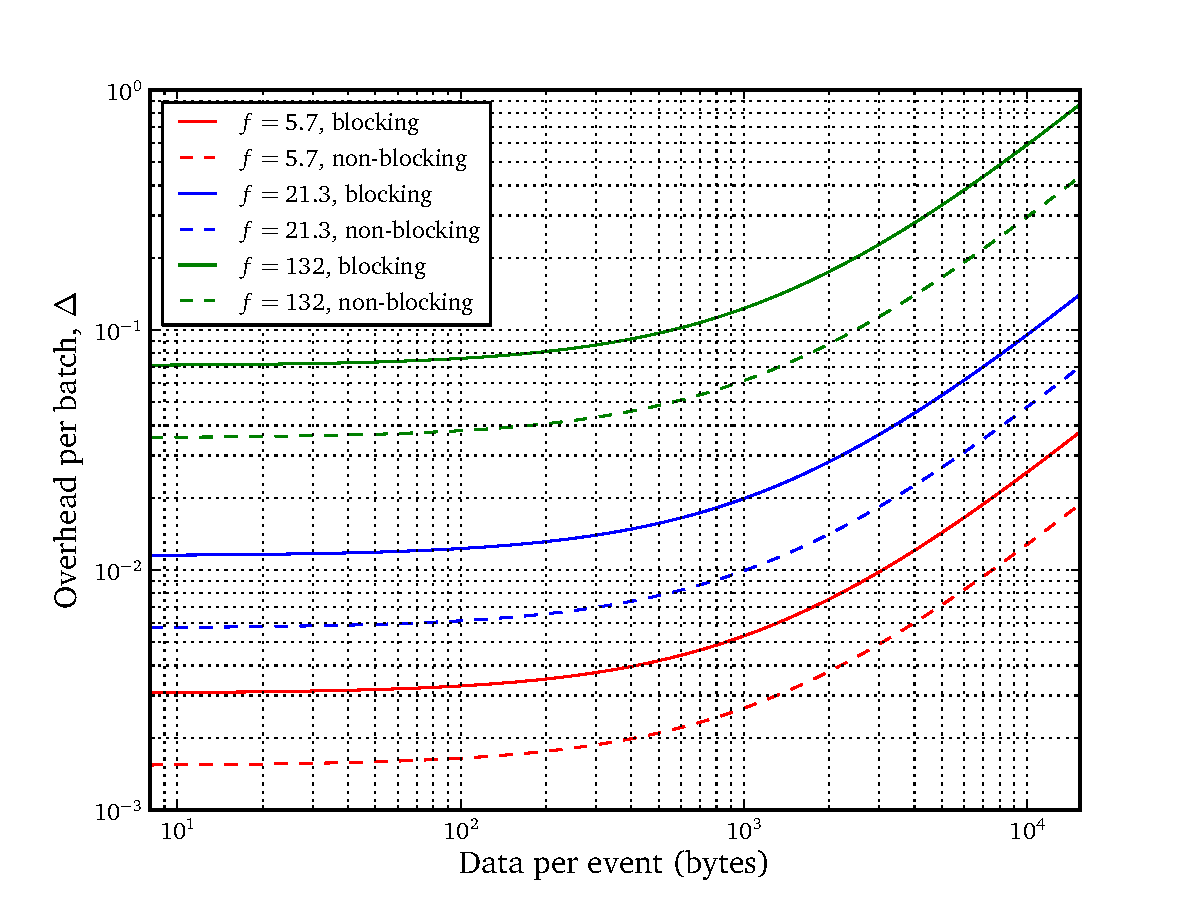
\includegraphics[width=4in]{figures/ch6/model_intrepid}
  \caption{Estimated tally server overhead for Intrepid Blue Gene/P
    supercomputer based on \eqref{eq:overhead-blocking} and
    \eqref{eq:overhead-nonblocking}.}
  \label{fig:model-intrepid}
\end{figure}

\begin{figure}[htb]
  \centering
  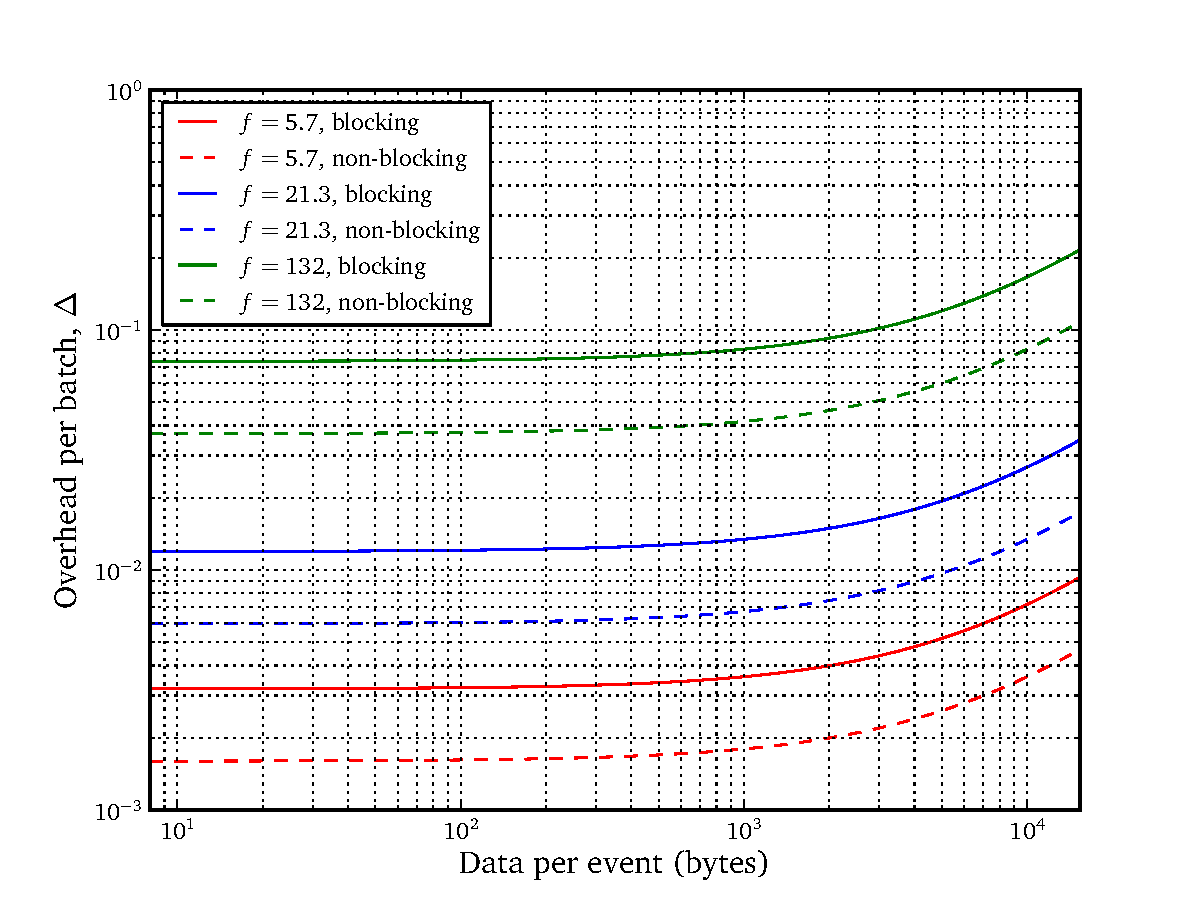
\includegraphics[width=4in]{figures/ch6/model_titan}
  \caption{Estimated tally server overhead for Titan Cray XK7 supercomputer
    based on \eqref{eq:overhead-blocking} and \eqref{eq:overhead-nonblocking}.}
  \label{fig:model-titan}
\end{figure}

We can also use equation \eqref{eq:support-ratio-blocking} to identify the
number of compute processors that can be supported by one server when using
blocking communication. For our worst case of $f = 21.3$ and $d = 15360$, the
constraint implies that on the Intrepid supercomputer we would need one server
for every 15 compute processors. On the Titan supercomputer, we would need one
server for every 58 compute processors for the same values of $f$ and $d$.

The predicted overhead due to tally servers based on the model in
\eqref{eq:overhead-blocking} and \eqref{eq:overhead-nonblocking} is quite
modest. In particular, over the range of parameter space that is of interest in
LWR analysis, the overhead is generally less than 10\% --- a very small price to
pay for the benefit of being able to have tallies of arbitrarily large size. The
promising results based on the theory presented here warrant an actual
implementation in a real Monte Carlo code. In \autoref{sec:implementation}, we
describe our implementation of this algorithm in the OpenMC Monte Carlo
code. Actual test results using the implementation in OpenMC are presented in
\autoref{sec:results}. Before we discuss the implementation and results,
however, we first discuss and analyze several considerations that may have an
influence on the achievable performance.

\subsection{Implications of total memory requirements}

One may have noted in the derivation of the performance model that, even though
the entire purpose of the algorithm is to allow for decomposition of the tally
memory, nowhere was the total memory requirement for the tallies taken into
account. In fact, one of the alluring aspects of the tally server algorithm is
that, in general, its performance does not depend on total amount of
memory. However, we must be careful in interpreting such a statement too broadly
as there are constraints on the memory.

The most obvious constraint is that the memory for each server must not exceed
the available memory on a single node. Let $M_t$ be the total memory required for
tallies, $M_s$ be the tally memory on each server, and $M_n$ be the available
memory on a node. This constraint implies that

\begin{equation}
  \label{eq:constraint-total}
  M_s < M_n.
\end{equation}

Another implicit assumption made in the course of the derivation was that the
message being sent was small relative to the tally memory on each
server. However, for a fixed tally size, the total tally memory on each server
will be inversely proportional to the total number of processors (assuming a
constant support ratio). Thus, as the total number of processors becomes very
large, the total memory on each server could hypothetically become smaller than
the message size for each scoring event. This situation would result in
increased overhead as it would necessitate sending more messages. A reasonable
constraint to impose is that the message size for each scoring event be smaller
that the tally memory of each server:

\begin{equation}
  \label{eq:constraint-message}
  d < M_s
\end{equation}

\noindent In practice, even $d = M_s$ can cause problems since a single message
can still overlap two servers. If we assume that the total memory required for
tallies is divided evenly over the tally servers, then the constraints in
\eqref{eq:constraint-total} and \eqref{eq:constraint-message} can be written in
combined form as

\begin{equation}
  \label{eq:constraint-memory}
  d < \frac{M_t}{s} < M_n.
\end{equation}

\noindent As we saw earlier, the upper limit on $d$ for our cases of interest is
15,360. Let us suppose that the memory on a single node is $M_n = 32 \cdot 10^9$
bytes. If the total memory of the tallies is $M_t = 500 \cdot 10^9$ bytes, then
\eqref{eq:constraint-memory} implies that

\begin{equation}
  \label{eq:constraint-example}
  15.6 < s < 3.26\cdot 10^6.
\end{equation}

\noindent Thus, we must have at least 16 servers in order for the memory
footprint of each to fit on a single node. This lower bound is quite easy to
achieve even on a small cluster. For the upper bound, if we have more the 3.26
million servers, each server would have too little data compared to the size of
a single message. At present, this limit puts no practical restrictions on our
use of the algorithm.

The constraint in \eqref{eq:constraint-memory} can also tell us, given a total
number of a tally servers, the range of total tally memory that can be
reasonably accommodated. Let us suppose we wanted to perform a simulation using
all nodes on the Mira Blue Gene/Q supercomputer at Argonne National
Laboratory. This supercomputer has 48 racks each having 1024 nodes, each of
which in turn has a 16 core processor for a total of 786,432 cores. Each node
has $M_n = 16 \cdot 10^9$ bytes of memory. Assuming a support ratio of $c/s =
15$, we would need 49,152 servers. Thus, \eqref{eq:constraint-memory} implies
that

\begin{equation}
  \label{eq:constraint-mira}
  755.0 \cdot 10^3 < M_t < 786.4 \cdot 10^{12}.
\end{equation}

\noindent For any reasonable simulation, the total memory of the tallies will
likely be somewhere between 755 kilobytes and 786 terabytes.

Admittedly, the foregoing analysis does not take into account the fact that
tally servers will have to share the memory of a single node with compute
processors. However, doing so would not change the overall conclusion that under
normal circumstances, the memory requirements are not a formidable challenge to
successfully employing the tally server algorithm.

\subsection{Dependence of \texorpdfstring{$\mu$ on $d$}{u on d}}

To this point, we have assumed that $\mu$ is independent of all other parameters
in our model. However, in most Monte Carlo transport codes, the rate at which
particles are simulated depends on how much data needs to be tallied. Hence
$\mu$ should really be a function of $d$, i.e. $\mu = \mu(d)$. In our case, $d$
will vary according to how many nuclides and scoring functions are being
tallied. For every nuclide reaction rate that needs to be tallied, it is
necessary to either calculate or look up a nuclide microscopic cross section at
the time of tallying. As a result, $\mu$ will depend linearly on $d$. If $\mu_0$
is the calculational rate with no tallies and $\mu_1$ is the average time to
process tally scores per byte, then we have that

\begin{equation}
  \label{eq:mu-function}
  \mu(d) = \mu_0 + d\mu_1
\end{equation}

\noindent Substituting $\mu(d)$ for $\mu$ in \eqref{eq:model-nonblocking}, the
tally server overhead using non-blocking communication would then be

\begin{equation}
  \label{eq:model-blocking-mud}
  \Delta_{\text{non-blocking}} = \frac{f}{\mu_0 + d\mu_1} \left ( \alpha + d\beta
    \right ).
\end{equation}

\noindent We see that the tendency would be to lessen the overhead as $d$ is
increased relative to the overhead in \eqref{eq:overhead-nonblocking}. In the
actual performance measurements discussed in \autoref{sec:results}, this effect
is accounted for explicitly by measuring $\mu$ over a range of $d$.

%%%%%%%%%%%%%%%%%%%%%%%%%%%%%%%%%%%%%%%%%%%%%%%%%%%%%%%%%%%%%%%%%%%%%%%%%%%%%%%%
\section{Implementation}
\label{sec:implementation}

\subsection{Description of algorithm}

The algorithm described in \autoref{sec:tally-server-algorithm} was implemented
in OpenMC; only modest changes were required to the source code to implement the
tally server algorithm. At initialization time, processes are divided into
compute processes and servers based on user input. If $p$ total processes and
$s$ servers are specified, then the processes whose MPI rank satisfies $i + 1
\mod s/p = 0$ are assigned as servers. Each user-defined tally has an array of
score objects whose length is the product of the number of filter bins
multiplied by the number of scoring functions. All scoring bins from
user-defined tallies are concatenated into one ``global'' tally score array
which is then divided equally over the servers. Finally, a look-up table is
constructed that relates indices in the global tally scores array to indices
within the scores array for each user-defined tally. The look-up table enables
the compute processes to determine which server they need to send scores to.

The necessary changes to the actual tallying subroutines that are used during
particle tracking follow directly from the discussion in
\autoref{sec:tally-server-algorithm}. As a summary, \autoref{alg:tallyserver}
shows a pseudocode outlining the salient points of the tally server algorithm as
implemented in OpenMC. There are a few important points to note regarding this
algorithm. Firstly, the array of scores created when a scoring event occurs
contains the scores for all specified scoring functions. This means that the
receiving server will increment multiple tally scores from a single
message. Also note that the servers must be informed of when a batch of
particles (or the simulation) has been completed as the servers are now
responsible for computing sums and sums of squares of the tally score bins in
order to calculate variances. At the end of the simulation, the servers must
collectively write the tally results to disk. This can be done efficiently using
parallel I/O techniques such as MPI-IO or parallel HDF5.

\begin{algorithm}
  \caption{Pseudocode for tally server algorithm}
  \label{alg:tallyserver}
  \begin{algorithmic}
    \If{compute process}
      \For{$i \gets 1 \textbf{ to } M$}
        \For{$j \gets 1 \textbf{ to } N/p$}
          \While{Particle $j$ is alive}
            \State Process next event
            \If{Event satisfies filter criteria}
              \State Create array for scores
              \ForAll{Scoring functions}
                \State Calculate score
                \State Add score to array
              \EndFor
              \State Determine server destination
              \State Send array to server
            \EndIf
          \EndWhile
        \EndFor
        \State Send `finished' message to server
      \EndFor
    \ElsIf{server}
      \Loop
        \State Receive message
        \If{End of batch}
          \State Accumulate tally scores
        \ElsIf{End of simulation}
          \State Accumulate tally scores
          \State {\bf exit loop}
        \Else
          \For{Score $i \gets 1 \textbf{ to } d$}
          \State Determine memory location $j$ to increment
          \State Increment tally $j$ with score $i$
          \EndFor
        \EndIf
      \EndLoop
      \State Write tally results to state point file
    \EndIf
  \end{algorithmic}
\end{algorithm}

\subsection{Potential optimizations}

\subsubsection{Explicit buffering}

In \autoref{alg:tallyserver}, an array of scores is sent to a server at every
single scoring event. If $f$ in \eqref{eq:overhead-blocking} or
\eqref{eq:overhead-nonblocking} is very large, this would clearly create a large
overhead regardless of whether the communication would be latency- or
bandwidth-dominated. One potential workaround for this situation would be to
explicitly buffer messages before sending. Rather than sending a message at
every scoring event, we could create a buffer array on the compute process for
each server that is some factor $\eta$ larger than the total number of scoring
functions for a tally. When the buffer array is full, it would then be sent to
the corresponding server. In this case, we have decreased $f$ by a factor of
$\eta$ and increased $d$ by the same factor. The predicted overhead using
non-blocking communication would then be
\begin{equation}
  \label{eq:overhead-nonblocking-buffer}
  \Delta_{\text{non-blocking}} = \frac{f}{\eta\mu} \left ( \alpha + d\eta\beta
  \right ) = \frac{f}{\mu} \left ( \frac{\alpha}{\eta} + d\beta \right ).
\end{equation}

\noindent We see in \eqref{eq:overhead-nonblocking-buffer} that the latency term
has been reduced by a factor of $\eta$, but the bandwidth term is
unchanged. Since the main case of interest (depletion of an LWR model) was shown
to be in the bandwidth-dominated region for contemporary supercomputers, the
extra effort of implementing explicit buffering did not seem to justify the
performance benefit for cases that are latency-dominated. This is especially
true given that, as we will see in \autoref{sec:results}, the overhead for
latency-dominated cases is extremely small. Explicit buffering could also
hypothetically limit network contention by reducing the total number of
messages, but this effect is hard to quantify.

\subsubsection{Combining successive scoring events}

A small variation on the explicit buffering concept described in the previous
section is to combine successive scores that match the same filter criteria. Let
us suppose that for a tally with scoring bins $b_i, i = 1, \dots, k$, we have
$n$ consecutive scoring events that match the same filter criteria. Let
$x_{i,j}$ be the $i$th score for the $j$th event. In the basic algorithm, we
send a message containing the values $x_{1,j}, x_{2,j}, \dots, x_{k,j}$ to a
server for each scoring event. Then the server adds each score to the
appropriate scoring bin $b_i \gets b_i + x_{i,j} \forall i$. Rather than sending
$n$ messages and having the server accumulate each array of scores, the compute
processes can combine consecutive scores and subsequently send the sum to a
server to be accumulated. Each compute process would calculate $x_i' = \sum_j
x_{i,j}$, and the server would accumulate $b_i \gets b_i + x_i'$. This scheme
effectively reduces the number of scoring events per particle, $f$.

To obtain a simple estimate of the potential reduction in $f$, let us consider
the case of track-length tallies in the fuel region. Any time a particle
scatters within the fuel region, it will result in two separate tracks. The
tally scores from these separate tracks could be combined and sent to a server
in one message. This implies that the effective number of scoring events, $f'$,
is then
\begin{equation}
  f' = \left ( 1 - \frac{\Sigma_s \phi}{\Sigma_t \phi} \right ) f
\end{equation}
where $\Sigma_s \phi$ is the scattering reaction rate in the fuel and $\Sigma_t
\phi$ is the total reaction rate in the fuel. For the Monte Carlo performance
benchmark $\Sigma_s \phi/\Sigma_t \phi = 0.23$, so $f$ would be reduced about
23\%.

\subsubsection{Topologically-aware layouts}

To maximize network bandwidth and minimize latency, the mapping of processes to
processor cores could hypothetically be optimized based on the topology of the
particular machine the algorithm is implemented on. We chose a naïve
implementation that is unaware of topology to ensure portability across
different architectures and to demonstrate that successful use of the algorithm
does not require such optimizations.

%%%%%%%%%%%%%%%%%%%%%%%%%%%%%%%%%%%%%%%%%%%%%%%%%%%%%%%%%%%%%%%%%%%%%%%%%%%%%%%%
\section{Results}
\label{sec:results}

The performance model developed in \autoref{sec:tally-server-analysis} is dependent on a
variety of parameters. On any given computer, $\alpha$, $\beta$, and $\mu$ are
effectively constant. The remaining parameters can be manipulated by varying the
definition of the tallies and the job parameters. Thus, to fully test the
performance of the tally server implementation, a parameter study should be
carried out by running a series of simulations varying the parameters $p$, $s$,
$f$, and $d$.

One could argue that based on \eqref{eq:overhead-nonblocking}, it should not be
necessary to include $p$, $c$, or $s$ in the parameter study since the overhead
does not explicitly depend on those parameters. However,
\eqref{eq:overhead-nonblocking} was derived assuming that the support ratio
attains its maximum based on the inequality in
\eqref{eq:support-ratio-nonblocking}. In practice, it's not possible to know
\emph{a priori} what the maximum attainable support ratio is and thus it is
instructive to test this directly. While the performance depends on $f$ in
general, our primary interest is tally events in the fuel region. As a result,
we performed a parameter study using the modified version of OpenMC varying $p$,
$c/s$, and $d$ only.

First, a number of ``baseline'' simulations of the Monte Carlo performance
benchmark were run to determine how $\mu$ varies with increasing $d$, and hence
how $t_0$ varies with increasing $d$. The baseline simulations were run without
tally servers to capture only the increase in simulation time due to cross
section look-ups for tallies. On both the Titan supercomputer, the baseline
simulations were run with 16 processors with a total of 32,000 particles per
batch. Ten batches were run both without tallies (referred to as \emph{inactive
  batches}) and with tallies (\emph{active batches}). These values were found to
be adequate to accurately profile performance. On the Intrepid supercomputer,
the baseline simulation was run with a single processor with 2000 particles per
batch. Again, ten batches were run first without and then with tallies. For each
case, a tally was set up with a mesh filter and a second filter to match only
events within the fuel volume. The scoring functions requested were the flux,
total reaction rate, scattering rate, absorption rate, fission rate, and neutron
production rate for varying numbers of nuclides, starting with 5 nuclides and
doubling the number of nuclides up to 320. Thus, the amount of data sent at each
event varied from 240 bytes up to 15.36 kilobytes. \autoref{fig:mu-d} shows the
observed dependence of $\mu$ on $d$ normalized to the $d=5$ case.

\begin{figure}
  \centering
  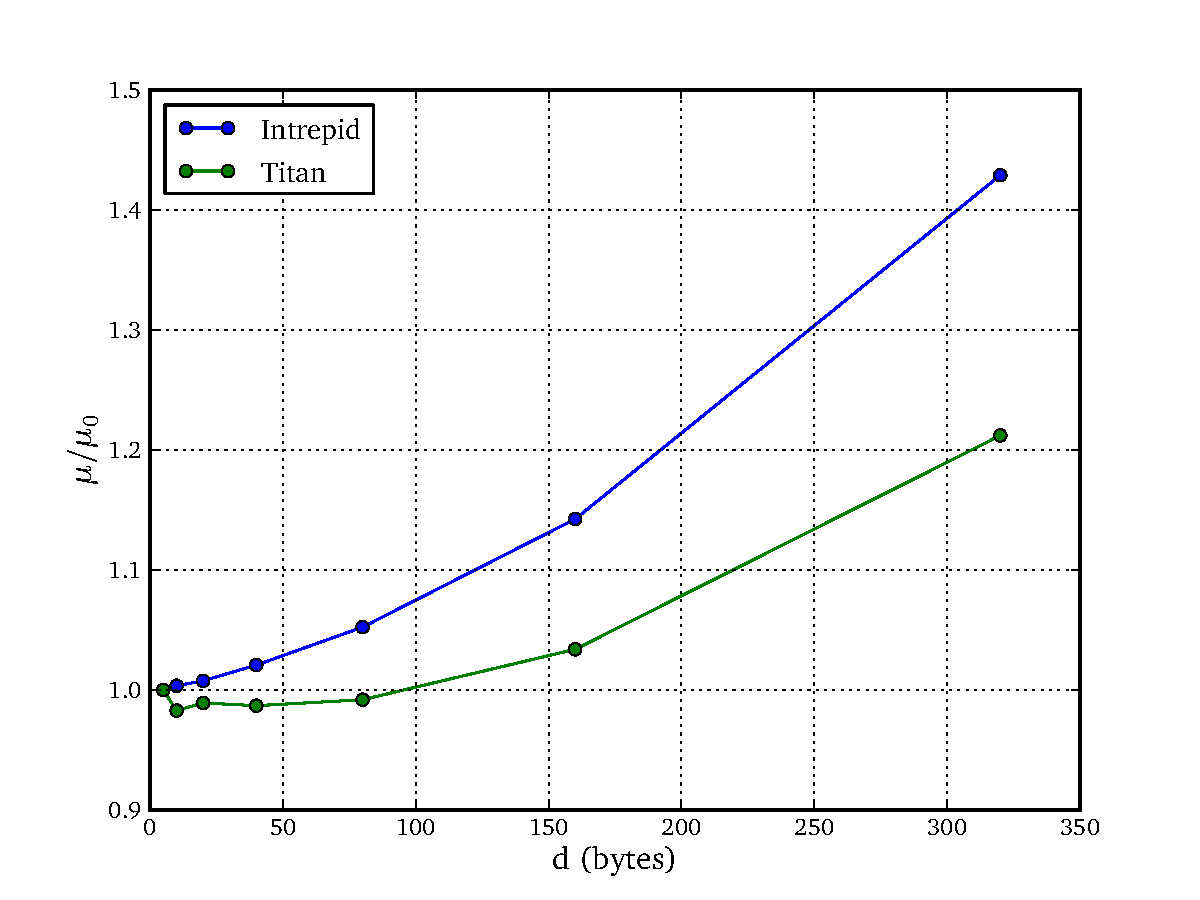
\includegraphics[width=4.0in]{figures/ch6/results_baseline.pdf}
  \caption{Observed dependence of $\mu$ on the amount of data tallied, $d$, on
    Intrepid and Titan.}
  \label{fig:mu-d}
\end{figure}

The parameter study using tally servers on the Intrepid supercomputer consisted
of 168 simulations with each combination of the following parameters: $p =
16,32,64,128, \allowbreak 256,512$, $c/s = 1,3,7,15$, and $d = 240, 480, 960,
1920, 3840, 7680, 15360$. Like the baseline cases, the runs with tally servers
had 10 inactive batches, 10 active batches, and $N/p = 500$. The effective
overhead from tally servers was determined in the following manner. First, the
expected overhead due to looking up cross sections during tallying was
subtracted from the active batch time based on the results from the baseline
cases. Then, the adjusted simulation time in active batches was divided by the
inactive batch time to determine the overhead in active batches. This
essentially represents an estimate for the second term in \eqref{eq:model},
i.e. it does not account for the fact that we have fewer compute
processors. However, if we know $p$ and $c$, that source of overhead is trivial
to calculate --- it is really the extra overhead from message-passing that we
are interested in. The overhead calculated in this manner for $c/s = 1$, $c/s =
3$, $c/s = 7$, and $c/s = 15$ is shown in \autoref{fig:intrepid-r1},
\autoref{fig:intrepid-r3}, \autoref{fig:intrepid-r7}, and
\autoref{fig:intrepid-r15}, respectively.

\begin{figure*}[!th]
  \makebox[\textwidth][c]{
  \begin{floatrow}[2]
    \ffigbox[\FBwidth] {
          \caption{Tally server overhead on Intrepid Blue Gene/P as a function
            of data per event with $c/s = 1$.}
          \label{fig:intrepid-r1}
        } {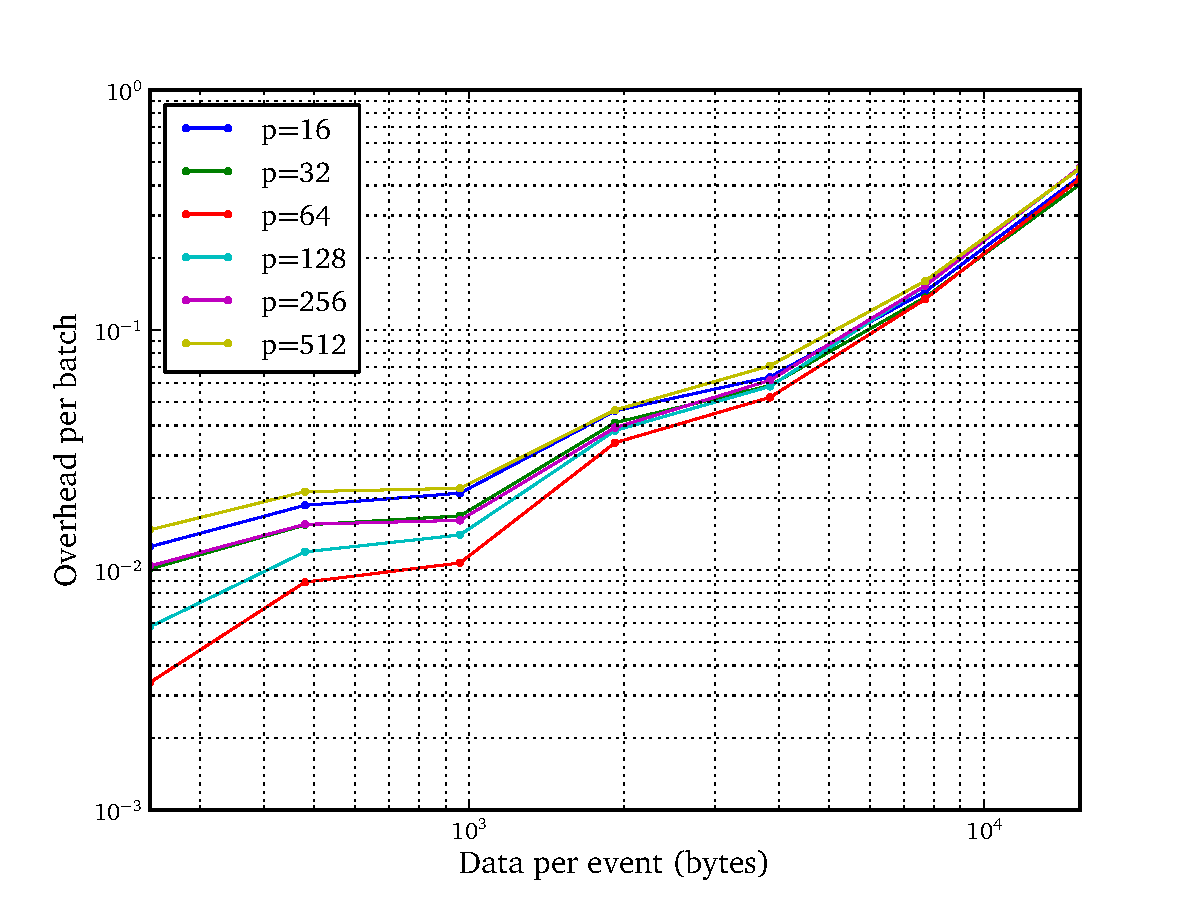
\includegraphics[width=3.4in]{figures/ch6/results_intrepid_r1}}
    \ffigbox[\FBwidth] {
          \caption{Tally server overhead on Intrepid Blue Gene/P as a function
            of data per event with $c/s = 3$.}
          \label{fig:intrepid-r3}
        } {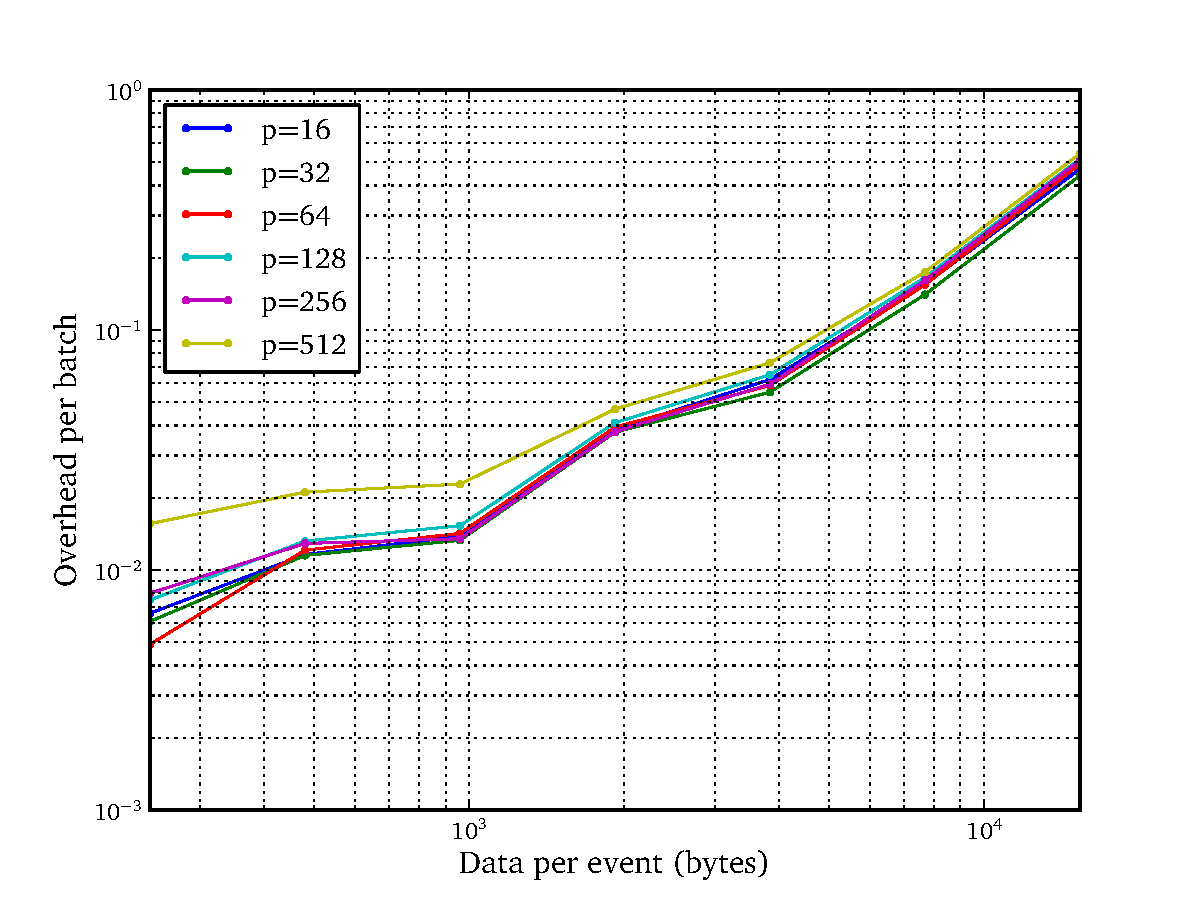
\includegraphics[width=3.4in]{figures/ch6/results_intrepid_r3}}
  \end{floatrow}
  }
  \begin{floatrow}
    \ffigbox[\FBwidth] {
          \caption{Tally server overhead on Intrepid Blue Gene/P as a function
            of data per event with $c/s = 7$.}
          \label{fig:intrepid-r7}
        } {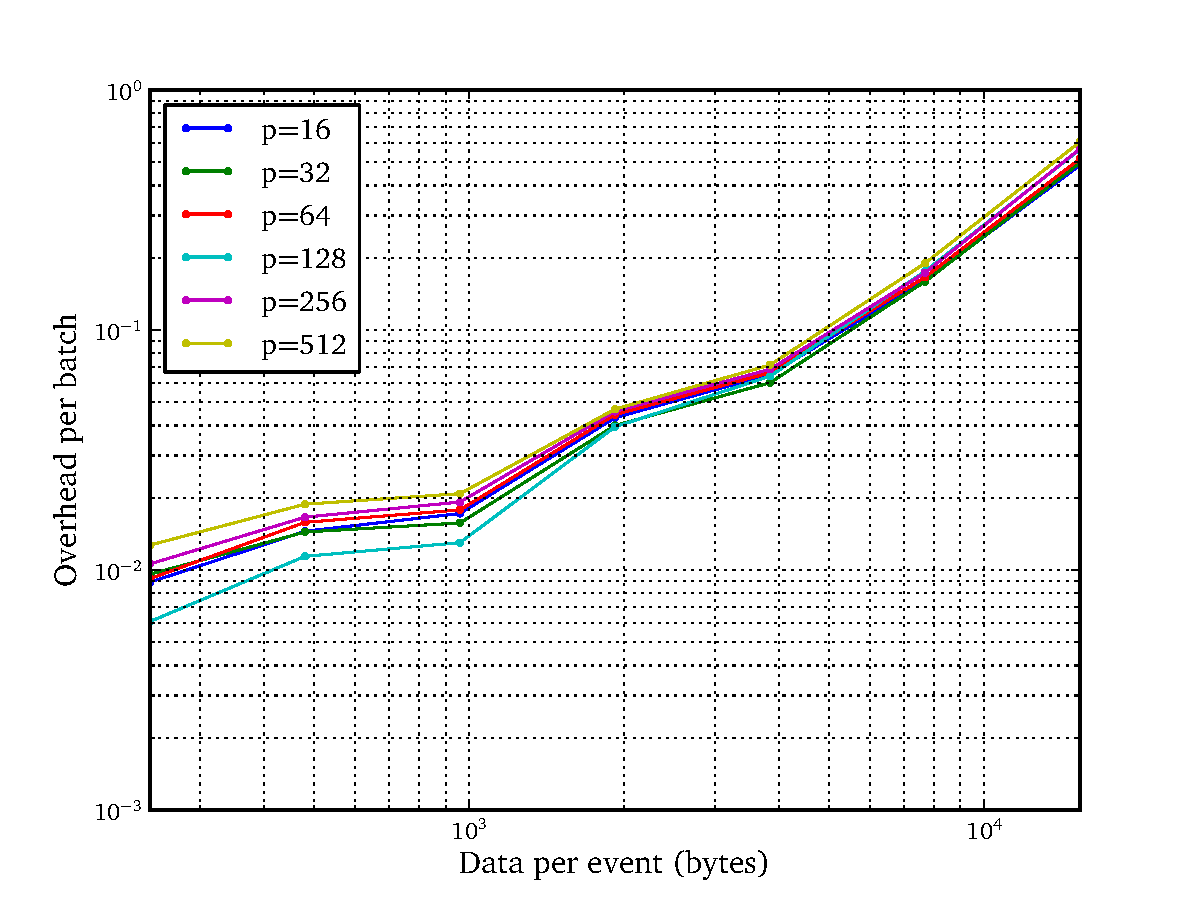
\includegraphics[width=3.4in]{figures/ch6/results_intrepid_r7}}
    \ffigbox[\FBwidth] {
          \caption{Tally server overhead on Intrepid Blue Gene/P as a function
            of data per event with $c/s = 15$.}
          \label{fig:intrepid-r15}
        } {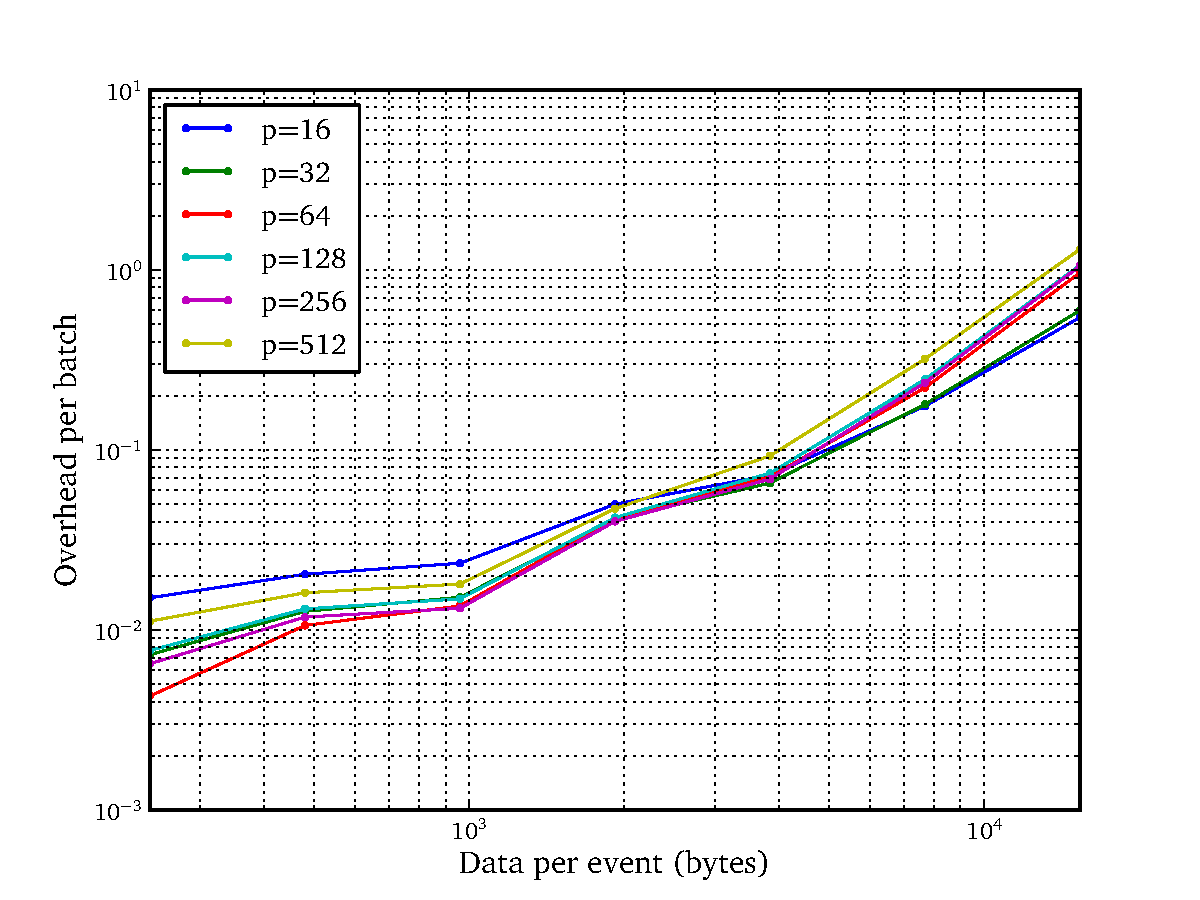
\includegraphics[width=3.4in]{figures/ch6/results_intrepid_r15}}
  \end{floatrow}
\end{figure*}

It is also of interest to observe the behavior of the tally server overhead with
increasing numbers of total processors. Recall that the performance model
predicts that the overhead should not depend on the number of processors
used. \autoref{fig:intrepid-cs} shows the overhead plotted as a function of $p$
for cases with $d = 15360$. We see that the overhead does not increase
appreciably for $c/s = 1, 3, 7$. However, for $c/s = 15$ the performance begins
to degrade. This may indicate that on Intrepid, this support ratio is not quite
sufficient for all servers to keep up with the volume of messages. Since the
model assumptions regarding achievable bandwidth do not account for contention,
such deviation from the model is not unexpected.

\begin{figure}[!tbh]
  \centering
  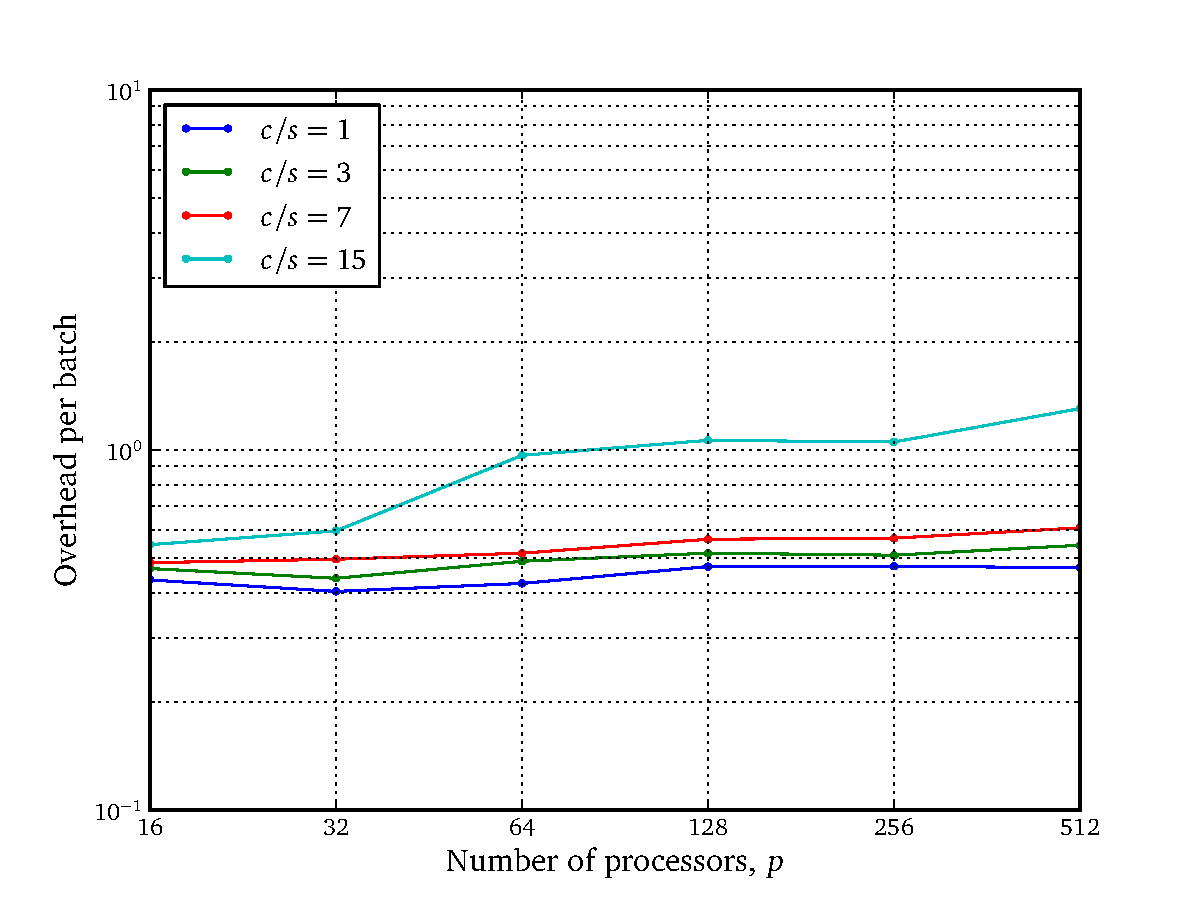
\includegraphics[width=4in]{figures/ch6/results_intrepid_cs}
  \caption{Tally server overhead on Intrepid Blue Gene/P as a function of $p$
    for $d = 15360$.}
  \label{fig:intrepid-cs}
\end{figure}

Another parameter study using tally servers on the Titan supercomputer consisted
of 196 simulations with each combination of the following parameters: $p =
16,32,64,128,256,512,1024$, $c/s = 1,3,7,15$, and $d = 240, 480, 960, 1920,
3840, 7680, 15360$. Again, the runs with tally servers had 10 inactive batches,
10 active batches, and $N/p = 1000$. The effective overhead from tally servers
was determined as described for the study on Intrepid. The calculated overhead
for $c/s = 1$, $c/s = 3$, $c/s = 7$, and $c/s = 15$ is shown in
\autoref{fig:titan-r1}, \autoref{fig:titan-r3}, \autoref{fig:titan-r7}, and
\autoref{fig:titan-r15}, respectively.

\begin{figure*}[!tbh]
  \makebox[\textwidth][c]{
  \begin{floatrow}[2]
    \ffigbox[\FBwidth] {
          \caption{Tally server overhead on Titan Cray XK7 as a function
            of data per event with $c/s = 1$.}
          \label{fig:titan-r1}
        } {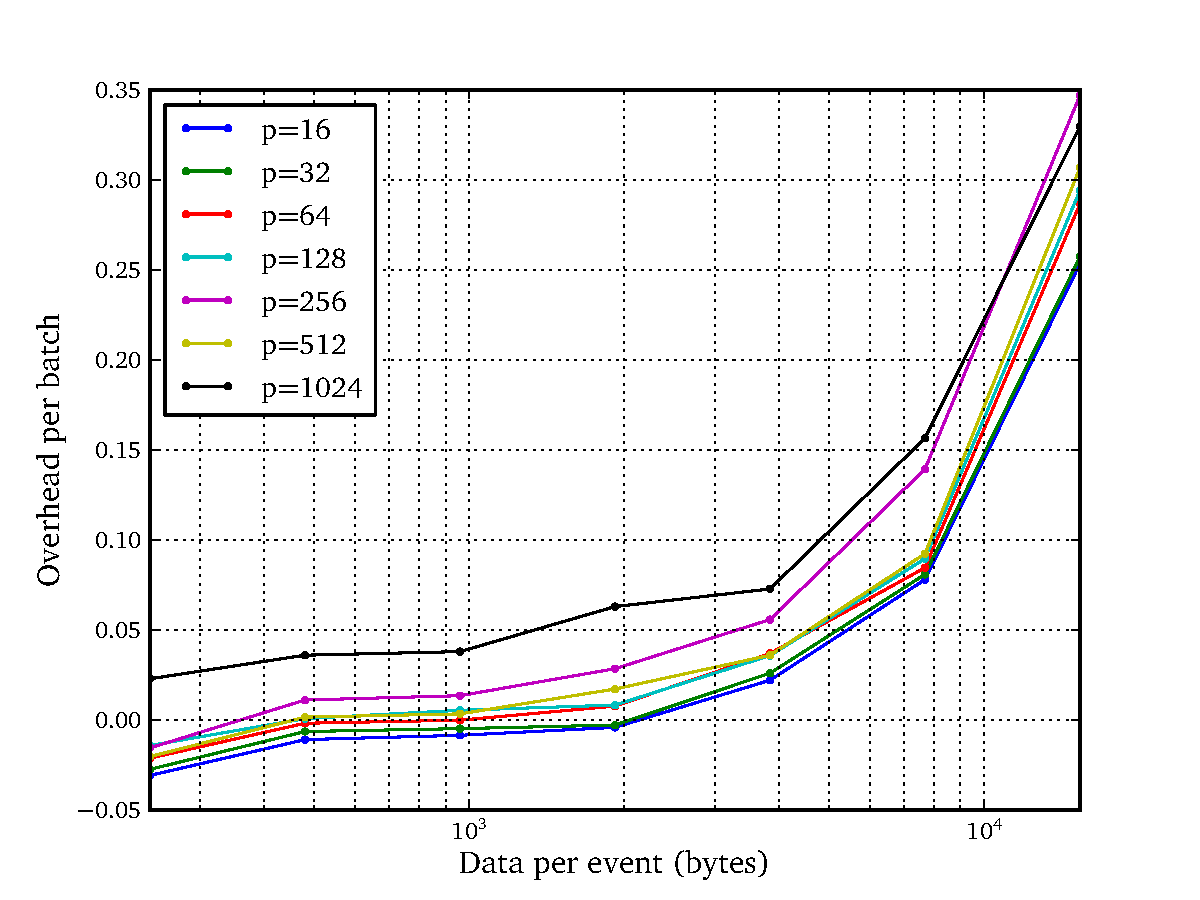
\includegraphics[width=3.4in]{figures/ch6/results_titan_r1}}
    \ffigbox[\FBwidth] {
          \caption{Tally server overhead on Titan Cray XK7 as a function
            of data per event with $c/s = 3$.}
          \label{fig:titan-r3}
        } {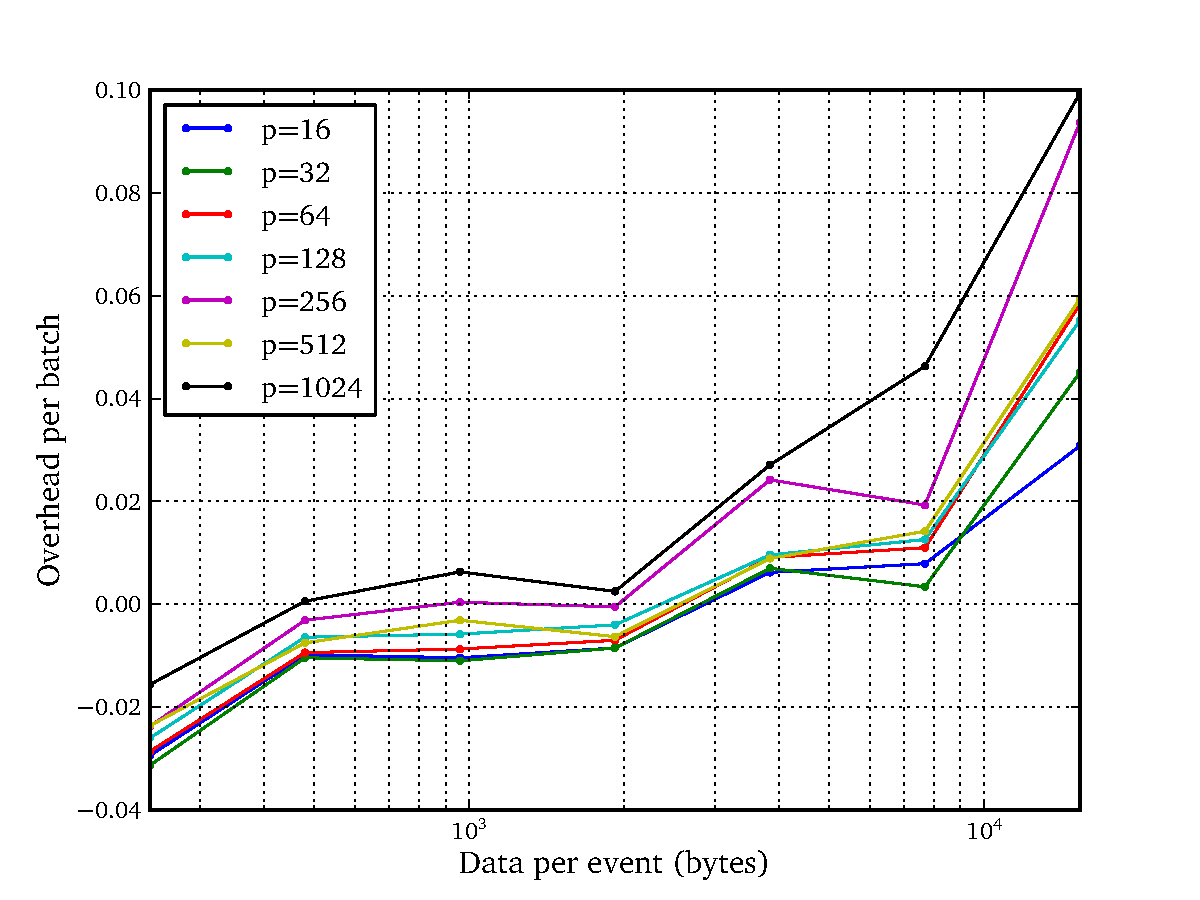
\includegraphics[width=3.4in]{figures/ch6/results_titan_r3}}
  \end{floatrow}
  }
  \begin{floatrow}
    \ffigbox[\FBwidth] {
          \caption{Tally server overhead on Titan Cray XK7 as a function
            of data per event with $c/s = 7$.}
          \label{fig:titan-r7}
        } {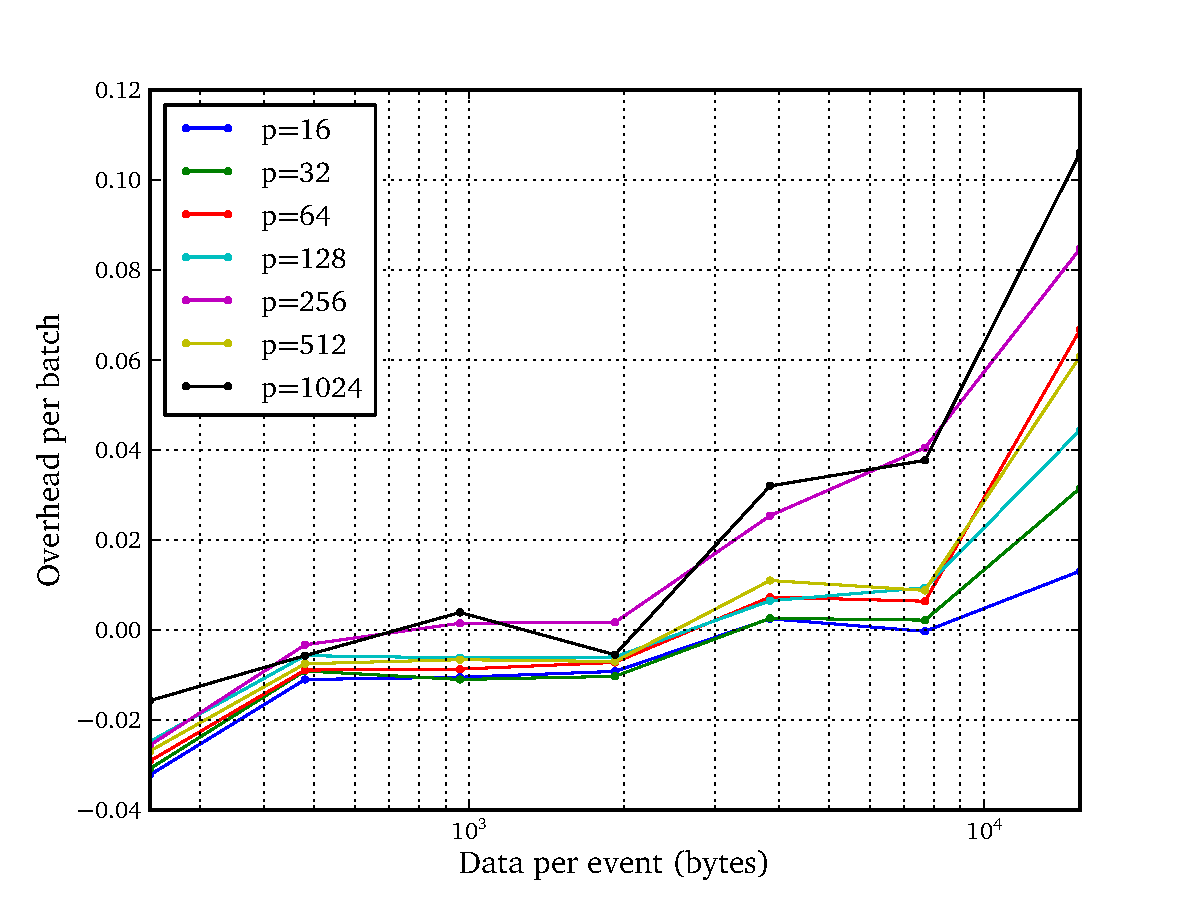
\includegraphics[width=3.4in]{figures/ch6/results_titan_r7}}
    \ffigbox[\FBwidth] {
          \caption{Tally server overhead on Titan Cray XK7 as a function
            of data per event with $c/s = 15$.}
          \label{fig:titan-r15}
        } {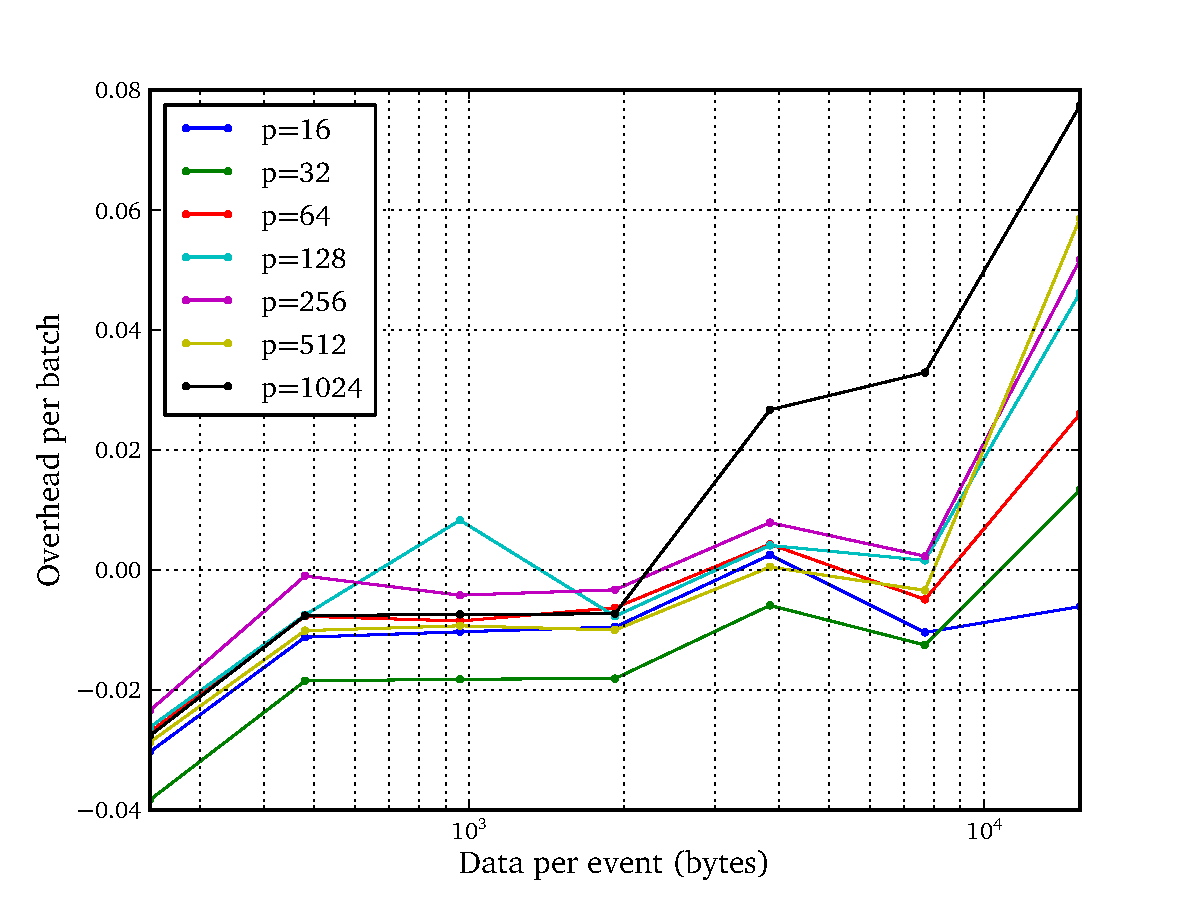
\includegraphics[width=3.4in]{figures/ch6/results_titan_r15}}
  \end{floatrow}
\end{figure*}

Similar to \autoref{fig:intrepid-cs}, we can look at the behavior of the tally
server overhead on Titan with increasing $p$. \autoref{fig:titan-cs} shows the
overhead plotted as a function of $p$ for cases with $d = 15360$. We see that
the overhead is relatively stable with increasing $p$. However, the cases with
$c/s = 1$ are clearly outliers with much higher overhead than the other
cases. This is likely due to network contention since the $c/s = 1$ cases result
in half of the processor cores on each node sending messages simultaneously. To
understand in greater depth the variability of the overhead as a function of,
e.g., the support ratio would likely require a deeper investigation of a
particular architecture, including topology-aware algorithms and a more
sophisticated model for network contention. These studies are beyond the scope
of the present work and are not central to addressing the key questions we set
out to study.

\begin{figure}[!tbh]
  \centering
  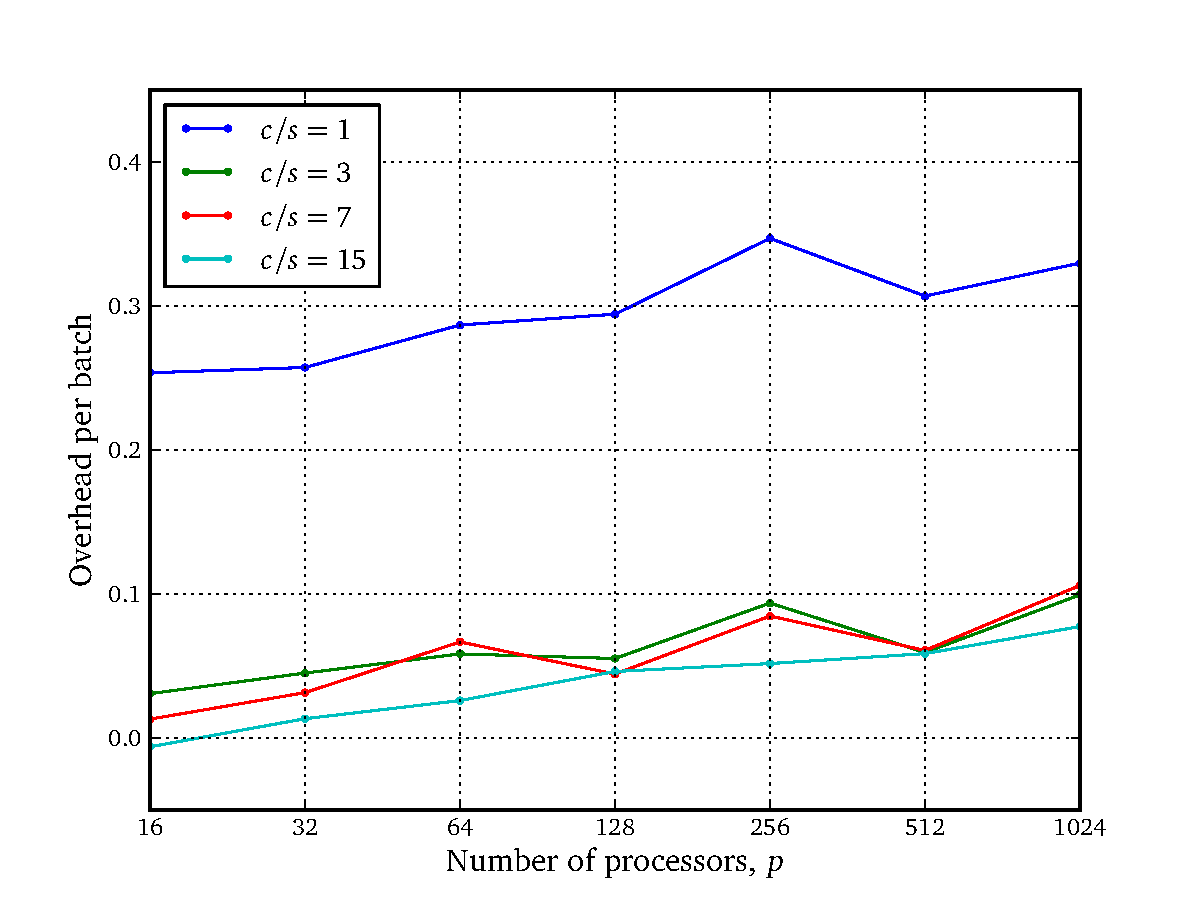
\includegraphics[width=4in]{figures/ch6/results_titan_cs}
  \caption{Tally server overhead on Titan Cray XK7 as a function of $p$ for $d =
    15360$.}
  \label{fig:titan-cs}
\end{figure}

%%%%%%%%%%%%%%%%%%%%%%%%%%%%%%%%%%%%%%%%%%%%%%%%%%%%%%%%%%%%%%%%%%%%%%%%%%%%%%%%
\section{Conclusions}

An algorithm for decomposing large tally data in Monte Carlo particle transport
simulations was proposed, analyzed, and implemented/tested in OpenMC. The
algorithm relies on disjoint sets of compute processes and servers of which the
former simulate particles moving through the geometry and the latter runs in a
continuous loop receiving scores from the compute processors and incrementing
tallies. This algorithm potentially allows the end user to dramatically increase
the overall tally memory footprint and therefore enables the potential to carry
out full core fuel depletion calculations.

The proposed algorithm is only of practical value if the communication penalty
resulting from tally decomposition is reasonable relative to the key timescales
of the problem. We carried out an analysis to that end and showed in
\autoref{sec:tally-server-analysis} that for a range of parameters relevant to 
LWR analysis, the tally server algorithm should perform with minimal overhead on
contemporary supercomputers regardless of the message-passing semantics. An
implementation of the algorithm in OpenMC was tested on the Intrepid and Titan
supercomputers and was demonstrated to perform well over a wide range of the
parameters. We can conclude that even with no further improvements in the
algorithm or its implementation in OpenMC, it could be successfully used to
analyze LWR models with a level of fidelity that was heretofore not possible due
to the need to replicate memory across all processors. It is likely that future
developments in Monte Carlo methods for reactor analysis and improvements in
computer architectures will only improve the performance of the tally server
algorithm over time.

One point that was made earlier was that the algorithm presented here does not
reduce the burden of large cross section data. For realistic reactor analysis,
cross section data may well reach into the hundreds of gigabytes owing to the
fact that cross section libraries would be needed at a multitude of
temperatures. In \autoref{sec:cross-section-memory}, we had discussed two
promising efforts in the area of on-the-fly evaluation of effective cross
sections at any temperature --- the work of Yesilyurt on on-the-fly Doppler
broadening \cite{nse-yesilyurt-2012} and the work of Viitanen on explicit
temperature treatment \cite{nse-viitanen-2012}. The latter development would
enable simulation using 0 K cross sections but with a significant performance
penalty. In general, this and other improvements in physics methods will likely
lead to slower simulations but with higher fidelity. From the perspective of the
tally server model, these developments will increase $\mu$ and consequently
decrease the communication overhead.

On the hardware end, improvements in supercomputer architectures may continue to
reduce network latency and improve bandwidth, at least in the short-term. Again,
this will largely benefit the tally server algorithm. Since incrementing tallies
can naturally be expressed as a fetch-and-add atomic operation, there is also
potential to exploit remote direct memory access (RDMA) operations either
explicitly (e.g., using MPI-2) or implicitly through a partitioned global
address space (e.g., Fortran co-arrays). Modern network interconnects should be
able to take advantage of RDMA operations. In addition, the requirement that
servers and compute processes be disjoint could be obviated by the use of RDMA,
potentially offering further reductions in overhead.

One potential downside to the algorithm presented here is that it considerably
complicates the use of threading via OpenMP. The most natural means of obtaining
thread-level parallelism in a Monte Carlo particle transport simulation is to
divide particles within a batch over multiple threads. Normally, no
communication occurs until the end of a batch when it is necessary to
synchronize fission bank sites and tallies. However, with the inclusion of tally
servers, it would then be necessary for each thread to participate in
message-passing. Further algorithmic innovations will need to be explored to
efficiently combine a tally server model with on-node shared-memory parallelism.

As a final comment, one should recognize the fact that the algorithm presented
here has primarily been presented with a focus and intent on applications in LWR
analysis. For other types of analysis performed with Monte Carlo, it may turn
out that the tally server algorithm does not make sense.

\chapter{Conclusions}
\label{chap:conclusions}

Monte Carlo particle transport methods are being considered as a viable option
in the future for high-fidelity simulation of nuclear reactors. This is, in
part, thanks to the enormous advances in high performance computing. If parallel
methods were not exploited, the sheer number of floating point operations
(FLOPs) required to reduce stochastic uncertainty to acceptable levels when
using Monte Carlo would require unacceptably long simulation time. However, the
present availability of supercomputers with hundreds of thousands or millions of
processor cores means that, solely from the perspective of FLOPs required,
solution to LWR problems using Monte Carlo could hypothetically be done in a
short time.

Lest we be fooled into thinking floating point operations are the only challenge
to overcome, let us remind ourselves that they are but one small piece of the
puzzle --- there are a variety of algorithmic and architectural challenges that
will not be easy to solve; an excellent summary of these issues, especially as
they apply to full-core LWR calculations, has recently been given by Martin
\cite{net-martin-2012}. The objective of this thesis was to make headway towards
overcoming some of these challenges.

In \autoref{chap:intro}, an overview of four contemporary issues preventing
Monte Carlo simulations of realistic LWR models was given: source convergence,
cross section memory requirements, tally memory requirements, and degradation in
parallel efficiency. In the following sections, we will summarize the status of
and progress that has been made in each area as well as what ongoing work will
still be needed in order to reach the goal of performing reactor analysis with
Monte Carlo.

\section{Source Convergence}

One area that has received quite a bit of attention in the last decade is source
convergence in Monte Carlo calculations. There are, in a sense, two separate
issues relating to source convergence. The first is being able to assess the
convergence of the source distribution, i.e. because the source distribution is
a collection of finite points in multiple dimensions, how can one assure that it
has reached stationarity in the method of successive generations. For a scalar
value, such as the global eigenvalue, it is intuitive to merely look a line plot
of its value versus the number of batches.

The second issue is accelerating convergence of the source distribution. Until
the source has converged in a Monte Carlo eigenvalue calculation, it is not
possible to accumulate tallies. Thus, the inactive batches are ``wasted'' as it
were. If a method could be employed to reduce the number of inactive batches, we
would save the wasted calculational time. Both issues are made worse by a high
dominance ratio; this is unfortunately the case in a full-core reactor where the
dominance ratio can be very close to unity.

\subsection{Status}

The pioneering work of Ueki and Brown \cite{trans-ueki-2002, physor-brown-2006}
has helped introduce and gain acceptance of the Shannon entropy, a scalar metric
based on information theory, as a proper means for assessing convergence of the
source distribution. Shannon entropy has now been implemented in most modern
Monte Carlo codes, including OpenMC (see \autoref{sec:shannon-entropy}). While
Shannon entropy will work for nearly all models, it may be ill-suited for very
large, loosely-coupled models such as a spent fuel array; for these problems,
research efforts are looking into mesh-based convergence diagnostics
\cite{mc-she-2011}.

Various methods have been proposed, tested, and implemented in Monte Carlo codes
for accelerating source convergence. In the author's opinion, one of the more
promising methods, which is widely employed in deterministic calculations, is
coarse mesh finite difference. The basic idea is to use volume-integrated
reaction rates and partial currents on mesh surfaces from Monte Carlo tallies to
solve a low-order system. This method has been proven to be quite effective in
reducing the number of inactive batches in Monte Carlo eigenvalue
calculations \cite{physor-lee-2012}.

We see then that significant progress has been made in the area of source
convergence in Monte Carlo eigenvalue calculations. For full-core LWR models,
CMFD can be used to accelerate source convergence, and Shannon entropy can be
used to assess source convergence. As a result, it was not an objective of this
thesis to pursue further work in the area of source convergence.

\subsection{Future Work}

Nevertheless, there are still a number of interesting areas of research
pertaining to source convergence. While source convergence can be assessed using
Shannon entropy, there is as-of-yet no viable method for diagnosing
undersampling. Undersampling is a phenomenon whereby local tallies may be
systematically biased as a result of not using enough particles per batch
\cite{nse-ueki-2005, nse-ueki-2008}. To the author's knowledge, only one method
for undersampling diagnosis has been proposed in the literature
\cite{jnst-ueki-2011}, but it unfortunately would not be feasible in a realistic
calculation due to memory requirements. Moreover, while the bias in global
eigenvalue is fairly well understood \cite{ane-brissenden-1986} and known to be
small, no study has systematically looked at bias in local tallies due to
undersampling.

In the area of source convergence acceleration, one current ``hot topic''
pertaining to CMFD is determining the best way to generate multigroup parameters
for the diffusion solver. In particular, generating multigroup diffusion
coefficients from a Monte Carlo code can be problematic. A number of research
efforts are currently looking at methods for generating diffusion coefficients
in the hope that more accurate parameters will lead to better convergence
properties \cite{ane-fridman-2011, nse-pounders-2009}. Researchers are also
looking at other low-order methods for accelerating convergence.

\section{Parallel Efficiency}

Solution of full-core LWR problems will require an enormous number of floating
point operations and will thus necessitate the use of thousands or millions of
processors in parallel. However, with current parallel algorithms, a serious
degradation in parallel efficiency will likely be experienced when one tries to
use even thousands of processors \cite{physor-hoogenboom-2012}. To reiterate,
two of the root causes for this degradation are reduction of tallies and
synchronization of the fission source at each batch in an eigenvalue
calculation. One of our major objectives in this work has been to develop
algorithms that ameliorate the degradation of parallel efficiency at large
numbers of processors.

\subsection{Contributions of Present Work}

In \autoref{chap:fission-bank}, a nearest-neighbor algorithm was proposed and
subsequently implemented in the OpenMC Monte Carlo code. This algorithm takes
advantage of the fact that many of the fission sites produced on one processor
can be used as source sites on that same processor --- in doing so, it avoids
unnecessary communication between processors. A theoretical analysis of the
algorithm shows that the expected cost is $O(\sqrt{N})$, $N$ being the number of
particles per generation, whereas traditional master-slave algorithms are $O(N)$
at best, and possibly even $O(N \log_2 N)$. The algorithm was tested on two
contemporary supercomputers, the Intrepid Blue Gene/P at ANL and the Titan Cray
XK7 at ORNL, and demonstrated nearly linear parallel scaling up to 163,840
processor cores. There is no reason to believe that the nearest-neighbor
algorithm will not scale to even greater processor counts.

In \autoref{chap:tally-reduction}, an algorithm for reducing network
communication arising from tally reduction was analyzed and, again, implemented
in OpenMC. The basic idea is conceptually very simple --- the grouping of
particles histories into batches for the sake of calculating variance is
arbitrary. The proposed algorithm groups only particle histories on a single
processor and in doing so prevents all network communication for tallies until
the very end of the simulation. In a large scale parallel calculation of, say, a
realistic LWR model, it is likely that enough processors will be used to obtain
a sufficient number of realizations of the random variables. This algorithm was
tested in OpenMC on the Monte Carlo performance benchmark on a cluster at MIT,
and it was shown that network communication was substantially reduced.

Together, the algorithms presented in \autoref{chap:fission-bank} and
\autoref{chap:tally-reduction} should enable very high parallel efficiencies to
be attained for eigenvalue calculations using the method of successive
generations. These algorithms have been published in \cite{nse-romano-2012} and
\cite{trans-romano-2012}, respectively.

\subsection{Future Work}

There are a few potential shortcomings of the nearest-neighbor fission bank
algorithm. One that was mentioned in the conclusions of
\autoref{chap:fission-bank} is that the algorithm would preclude the use of load
balancing via existing algorithms for heterogeneous computer architectures. A
simple method to provide load balancing in such situations based on ``tuning''
the algorithm was suggested, but it has never been tested. Additionally, the
nearest-neighbor algorithm may be very difficult to combine with any domain
decomposition scheme since the order of fission bank sites would necessarily
depend on their spatial coordinates. If domain decomposition is ever to be used
for calculations with tens of thousands of processors or more, this issue will
likely need to be addressed.

The tally reduction algorithm is robust; we see no immediate need to pursue
further work on it. Perhaps one downside of the method is that it will not
exactly reproduce the variance of a calculation in which particle histories are
batched according to single fission generations. However, this is no different
than saying that any calculation that uses batching will not reproduce the
variance exactly. It was argued that, in the absence of intergenerational
correlation, the expected value of the variance is the same regardless of the
batching. In fact, batching particle histories across fission generations will
produce more reliable estimates of variance in an eigenvalue calculation since
intergenerational correlation effects are avoided in doing so.

\section{Cross Section Memory}

In order to perform a realistic simulation of a reactor at power, it is
important to account for the dependence of interaction cross sections on
temperature. In \autoref{sec:cross-section-memory}, this was discussed at
length, and we found that the memory requirements resulting from storing cross
sections at a multitude of temperatures could be as high as hundreds of
gigabytes. Thus, methods are needed to reduce or decompose the cross section
data. We reiterate that this thesis has not looked at this particular issue
since other research efforts have shown promise.

\subsection{Status}

Two substantial efforts are underway aimed at reducing cross section memory
requirements. The first is the work of Yesilyurt, Martin, and Brown on
on-the-fly Doppler broadening of cross sections \cite{nse-yesilyurt-2012,
  trans-brown-2012}. In this method, the cross section at any temperature is
represented as a series expansion --- thus only the series expansion
coefficients need to be stored in memory. Preliminary work on this method looks
promising, but it has yet to be demonstrated for a realistic problem with
hundreds of nuclides at many temperatures.

The other more recent research effort is an explicit temperature treatment by
Viitanen and Leppänen \cite{nse-viitanen-2012}. This is a fundamentally
different approach wherein cross sections are only stored at 0 K and the effect
of the thermal motion of the target material is accounted for by using a
rejection sampling technique. This would reduce the necessary cross section
storage to that of a single temperature. The work is still in a preliminary
state; however, it has been demonstrated rigorously that this method can account
for the thermal motion of nuclides in material at a temperature greater than 0
K.

\subsection{Future Work}

In both the on-the-fly Doppler broadening and explicit temperature methods, the
temperature dependence of $S(\alpha,\beta,T)$ data and unresolved resonance
probability tables can not be accounted for. For any realistic reactor
simulation, accounting for the temperature dependence of $S(\alpha,\beta,T)$ is
absolutely essential to obtaining accurate results. It should be noted however
that $S(\alpha,\beta,T)$ and probability table data is typically a very small
fraction of the overall cross section data. As such, it may be feasible to
simply store these data at very fine temperature intervals. However, this has
not been studied.

The explicit temperature method has been shown to produce unbiased results
\cite{nse-viitanen-2012}. However, no results in the literature have
demonstrated what the effect on the figure of merit for tallies would be,
i.e. while the absolute performance cost was shown to be reasonable
\cite{physor-viitanen-2012}, does the method require significantly more
particles to obtain comparable statistics? Until that question is answered, it
is not possible to assess the performance penalty of the method versus using
normal Doppler broadened cross sections.

\section{Tally Memory --- Domain Decomposition}

In the current SPMD parallel technique for Monte Carlo particle transport, all
problem data stored in memory must be replicated on each process in a
simulation. For the simulation of a light-water reactor, the memory requirements
for tallies may be enormous, likely exceeding terabytes. A method for
decomposing tally memory across many processors is critical in such a
scenario. In this thesis, we have looked at two different schemes for
decomposing tally memory, domain decomposition and data decomposition.

\subsection{Contributions of Present Work}

A theoretical framework for analyzing domain decomposition of Monte Carlo
particle transports has only been posed in the last year or so
\cite{jcp-siegel-2012-1}. In \autoref{chap:domain-decomp}, we presented a
theoretical analysis of domain decomposed Monte Carlo particle transport
simulations looking at the effect of load imbalances on the total simulation
time relative to a perfectly load balanced simulation\footnote{This is analogous
  to a simulation performed with no domain decomposition.}. The analysis
demonstrated that load imbalances in domain decomposed simulations arise from
two different phenomena: non-uniform particle densities and non-uniform spatial
leakage. One of the interesting facts we can glean from the analysis is that the
dominant performance penalty in domain decomposition comes not from network
communication but from these load imbalances. Importantly, the penalty from
non-uniform spatial leakage is a function of the subdomain size --- smaller
partitions lead to a larger penalty from the load imbalance. This may limit the
utility of domain decomposition for reactor analysis.

The analysis and results from \autoref{chap:domain-decomp} were published in
\cite{jcp-siegel-2012-2}.

\subsection{Future Work}

In \autoref{chap:domain-decomp}, the assessment of the load imbalance penalty
was done based on measurements of the Monte Carlo performance benchmark using
OpenMC. We suggest that future work look at measurements on an actual reactor
model, such as the MIT PWR benchmark. The enrichment zoning will likely result
in a smaller load imbalance penalty from non-uniform particle densities (since
the power distribution should be flatter), but greater material heterogeneities
could mean that the load imbalance penalty from non-uniform spatial leakage is
worse.

Additionally, while the analysis in \autoref{chap:domain-decomp} looked at the
load imbalance penalty for various domain sizes, it was not mentioned what
domain size will really be necessary for reactor analysis. This will be largely
determined by the tally memory requirements since they will impose a limit on
the size of a spatial subdomain. Other methods proposed in the literature such
as overlapping domains and domain replication should also be accounted for.

Spatial leakage rates may also be sensitive to the use of survival biasing or
other weight adjustment methods used in Monte Carlo eigenvalue
calculations. This effect should be quantified to assess whether this would
substantially change the results we arrived at in \autoref{chap:domain-decomp}.

\section{Tally Memory --- Data Decomposition}

The main alternative to domain decomposition for reducing tally memory
requirements is data decomposition. Although this idea has existed in the
literature for eight years \cite{trans-brown-2004}, little to no work or
analysis has been carried out until now. The last objective of this thesis was
to enhance our understanding of data decomposition algorithms to determine
whether they might enable realistic reactor analysis using Monte Carlo.

\subsection{Contributions of Present Work}

In \autoref{chap:data-decomp}, an algorithm for decomposing large tally data in
Monte Carlo particle transport simulations was proposed, analyzed, and
implemented/tested in OpenMC. The algorithm relies on disjoint sets of compute
processes and servers of which the former simulate particles moving through the
geometry and the latter runs in a continuous loop receiving scores from the
compute processors and incrementing tallies. The analysis in
\autoref{sec:tally-server-analysis} showed that for a range of parameters
relevant to LWR analysis, the tally server algorithm should perform with minimal
overhead on contemporary supercomputers. The implementation of the algorithm in
OpenMC was tested on the Intrepid and Titan supercomputers and was demonstrated
to perform well over a wide range of the parameters. We thus conclude that the
tally server algorithm is a successful approach to circumventing classical
on-node memory constraints en route to unprecedentedly detailed Monte Carlo
reactor simulations.

The work presented on the tally server algorithm has been submitted for
publication in \cite{jcp-romano-2013}.

\subsection{Future Work}

The first implementation of the tally server algorithm in OpenMC relied on
blocking communication semantics. It would be worthwhile to implement
non-blocking communication to further reduce the overhead from the tally server
algorithm. While the algorithm performed well on contemporary supercomputers, on
a machine more within the reach of a typical user, such as a small cluster,
network communication may become a major problem.

One of the important parameters in the theoretical analysis of the tally server
algorithm is the number of events per particle. This parameter will be affected
by the use of survival biasing and other variance reduction techniques. Namely,
survival biasing will increase the number of events per particle. However, the
absolute simulation time will also increase as a result of the use of survival
biasing. In any event, the effect of survival biasing on this parameter and the
feasibility of the tally server algorithm should be quantified.

The number of events per particle will also be affected by the discretization of
a fuel pin into axial and radial segments. Such discretization will be necessary
for detailed depletion calculations. Thus, this effect should also be quantified
and its impact on the overhead assessed.

The tests of the tally server algorithm on Intrepid and Titan were only
performed on up to 1,024 processors. Although the performance showed little
dependence on the number of processors (as predicted), it would nevertheless be
instructive to perform a very large simulation on many processors and with very
large tally requirements.

\section{Other Future Work}

One area that has received, undeservedly, little attention in this thesis is the
coupling of neutronics to other fields such as thermal-hydraulics, transients,
fuel performance, and mechanics. Without feedback from these fields, one can
only obtain a solution to the \emph{wrong} problem. For the purpose of realistic
reactor analysis using Monte Carlo, much work will be needed to best account for
multi-physics feedback. We refer the reader to \cite{net-martin-2012} for a
review of current work in this area.

Neutronic simulations are typically performed assuming no coupling between
neutron and photon physics. As a result, it is necessary to make assumptions
regarding the distribution of photon energy deposition. A typical procedure is
to ``smear'' the photon energy deposition over the problem. Again, to truly
obtain an accurate solution, explicit coupling of neutron and photon transport
is needed.

Many Monte Carlo codes do not account for physics effects that may be important
in certain situations: to name a few, the impact of low-energy resonance
scattering from heavy nuclides \cite{ane-becker-2009, physor-sunny-2012}, the
epithermal scattering of neutrons from Hydrogen via the short collision time
approximation \cite{mc-sutton-2009}, and a continuous $S(\alpha,\beta,T)$
treatment \cite{physor-pavlou-2012}. To the author's knowledge, MC21 is the only
code that can account for all these effects. Wider acceptance and implementation
of these methods will be needed for reactor analysis.

The last issue we will mention is that the memory required to store material
compositions may become non-trivial for depletion calculations. Consider a
reactor with 193 assemblies, 264 pins in each assembly, and a subdivision of
each pin into 100 axial segments and 10 radial rings: a total of about 254
million materials. For a depletion calculation, the densities of up to 300
nuclides would need to be stored for each material. The material compositions
alone would therefore require over 120 GB of memory. This problem would affect
not only Monte Carlo methods but deterministic methods as well.

\appendix

%%%%%%%%%%%%%%%%%%%%%%%%%%%%%%%%%%%%%%%%%%%%%%%%%%%%%%%%%%%%%%%%%%%%%%%%%%%%%%%%
% BIBLIOGRAPHY

\begin{singlespace}
\bibliographystyle{ans}
\bibliography{references}
\end{singlespace}

\end{document}
